%%%%%%%%%%%%%%%%%%%%%%%%%%%%%%%%%%%%%%%%%%%%%%%%%%%%%%%%%%%%%%%%%%%%%
%
%   Este proyecto de Latex se ha creado a partir de la plantilla
%   de Jose Manuel Requena Plens (Universidad de Alicante) para la 
%   realización de mi TFM. En el siguiente enlace se puede encontrar
%   dicha plantilla:
%       
%       [+] github.com/jmrplens/TFG-TFM_EPS
%
%  	  - Autor:   David Carrascal <davidcawork@gmail.com>
%	  - Fecha:   20 Octubre 2022
%%%%%%%%%%%%%%%%%%%%%%%%%%%%%%%%%%%%%%%%%%%%%%%%%%%%%%%%%%%%%%%%%%%%%

%%%%%%%%%%%%%%%%%%%%   Notas  TFM   %%%%%%%%%%%%%%%%%%%%
%
%   - Cuando ponemos un capitulo con \chapter*{} no lo saca en el índice
%   
%


%%%%%%%%%%%%%%%%%%%%   Config  TFM   %%%%%%%%%%%%%%%%%%%%
\def\OptimizaTikZ{1} % On

% Config documento general, paquetes y demás
\input{include/configuracioninicial}

% Obligatorio colocar en el main en la version para Overleaf, no eliminar
\if\OptimizaTikZ 1
\tikzexternalize[prefix=archivos/figuras-procesadas/] % Ruta
\fi 


%%%%%%%%%%%%%%%%%   Configuración adicional   %%%%%%%%%%%%%%%%%%

% Información añadida a las propiedades del archivo PDF.
\hypersetup{
pdfauthor = {David Carrascal Acebrón~(david.carrascal@uah.es)},
pdftitle = {Diseño e implementación de protocolo de control escalable en redes IoT para entornos 6G},
colorlinks=true,     
urlcolor=RoyalBlue,
linkcolor=Black,
filecolor=Black, 
citecolor=RoyalBlue,
}
% Archivo de acrónimos
\makeglossaries
%\makenoidxglossaries 
\newacronym{ieee}{IEEE}{Institute of Electrical and Electronics Engineers}
\newacronym{tfg}{TFG}{Trabajo Final de Grado}
%%%%%%%%%%%%%%%%%%%%%%%%%%%%%%%%%% Añadidos %%%%%%%%%%%%%%%%%%%%%%%%%%%%%%%
\newacronym{xdp}{XDP}{eXpress Data Path}
\newacronym{sbc}{SBC}{Single Board Computer}
\newacronym{ble}{BLE}{Bluetooth Low Energy}
\newacronym{uah}{UAH}{Universidad de Alcalá}
\newacronym{ebpf}{eBPF}{extended Berkeley Packet Filter}
\newacronym{bpf}{BPF}{Berkeley Packet Filter}
\newacronym{elf}{ELF}{Executable and Linkable Format}
\newacronym{bmv2}{BMv2}{Behavioral Model}
\newacronym{veth}{Veth}{Virtual Ethernet Device}
\newacronym{ap}{AP}{Access Point}
\newacronym{nic}{NIC}{Network Interface Card}
\newacronym{tc}{TC}{Traffic control}
\newacronym{qdics}{Qdiscs}{Queueing discipline}
\newacronym{gui}{GUI}{Graphical User Interface}
\newacronym{cli}{CLI}{Command Line Interface}
\newacronym{dos}{DoS}{Denial of Service}
\newacronym{onf}{ONF}{Open Networking Foundation}
\newacronym{wsn}{WSN}{Wireless Sensor Networks}
\newacronym{rssi}{RSSI}{Received Signal Strength Indicator}
\newacronym{lln}{LLN}{Low power and Lossy Networks}
\newacronym{ietf}{IETF}{Internet Engineering Task Force}
%%%%%%%%%%%%%%%%%%%%%%%%%%%%%%%%%%%%%%%%%%%%%%%%%%%%%%%%%%%%%%%%%%%%%%%%%
\newacronym{tfm}{TFM}{Trabajo Final de Máster}
\newacronym{6g}{6G}{the sixth generation of mobile technologies}
\newacronym{5g}{5G}{the fifth generation of mobile technologies}
\newacronym{ai}{AI}{Artificial Intelligence}
\newacronym{sdn}{SDN}{Software-Defined Networking}
\newacronym{iot}{IoT}{Internet of Things}
\newacronym{m2m}{M2M}{Machine to machine}
\newacronym{embb}{eMBB}{enhanced Mobile BroadBand}
\newacronym{mmtc}{mMTC}{massive Machine-Type Communication}
\newacronym{ml}{ML}{Machine Learning}
\newacronym{urllc}{URLLC}{Ultra-Reliable and Low-Latency Communication}
\newacronym{qos}{QoS}{Calidad de servicio}
\newacronym{mimo}{MIMO}{Multiple-Input and Multiple-Output}
\newacronym{p4}{P4}{Programming Protocol-independent Packet Processors}
\newacronym{lldp}{LLDP}{Link Layer Discovery Protocol}
\newacronym{sbi}{SBI}{Southbound Interface}
\newacronym{nbi}{NBI}{Northbound Interface}
\newacronym{snmp}{SNMP}{Simple Network Management Protocol}
\newacronym{fifo}{FIFO}{First In, First Out}
\newacronym{onos}{ONOS}{Open Network Operating System}
\newacronym{ovs}{OvS}{Open vSwitch}
\newacronym{bofus}{BOFUSS}{Basic OpenFlow User-space Software Switch} % Archivo que contiene los acrónimos



%%%%%%%%%%%%%%%%%% INICIO DEL DOCUMENTO %%%%%%%%%%%%%%%%%%%%%%%%
\begin{document}



% Portada
\includepdf[pages={1,2,3}]{include/portada/portada_uah_eps_MUIT_TFM.pdf}


% Números romanos hasta el mainmatter.
\frontmatter

% Init
%%%%%%%%%%%%%%%%%%%%%%%%%%%%%%%%%%%%%%%%%%%%%%%%%%%%%%%%%%%%%%%%%%%%%%%%
% Plantilla TFG/TFM
% Escuela Politécnica Superior de la Universidad de Alicante
% Realizado por: Jose Manuel Requena Plens
% Contacto: info@jmrplens.com / Telegram:@jmrplens
%%%%%%%%%%%%%%%%%%%%%%%%%%%%%%%%%%%%%%%%%%%%%%%%%%%%%%%%%%%%%%%%%%%%%%%%

%%%%%%%%%%%% Dedicatoria %%%%%%%%%%%%%%%%%%%%%%%%%%%%%%%%%%%%%%%%%%%%%%%%

\cleardoublepage %salta a nueva página impar
% Aquí va la dedicatoria si la hubiese. Si no, comentar la(s) linea(s) siguientes
\chapter*{}
\setlength{\leftmargin}{0.5\textwidth}
\setlength{\parsep}{0cm}
\addtolength{\topsep}{0.5cm}
\begin{flushright}
	\small\em{
		A mis hermanas, Natalia y Violeta,\\
		quienes día a día, por oscura que sea la noche,\\
		arrojan luz y esperanza a mi vida.
	}
\end{flushright}


%%%%%%%%%%%%%%%%%%%%%%%%%%%%%%%%%%%%%%%%%%%%%%%%%%%%%%%%%%%%%%%%%%%%%%%%

%%%%%%%%%%%% Agradecimientos %%%%%%%%%%%%%%%%%%%%%%%%%%%%%%%%%%%%%%%%%%%

\chapter*{Agradecimientos}

\thispagestyle{empty}
\vspace{1cm}

Quiero empezar agradeciendo y reconociendo a mi tutora, Elisa Rojas, sin la cual este trabajo no habría sido posible. Quien desde segundo de carrera creyó en mi, y aun día de hoy, sigue apostando día a día en mis capacidades, incluso cuando ni yo mismo soy capaz de verlas. Su destreza y conocimiento, su apoyo incondicional y carisma, su maestría y pasión por lo que hace, y a lo que se dedica, han hecho que etapa, tras etapa académica siga aprendiendo y disfrutando como el primer día. Este trabajo ha sido financiado por subvenciones de la Comunidad de Madrid a través de los proyectos TAPIR-CM (S2018/TCS-4496) y MistLETOE-CM (CM/JIN/2021-006), y por el proyecto ONENESS (PID2020-116361RA-I00) del Ministerio de Ciencia e Innovación de España.\newline

También me gustaría agradecer a mi familia, por su cariño, comprensión e inpiración en estos meses que han sido tan duros para mi. 	Y que decir de mis amigos, a los \textit{Caye de Calle}, a los \textit{C de Chill},  a mis estimados \textit{Pueblerinos}, como no, a Pablo y Olga, a mis queridas Noci, a mi señor abuelo de confianza, Boby, a la señorita Laura de Diego, mis compis de la uni y toda la gente nueva que ha llegado a mi vida durante estos meses, a todos vosotros, gracias por las risas y los buenos momentos que hemos compartido juntos. Gracias de verdad. \newline


No puedo terminar sin agradecer a toda la gente del Laboratorio LE34, quienes me alentado a seguir por este arduo camino de la investigación y quienes con sus consejos y experiencias han ido conformando al ingeniero que soy a día de hoy.

\vspace{0.5cm}

Sinceramente, mil gracias a todos.




\cleardoublepage %salta a nueva página impar

%%%%%%%%%%%%%%%%%%%%%%%%%%%%%%%%%%%%%%%%%%%%%%%%%%%%%%%%%%%%%%%%%%%%%%%%


%%%%%%%%%%%%  Resumen corto  %%%%%%%%%%%%%%%%%%%%%%%%%%%%%%%%%%%%%%%%%%%
\chapter{Resumen}
\thispagestyle{empty}
% Resumen de 100 palabras: Hay 110 actualmente
Este \gls{tfg} se enfoca en el estudio de las distintas tecnologías disponibles para la definición del denominado \textit{datapath}, con el objetivo de conseguir una integración de dispositivos \gls{iot} en entornos de \gls{sdn}. \newline

Las dos principales tecnologías que se han analizado para la definición de datapaths son \gls{xdp} y el lenguaje P4. A su vez, se han planteado casos de uso donde se quiere demostrar qué ciertas funcionalidades, que debe tener un nodo \gls{iot}, pueden ser implementadas. Cuando los casos de uso se realicen, se justificará qué tecnología es más viable en la definición de los datapaths para alcanzar la integración de nodos \gls{iot} en entornos \gls{sdn}.

\vspace{1cm}

\textbf{Palabras clave}: \href{https://scholar.google.es/scholar?q=Internet+of+Things}{IoT}; \href{https://www.opennetworking.org/sdn-definition}{SDN};
\href{https://p4.org/}{Lenguaje P4}; \href{https://scholar.google.es/scholar?q=XDP+linux}{XDP};
\href{https://scholar.google.es/scholar?q=Datapaths}{Plano de datos}


\cleardoublepage %salta a nueva página impar

%%%%%%%%%%%%%%%%%%%%%%%%%%%%%%%%%%%%%%%%%%%%%%%%%%%%%%%%%%%%%%%%%%%%%%%%


%%%%%%%%%%%%  Resumen corto - Inglés %%%%%%%%%%%%%%%%%%%%%%%%%%%%%%%%%%%
\chapter{Abstract}
\thispagestyle{empty}

This Bachelor's Degree Final Project is focused on the study of the different technologies available for the definition of the so-called datapaths, with the aim of achieving an integration of Internet of Things (\gls{iot}) devices in Software-Defined Networking (\gls{sdn}) environments. \newline

The two main technologies that have been analyzed for the definition of datapaths are
eXpress Data Path (\gls{xdp}) and the P4 language. At the same time, a set of use cases has been presented to demonstrate that certain functionalities that an \gls{iot} node must have can be implemented. When the use cases are carried out, it will be justified which technology is more viable in the definition of the datapaths to achieve the integration of \gls{iot} nodes in \gls{sdn} environments.

\vspace{1cm}

\textbf{Keywords}: \href{https://scholar.google.es/scholar?q=Internet+of+Things}{IoT}; \href{https://www.opennetworking.org/sdn-definition}{SDN};
\href{https://p4.org/}{P4 Language}; \href{https://scholar.google.es/scholar?q=XDP+linux}{XDP};
\href{https://scholar.google.es/scholar?q=Datapaths}{Datapaths}



\cleardoublepage %salta a nueva página impar

%%%%%%%%%%%%%%%%%%%%%%%%%%%%%%%%%%%%%%%%%%%%%%%%%%%%%%%%%%%%%%%%%%%%%%%%


%%%%%%%%%%%%  Resumen extendido     %%%%%%%%%%%%%%%%%%%%%%%%%%%%%%%%%%%

%%%%%%%%%%%%%%%%%%%%%%%%%%%%  Cita   %%%%%%%%%%%%%%%%%%%%%%%%%%%%%%%%%%%
% Aquí va la cita célebre si la hubiese. Si no, comentar la(s) linea(s) siguientes
\chapter*{}
\setlength{\leftmargin}{0.5\textwidth}
\setlength{\parsep}{0cm}
\addtolength{\topsep}{0.5cm}
\begin{flushright}
	\small\em{
		``No hay ningún viento favorable para el que no sabe a que puerto se dirige"
	}
\end{flushright}
\begin{flushright}
	\small{
		Arthur Schopenhauer.
	}
\end{flushright}
\cleardoublepage %salta a nueva página impar
%%%%%%%%%%%%%%%%%%%%%%%%%%%%%%%%%%%%%%%%%%%%%%%%%%%%%%%%%%%%%%%%%%%%%%%%

% Indices
\tableofcontents
\listoffigures		% Índice de figuras
\listoftables		% Índice de tablas
\lstlistoflistings	% Índice de códigos


% Inicia la numeración habitual
\mainmatter

% Body
%%%%%%%%%%%%%%%%%%%%%%%%%%%%%%%%%%%%%%%%%%%%%%%%%%%%%%%%%%%%%%%%%%%%%%%%
% Plantilla TFG/TFM
% Escuela Politécnica Superior de la Universidad de Alicante
% Realizado por: Jose Manuel Requena Plens
% Contacto: info@jmrplens.com / Telegram:@jmrplens
%%%%%%%%%%%%%%%%%%%%%%%%%%%%%%%%%%%%%%%%%%%%%%%%%%%%%%%%%%%%%%%%%%%%%%%%

\chapter{Introducción}
\label{ch:intro}

%En este capítulo de introducción se quiere exponer de manera breve los conceptos más importantes del \gls{tfg}, como son el \gls{sdn} y la tecnología \gls{iot}. Se discutirán las ventajas que tiene cada una de ellas, y qué valor añadido genera la integración de ambas. Más adelante, se indicarán las tecnologías con las cuales se podrá definir el denominado \textit{datapath} de los dispositivos \gls{iot}, para alcanzar la integración de estos en un entorno \gls{sdn}.\\
\par
%Con todo ello, se marcarán unos objetivos de este trabajo y cómo se quieren llevar a cabo. Dichos objetivos servirán para prefijar con que tecnologías es más viable la definición del plano de datos de los dispositivos \gls{iot}. Por último, se expondrá como es la estructura general de este trabajo, explicando brevemente de que tratará cada capítulo.
En este primer capítulo, se desea presentar de manera concisa los aspectos más relevantes del \gls{tfm}, como son, las redes de dispositivos \gls{iot}, la llegada de la \gls{6g}, y la tecnología habilitadora en dichos entornos, el \gls{sdn}. Se explorarán las necesidades actuales de las redes de sensores \gls{iot}, se indagará la postulada nueva generación de redes moviles, \gls{6g}, y se verá donde entrará las redes \gls{sdn}, y qué mejoras deberán hacerse para hacer frente a las necesidades imperantes de las próximas redes de sensores.\\
\\
De igual manera, se establecerán objetivos claros para el \gls{tfm} y se describirá detalladamente cómo se planea llevarlos a cabo cada uno de ellos. Estos objetivos ayudarán a al diseño y desarrollo de un nuevo protocolo de comunicación de control escalable para redes de sensores en un ambito de red \gls{sdn}. De forma adicional, se presentará la estructura general del \gls{tfm}, describiendo de manera breve los temas que se abordarán en cada capítulo. Por último, se indicarán las contribuciones realizadas en revistas cientificas de alto impacto de este proyecto.

\section{El Internet de las Cosas y la red \glsentryshort{6g}}
\label{sec:6gIoT}

Los recientes avances en las comunicaciones móviles junto a la mejora de las capacidades tecnológicas de los elementos hardware han llevado al \gls{iot} a un punto álgido, donde, a día de hoy, interconecta billones de objetos entre sí con comunicaciones \gls{m2m} tanto en entornos particulares, como en entornos industriales~\cite{Balaji2019}. Se puede afirmar que sin lugar a dudas el \gls{iot} es parte del hoy y el mañana de Internet, ha revolucionado la forma en se interactúa con el mundo que nos rodea, permitiendo conectar dispositivos entre sí de forma completamente autónoma a través de la red, proveyendo al humano de entornos inteligentes y adaptativos a las necesidades de la sociedad.\\
\\
Sin embargo, el aumento exponencial de los dispositivos \gls{iot} conectados a las redes de comunicaciones móviles ha generado nuevas necesidades en términos de capacidad, rendimiento, latencia y eficiencia de las redes que deben ser solventadas. Las tecnología de \gls{5g} ya se ha propuesto y desplegado comercialmente para dar soporte a las necesidades de las redes \gls{iot} y sus aplicaciones. La arquitectura planteada en \gls{5g} daba solución a las necesidades preliminares del \gls{iot} haciendo uso de las funcionalidades que traía consigo, como por ejemplo, \gls{embb}, \gls{mmtc}, \gls{urllc}~\cite{Li2018}. Dichas funcionalidades proveían a los ecosistemas \gls{iot} de servicios de alto ancho de banda, baja latencia y optimización del consumo, siendo esta última muy importante para los dispositivos \gls{iot}. No obstante, con la rápida proliferación de nuevos de sensores, y con ello, el aumento de las redes \gls{iot} según se puede apreciar en la Figura \ref{fig:intro_fig_iot}, los requisitos técnicos necesarios se han visto aumentados para poder seguir manteniendo entornos \gls{m2m} tal cual se conocían, completamente autónomos, dinámicos e inteligentes.


% figura aumento en el crecimiento de los dispositivos iot
\begin{figure}[ht]
    \centering
    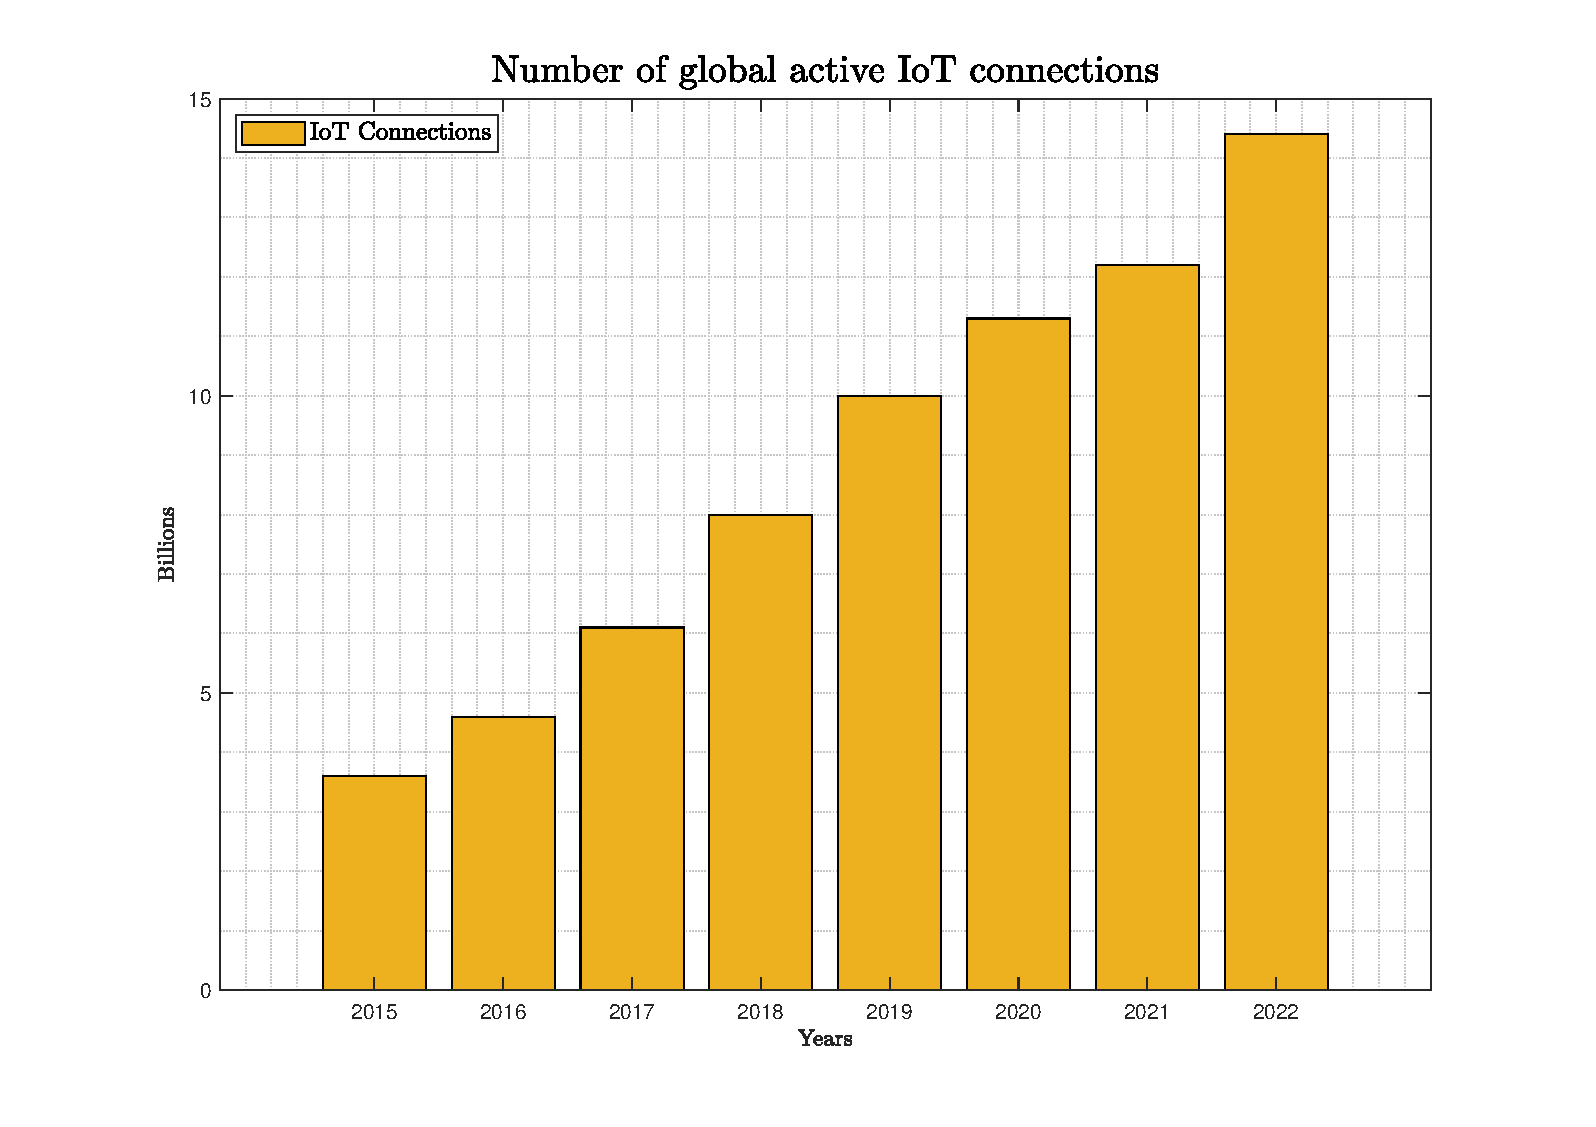
\includegraphics[width=\textwidth]{archivos/img/intro/fig_iot.eps}
    \caption{Estudio de las conexiones IoT máximas simultáneas a nivel global \cite{figuraIoTDevices}}
    \label{fig:intro_fig_iot}
\end{figure}

%6g
Por ello, se necesita una tecnología más avanzada que pueda satisfacer las futuras demandas de las redes \gls{iot}, y la arquitectura \gls{6g} se postula como una solución a todos los nuevos retos planteados. Por esa razón, para facilitar el desarrollo de las futuras redes \gls{iot} la investigación en la siguiente generación de redes moviles ha recibido mucha atención tanto por parte de academia e instituciones, como por parte de la industria \cite{Nguyen2022}. \\
\\
Si bien es cierto que la arquitectura \gls{6g} está todavía siendo formulada, se espera que esta pueda proporcionar una \gls{qos} totalmente mejorada frente a la generación anterior, dado sus prestaciones son claramente superiores, como por ejemplo, comuniaciones de latencia muy baja, tasas de velocidad de datos mejoradas y entornos inteligentes de comunicación con satelites. \\
\\
Por consiguiente, muchos de los esfuerzos de las instituciones están pasando por impulsar las redes \gls{6g}-\gls{iot} \cite{liang2021transfer}. Desde Europa se está impulsando la carrera por el \gls{6g} poniendo sobre la mesa una hoja de ruta dividida en cuatro fases diferenciadas, esperando poder finalizar en 2030 \cite{eu6GFases}. Dichos esfuerzos están siendo coordinados desde la EU’s Smart Networks and Services Joint Undertaking (SNS-JU) la cual tiene como misiones principales impulsar el despliegue del \gls{5g}, y situar a los paises miembros de la EU a la vanguardía del desarrollo de la próxima generación de redes moviles \cite{eu6gSNS}. Estas misiones planean llevarlas a cabo a través de un detallado una detallada hoja de ruta el cual se puede apreciar en la Figura \ref{fig:intro_banner_screen}.

\begin{figure}[ht]
    \centering
    \includegraphics[width=\textwidth]{archivos/img/intro/banner-screen-1.png}
    \caption{\textit{Roadmap} propuesto por el SNS-JU para el desarrollo del \glsentryshort{6g} \cite{eu6gSNS}}
    \label{fig:intro_banner_screen}
\end{figure}


Dicho \textit{roadmap} se compone de varias fases, las cuales se han subdivido en \textit{streams}. Los streams principales son cuatro, actualmente nos encontramos en el stream B del roadmap \cite{eu6GFase2}, el cual tiene como objetivo el impulso de la investigación en las areas tecnologicas habilitadoras del \gls{6g} además de la cooperación internacional con estados estrategicos como Estados Unidos. De entre todos los proyectos iniciados en 2023, destacan por ejemplo, Hexa-X~\cite{9482430}, iniciativa principal de europa liderada por Nokia financiado por el programa europeo Horizon 2020 que busca desarrollar el protipado de los sistemas \gls{6g}. Otro ejemplo, es el proyecto 6Genesis~\cite{Katz2019} financiado por Finlandia, que busca la generación de las primeras pruebas de concepto experimentales de redes \gls{6g}-\gls{iot}. Si nos vamos a proyectos más especificos, podemos encontrar ADROIT6G~\cite{ADROIT6G} y 6GTandem~\cite{6GTandem}, ambos han empezado en enero de 2023 y buscan mejorar mejorar los sistemas distribuidos de acceso al medio mediante sistemas duales en frecuencia empleando procesado de señal \gls{mimo}.\\
\\
Pero el interés en la próxima generación de redes moviles, no es meramente local. En el contexto de Estados Unidos, podemos ver cómo ya la \gls{fcc} libera espectro en la banda de los THz en US para hacer pruebas de concepto para el 6G \cite{us6g}. Algo similar sucede en Corea del Sur, donde ya han planeado lanzar un proyecto piloto de \gls{6g} para el 2026 \cite{coreaSur6G}.\\
\\
Como se puede ver, el interés por el \gls{6g} es real, y se están realizando esfuerzos exhaustivos para la proliferación de las tecnologías habilitadoras del \gls{6g}, por lo que distintas instituciones apuntan a que las primeras redes \gls{6g} que podrán ser desplegadas en 2028, pero que su comercialización y la llegada a las personas de a pie no llegará hasta el 2030 \cite{Nguyen2022}. Uno de los aspectos relevantes en la nueva generación de redes móviles, es la arquitectura de interconexión física que se va a plantear. En el \gls{5g}, ya se reaprovecho el \textit{backbone} existente de \gls{sdn}, al cual haciendo uso de flexibilidad y de la programabilidad,  se le indujeron modificaciones software para atender las nuevas especificaciones de la arquitectura planteada~\cite{Li2018}. Teniendo esto en cuenta, al lector le pueden surgir dudas de si la próxima red de \gls{6g} hará uso de las bondades de las redes \gls{sdn} para impulsar el procesamiento de datos en su arquitectura como parte del \textit{backbone}. Según los informes preliminares \cite{Uusitalo2021}~\cite{6garch1}~\cite{6garch2} que se han presentado en cuanto al diseño de la red \gls{6g}, se indica que harán uso del \gls{sdn},  junto a la tecnología \gls{p4} y técnicas de inteligencia artificial, del inglés \gls{ai}/\gls{ml}, para la definición de plano de procesamiento de datos y mejorar el rendimiento y orquestación del \textit{backbone} ya existente.\\


\section{Redes \glsentryshort{sdn}}
\label{sec:6gIoT_sdn}

%Como se ha podido ver, las redes \gls{sdn} son un hecho en las próximas redes de comuniaciones moviles \gls{6g}. Con las redes SDN, como se puede apreciar en la figura 1.1, se desea extraer el plano de control de los dispositivos intermedios de procesamiento de la red, unificándolo en entes llamados controladores, haciendo la administración de red una tarea más centralizada y flexible.

Como se ha podido ver, las redes \gls{sdn} serán una realidad en las próximas redes de comunicaciones móviles \gls{6g}. La Figura \ref{fig:sdnParadig} muestra cómo con estas redes, se pretende separar el plano de control de los dispositivos intermedios de procesamiento de la red y centralizarlo en entidades denominadas controladores, lo que permitirá una administración más flexible y centralizada de la red.\\
\\
Antes de que apareciera el concepto de \gls{sdn}, las redes convencionales solían tener un plano de control unificado en los propios dispositivos, llamado generalmente \textit{Control plane}, en el que se definía la lógica que dictaba cómo se debía llevar a cabo el forwarding de los paquetes, y un plano de datos, conocido como \textit{Data plane}, que se implementaba definiendo su datapath, compuesto por varios bloques de procesamiento para reenviar los paquetes. Sin embargo, con la aparición del paradigma de las redes \gls{sdn}, como se muestra en la Figura \ref{fig:sdnParadig}, los nodos tradicionales de la red verían cómo su plano de control sería delegado a una entidad externa llamada controlador. Este controlador tendría una perspectiva global de toda la red en su conjunto, lo que permitiría una gestión más flexible, dinámica y optimizada.

% figura sdn
\begin{figure}[ht]
    \centering
    \includegraphics[width=0.7\textwidth]{archivos/img/intro/sdn.png}
    \caption{Paradigma en las redes \glsentryshort{sdn} \cite{carrascal2020diseno}}
    \label{fig:sdnParadig}
\end{figure}

A la hora de la transmisión de la información de control desde el controlador hacia los nodos \gls{sdn}, se plantean dos puntos importantes. El primero de ellos es qué esquema en la red control se va a plantear, y la segunda que protocolo de comunicaciones se va a emplear. Empezando por los protocolos de comunicación de información de control en redes \gls{sdn}, el más utilizado es OpenFlow, aunque más adelante se verán en detalle alguno que otro más.\\
\\
En cuanto a los paradigmas de control \gls{sdn}, tenemos dos vertientes \cite{carrascal2023comprehensive}, \textbf{\textit{out-of-band}} e \textbf{\textit{in-band}}. La diferencia entre cada paradigma, ver Figura \ref{fig:sdnParadigControl}, es que en el modelo \textit{out-of-band}, cada nodo \gls{sdn} tiene un enlace dedicado con el controlador, es decir la información de control tiene una red dedicada por y para ella. El modelo \textit{in-band} por el contrario, se tiene que solo alguno/s de los nodos \gls{sdn} gestionados tiene un enlace con el controlador, y el resto de equipos emplean ese enlace para hacerle llegar al controlador la información de control. Se quiere señalar que en este último modo la información de control al no tener una red dedicada para ella misma, viajará de forma conjunta por el plano de datos hasta llegar al controlador. \\
\\
No hay un paradigma mejor que otro, cada paradigma de control tiene unos pros y unos contras, y será el caso de uso quien predisponga cuál de los dos usar. Por ejemplo, el modelo \textit{out-of-band} es un modelo mucho más caro dado que se tiene un enlace dedicado para comunicación controlador - nodo \gls{sdn}, pero por ello, también es más seguro dado que el tráfico de control está aislado. Por el contrario, el modelo \textit{in-band}, es mucho más barato dado que se emplea de red de datos para la transmisión de la información de control. Sin embargo, es un modelo más inseguro, ya que la información de control está expuesta al plano de datos.
\newpage
% fig
\begin{figure}[ht]
    \centering
    \includegraphics[width=0.8\textwidth]{archivos/img/intro/InBandOutBandScheme.pdf}
    \caption{Paradigma control en las redes \glsentryshort{sdn} \cite{carrascal2023comprehensive}}
    \label{fig:sdnParadigControl}
\end{figure}

Uno de los puntos diferenciadores entre ambos paradigmas de control, es la configuración requerida en cada caso. En el modelo de \textit{out-of-band}, no hay apenas configuración requerida, dado que, si la información es de control, tendremos una interfaz de red exclusiva con la cual trabajar. Por el contrario, en el modelo \textit{in-band}, si tenemos que tratar información de control no sabemos con qué interfaz operar. El nodo \gls{sdn} deberá saber a priori por donde reenviar los paquetes de control. Dicha configuración se obtiene de algún tipo de protocolo de comunicación \textit{in-band}, el cual proporcione a cada nodo de la red la capacidad de alcanzar el nodo que les da acceso al controlador de la red \gls{sdn}.\\
\\
Como se ha indicado anteriormente, no hay paradigma mejor que otro, cada cual ofrece unas características propias que tendrán un comportamiento mejor o peor en función del caso de uso. Por ejemplo, en un entorno \gls{iot}, donde los dispositivos a lo sumo tienen una única interfaz de comunicaciones, el modelo in-band sería ideal. El coste de añadir otra interfaz de comunicaciones no es solo monetario, sino que también impacta en la vida útil del sensor, al tener que alimentar una interfaz de comunicaciones adicional.

%En redes convencionales previas al concepto de SDN, los nodos de la red tenían unificado un plano de control, Control plane, donde se definía la lógica que dictaba como debía llevarse a cabo el forwarding de los paquetes, y un plano de datos, dataplane, el cual se puede implementar definiendo su datapath. Dicho datapath se compone de varios bloques de procesado para reenviar los paquetes. Con la llegada del paradigma de las redes SDN, como se puede apreciar en la figura 1.1, los nodos clásicos de red verían como su plano de control sería delegado a una entidad llamada controlador. El controlador tendría una perspectiva global de toda la red en su conjunto pudiendo gestionarla de una manera más flexible y centralizada.

\section{Objetivos}
\label{sec:obj}

El objetivo principal de este proyecto es conseguir el desarrollo de un protocolo de control in-band eficiente para la integración de la tecnología IoT en las futuras de redes de 6G. Como ya hemos introducido, con la llegada del IoT la dimensión de las redes va a crecer exponencialmente. Por lo consiguiente, la complejidad de la administración de dichas redes va a suponer un gran desafío. Los dispositivos IoT se podrán beneficiar de la integración con las redes SDN en 6G, ya que estas les reportará la flexibilidad y programabilidad requerida para una correcta gestión y administración de cada elemento de la red. Por ello, se pueden resumir los objetivos del proyecto en los siguientes puntos:

\begin{itemize}
    \item \textbf{Analizar el estado del arte y necesidades actuales de IoT en 6G}. Se realizará una búsqueda y recolección de información, artículos e informes sobre las demandas del \gls{iot} y las bondades preliminares del \gls{6g}.
    \item \textbf{Diseño de un protocolo in-band eficiente para IoT integrado con SDN}. Se realizará un estudio previo de las soluciones \textit{in-band} ya implementadas, se analizarán, y se propondrá una solución a medida que cubra los equipos \gls{iot} en las redes \gls{sdn}.
    \item \textbf{Emulación mediante plataformas como Contiki-NG, Mininet y ONOS}. El desarrollo inicial se probará sobre las plataformas más utilizadas en el prototipado de protocolos de comunicaciones.
    \item \textbf{Implementación y despliegue en hardware real} (tarjetas Raspberry Pi, o remotas IoT-LAB), en función de la ejecución del proyecto se estudiará la implementación del protocolo en \textit{hardware} en real.
\end{itemize}





\section{Estructura del \glsentryshort{tfm}}
\label{sec:structure}


En esta sección se indica la estructura organizativa de la memoria del proyecto \gls{tfm}, haciendo un resumen de los aspectos más significativos de cada capítulo.


\begin{description}
    \item\textbf{Capítulo 1: Introducción}. Se hará una breve introducción de la motivación principal que ha originado la realización de este \gls{tfm}, así como una breve explicación de los aspectos generales y de los objetivos que se quieren alcanzar con el trabajo presentado. Por último, se indicarán las contribuciones que se han conseguido con el mismo, en revistas científicas.

    \item\textbf{Capítulo 2: Estado del arte}. Se indicarán los conceptos fundamentales en relación al proyecto. La motivación de este capítulo es la de establecer un marco teórico lo suficientemente consistente para abordar el diseño del protocolo de comunicación \textit{in-band}.

    \item\textbf{Capítulo 3: Diseño del protocolo de control In-Band}. Se analizará soluciones anteriores \textit{in-band}, debatiendo las funcionalidades básicas que debe tener el protocolo. Se explicará el funcionamiento del mismo y se decidirá la plataforma para implementarlo.

    \item\textbf{Capítulo 4: Desarrollo y evaluación del protocolo}. Se describirá el desarrollo realizado en la plataforma elegida. Señalando aquellas partes que se consideran de mayor importancia. Por último, se incluirá una evaluación del mismo.

    \item\textbf{Capítulo 5: Conclusiones y trabajo futuro}. Se terminará la memoria de este \gls{tfm} con las conclusiones, y se presentarán las vías de trabajo a futuro que tiene este proyecto.

    \item[]\textbf{Bibliografía y referencias}. Se añadirán todos los artículos, libros, materiales consultados y empleados en la elaboración de esta memoria. Se seguirá el estilo de citación del \gls{ieee}, siguiendo las recomendaciones oficiales de la normativa sobre \gls{tfm}s de la \gls{uah}.

    \item[]\textbf{Anexos}. Se incluirán todos los manuales de usuario e instalación que se consideren oportunos. De forma adicional, se añadirán las características técnicas del \textit{hardware} con el cual se ha desarrollado este \glsentryshort{tfm}. Por último, se hará un presupuesto que incluya el coste de mano de obra, material y gastos generales.

\end{description}

\section{Contribuciones}
\label{sec:contributions}


% Papers a meter
Este \gls*{tfm} ha proporcionado significativas contribuciones a la comunidad científica, incluyendo tres publicaciones en revistas de alto impacto indexadas en el JCR (3 Q2). A continuación, se presentan estas contribuciones en resumen.\\
\\
Artículos de revistas científicas de alto impacto.

\begin{enumerate}
    \item Rojas, E., Hosseini, H., Gomez, C., \textbf{Carrascal, D.} and Cotrim, J.R., 2021. Outperforming RPL with scalable routing based on meaningful MAC addressing. Ad Hoc Networks, 114, p.102433. (JCR \textbf{Q2})
    \item Alvarez-Horcajo, J., Martinez-Yelmo, I., Rojas, E., Carral, J.A. and \textbf{Carrascal, D.}, 2022. ieHDDP: An Integrated Solution for Topology Discovery and Automatic In-Band Control Channel Establishment for Hybrid SDN Environments. Symmetry, 14(4), p.756. (JCR \textbf{Q2})
    \item \textbf{Carrascal, D.}, Rojas, E., Lopez-Pajares, D., Alvarez-Horcajo, J. and Carral, J.A., 2023. A Comprehensive Survey of In-Band Control in SDN:
          Challenges and Opportunities. Electronics, 12(6):1265. (JCR \textbf{Q2})
\end{enumerate}

%El Internet de las Cosas (del inglés \textit{Internet of Things}, \gls{iot}) \cite{iotreview} y las Redes Definidas por Software (del inglés \textit{Software-Defined Networking}, \gls{sdn}) \cite{nadeau2013sdn}, son tecnologías emergentes que desde hace unos años están revolucionando los paradigmas sobre los modelos de redes comunicaciones establecidos en el pasado. \\
%\par

%Con las redes \gls{sdn}, como se puede apreciar en la figura \ref{sdnparadigma}, se desea extraer el plano de control de los dispositivos intermedios de procesamiento de la red, unificándolo en entes llamados controladores, haciendo la administración de red una tarea más centralizada y flexible. En cuanto al \gls{iot}, se pretende interconectar billones de objetos entre sí a través de Internet con la finalidad de que exista una comunicación máquina – máquina para proveer al usuario final de entornos inteligentes. 

% \begin{figure}[h]
%     \centering
%     \includegraphics[width=6.5cm]{archivos/img/intro/sdn.png}
%     \caption{Paradigma en redes \glsentryshort{sdn}}
%     \label{sdnparadigma}
% \end{figure}

% Se considera como un punto de convergencia entre ambas tecnologías las redes 5G basadas fundamentalmente en \gls{sdn}, ya que prevén la incorporación de múltiples dispositivos \gls{iot}. Sin embargo, no todos los dispositivos \gls{iot} soportan una gestión basada en \gls{sdn} debido a las limitaciones que estos tienen en memoria, capacidad de procesamiento y  batería. Conforme el mundo de los dispositivos \gls{iot} avanza, las placas \gls{sbc} cada vez se hacen más potentes y de un tamaño más reducido, haciendo posible que éstas puedan ser incluidas como una pieza fundamental en proyectos \gls{iot} de alto rendimiento \cite{7501691}. \\

% \par

% Además, los sensores \gls{iot}, comúnmente conocidas como ``motas", continuamente se fabrican con más capacidad de procesamiento, memoria y batería con la finalidad de hacer frente a las nuevas redes de comunicaciones 5G \cite{capra2019edge}. Por todo ello,  se estima que la integración con las redes \gls{sdn} está cada vez más próxima. Generalmente, se están siguiendo estas vías de actuación:
% \begin{itemize}
%     \item \label{iot_integracionParcial}Realizar una integración parcial, haciendo uso de de dispositivos mediadores entre las motas y el core \gls{sdn}. Este dispositivo mediador, sería un dispositivo híbrido con interfaces inalámbricas y alámbricas para tener de acceso a la red \gls{sdn} \cite{7848825}.

%           \begin{figure}[h]
%               \centering
%               \includegraphics[width=10cm]{archivos/img/intro/sdn_iot.png}
%               \caption{Integración parcial de dispositivos \glsentryshort{iot} en el core \glsentryshort{sdn}}
%               \label{sdn_iot_parcial}
%           \end{figure}
%           Como se puede ver en la figura \ref{sdn_iot_parcial}, haciendo uso de un dispositivo mediador, este actuaría de pasarela o \textit{gateway} para las redes de sensores. De esta manera, se delega toda la carga de procesamiento y consumo de batería que supone integrar la interfaz de control \gls{sdn}. Además, se implementarían los distintos protocolos y estándares para comunicarse con los dispositivos \gls{iot}. Esta vía también ofrece otros aspectos positivos, entre los cuales se puede destacar, emplear el gateway como un traductor de protocolos \gls{iot} \cite{8470257}. Esto permitiría que distintos sensores que tuvieran implementados diferentes protocolos como, por ejemplo, \gls{ble}\footnote{Especificación del protocolo:  \url{https://www.bluetooth.com/specifications/}} y Zigbee\footnote{Protocolo de alto nivel basado en el estandar \gls{ieee} 802.15.4, especificación: \url{https://zigbeealliance.org/solution/zigbee/} }, pudieran interactuar entre sí a través del  gateway \gls{iot}.

%     \item \label{iot_integracionTotal}Realizar una integración total, como se puede apreciar en la figura \ref{sdn_iot_total}, donde el propio dispositivo \gls{iot} es capaz de co-existir en la red \gls{sdn}. Esta última vía es la más ambiciosa debido a que se requiere de hardware lo suficientemente potente para soportar la lógica \gls{sdn}, y de una tecnología que establezca su plano de datos de forma más eficiente posible para optimizar al máximo los recursos limitados del dispositivo.

%           \begin{figure}[ht]
%               \centering
%               \includegraphics[width=10cm]{archivos/img/intro/sdn_iot_b.png}
%               \caption{Integración total de dispositivos \glsentryshort{iot} en el core \glsentryshort{sdn}}
%               \label{sdn_iot_total}
%           \end{figure}

% \end{itemize}



% \section{Tecnologías para la definición del datapath}



% En redes convencionales previas al concepto de \gls{sdn}, los nodos de la red tenían unificado un plano de control, \textit{Control plane}, donde se definía la lógica que dictaba como debía llevarse a cabo el \textit{forwarding} de los paquetes, y un plano de datos, \textit{Data plane}, el cual se puede implementar definiendo su datapath. Dicho datapath se compone de varios bloques de procesado para reenviar los paquetes. Con la llegada del paradigma de las redes \gls{sdn}, como se puede apreciar en la figura \ref{sdnparadigma}, los nodos clásicos de red verían como su plano de control sería delegado a una entidad llamada controlador. El controlador tendría una perspectiva global de toda la red en su conjunto pudiendo gestionarla de una manera más flexible y centralizada. \\
% \par
% En consecuencia, los nodos de la red estarían destinados a implementar un plano de datos, y una interfaz de control para ser configurados por el controlador mediante protocolos como, por ejemplo, OpenFlow\footnote{\url{https://www.opennetworking.org/software-defined-standards/specifications/}}. \\
% \par
% Por lo tanto, para ejecutar la integración de los dispositivos \gls{iot} en las redes \gls{sdn} se debe poder definir un datapath en dichos dispositivos y que estos posean una interfaz de control para ser configurados desde un hipotético controlador. Debido a esto, se requiere hacer uso de tecnologías que nos permitan definir el plano de datos de estos dispositivos. En este \gls{tfg}, se abordarán las siguientes tecnologías:

% \begin{itemize}
%     \item El lenguaje \textbf{P4}. Este lenguaje de alto nivel nos permite definir el procesado de los paquetes para un conjunto de arquitecturas. Dichas arquitecturas tienen su propia especificación. Con ello, se quiere conseguir que los programas P4 sean independientes del \textit{hardware} donde se ejecute \cite{2014p4}.

%     \item \textbf{\gls{xdp}}. Es un \textit{framework} programable y de alto rendimiento para el procesado de paquetes en el Kernel de Linux. El procesado de los paquetes se lleva a cabo en el punto más bajo de la pila de red de Linux, consiguiendo así añadir nuevas funcionalidades sin necesidad de modificar el propio Kernel. Además, el hecho de definir el procesado de paquetes casi en la propia interfaz, reporta un gran rendimiento ya que no es necesario atravesar toda la pila de protocolos, con todo lo que eso conlleva (reservas de memoria, reservas de memoria para metadatos, encolado de los paquetes, desencapsulado de cabeceras, análisis y tratamiento de cabeceras, etc) \cite{xdp1}.
% \end{itemize}



% \section{Objetivos}

% El objetivo de este proyecto es realizar un estudio y análisis de las tecnologías P4 y \gls{xdp} para la integración de dispositivos \gls{iot} en entornos \gls{sdn}. Como ya hemos introducido, con la llegada del \gls{iot}, la dimensión de las redes va a crecer exponencialmente. Por consiguiente, la complejidad de la administración de dichas redes va a suponer un gran desafío.  Los dispositivos \gls{iot} se podrán beneficiar de la integración con las redes \gls{sdn}, ya que éstas les reportarán la \textbf{flexibilidad} y \textbf{programabilidad} requerida para una correcta gestión y administración de cada elemento de la red. Para alcanzar dicho objetivo, se han planteado los siguientes puntos:

% \begin{itemize}
%     \item \textbf{Documentación y estudio}: Búsqueda y recolección de información, artículos y guías para tener
%           los conocimientos básicos necesarios sobre el estado del arte actual y de las tecnologías para definir el plano de datos. De esta forma, se podrá plantear los diseños y desarrollos más optimizados, de cara a favorecer las limitaciones impuestas por los dispositivos \gls{iot}.

%     \item \textbf{Planteamiento de casos de uso típicos y elección de escenarios}: Se hará un planteamiento de funcionalidades básicas, casos de uso, que una tecnología que define un datapath debe ser capaz de proveer. Además, se elegirán los escenarios y plataformas para desplegar dichos casos de uso.

%     \item  \textbf{Desarrollo de los casos de uso}: Se abordará el desarrollo de dichos casos de uso con ambas tecnologías (P4, \gls{xdp}) en los escenarios planteados. Se tratará que los escenarios donde se desplieguen los desarrollos sean lo más homogéneos posibles, para que los puntos fuertes y débiles de cada tecnología puedan ser esclarecidos.

%     \item \textbf{Evaluación y comprobación de funcionamiento}: Se comprobará el correcto funcionamiento de todos los casos de uso desarrollados y por último, se evaluará que tecnología es más idónea para definir el datapath de los dispositivos \gls{iot} en su integración en entornos \gls{sdn}.
% \end{itemize}


% \section{Estructura del \glsentryshort{tfg}}

% En esta sección se indica la estructura básica de este \gls{tfg}, haciendo un breve resumen de los aspectos más importantes y significativos de cada capítulo.


% \begin{description}
%     \item\textbf{Capítulo 1: Introducción}. Se hará una breve introducción de la motivación que ha originado la realización de este \gls{tfg}, así como una breve explicación de los aspectos generales y de los objetivos que se quieren alcanzar con el trabajo presentado.

%     \item\textbf{Capítulo 2: Estado del arte}. Se documentarán conceptos fundamentales en relación al proyecto, además de todas las diferentes herramientas que sean utilizadas. La motivación de este capítulo es la de establecer un marco teórico lo suficientemente consistente para abordar el análisis y el diseño de forma óptima, previo al desarrollo.

%     \item\textbf{Capítulo 3: Diseño y análisis de casos de uso}. Se debatirá y analizará que funcionalidades básicas deben tener las distintas tecnologías para definir el datapath. Para ello, se diseñarán distintos casos de uso para así demostrar la eficiencia de una tecnología sobre la otra en la integración de los dispositivos \gls{iot} en entornos \gls{sdn}.

%     \item\textbf{Capítulo 4: Desarrollo y evaluación de casos de uso}. Se describirá el desarrollo realizado, indicando las partes más importantes de cada caso de uso, ofreciendo al final de cada caso una evaluación de su funcionamiento.

%     \item\textbf{Capítulo 5: Conclusiones y trabajo futuro}. Se terminará la memoria con las conclusiones del trabajo realizado, y se presentarán las vías de trabajo futuro que tiene este proyecto.

%     \item[]\textbf{Bibliografía y referencias}. Se añadirán todos los artículos, libros, materiales consultados y empleados en la elaboración de esta memoria. Se seguirá el estilo de citación del \gls{ieee}, siguiendo las recomendaciones oficiales de la normativa sobre \gls{tfg}s de la \gls{uah}.

%     \item[]\textbf{Anexos}. Se incluirán todos los manuales de usuario e instalación que se consideren oportunos. De forma adicional, se añadirán las características técnicas del \textit{hardware} con el cual se ha desarrollado este \glsentryshort{tfg}. Por último, se hará un presupuesto que incluya el coste de mano de obra, material y gastos generales.

% \end{description}

%%%%%%%%%%%%%%%%%%%%%%%%%%%%%%%%%%%%%%%%%%%%%%%%%%%%%%%%%%%%%%%%%%%%%%%%%%%%%%%%%%%%%%%%%%%%%%%%%%%%
%\chapter{Estado del arte}
\label{estadoArte}

En este capítulo se documentarán los conceptos fundamentales en relación al proyecto, además de todas las diferentes herramientas que sean utilizadas mayoritariamente. La motivación de este capítulo es la de establecer un marco teórico lo suficientemente consistente para abordar el análisis y el diseño de forma óptima, previo al desarrollo. Por último, se mencionará las contribuciones y la documentación generada con la intención de divulgar los contenidos de este proyecto a través de la herramienta \textit{GitHub}.


%%%%%%%%%%%%%%%%%%%%%%%%%%%%%%%%%%%%%%%%%%%%%%%%%%%%%%%%%%%%%%%%%%%%%%%%%%%%%%%%%%%%%%%%%%%%%%%%%%%%%
% 6G
%%%%%%%%%%%%%%%%%%%%%%%%%%%%%%%%%%%%%%%%%%%%%%%%%%%%%%%%%%%%%%%%%%
\section{Red de comunicación \glsentryshort{6g}}
\label{sec:6g}

Las redes de comunicación de sexta generación, están en desarrollo para ofrecer una conectividad aún más rápida, confiable y eficiente que las generaciones anteriores. A medida que la demanda de datos continúa creciendo exponencialmente y surgen nuevas aplicaciones y tecnologías, como el \gls{iot}, la realidad aumentada y la \gls{ai}, se espera que el \gls{6g} proporcione una infraestructura de red sólida y escalable para satisfacer estas necesidades futuras. Los principales puntos claves de esta nueva generación se pueden resumir en los siguientes puntos.

\begin{itemize}

\item Velocidad y capacidad extremadamente altas: Una de las principales características del \gls{6g} será la velocidad y capacidad extremadamente altas, superando con creces las capacidades del \gls{5g}. Se espera que el \gls{6g} alcance velocidades de terabits por segundo, lo que permitirá una transmisión de datos ultra rápida y un soporte eficiente para aplicaciones de alta demanda, como son la transmisión de video en 8K, realidad virtual y realidad aumentada de alta calidad.

\item Latencia ultrabaja: El \gls{6g} aspira a lograr una latencia ultrabaja, reduciendo aún más el tiempo de respuesta de la red. Se espera que la latencia en el \gls{6g} sea de solo unos pocos milisegundos, lo que permitirá aplicaciones en tiempo real de misión crítica, como cirugías remotas, vehículos autónomos y aplicaciones de realidad virtual y aumentada altamente interactivas.

\item Conectividad ubicua: El \gls{6g} tiene como objetivo proporcionar conectividad ubicua, extendiéndose más allá de las áreas urbanas y llegando a áreas remotas y rurales haciendo uso de radio enlaces satelitales de orbita baja (LEO). Se espera que el \gls{6g} aborde la brecha digital y brinde conectividad global a nivel mundial, permitiendo una mayor inclusión digital y oportunidades equitativas para todos.

\item Integración de tecnologías emergentes: El \gls{6g} se construirá sobre tecnologías emergentes, como inteligencia artificial (IA), \gls{ml}, llegando a proponer la computación cuántica y nanotecnología. Estas tecnologías avanzadas permitirán el desarrollo de sistemas de red más inteligentes y autónomos, optimizando la eficiencia y la capacidad de adaptación de la red.

\item Sostenibilidad y eficiencia energética: El \gls{6g} se enfocará en la sostenibilidad y la eficiencia energética para reducir su impacto ambiental. Se espera que las redes \gls{6g} sean más eficientes en términos de consumo de energía, al tiempo que brinden una mayor capacidad y rendimiento. Además, se explorarán nuevas técnicas de transmisión de energía y comunicación inalámbrica para impulsar la eficiencia energética en dispositivos y redes.

\end{itemize}

\subsection{Tecnologías habilitadoras}

Como se comentó en el capítulo de introducción (Capitulo \ref{ch:intro}), esta nueva generación aún es prematura y no tiene unos estándares claros y definidos sobre como se va a llevar a cabo, sin embargo, ya empieza a haber propuestas sobre las tecnologías habilitadoras que harán del \gls{6g} una realidad tarde o temprano. Desde el proyecto líder europeo  6G-Flagship y la organiazción One6G ya se apuntan a una serie de tecnologías claves, las cuales, se indican a continuación.

\subsubsection{Banda de los THz}

Según se ha indicado, con el \gls{6g}, se espera que fusione los mundos digital y físico en todas sus dimensiones, brindando a los usuarios una experiencia holográfica, háptica y multisensorial. Según la \gls{itu}, estas aplicaciones surgirán en la próxima década y se caracterizarán por requerir comunicaciones altamente exigentes \cite{fg20192030}. Además, algunas aplicaciones demandarán funcionalidades que los sistemas móviles actuales no proporcionan, como una detección precisa, mapeo y localización. Un ejemplo destacado de caso de uso es la telepresencia holográfica\footnote{\url{https://blogthinkbig.com/peoplefirst/telepresencia-holografica}}. La transmisión de hologramas 3D en su forma más básica requiere una capacidad de más de 4 Tbps \cite{giordani2020toward}. La capacidad de detectar y comprender el entorno permitirá a la red predecir el movimiento de los usuarios sin información explícita, creando así una experiencia inmersiva a distancia. Asimismo, las comunicaciones de alta velocidad de datos y baja latencia necesarias para la automatización de fábricas se beneficiarán de las transmisiones a terabits por segundo (Tbps). \\
\\
Con el fin de satisfacer esta necesidad, las comunicaciones en terahercios (THz) se han identificado como una opción prometedora para la capa física en 6G, ya que tienen el potencial de permitir velocidades de datos de terabits por segundo y ofrecer servicios de detección, mapeo y localización \cite{latva2020key}. En la Conferencia Mundial de Radiocomunicaciones de 2019 (CMR2019)\footnote{\url{https://www.itu.int/es/ITU-R/conferences/wrc/2019}}, la \gls{itu} identificó un espectro de 137 GHz entre 275 y 450 GHz que se puede utilizar para las comunicaciones en terahercios \cite{kurner2020impact}. Esto se suma al espectro ya asignado por debajo de los 275 GHz, lo que proporciona un total de 160 GHz en la gama de sub-terahercios. En 2017, el grupo de trabajo IEEE 802 completó el primer estándar inalámbrico para frecuencias portadoras alrededor de los 300 GHz (IEEE Std 802.15.3d-2017) \cite{ieee2017ieee, petrov2020ieee}. Esto establece una base sólida para el desarrollo y la implementación de las comunicaciones en terahercios en el contexto de 6G. Aunque, también aparecen nuevos retos de capa física a solventar, dado que según subimos en frecuencia la atenuación de la señal aumentará de forma cuasi-proporcional.

\subsubsection{Próxima generación de \glsentryshort{mimo}}

Utilizar múltiples antenas conlleva una serie de ventajas fundamentales. Estas ventajas están condicionadas por el conocimiento del canal en el transmisor y/o receptor, las propiedades del canal de propagación (como características multitrayecto y atenuación) y el tipo de enlace, ya sea punto a punto o multiusuario. Además, la cooperación entre las señales transmitidas o recibidas y el procesamiento conjunto de las antenas también juegan un papel importante.\\
\\
El diseño de soluciones de múltiples entradas y múltiples salidas (\gls{mimo}, por sus siglas en inglés) depende en gran medida del escenario específico que se considere, pero generalmente se suele plantear una descomposición generica del canal donde se vaya a trabajar en una serie de subcanales $M$ paralelos (Ver figura \ref{fig:fig_3}). No existe una única solución \gls{mimo} universal. Al diseñar sistemas \gls{mimo}, es esencial tener en cuenta las limitaciones prácticas y encontrar un equilibrio entre las ganancias básicas del \gls{mimo} \cite{ordonez2011fundamental}. Las ganancias de estos sistemas se pueden resumir en los siguientes puntos.

\begin{itemize}
    \item Ganancia por procesado en \textit{Array}. La combinación coherente de $M$ antenas, sin importar la distancia entre ellas o si funcionan en modo de transmisión o recepción, puede mejorar la relación señal-ruido (SNR) en un máximo de 10 veces. En otras palabras, la SNR puede mejorarse en un máximo de $10*log_{10}(M)\:dB$ mediante la técnica de combinación de las $M$ antenas. Esto se logra mediante la formación de haz (\textit{beamforming}), la cual nos permite ``apuntar" de una forma más precisa con el lóbulo principal de nuestro diagrama de radiación al sistema receptor. Existen múltiples técnicas para llevar a cabo un \textit{beamforming}, desde alimentaciones diferentes en las $M$ antenas, a desfases, jugando con la combinación resultante de todas ellas.

    \item Multiplexación y ganancia por acceso múltiple. La combinación de antenas proporciona otra ventaja fundamental, la capacidad de eliminar señales no deseadas controlando los pesos de las antenas de tal manera que los frentes de onda superpuestos se cancelen en canales específicos. Esto se aprovecha de varias formas, como en el caso del acceso múltiple por división espacial (SDMA) en canales multiusuario o en la multiplexación espacial en canales punto a punto. En general, se asume que el número de señales es igual o menor al número de antenas. Con un conjunto de $M$ antenas, es posible separar hasta $M$ usuarios sin interferencias. Esta capacidad de separación espacial permite mejorar significativamente la eficiencia y el rendimiento de los sistemas de comunicación, al permitir la transmisión simultánea y la recepción de múltiples señales independientes en el mismo espectro.

    \item   La diversidad de antenas y \textit{hardening} del canal. Son conceptos relacionados con los desvanecimientos causados por la propagación multitrayecto. A pequeña escala, estos desvanecimientos espaciales pueden ocurrir debido a la presencia de múltiples trayectos de señal. Si las distancias entre las antenas son lo suficientemente grandes, cada antena experimentará un canal que no está correlacionado con las demás antenas. Este fenómeno se aprovecha transmitiendo o recibiendo información redundante en paralelo a través de las múltiples antenas. Al hacerlo, se logra una diversidad espacial en el sistema, lo que implica que cada antena experimenta diferentes condiciones de desvanecimiento. Como resultado, si una antena se ve afectada por un desvanecimiento, es probable que otras antenas no se vean afectadas de la misma manera. Esta diversidad de antenas proporciona robustez al canal frente a los desvanecimientos. Al transmitir o recibir información redundante a través de múltiples antenas, se pueden mitigar los efectos de los desvanecimientos selectivos de trayecto y mejorar la calidad de la señal. 
\end{itemize}    

\begin{figure}[h!]
    \centering
    \includegraphics[width=0.8\textwidth]{archivos/img/teoria/fig_3.pdf}
    \caption{Descomposición genérica de un canal \gls{mimo} en subcanales paralelos}
    \label{fig:fig_3}
\end{figure}

Con el fin de aprovechar al máximo las ganancias del \gls{mimo}, se ha observado una tendencia hacia arrays de antenas cada vez más grandes, ya sea en configuraciones coubicadas, conocido como ``massive MIMO" \cite{bjornson2016massive}, o distribuidos en toda la zona de servicio. En respuesta a esta tendencia, se introdujo el \gls{mimo} de dimensión completa en la versión 13 del estándar LTE. En el caso de 5G NR, el 3GPP especificó 32 antenas en la versión 15, y se espera que este número aumente en futuras versiones para habilitar el \gls{mimo} masivo. En el ámbito de la \gls{6g}, se ha introducido el concepto de múltiples matrices D-MIMO, conocido como \gls{mimo} masivo modular (mmMIMO) \cite{jeon2021mimo}. Este concepto incluye D-MIMO estructurado y diversas variantes de CoMP (Coordinated Multi-Point), incluyendo la transmisión conjunta como casos especiales. En \cite{jeon2021mimo} se presentan ejemplos de implementación de prototipos y se describen los pasos de normalización asociados.\\
\\
Estas tendencias en la evolución del \gls{mimo} reflejan la importancia de utilizar arrays de antenas cada vez más grandes y distribuidos para mejorar el rendimiento y la capacidad de los sistemas de comunicación. El enfoque en el \gls{mimo} masivo y el mmMIMO en el \gls{6g} tiene como objetivo proporcionar una mayor capacidad y eficiencia espectral, así como mejorar la cobertura y la calidad de la señal en entornos complejos. 

\subsubsection{\glsentryshort{ai} federada y distribuida}
 
\subsubsection{Plano de datos inteligente}

\subsubsection{Infraestructuras flexibles y programables }
   



\subsection{Casos de uso verticales}



En resumen, el \gls{6g} promete llevar la conectividad y las comunicaciones inalámbricas a un nuevo nivel, superando las capacidades del \gls{5g} y habilitando una amplia gama de aplicaciones y servicios avanzados. Con velocidades ultra altas, latencia ultrabaja, conectividad ubicua y la integración de tecnologías emergentes, el \gls{6g} está destinado a impulsar la transformación digital en diversas industrias y habilitar un futuro aún más conectado e inteligente.



%%%%%%%%%%%%%%%%%%%%%%%%%%%%%%%%%%%%%%%%%%%%%%%%%%%%%%%%%%%%%%%%%%%%%%%%%%%%%%%%%%%%%%%%%%%%%%%%%%%%%
% IoT
\section{Tecnología \glsentryshort{iot}}
\label{iot}

La premisa básica de la tecnología \gls{iot} \cite{iotreview} conectar cualquier dispositivo que tenga cierta capacidad de cómputo. Esto significa que los objetos que actualmente no están conectados a Internet, estarán conectados de manera que puedan comunicarse e interactuar con personas y otros objetos. \\
\par

La tecnología \gls{iot} es una transición tecnológica en la que los dispositivos al ser dotados de inteligencia por estar conectados a Internet podrán proveer de entornos inteligentes a los humanos.  Cuando los objetos puedan ser controlados a distancia a través de una red, se habilitará una integración más estrecha entre el mundo físico y las máquinas, permitiendo mejoras en las áreas de medicina, automatización y logística \cite{7073822}.\\
\par

El ecosistema \gls{iot} es amplio, e incluso se puede parecer un poco caótico debido a la gran cantidad de componentes y protocolos que abarca. Es recomendable en vez de ver el \gls{iot} como un termino único, verlo como un paraguas de varios conceptos, protocolos y tecnologías, enfocados a un mismo propósito de interconectar ``Cosas" a Internet. Si bien la amplia mayoría de elementos \gls{iot} están diseñados para aportar numerosos beneficios en las áreas de productividad y automatización, al mismo tiempo introducen nuevos desafíos, como por ejemplo la gestión de la gran cantidad de dispositivos que van a aparecer en las redes, y la cantidad de datos y mensajes que todos estos generaran \cite{iotreview}.

\subsection{Arquitectura}

Aunque en el ecosistema hay diferentes \textit{stacks} de protocolos, todos ellos se pueden resumir en la siguiente arquitectura básica \cite{iotreview}.

\begin{itemize}
    \item \textit{Perception Layer}, en esta capa se da un significado físico a cada objeto. Consiste en sensores de diferentes tipos como etiquetas RFID, sensores IR u otras redes de sensores que podrían detectar la temperatura, la humedad, la velocidad y la ubicación, etc. Esta capa recolecta información útil a partir de los sensores vinculados a los objetos,  convierte dicha información en señales digitales que más tarde se delegarán a la Capa de Red para su posterior transmisión.
    
    \item \textit{Network Layer}, el propósito de esta capa es la de recibir la información en
    forma de señales digitales desde la capa de Percepción y transmitirla a los sistemas de procesamiento en la capa de \textit{Middleware}. Esto se llevará a cabo a través de las distintas tecnologías de acceso como WiFi, BLE, WiMaX, ieee802154 y con protocolos como IPv4, IPv6, MQTT.
    
    \item \textit{Middlware Layer}, en esta capa se procesa la información recibida de todos los sensores. En esta capa se puede incluir las tecnologías como Cloud computing, o sistemas gestores,  que aseguran un acceso directo a bases de datos donde se puede almacenar toda la información recolectada. Teniendo una gran cantidad de información centralizada, generalmente se aplican sistemas de inteligencia artificial para procesar la información, y tomar decisiones predictivas totalmente automatizadas. Estos sistemas suelen ser utilizados para analizar el tiempo, contaminación o tráfico en las ciudades. 
    
    \item \textit{Application Layer}, la finalidad de  esta  capa es la de realizar las aplicaciones \gls{iot} para el usuario final. Estas aplicaciones se valdrán de los datos procesados para ofrecer funcionalidades al usuario final, por ejemplo, una aplicación del tiempo.
    
    \item \textit{Business Layer}, esta capa aunque es un poco abstracta, se suele añadir para representar la gestión de múltiples las aplicaciones y servicios \gls{iot}. 
\end{itemize}

% Foto 
\begin{figure}[ht]
    \centering
    \includegraphics[width=6.5cm]{archivos/img/teoria/arch_edited.png}
    \caption{Arquitectura básica \glsentryshort{iot}}
    \label{fig:iotBasicArch}
\end{figure}

\subsection{Topologías}

Entre las tecnologías de acceso disponibles para conectar los dispositivos de \gls{iot}, dominan tres esquemas topológicos principales, estrella, malla y p2p. Para las tecnologías de acceso de largo y corto alcance, predomina la topología de estrella, como se puede encontrar en las redes datos móviles, LoRa y BLE. Las topologías en estrella utilizan una única estación base central para permitir las comunicaciones con los nodos finales. En cuanto a las tecnologías de mediano alcance, se pueden encontrar topologías en estrella, de p2p o en malla, como se ve en la figura \ref{fig:iotTopo}. Generalmente se suele hacer uso de un tipo de topología sobre otra en función de las limitaciones de los nodos que la conforman \cite{iotbook}.\\
\par

% Foto 
\begin{figure}[ht]
    \centering
    \includegraphics[width=7.5cm]{archivos/img/teoria/iot_topo.jpg}
    \caption{Tipos de topología con dispositivos \glsentryshort{iot} \cite{iotbook}}
    \label{fig:iotTopo}
\end{figure}


\subsection{Redes LLN}

Las redes de baja capacidad, conocidas como, \gls{lln}\footnote{\url{https://tools.ietf.org/html/rfc7228}}, se caracterizan por estar compuestas de dispositivos (sensores, motas) con limitaciones de memoria, batería y procesamiento. Dichos nodos, se interconectarán haciendo uso de distintos de tipos de enlace, como por ejemplo \texttt{ieee802154} ó LowPower-WiFi \cite{llnrfc}. Este tipo de redes pueden estar presentes en distintos campos de aplicación, entre las que se incluyen asistencia sanitaria, monitorización industrial, redes de sensores, etc.   \\

\par
Otra condición de las redes \gls{lln}, son las pérdidas en capa física debidas a las interferencias y variabilidad de los ``complicados" entornos radio donde estarán desplegadas dichas redes. Por ello, y teniendo en cuenta que los nodos que formarán parte de las redes \gls{lln} serán de baja capacidad, es necesario que los protocolos utilizados en esta red sean capaces de optimizar al máximo los recursos de los dispositivos \cite{iotbook}. 

\subsubsection{IEEE 802.15.4}

El estándar \texttt{ieee802154}\footnote{\url{https://tools.ietf.org/id/draft-ietf-lwig-terminology-05.html}} define la tecnología acceso a un entorno inalámbrico (\textit{phy} y \textit{mac}) para dispositivos de baja capacidad (limitados en batería y capacidad de transmisión). Este estándar se caracteriza por la optimización de los recursos del nodo en cuestión, consiguiendo una duración prolongada de la batería, además, esta tecnología de acceso permite un fácil uso utilizando un \textit{stack} de protocolos compacto, al tiempo que sigue siendo simple y flexible. Por todas estas características, el estándar \texttt{ieee802154} es usado en la mayoría de \textit{stack} de protocolos enfocados al \gls{iot}. Uno de los más utilizados es el \textit{stack} 6LoWPAN, definido por el \gls{ietf}, consiste en una capa de adaptación de IPv6 sobre las capas del estándar \texttt{ieee802154} (Ver figura \ref{fig:6lowapan}) \cite{6lowpan}.\\
\par

\vspace{0.5cm}

% Foto 
\begin{figure}[ht]
    \centering
    \includegraphics[width=12cm]{archivos/img/teoria/6LoWPAN-Protocol-Stack.png}
    \caption{Pila de protocolos 6LoWPAN \cite{6lowpan}}
    \label{fig:6lowapan}
\end{figure}



%%%%%%%%%%%%%%%%%%%%%%%%%%%%%%%%%%%%%%%%%%%%%%%%%%%%%%%%%%%%%%%%%%%%%%%%%%%%%%%%%%%%%%%%%%%%%%%%%%%%%
% SDN
\section{Redes  \glsentryshort{sdn}}
\label{sec:sdn}


El paradigma \gls{sdn} \cite{nadeau2013sdn} se refiere a una arquitectura de red en la que se separa el plano de control de la red para centralizarlo en un controlador único. Esta estructura permite lograr una administración de red más centralizada y flexible \cite{nadeau2013sdn}. La idea del \gls{sdn} comenzó a gestarse en la Universidad de Stanford en 2003, cuando el profesor asociado de ese entonces, Nick McKeown, planteó las limitaciones de las redes convencionales y la necesidad de replantear cómo operaban los \textit{backbones} \cite{sdnBegins}. En 2011, se acuñó el término \gls{sdn}, al mismo tiempo que se lanzó la organización \gls{onf} \cite{onf}, encargada de establecer estándares y promover la difusión del \gls{sdn}.

\subsection{Arquitectura del paradigma \glsentryshort{sdn}}

La arquitectura \gls{sdn} se destaca por su dinamismo, rentabilidad y adaptabilidad, lo que la convierte en una solución ideal para las demandas actuales de las redes de comunicaciones. Como se ha mencionado anteriormente, esta arquitectura se basa en la separación del plano de control y el plano de datos, trasladando el control a una entidad central llamada controlador. A través de esta entidad, se ofrecen interfaces que permiten a las aplicaciones de servicios de red utilizarlas. Esto hace que el control de la red sea programable directamente, lo que agiliza y dinamiza su gestión.\\
\\
La arquitectura \gls{sdn} se divide en tres capas, como se muestra en la Figura \ref{fig:sdnBasicArch}. La primera capa es el plano de datos, donde se encuentran todos los elementos de red responsables del reenvío de los datos. La segunda capa es el plano de control, compuesto por diferentes controladores \gls{sdn}. Por último, la capa de aplicación alberga todas las aplicaciones que se comunican con el controlador \gls{sdn}.\\
\\
Estas capas se comunican entre sí a través de interfaces abiertas. Por ejemplo, la interfaz \textit{Southbound} permite programar el estado de reenvío de los elementos de red en el plano de datos. Por otro lado, la interfaz \textit{Northbound} permite la comunicación entre las aplicaciones y los controladores \gls{sdn}, permitiendo la obtención de datos y el ajuste de parámetros mediante una API-Rest. Además, existen otras interfaces, como \textit{Westbound} y \textit{Eastbound}, que se han consolidado en los últimos años para interconectar controladores y establecer políticas comunes entre diferentes dominios \gls{sdn}.\\

% Foto 
\begin{figure}[ht]
    \centering
    \includegraphics[width=0.9\textwidth]{archivos/img/teoria/sdn_arch.png}
    \caption{Arquitectura típica \glsentryshort{sdn} \cite{carrascal2020diseno}}
    \label{fig:sdnBasicArch}
\end{figure}


\subsection{Protocolo OpenFlow}

Existen varios protocolos para el control de los elementos de red desde el controlador, pero el más ampliamente utilizado es OpenFlow. OpenFlow es un protocolo de la interfaz \textit{Southbound} que establece la comunicación entre los controladores \gls{sdn} y los elementos de red para configurar el plano de forwarding de estos últimos. La especificación de este protocolo está definida por la \gls{onf}\footnote{\url{https://www.opennetworking.org/software-defined-standards/specifications/}}, y cuenta con varias versiones, siendo la más reciente la versión \texttt{1.5.1} lanzada en 2015.\\
\\
El concepto fundamental en OpenFlow es el flujo (\textit{flow}), el cual está compuesto por paquetes que se han clasificado según reglas específicas. Estas reglas se encuentran en las tablas de flujo (\textit{flow table}) y suelen estar relacionadas con los puertos de entrada o los valores de los campos de cabecera del paquete. Cuando los criterios de una regla coinciden con los valores de un paquete entrante, se produce una coincidencia (\textbf{\textit{match}}).\\
\\
Cuando se produce una coincidencia (\textit{match}), el paquete se somete a una serie de instrucciones asociadas a la regla con la que ha coincidido. Estas instrucciones pueden incluir la medición del paquete, la aplicación de acciones específicas o el enrutamiento hacia otra tabla de flujo. De esta manera, al completar las tablas de flujo con reglas suministradas por el controlador \gls{sdn}, se configura el estado de reenvío del switch en cuestión \cite{nadeau2013sdn}. A continuación, en la Figura \ref{fig:openflow_arch}, se puede apreciar los elementos básicos que suele contener un switch Openflow. Más adelante en la Sección \ref{subsec:BOFUSS} sobre \textit{software switches} se estudiarán en profundidad los elementos básicos que componen un agente \gls{sdn} que implementa un agente Openflow.


\begin{figure}[ht]
    \centering
    \includegraphics[width=0.6\textwidth]{archivos/img/teoria/openflow_arch.png}
    \caption{Arquitectura básica de agente OpenFlow \cite{fernandes2015software}}
    \label{fig:openflow_arch}
\end{figure}


%%%%%%%%%%%%%%%%%%%%%%%%%%%%%%%%%%%%%%%%%%%%%%%%%%%%%%%%%%%%%%%%%%%%%%%%%%%%%%%%%%%%%%%%%%%%%%%%%%%%%
% Linux Networking
\section{Linux Networking}
\label{sec:linuxNetworking}

Esta sección recopilará todos los conceptos y herramientas relacionadas con la parte de Networking en Linux, que son fundamentales para el desarrollo, análisis y validación de este proyecto.


%%%%%%%%%%%%%%%%%%%%%%%%%%%%%%%%%%%%%%%%%%%%%%%%%%%%%%%%%%%%%%%%%%%%%%%%%%%%%%%%%%%%%%%%%%

\subsection{Interfaz virtual - \texttt{tun/tap}}
\label{linuxNetworking_tuntap}

En el mundo de las redes siempre se habla de las interfaces tun/tap de forma indistinta cuando van a utilizarse, sin embargo, cada una tiene su cometido. Como se ha indicado, en networking, las interfaces TUN/TAP son interfaces virtuales que se crean y se gestionan en espacio de kernel. Mencionar que como estas interfaces son virtuales y se gestionan directamente vía softaware, no como las interfaces reales que se gestionan con unos drivers diferentes, cada interfaz con su driver específico de la interfaz.  Los drivers de las interfaces TUN/TAP se crearon en los 2000 como una unión de los avances de los drivers desarrollados en las comunidades de Solaris, Linux, BSD. Actualmente los drivers solo tienen mantenimiento por los kernels de linux y FreeBSD. Ambos tipos de interfaces se utilizan para tunelado, pero no pueden ser utilizadas a la vez dado que trabajan en niveles distintos. Las TUN, de \textit{network \textbf{TUN}nel}, emula la capa de red y puede llegar hacer reenvío de los paquetes. En cambio las interfaces TAP,  trabajan en capa 2 solo en capa dos, y emulan un equipo que trabaja en dicha capa, como por ejemplo un switch \cite{tuntap1}. Por tanto, hay que dejar claro lo que se puede llegar a realizar con cada interfaz (Ver figura \ref{fig:linux1}).

\begin{itemize}
    \item \texttt{TUN} se puede llegar a utilizar para routing.
    \item \texttt{TAP} se puede llegara utilizar para crear un bridge.
\end{itemize}

Generalmente, cuando los paquetes son enviados por el sistema operativo a través de una interfaz TUN/TAP,  serán recibidos por algún programa de espacio de usuario, el cual, está enganchado directamente en la interfaz. Cualquier programa de espacio de usuario podrá pasar paquetes por las interfaces, y las interfaces virtuales se lo pasarán al \textit{stack} de red por defecto, emulando la recepción de los paquetes inyectados desde espacio de usuario.

% fig
\begin{figure}[ht]
    \centering
    \includegraphics[width=\textwidth]{archivos/img/teoria/linux1.png}
    \caption{Diagrama de funcionamiento de las interfaces virtuales TUN/TAP \cite{tuntap2}}
    \label{fig:linux1}
\end{figure}

Para la creación de estas interfaces lo podemos hacer por ioctl o podemos hacerlo más fácil a través del binario tunctl o en su defecto con el comando de \texttt{tuntap} del set de herramientas iproute2. A continuación, en el bloque \ref{code:tun_tap_use} se indican todos los comandos necesarios para trabajar con las interfaces TUN/TAP.

\begin{lstlisting}[language= bash, style=Consola, caption={Manejo de interfaces TUN - TAP},label=code:tun_tap_use]
    # En caso de querer utilizar tunctl hay que instalar el binario
    sudo apt install -y uml-utilities
    
    # Para crear una un interfaz podemos hacer lo siguiente
    tunctl -t {nombre_tun}

    # Para eliminarla
    tunctl -d {nombre_tun}

    # Para crear interfaces de tipo TAP hay que hacer lo siguiente
    tunctl -p -t {nombre_tun}
    
    # El comando análogo con iproute2 sería el siguiente
    ip tuntap add dev {nombre_tun} mode {tun|tap}
\end{lstlisting}
\vspace{0.5cm}

En caso de que queramos comprobar que las interfaces se han creado correctamente siempre se puede hacer uso de la herramienta \texttt{ethtool}. A continuación, en la figura \ref{fig:linux2}, se puede ver como en el campo \texttt{bus-info} nos indica que tipo de interfaz es.

% fig
\begin{figure}[ht]
    \centering
    \includegraphics[width=\textwidth]{archivos/img/teoria/linux2.png}
    \caption{Comprobación con \texttt{ethtool} de tipo de interfaz virtual.}
    \label{fig:linux2}
\end{figure}


%%%%%%%%%%%%%%%%%%%%%%%%%%%%%%%%%%%%%%%%%%%%%%%%%%%%%%%%%%%%%%%%%%%%%%%%%%%%%%%%%%%%%%%%%%
\subsection{Interfaz virtual - \texttt{veth}}
\label{linuxVeths}
Las \gls{veth} son interfaces de Ethernet virtuales creadas como un par de interfaces interconectadas entre sí. El modelo funcional es sencillo: los paquetes enviados desde una interfaz son recibidos por la otra de forma directa, similar al funcionamiento de las \textit{pipes} (mecanismo de comunicación interprocesos en linux). Una característica interesante de estas interfaces es que su gestión está asociada, lo que significa que si se habilita una extremo de la \gls{veth}, el otro extremo también se habilitará, y si se deshabilita o se elimina un extremo de un par de \gls{veth}, el otro extremo también se verá afectado \cite{veth}.\\
\\
Es muy común utilizar las \gls{veth} para interconectar \textit{Network Namespaces}. Al saber que estas interfaces estarán conectadas de forma directa, se puede utilizar este enlace como una pasarela entre dos \textit{Network Namespaces}. De esta manera, se pueden interconectar dos \textit{stacks} independientes de red. Más adelante se verá que alguno de los emuladores más utilizados para comprobar despliegues de red \gls{sdn} hace uso de estas interfaces. Y podemos ir más allá, no sé quiere tampoco entrar en el mundo de los contenedores dado que el proyecto no va a utilizarlos, pero simplemente indicar que estas interfaces también son utilizadas para la interconexión y contenedores de Docker \cite{veths1}. La creación y eliminación de este tipo de interfaces se puede observar en el bloque de código \ref{code:iproute2_veth}. Se recuerda que se necesitan permisos de root para realizar estas operaciones.

\begin{lstlisting}[language= bash, style=Consola, caption={Uso de las interfaces Veths},label=code:iproute2_veth]
    # COn este comando se crean un par interfaces veth
    ip link add {veth1_name} type veth peer name {veth2_name}
    
    # Solo hace falta indicar uno de los dos nombres del par de Veths
    ip link delete {veth_name}
    
\end{lstlisting}
\vspace{0.5cm}


%%%%%%%%%%%%%%%%%%%%%%%%%%%%%%%%%%%%%%%%%%%%%%%%%%%%%%%%%%%%%%%%%%%%%%%%%%%%%%%%%%%%%%%%%%

\subsection{Herramienta \texttt{TC}}


\gls{tc}, es un programa de espacio de usuario el cual es la pieza fundamental de la \gls{qos} en el Kernel de Linux. Muchas de sus funcionalidades se pueden resumir en cuatro puntos:

\begin{itemize}
    \item \textsc{SHAPING}
    \item \textsc{SCHEDULING}
    \item \textsc{POLICING}
    \item \textsc{DROPPING}
\end{itemize}

Según su \textit{man-page}\footnote{\url{https://man7.org/linux/man-pages/man8/tc.8.html}}, el procesamiento del trafico para conseguir dichas funcionalidades, se lleva a cabo con tres tipos de objetos: \textbf{qdiscs}, \textbf{classes} y \textbf{filters}.

\subsubsection{Qdiscs}

El objeto \gls{qdics}, disciplina de cola, es un concepto básico en el Networking de Linux que indica el orden en que los miembros de la cola, en este caso paquetes, se seleccionan para el servicio. Por ejemplo, en un momento dado puede que una herramienta de espacio de usuario requiera de transmitir un paquete, dicho paquete será entregado al \textit{stack} de red, llegando en última instancia a la interfaz de red por la cual va a ser transmitido. En ese momento el paquete se encontrará encolado en una cola de a la espera de ser trasnmitido, estas colas estarán regidas por un \gls{qdics}. El \gls{qdics} por defecto es un pfifo, es un puro \textit{first-in}, \textit{first-out} con limitación en el tamaño de cola en número de paquetes.


\subsubsection{Classes}

La clases se podrían ver como una sub-\gls{qdics} de una \gls{qdics}. Una clase puede contener a su vez otra clase, o más clases, pudiendo conformar sistemas de \gls{qos} en detalle, véase la figura \ref{fig:linuxNet_tc}. Cuando los paquetes son recibidos en una cola administrada por un \gls{qdics}, estos pueden ser encolados en base a las características del paquete en otras colas,  gestionadas por otras clases. Esto permite por ejemplo, priorizar el envío de datos de una aplicación sobre otra. Para ello, los paquetes de ambas aplicaciones se clasificarán en distintas clases, dándole más prioridad a una clase sobre la otra, asignándole más recursos de transmisión y recepción.

%foto
\begin{figure}[ht]
    \centering
    \includegraphics[width=8cm]{archivos/img/teoria/tc_qdisc_example_implementation.png}
    \caption{Sistema de QoS implementado con distintas clases \cite{qdiscs}}
    \label{fig:linuxNet_tc}
\end{figure}

\subsubsection{Filters}

Un filtro es usado para determinar con qué clase debe ser encolado el paquete. Para ello, el paquete siempre debe ser clasificado con una clase determinada. Varios tipos de filtros se pueden utilizar para clasificar los paquetes, pero en este caso será de interés el tipo de filtro \gls{bpf}\footnote{\url{https://man7.org/linux/man-pages/man8/tc-bpf.8.html}}, los cuales permiten anclar un \textit{bytecode} \gls{bpf}. Estos filtros se utilizarán para cargar programas \gls{bpf} que trabajarán en conjunto con \gls{xdp} con la finalidad de lograr el Broadcast. Esto es así, ya que en el \gls{tc} ya se hace uso de la estructura \texttt{sk\_buff} (Ir a \ref{linuxNetworking_skbuff}), por lo que ciertos \textit{helpers} \gls{bpf} para clonar paquetes podrán ser utilizados por \textit{bytecode} anclado en el filtro.


%%%%%%%%%%%%%%%%%%%%%%%%%%%%%%%%%%%%%%%%%%%%%%%%%%%%%%%%%%%%%%%%%%%%%%%%%%%%%%%%%%%%%%%%%%

\subsection{Namespaces}
\label{namespaces}
Una \textit{Namespace} se utiliza para aislar un recurso del sistema en una abstracción que hace  creer a los procesos dentro de dicha \textit{Namespace} que tienen su propia instancia del recurso en cuestión aislada del sistema real.  Los cambios realizados sobre recursos aislados del sistema, son solo visibles para procesos que son pertenecientes a la \textit{Namespace}, pero son invisibles para otros procesos pertenecientes al sistema o a otra \textit{Namespace}.\\
\par
Hay muchos tipos de \textit{Namespaces}, en la tabla \ref{tab:linux_ns} se pueden apreciar todos los tipos que existen a día de hoy. El uso de todos estos tipos de \textit{Namespaces} puede ser muy variado, pero el más importante de todos ellos son los contenedores. Los contenedores son elementos para correr aplicaciones, o herraminetas en un entorno aislado del sistema. A día de hoy, los contenedores más utilizados son los de Docker\footnote{\url{https://www.docker.com/}}, pero, ¿Realmente que hace Docker, qué es Docker?\\
\par

Docker se vale de las bondades del Kernel de Linux para aislar recursos y con esto conformar contenedores. Éste hará uso de las APIs suministradas por el Kernel para crear y destruir a conveniencia las distintas \textit{Namespaces}. Por lo que, Docker en verdad simplemente es un envoltorio de las llamadas al sistema para gestionar \textit{Namespaces}. Docker además, provee de distintos aspectos al usuario como \textit{copy-on-write}, o una configuración en modo \textit{bridge} hacia el exterior, pero en el fondo es
un mero \textit{wrapper} para la gestión de las \textit{Namespaces} con la finalidad de implementar contenedores.

\begin{table}[ht]
\centering
\resizebox{\textwidth}{!}{%
\begin{tabular}{|l|l|}
\hline
\rowcolor[HTML]{EFEFEF} 
\multicolumn{1}{|c|}{\cellcolor[HTML]{EFEFEF}{\color[HTML]{24292E} \textbf{Tipo de Namespace}}} & \multicolumn{1}{c|}{\cellcolor[HTML]{EFEFEF}{\color[HTML]{24292E} \textbf{Descripción}}}                                                                                                                                                     \\ \hline
\textbf{Cgroup}                                                                                          & \begin{tabular}[c]{@{}l@{}}Namespace utilizada generalmente para establecer unos limites de recursos,  por ejemplo, \\ CPU, memoria, lecturas y escrituras a disco, de todos los procesos que corran dentro de dicha Namespace.\end{tabular} \\ \hline
Time                                                                                            & Namespace para establecer una hora del sistema diferente a la del sistema.                                                                                                                                                                   \\ \hline
\textbf{Network}                                                                                         & Namespace utilizada para tener una replica aislada del stack de red del sistema, dentro del propio sistema.                                                                                                                                  \\ \hline
\textbf{User}                                                                                            & Namespace utilizada para tener aislados a un grupo de usuarios.                                                                                                                                                                              \\ \hline
\textbf{PID}                                                                                             & Namespace utilizada para tener identificadores de proceso independientes de otras namespaces.                                                                                                                                                \\ \hline
\textbf{IPC}                                                                                             & Namespace utilizada para aislar los mecanismos de comunicación entre procesos.                                                                                                                                                               \\ \hline
\textbf{Uts}                                                                                             & Namespace utilizada para establecer un nombre de Host y nombre de dominio diferentes de los establecidos en el sistema                                                                                                                       \\ \hline
\textbf{Mount}                                                                                           & Namespace utilizada para aislar los puntos de montaje en el sistema de archivos.                                                                                                                                                             \\ \hline
\end{tabular}%
}
\caption{Resumen de los tipos de Namespaces en el Kernel de Linux}
\label{tab:linux_ns}
\end{table}

\subsubsection{Persistencia de las Namespaces}

Atendiendo a la \textit{man-page} \cite{ns} sobre \textit{Namespaces}, es importante señalar que las \textit{Namespaces} tienen una vida finita. La vida finita de la \textit{Namespace} dependerá de si la \textit{Namespace} en cuestión está referenciada, por lo que éstas vivirán siempre y cuando estén referenciadas, cuando dejen de estarlo serán destruidas.\\
\par
Este concepto de vida finita, será útil entenderlo para tener una mejor comprensión sobre el funcionamiento interno de Mininet ó Mininet-WiFI, los cuales se valen de estos conceptos para ahorrarse operaciones y ganar en rendimiento.  Una Namespace a día de hoy puede ser referenciada de tres maneras distintas:\\

\begin{itemize}
    \item Siempre y cuando haya un proceso corriendo dentro de esta \textit{Namespace}.
    \item Siempre que haya abierto un descriptor de archivo al fichero identificativo de la \textit{Namespace} (\texttt{/proc/{pid}/ns/{tipo\_namespace}}).
    \item Siempre que exista un \textit{bind-mount} del fichero (\texttt{/proc/{pid}/ns/{tipo\_namespace}}) de la \textit{Namespace} en cuestión.
\end{itemize}

Si ninguna de estas condiciones se cumple, la \textit{Namespace} en cuestión es eliminada automáticamente por el Kernel. Si se tratase de una \textit{Network Namespace}, aquellas interfaces que se encuentren en la \textit{Namespace} en desaparición volverán a la \textit{Network Namespace} por defecto \cite{ns}.

\subsubsection{Concepto de las Network Namespaces}

Una vez entendido el concepto de \textit{Namespace} en Linux, se introducen las \textit{Network Namespace}, las cuales serán fundamentales para las plataformas donde se probarán los distintos test. Éstas consisten en una replica lógica de \textit{stack} de red que por defecto tiene Linux, replicando rutas, tablas ARP, Iptables e interfaces de red \cite{netns}. \\
\par
Linux se inicia con un \textit{Network Namespace} por defecto, el espacio \textit{root}, con su tabla de rutas, su tabla ARP,  Iptables e interfaces de red. Pero también es posible crear más \textit{Network Namespace} no predeterminadas,  crear nuevos dispositivos en esos espacios de nombres, o mover un dispositivo existente de un espacio de nombres a otro. \\
\par
Para llevar todas estas tareas a cabo, la herramienta más sencilla será \texttt{iproute2} (Ir a Anexo \ref{iproute2}). Esta herramienta, haciendo uso del módulo \texttt{netns}, se podrá gestionar todo en lo relativo a las \textit{Network Namespace} con nombre. Esta coletilla, ``con nombre", atiende a que todas las \textit{Network Namespace} que se gestionen desde \texttt{iproute2} serán persistentes debido a que se realizará un \textit{bind-mount} con el nombre de la \textit{Namespace}, del fichero identificativo de la \textit{Namespace} en cuestión, bajo el directorio \texttt{/var/run/netns} . A continuación, se listan los comandos más frecuentes a la hora de gestionar \textit{Network Namespaces}, se entiende que se ejecutan con permisos de súper usuario.

\begin{lstlisting}[language= bash, style=Consola, caption={Comandos útiles con iproute2 - Netns},label=code:iproute2_ns_use]
    # Para crear una Network Namespace
    ip netns add {nombre netns}
    
    # Para listar las Network Namespaces "con nombre"
    ip netns list
    
    # Para añadir una interfaz a una Network Namespace
     ip netns set {nombre netns} Veth
    
    # Para ejecutar un comando dentro de una Network Namespace
    ip netns exec {nombre netns} {cmd}
    
    # Para eliminar una Network Namespace
    ip netns del {nombre netns}
    
\end{lstlisting}

\subsubsection{Métodos de comunicación inter-Namespaces: \glsentryshort{veth}}
\label{linuxVeths}
Las \gls{veth}, son interfaces de Ethernet virtuales creadas como un par de interfaces interconectadas entre si. El modelo funcional es sencillo, los paquetes enviados desde una son recibidos por la otra interfaz de forma directa, bastante parecido al funcionamiento de las \textit{pipes}. Una condición interesante de estas interfaces es que su gestión está asociada, es decir, si se levanta una extremo de la \gls{veth}, la otra también lo hará, si por el contrario se deshabilita o se destruye algún extremo de un par de \gls{veth} el otro extremo también se verá afectado \cite{veth}.\\
\par
Es muy común hacer uso de las \gls{veth} para interconectar \textit{Network Namespaces}, ya que, sabiendo que estas van a estar conectadas de forma directa, se puede utilizar este enlace como pasarela entre dos \textit{Network Namespaces}. De esta forma, se estaría interconectando dos \textit{stacks} independientes de red. La creación y destrucción de este tipo de interfaces se puede apreciar en el bloque \ref{code:iproute2_veth_use}, se recuerda que es necesario permisos de súper usuario.\\

\begin{lstlisting}[language= bash, style=Consola, caption={Manejo de Veths},label=code:iproute2_veth_use]
    # Crear un par veth
    ip link add {nombre_veth1} type veth peer name {nombre_veth2}
    
    # Si se elimina un extremo, el otro también lo hará
    ip link delete {nombre_veth}
    
\end{lstlisting}
\vspace{0.5cm}

Por lo tanto, se puede llegar al siguiente diagrama básico del funcionamiento de un par de \gls{veth}, las cuales estarán asignadas a una \textit{Network Namespace} distinta.  Como se puede apreciar en la figura \ref{fig:linuxNet_veth}, ambas interfaces están conectadas entre si directamente de forma interna en el propio Kernel. En el caso de que se generen paquetes desde una \textit{Network Namespace} hacia la otra, estos paquetes llegarán desde un extremo de la \gls{veth} directamente al otro extremo de la \gls{veth} a través del Kernel, y en este caso, la \textit{Network Namespace} por defecto no percibirá dicho trafico.\\
\par
Esta condición será de gran utilidad para recrear enlaces entre nodos independientes de red, los nodos se replicarán con \textit{Network Namespaces} y los enlaces con \gls{veth}s. Estos mecanismos serán utilizados por herramientas de emulación de redes como Mininet o Mininet-WiFI, más adelante se destallará.

\begin{figure}[ht]
    \centering
    \includegraphics[width=15.5cm]{archivos/img/teoria/user_kernel.png}
    \caption{Enlace entre interfaces Veth separadas en dos Network Namespaces}
    \label{fig:linuxNet_veth}
\end{figure}

%%%%%%%%%%%%%%%%%%%%%%%%%%%%%%%%%%%%%%%%%%%%%%%%%%%%%%%%%%%%%%%%%%%%%%%%%%%%%%%%%%%%%%%%%%%%%%%%%%%%%
% Mininet & Mininet-Wifi
\section{Mininet y Mininet-WiFi}
\label{mininet}

En esta sección se cubrirá el marco teórico sobre las principales herramientas de emulación utilizadas en este proyecto. Se indagará en mayor parte Mininet, al ser la herramienta principal desde la cual han nacido otras herramientas de emulación como Mininet-WiFi.\\

\subsection{Mininet}

Mininet es una herramienta que se  utiliza para \textbf{emular} redes,  generalmente del tipo SDN. Con ella se pueden emular host, routers, switches y enlaces en una misma máquina a un bajo coste, pero con la condición de contar con el Kernel de Linux en dicha máquina. Para lograr este cometido se hace uso de una virtualización ``ligera", la cual consiste en hacer uso de las bondades del Kernel de Linux para virtualizar recursos, como son las \textit{Namespaces} (Ir a \ref{namespaces}) \cite{lantz2010network}.\\
\par
En función de las características de cada nodo, se virtualizarán más o menos recursos, y esto dependerá también en el rendimiento de la emulación. Por ejemplo, los nodos del tipo \texttt{Host} en Mininet requieren hacer uso de una \textit{Network Namespace}, de esta forma tendrán su propio \textit{stack} de red y serán completamente independientes\footnote{En la parte de Networking} del sistema y de otros nodos de la red a emular. Sin embargo, por defecto todos los nodos \texttt{Host} comparten sistema de archivos, numeración de PIDs, usuarios, etc. Por lo que técnicamente hablando no están aislados completamente como de un propio \texttt{Host} real se tratase. Esto se debe a que Mininet virtualizará solo aquellos recursos que sean los estrictamente necesarios para llevar a cabo la emulación, de esta forma, se obtiene un mejor rendimiento, y además, permite que máquinas con pocos recursos sean capaces de realizar la emulación \cite{lantz2010network}.\\
\par
En cuanto a la creación de las topologías a emular en Mininet, existen dos vías para hacerlo. La primera es hacer uso de la API escrita en Python para interactuar con las clases de Mininet. Con ella, se podrá conformar toda la topología importando los módulos y clases necesarias de la API para definir dicha topología en un script de Python. La segunda vía es hacer uso de la herramienta \textbf{MiniEdit}, la cual ofrece al usuario una \gls{gui} donde podrá crear la topología emular arrastrando al clickable los distintos nodos de la red. De la misma \gls{gui} además se podrá exportar la topología generada a un fichero (\texttt{*.mn}) para recuperarla más tarde, o a un script en Python (\texttt{*.py}) para levantarla cuando se quiera con el interprete de Python.  Esta herramienta es de gran utilidad para las personas que no saben programar en Python y quieran hacer uso del emulador, por lo que es un gran punto a favor.\\
\par

Por tanto, se podrían resumir los aspectos más fuertes de Mininet en los siguientes puntos:

\begin{itemize}
    \item Es rápido, debido a su condición de diseño con \textit{Namespaces}, más adelante se indicará como se lleva a cabo su gestión.
    \item No consume recursos en exceso, virtualiza únicamente lo necesario, y en el caso que fuera necesario se pueden establecer los recursos máximos para la emulación. 
    \item Ofrece libertad al usuario para crear topologías y escenarios personalizados a través de la API en Python de Mininet. Además, estos escenarios son fácilmente extrapolables\footnote{Los resultados de las pruebas no tienen por que ser exactos en dos máquinas distintas, se emula, no se simula. Por tanto se depende de las condiciones de la máquina donde se vayan a correr las pruebas} a otra máquina, ya que únicamente se debe compartir el script que describe la topología.
\end{itemize}

Al igual que se han indicado los puntos fuertes, se va a indicar la mayor limitación de Mininet. Como ya se comentaba antes Mininet hace uso de una virtualización ``ligera", la cual está sustentada por las \textit{Namespaces} del Kernel de Linux. Es cierto que esta decisión de diseño da muchos beneficios en rendimiento al hacer uso del propio sistema para virtualizar recursos, pero el problema llega cuando este mismo emulador quiere ser exportado a otra plataforma, con un sistema operativo distinto. El cual puede que no soporte el equivalente funcional en ``\textit{Namespaces}", o en caso de hacerlo, su API para hacer uso de ellas sea completamente diferente.


\subsection{Funcionamiento de Mininet}

Se ha introducido anteriormente que Mininet hace uso de \textit{Network Namespaces} como método para virtualizar \textit{stacks} de red independientes entre sí, y así poder emular redes a un coste mínimo. En la figura \ref{fig:mininet_arch}, se puede ver la arquitectura interna de Mininet para una topología compuesta de dos \texttt{Host}, y de un soft-switch conectado por TCP a un controlador remoto.\\
\par
Como se puede apreciar los host están aislados en sus propias \textit{Namespaces}, y en este caso el switch está corriendo en la \textit{Namespace} por defecto (root). El mecanismo para comunicar a los nodos de esta topología como se adelantaba anteriormente son las \gls{veth}s (Ir a \ref{linuxVeths}), las cuales permitirán emular los enlaces entre los distintos nodos de la red.\\


\begin{figure}[ht]
    \centering
    \includegraphics[width=11.5cm]{archivos/img/teoria/mn_arch.png}
    \caption{Arquitectura de Mininet \cite{heller2013reproducible}}
    \label{fig:mininet_arch}
\end{figure}

Una vez expuesta toda la teoría sobre Mininet, podría surgir la siguiente pregunta, ¿Cómo se puede comprobar que realmente hace uso de \textit{Network Namespaces}? Lo primero que se debe hacer es levantar el escenario para que así, Mininet cree las \textit{Network namespaces} que tenga que crear. En este caso, se utilizará la topología expuesta en la figura \ref{fig:mininet_arch}, para levantar dicha topología únicamente se tiene que tener Mininet instalado y seguir los pasos que se indican el bloque \ref{code:scenarioMininet}. 


 \begin{lstlisting}[language= bash, style=Consola, caption={Levantamiento de la topología de ejemplo},label=code:scenarioMininet]
    # Por defecto siempre carga la topología descrita en la figura anterior
    sudo mn
    
\end{lstlisting}
\vspace{0.5cm}

\begin{figure}[ht]
    \centering
    \includegraphics[width=9.5cm]{archivos/img/teoria/mn_01.png}
    \caption{Topología de ejemplo levantada}
    \label{fig:mininet_01}
\end{figure}

Ahora que ya se ha levantado el escenario se debería ser capaces de poder ver si hay \textit{Network Namespaces} en el sistema, para ello se hará uso del \textit{pack} de herramientas iproute2 (Ir a \ref{iproute2}). El comando por excelencia para listar las \textit{Network Namespaces} haciendo uso del módulo \textbf{netns} se puede ver en el bloque \ref{code:MininetNs}.


\begin{lstlisting}[language= bash, style=Consola, caption={Listar Network Namespaces},label=code:MininetNs]
    sudo ip netns list
\end{lstlisting}
\vspace{0.5cm}

\begin{figure}[ht]
    \centering
    \includegraphics[width=15.5cm]{archivos/img/teoria/mn_02.png}
    \caption{Listado de Network Namespaces existentes en el sistema}
    \label{fig:mininet_02}
\end{figure}

Según se puede apreciar en la figura \ref{fig:mininet_02}, no parece que haya ninguna \textit{Network Namespace} en el sistema, pero entonces, ¿Dónde está el problema? El problema de que el comando \texttt{ip netns list} no arroje información, es que Mininet no está creando el \textit{softlink} requerido para que la herramienta sea capaz de listar las \textit{Network Namespaces}. Atendiendo a la documentación del comando se puede averiguar que dicho comando lee del path \texttt{/var/run/netns/} donde se encuentran todas las \textit{Network Namespaces} con nombre\footnote{Aquellas Netns las cuales se ha hecho un bindmount con su nombre en ese directorio para que persistan aunque no haya ningún proceso corriendo en ellas.}.\\
\par
Como ya se explicó, las \textit{Namespaces} tienen una vida finita, éstas viven siempre y cuando estén referenciadas (Ir a \ref{tab:linux_ns}), por tanto, si ninguna condición de referenciación se cumple, la \textit{Namespace} en cuestión es eliminada.\\
\par
Mininet se encarga de recrear la red emulada, y cuando el usuario termine la emulación, la red emulada debe desaparecer, este proceso debe ser lo más ligero y rápido posible para así ofrecer una mejor experiencia al usuario. La naturaleza del diseño de Mininet incita a pensar que la creación y destrucción de las \textit{Network Namespace} vienen asociadas a la primera condición de refereciación de una \textit{Namespace}. \\
\par
Es decir, no tendría sentido hacer \textit{mounts} ni \textit{softlinks} que a posteriori se deberán eliminar, ya que supondría una carga de trabajo bastante significativa para emulaciones de redes grandes y un aumento del tiempo destinado a la limpieza del sistema una vez que la emulación haya terminado. Además, se debe tener en cuenta que existe una condición que es bastante idónea con las necesidades de Mininet, ya que solo es necesario un proceso corriendo por cada \textit{Network Namespace}, y a la hora de limpiar únicamente se debe terminar con los procesos que sostienen las \textit{Network Namespace}. Cuando ya no haya ningún proceso corriendo en la \textit{Namespace}, y el Kernel se encargará de eliminar las \textit{Namespaces}.\\
\par
Según el razonamiento expuesto, se debería ver varios procesos que son creados a la hora del levantamiento del escenario en Mininet. Estos procesos deberán tener cada uno un fichero de \textit{Network Namespace}, \texttt{/proc/\{pid\}/ns/net}, con un \textit{inode} distinto para aquellos procesos que corren en distintas \textit{Network Namespaces}.\\

\begin{figure}[ht]
    \centering
    \includegraphics[width=15.5cm]{archivos/img/teoria/mn_03.png}
    \caption{Listado de procesos asociados a Mininet}
    \label{fig:mininet_03}
\end{figure}

Si se inspecciona el fichero \texttt{/proc/\{pid\}/ns/net} para cada proceso indicado en la figura \ref{fig:mininet_03} se podrá ver cuales de ellos están en una \textit{Network Namespace} distinta, en función del valor que tenga el \textit{inode}. Por ejemplo, se va a comprobar los procesos asociados a los \texttt{Host1} y \texttt{Host2}.\\
\par

\begin{figure}[ht]
    \centering
    \includegraphics[width=15.5cm]{archivos/img/teoria/mn_04.png}
    \caption{Información relativa al proceso del Host1}
    \label{fig:mininet_04}
\end{figure}

\newpage

\begin{figure}[ht]
    \centering
    \includegraphics[width=15.5cm]{archivos/img/teoria/mn_05.png}
    \caption{Información relativa al proceso del Host2}
    \label{fig:mininet_05}
\end{figure}

Como se puede ver, \textit{inode} distintos, ficheros distintos, distintas \textit{Network namespaces}. Con esta prueba se puede ver como Mininet hace uso de procesos de bash para sostener las \textit{Network Namespaces} de los nodos que lo requieran. 

\subsection{Mininet CLI}

Mininet incluye una \gls{cli}, la cual puede ser invocada desde el script donde se describe la topología. Dicha \gls{cli}, contiene una gran variedad de comandos, por ejemplo listar la red, tirar enlaces, comprobar el estado de las interfaces, abrir una \textit{xterm} a un nodo, etc. A continuación se indica la tabla \ref{tab:cmdsMininet}, la cual resume todos los comandos existentes a día de hoy, para una explicación de cada uno de ellos en detalle se recomienda seguir esta \href{https://github.com/mininet/mininet/wiki/Introduction-to-Mininet}{\textbf{guía}}\footnote{\url{https://github.com/mininet/mininet/wiki/Introduction-to-Mininet}}.\\
\par

\begin{table}[!ht]
\centering
\begin{tabular}{|c|c|c|c|c|c|}
\hline
\texttt{EOF}      & \texttt{gterm}    & \texttt{links}   & \texttt{pingallfull}  & \texttt{py}     & \texttt{stop}   \\ \hline
\texttt{distance} & \texttt{help}     & \texttt{net}     & \texttt{pingpair}     & \texttt{quit}   & \texttt{switch} \\ \hline
\texttt{dpctl}    & \texttt{intfs}    & \texttt{nodes}   & \texttt{pingpairfull} & \texttt{sh}     & \texttt{time}   \\ \hline
\texttt{dump}     & \texttt{iperf}    & \texttt{noecho}  & \texttt{ports}        & \texttt{source} & \texttt{x}      \\ \hline
\texttt{exit}     & \texttt{iperfudp} & \texttt{pingall} & \texttt{px}           & \texttt{start}  & \texttt{xterm}  \\ \hline
\end{tabular}
\centering
\caption{Resumen comandos existentes en Mininet}
\label{tab:cmdsMininet}
\end{table}


\subsection{Mininet-WiFi}

Mininet-WiFi \cite{7367387} es un emulador de redes inalámbricas diseñado principalmente para trabajar bajo el estándar \texttt{ieee80211}. Esta herramienta nació de Mininet, es decir, es un \textit{fork} de la misma. Por ello, comparten todas las bases sobre virtualización ``ligera" haciendo uso de \textit{Namespaces} y \gls{veth}s, por tanto, todos los scripts de Mininet son compatibles en Mininet-WiFi. \\
\par
Esto es así ya que toda la funcionalidad wireless es un añadido sobre la base que desarrollaron para Mininet. Los desarrolladores de Mininet-WiFi se valieron del subsistema wireless del Kernel de Linux y del módulo mac80211\_hwsim, para conseguir emular las interfaces y el supuesto medio inalámbrico. Para más información sobre esta herramienta se recomienda ir al \textbf{punto} \ref{mn-wifi_bmv2_integration}, donde se hace un análisis profundo sobre las jerarquías de clases añadidas en Mininet-WiFi, como opera internamente y como se comunica con el módulo en el kernel para generar los escenarios inalámbricos.



\subsection{Mininet-IoT}
\label{mininetIoT}

La herramienta Mininet-IoT \cite{mininetIOT} es un emulador de redes de baja capacidad diseñado para trabajar en conjunto bajo el estándar \texttt{ieee802154} y la capa de adaptación 6LoWPAN. Esta herramienta nació de Mininet-WiFi, que a su vez nació de Mininet, por lo que en la práctica, Mininet-IoT comparte todas las técnicas de virtualización ``ligera" de Mininet. Al heredar de Mininet-WiFi y Mininet, todos los scripts para desplegar topologías alámbricas y WiFi son compatibles en Mininet-IoT.  \\
\par

La gran diferencia entre Mininet-IoT y Mininet-WiFi, radica en el módulo que emplean para conseguir emular las interfaces y el supuesto medio inalámbrico. Mininet-WiFi hace uso del módulo mac80211\_hwsim, mientras que Mininet-IoT hace uso del módulo del Kernel mac802154\_hwsim (es necesario tener una versión del Kernel superior a la \texttt{4.18.x} para obtener dicho modulo). Toda la gestión de nodos, interfaces y enlaces es exactamente la misma a la de Mininet-WiFi. Por ello, Ramon Fontes (principal desarrollador de la herramienta), creó una clase agnóstica para gestionar módulos del Kernel en Mininet-WiFi, y migró todo el proyecto de Mininet-IoT a Mininet-WiFi. De esta forma, el mantenimiento del \textit{core} que compartían ambas herramientas se hacía únicamente en un proyecto, y daba la posibilidad al usuario de Mininet-WiFi de establecer enlaces de baja capacidad en sus topologías inalámbricas.  

%%%%%%%%%%%%%%%%%%%%%%%%%%%%%%%%%%%%%%%%%%%%%%%%%%%%%%%%%%%%%%%%%%%%%%%%%%%%%%%%%%%%%%%%%%%%%%%%%%%%%
% Controladores SDN (Ryu & Onos)
\section{Controladores \glsentryshort{sdn}}
\label{sec:sdnControllers}

Los controladores \gls{sdn}, también conocidos como sistemas operativos de red, son una pieza cable en los entornos  \gls{sdn} dado que tienen una vista global de toda la red que gestionan, que flujos atraviesan la red, estadísticas, usuarios finales, modelos y características de dichos equipos. Este controlador tiene la funcionalidad de interconectar los recursos disponibles en la red que gestiona, a aplicaciones o servicios que corran encima de él \cite{nadeau2013sdn}. De esta forma, cada vez que se quiera añadir una nueva funcionalidad, solo se tendrá que programar un nuevo servicio que corra encima del controlador que gestiona la red, y este a su vez se encargará de traducir las demandas del servicio a políticas de red a cada dispositivo impactado. En este matiz se puede llegar apreciar el sentido de nombre del paradigma \gls{sdn}, ya que estamos definiendo por software el comportamiento intrínseco de la red.\\
\\
% fig
\begin{figure}[ht]
    \centering
    \includegraphics[width=\textwidth]{archivos/img/teoria/sdn_controllers.jpg}
    \caption{Arquitectura generica de controlador \gls{sdn} \cite{zhu2020sdn}}
    \label{fig:sdn_controllers}
\end{figure}

En la literatura hay muchas propuestas de arquitecturas para los controladores, pero en vez de ir una por una viendo las diferencias vamos a presentar la arquitectura genérica que se puede encontrar en la gran mayoría de controladores \gls{sdn}. Si nos fijamos en la figura \ref{fig:sdn_controllers}, podemos ver dos partes claramente diferenciadas, el núcleo del controlador y las interfaces del mismo \cite{zhu2020sdn}. Empezando por el \textit{core}, se puede resumir que las funciones básicas del controlador están relacionadas principalmente con el descubrimiento de la topología y la gestión de los flujos de tráfico. El módulo de descubrimiento de la topología suele trabajar con el protocolo \gls{lldp}. La implementación puede variar entre controladores y aplicaciones de descubrimiento topológico, pero en términos generales, se transmite regularmente consultas utilizando mensajes \texttt{packet\_out}, los cuales viajaran por la topología física y volverán al controlador en forma de mensajes \texttt{packet\_in}, que permiten al controlador construir la topología de la red.\\
\\
Una vez que se conoce la topología de red, el controlador puede empezar a poner en marcha distintos módulos de toma de decisiones para encontrar los caminos óptimos entre los nodos de la red. Con todos los caminos ya construidos, entran en juego otros módulos del controlador como son \gls{qos} y de seguridad, los cuales pueden optar por instalar una ruta sub-óptima para satisfacer los criterios de \gls{qos} o de seguridad. De forma adicional, el controlador puede tener un recopilador de estadísticas y un gestor de colas para recopilar información sobre el rendimiento de las diferentes colas de paquetes entrantes y salientes de los dispositivos de red que gestiona, y con ellos realimentar a los módulos de \gls{qos}. Por último, tenemos uno de los módulos más importantes del controlador, el gestor de flujos. El gestor de flujos, puede variar su implementación en función de los protocolos que se utilicen en la \gls{sbi}, pero su misión es la misma, instalar reglas en los dispositivos de red que gestiona las directrices necesarias para gestionar los paquetes de un determinado flujo de una determinada manera. \\
\\
Siguiendo con otra parte fundamental del controlador \gls{sdn} genérico, son las interfaces. El controlador está rodeado de interfaces para interactuar con otras capas, superior e inferior, y otros controladores, este y oeste (E-WBIs). Empezando por la interfaz \gls{sbi}, la cual es la encargada de interconectar dispositivos \gls{sdn} con el controlador, define un conjunto de reglas, que variarán en función del protocolo que se utilice, las cuales permiten definir el procesamiento y las políticas de reenvío de los dispositivos \gls{sdn}. El protocolo OpenFlow es unas de las \gls{sbi} más utilizadas, y es un estándar de facto para la industria, con el cual podemos es definir flujos y clasificar el tráfico de red basándose en un conjunto de reglas predefinidas. Pero también se pueden encontrar otras \gls{sbi}, como por ejemplo, P4Runtime de facto el futuro para las \gls{sbi}s, o podemos encontrar algunas más \textit{legacy}, como por ejemplo, Netconf o incluso \gls{snmp}.\\
\\
Si nos vamos de la API sur, al norte, encontraremos la conocida como \gls{nbi}, la cual interconecta el controlador \gls{sdn} con las aplicaciones de los desarrolladores o los servicios que definan el comportamiento intrínseco de la red. Los controladores admiten varias interfaces de programación de aplicaciones (API) northbound, pero la mayoría de ellas se basan en la API REST. Generalmente se quiere que la interfaz \gls{nbi} sea una interfaz genérica para que limite a los desarrolladores. Para la comunicación entre controladores, se utilizan las interfaces conocidas como de este y oeste (E/WBI), las cuales no tienen una interfaz de comunicación estándar, por lo que, en función del controlador se tendrá una implementación u otra.\\
\\
A continuación, se van a ir presentando algunos de los controladores \gls{sdn} más conocidos, indicando algunas de sus virtudes y funcionamiento en particular.

\subsection{Ryu}
\label{subsec:ryu}

Ryu\footnote{Del Japonés, significa "flujo" y también "dragón", ambos símbolos Kanji se leen igual como RYU, de ahí que el logo sea un dragón.} es un controlador de red de código abierto diseñado específicamente para redes \gls{sdn}. Se desarrolló en Python por el equipo de NTT (\textit{Nippon Telegraph and Telephone}) y proporciona una plataforma flexible, sencilla y extensible para desarrollar aplicaciones de red basadas en SDN. Como se comentó anteriormente, la funcionalidad primordial que lleva a cabo es la de ser un intermediario entre los elementos de red, como por ejemplo switches SDN o nodos virtuales, y las aplicaciones o servicios que controlan la red a través de la \gls{nbi} \cite{tomonori2013introduction}. De esta forma, a través de la \gls{nbi}, permite a los desarrolladores programar el comportamiento de la red de manera dinámica y centralizada, facilitando la implementación de políticas de red, la configuración de routing y la gestión de tráfico.\\
\\
Ryu es altamente modular y proporciona una API bien definida que permite a los desarrolladores construir aplicaciones de red personalizadas hasta el más mínimo nivel. También es compatible con varios protocolos de comunicación utilizados en SDN, como OpenFlow (versiones \texttt{1.0, 1.2, 1.3, 1.4, 1.5}), NETCONF y OF-config \cite{tomonori2013introduction}.  Las aplicaciones Ryu son entidades que implementan varias funcionalidades dentro de Ryu y se comunican entre sí a través de eventos. Los eventos sirven como mensajes intercambiados entre las aplicaciones Ryu. Estas aplicaciones se envían eventos asíncronos entre sí, creando un flujo de comunicación. Además de las aplicaciones Ryu, existen ciertas fuentes de eventos internas al propio Ryu. Un ejemplo de estas fuentes de eventos es el controlador OpenFlow. Cada aplicación Ryu posee una cola de recepción específicamente diseñada para eventos. La cola funciona según el principio \gls{fifo}, lo que garantiza que se mantenga el orden de los eventos. Para procesar estos eventos, cada aplicación Ryu tiene un único hilo dedicado responsable de la gestión de eventos. Este subproceso vacía continuamente la cola de recepción retirando los eventos de la cola e invocando al manejador de eventos apropiado en función del tipo de evento \cite{ryu1}.

% fig
\begin{figure}[ht]
    \centering
    \includegraphics[width=0.85\textwidth]{archivos/img/teoria/ryu.png}
    \caption{Arquitectura del controlador \gls{sdn} RYU \cite{ryu2}}
    \label{fig:ryu}
\end{figure}

En la figura \ref*{fig:ryu}, se puede apreciar como la arquitectura del controlador está divida en dos grandes bloques de acuerdo se han estudiado los controladores \gls{sdn}, la parte de \textit{core} y la parte de interfaces. En la parte del núcleo se puede apreciar como se a programado todas las librerías y el manejador de eventos que se mencionaba anteriormente. Por otro lado también se puede apreciar las capas de adaptación a la \gls{sbi} y a la \gls{nbi}, la primera de ellas se adapta a través de una API REST a servicios de aplicaciones externas, mientas que la interfaz \gls{sbi} implementa todos los protocolos de control \gls{sdn}. Algunas de las características y funcionalidades de Ryu incluyen:

\begin{itemize}
    \item Compatibilidad con múltiples protocolos SDN de la interfaz \gls{sbi}.
    \item Capacidad para implementar políticas de red y reglas de enrutamiento de forma sencilla.
    \item Soporte para la recopilación y el análisis de datos de red en tiempo real.
    \item Funcionalidad de control de \gls{qos}.
    \item La más importante de todas, fácil desarrollo y portabilidad sencilla al estar escrita en Python. Esta última se puede ver también como una desventaja, dado el pobre rendimiento de un lenguaje interpretado.
\end{itemize}

Ryu es utilizado en una amplia gama de entornos, desde laboratorios de investigación hasta en las clases de forma educativa. Esta herramienta suele ser el punto de estrada para muchas personas que se inician en el \gls{sdn}, sin embargo, al tener un pobre rendimiento, en entornos comerciales no se suele ver con tanta frecuencia \cite{tomonori2013introduction}.

\subsection{ONOS}
\label{subsec:ONOS}

\gls{onos} es un controlador de red de código abierto diseñado específicamente para redes \gls{sdn}. Como su nombre indica, \gls{onos} es un sistema operativo para redes que proporciona funcionalidades avanzadas de control y gestión de redes. \gls{onos} está diseñado para ser escalable, confiable y de alto rendimiento, lo que lo hace adecuado para despliegues de red a gran escala. Es compatible con una amplia variedad de protocolos y tecnologías de red, como OpenFlow, NETCONF, BGP y \gls{p4} \cite{onos3}. El controlador está respaldado por la \gls{onf}, la cual es una organización sin ánimo de lucro fundada en 2011 con el objetivo de promover y acelerar la adopción de la tecnología \gls{sdn} y el enfoque de redes abiertas. Además de la \gls{onf}, numerosos proveedores de internet están impulsando el proyecto, así como, grandes empresas del sector TIC. Se pueden resumir las principales características y funcionalidades de \gls{onos} en los siguientes puntos.

\begin{itemize}
    \item  Control centralizado de la red: \gls{onos} proporciona un punto central de control para la gestión de toda la red. Permite la configuración dinámica de la red, el enrutamiento y la asignación de recursos.
    \item Escalabilidad: \gls{onos} está diseñado para manejar redes de gran escala, distribuyendo la carga de trabajo entre múltiples nodos para lograr un rendimiento óptimo y una alta disponibilidad.
    \item Programabilidad: \gls{onos} permite a los desarrolladores crear aplicaciones personalizadas utilizando una amplia gama de APIs y marcos de desarrollo. Esto facilita la implementación de políticas de red, la orquestación de servicios y la integración con otras aplicaciones y sistemas.
    \item Gestión de topología: \gls{onos} proporciona una visión global de la topología de la red, permitiendo el descubrimiento de dispositivos, enlaces y rutas. Esto facilita la toma de decisiones basadas en el estado actual de la red.
    \item Gestión de flujos: \gls{onos} admite la programación y gestión de flujos de red, lo que permite la implementación de políticas de enrutamiento y \gls{qos} de manera dinámica y centralizada.
    \item Segmentación de red: \gls{onos} es compatible con la segmentación de red, lo que permite crear \textit{network slices} para proporcionar aislamiento y asignación de recursos personalizada en una infraestructura compartida.
\end{itemize}

\gls{onos} se concibe como un sistema operativo de red completo que va más allá de ser solo un controlador \gls{sdn}. Ofrece una amplia gama de funcionalidades que incluyen herramientas como APIs que proporcionan abstracción para el desarrollo de aplicaciones \gls{sdn}, así como APIs para la administración, supervisión y programación de dispositivos de red. Además, \gls{onos} ofrece capacidades de virtualización, aislamiento, acceso seguro y abstracción de los recursos de red administrados por el sistema operativo. \gls{onos} tiene la capacidad de multiplexar recursos tanto hardware como software entre las aplicaciones \gls{sdn}, permitiendo una utilización eficiente de los recursos disponibles. Además, facilita la configuración de políticas de red basadas en las intenciones de las aplicaciones, lo que implica la aplicación de políticas de red diseñadas para satisfacer los requisitos específicos de las aplicaciones, así como el procesamiento de eventos de red \cite{onos2}. \\
\\
Si nos fijamos en la figura \ref*{fig:onos}, podemos ver que este sistema operativo está diseñado para operar con dispositivos de red \textit{whitebox}, con el objetivo de reducir los costes asociados con las soluciones propietarias. \gls{onos} posee una arquitectura flexible que facilita la integración sencilla de nuevos dispositivos de hardware en el framework \gls{sdn}. Solo se requiere que se añada un driver del equipo o target propietario.  Además, puede funcionar como un sistema distribuido a través de múltiples servidores en modo cluster, lo que permite aprovechar los recursos de CPU y memoria de varios equipos simultáneamente. Esta capacidad también proporciona resiliencia ante posibles fallos de los servidores y permite realizar cambios en hardware y software sin interrumpir el tráfico de red \cite{onos1}.

% fig
\begin{figure}[ht]
    \centering
    \includegraphics[width=\textwidth]{archivos/img/teoria/onos.png}
    \caption{Arquitectura del controlador \gls{sdn} onos \cite{onos1}}
    \label{fig:onos}
\end{figure}

\gls{onos} cuenta con una comunidad activa de desarrolladores y usuarios que contribuyen al desarrollo y mejora del sistema. Además, \gls{onos} es utilizado en diversos casos de uso, como redes de transporte, redes de centros de datos y redes de telecomunicaciones, entre otros muchos casos de uso. Si bien es cierto que tiene un muy buen rendimiento, no es controlador sencillo de manejar, y la curva de aprendizaje puede ser bastante pronunciada.

%%%%%%%%%%%%%%%%%%%%%%%%%%%%%%%%%%%%%%%%%%%%%%%%%%%%%%%%%%%%%%%%%%%%%%%%%%%%%%%%%%%%%%%%%%%%%%%%%%%%%
% Switches OVS & BOFUSS
\section{Software Switches \glsentryshort{sdn}}
\label{sec:softSwitchs}

En las redes definidas por software, los software switches desempeñan un papel fundamental al permitir la virtualización y la gestión centralizada de las redes. Estos switches, a diferencia de los switches de hardware tradicionales, se implementan como software y se ejecutan en servidores convencionales. Un software switch en \gls{sdn}, en adelante \textit{softswitch}, es una entidad lógica que reside generalmente en una instancia virtual o en un servidor, y se comunica con el controlador \gls{sdn} para recibir instrucciones sobre cómo procesar los paquetes de datos que fluyen a través de la red. Al estar basados en software, estos switches pueden ser escalados y desplegados de manera flexible según las necesidades y demandas de la red. La principal ventaja de los \textit{softswitches} radica en su capacidad para adaptarse y responder de manera dinámica a las necesidades de la red. Pueden implementar diferentes funciones de red, como enrutamiento, conmutación, balanceo de carga y seguridad, a través de la instalación de reglas desde el controlador \gls{sdn}. \\
\\
% fig
\begin{figure}[ht]
    \centering
    \includegraphics[width=0.8\textwidth]{archivos/img/teoria/softswitch.jpg}
    \caption{Arquitectura genérica de un \textit{softswitch} \gls{sdn} \cite{softswitches1}}
    \label{fig:softswitch}
\end{figure}

Según se puede apreciar en la figura \ref*{fig:softswitch}, la arquitectura genérica de un \textit{softswitch} se puede resumir en los siguientes bloques. El primero de todos tiene que ser un parser, que vaya inspeccionando los paquetes entrantes a la pipeline de procesamiento del switch para identificar que tipo es. Una vez se ha identificado el paquete que se va a procesar, el siguiente bloque son las tablas de \textit{match-action}, las cuales tienen una interfaz de comunicación con el controlador \gls{sdn} para establecer criterios y campos de \textit{match}, y en caso de haber un \textit{match}, definir una serie de acciones para llevar a cabo. En función del \textit{softswitch}, la verificación de \textit{checksum}\footnote{Suma de comprobación, campo para comprobar la integridad del paquete de datos} se puede llevar a cabo en el parser o en la etapa de las tablas de \textit{match-action}. El siguiente bloque que nos podemos encontrar en un \textit{softswitch} es el conocido como gestor de tráfico, que variará en función de la implementación, pero nos proveerá de gestión de colas, \gls{qos}, duplicado de paquetes, etc. La siguiente etapa ya es más opcional, que se suele denominar como \textit{egress match-action}, la cual se puede utilizar para definir algún tipo de lógica a la salida de los switches, aunque en la realidad se suele utilizar para actualizar los campos  de \texttt{TTL} y recalcular el \textit{checksum} dado que el paquete se habrá visto modificado. El último bloque es el deparser, el cual se encarga de ensamblar de nuevo el paquete y prepararlo para sacarlo por el puerto de salida del switch.

\subsection{OVS}
\label{subsec:OVS}

OVS (Open vSwitch) es un software switch de código abierto diseñado específicamente para su uso en redes definidas por software (SDN). Es uno de los software switches más utilizados y ampliamente adoptados en entornos SDN debido a su flexibilidad y funcionalidades avanzadas.

Open vSwitch actúa como un switch virtual, proporcionando capacidades de conmutación y enrutamiento para máquinas virtuales y contenedores en entornos de virtualización. Puede ejecutarse en hipervisores populares, como KVM (Kernel-based Virtual Machine), Xen y VMware, y también puede ser implementado como un switch independiente en sistemas operativos de servidor.

Las características clave de Open vSwitch incluyen:

1. Controlador SDN: Open vSwitch se puede controlar y programar mediante un controlador SDN, como OpenDaylight o ONOS. Esto permite una gestión centralizada y un control más granular de la red, así como la implementación de políticas de red definidas por software.

2. Funcionalidades avanzadas: OVS ofrece una amplia gama de funcionalidades, como enrutamiento, balanceo de carga, aislamiento de red, seguridad y calidad de servicio (QoS). Estas características permiten una gestión eficiente de la red y la implementación de políticas específicas para satisfacer las necesidades de las aplicaciones y usuarios.

3. Segmentación de red: Open vSwitch es compatible con la segmentación de red, lo que permite la creación de redes virtuales (network slices) dentro de una infraestructura compartida. Esto permite el aislamiento y la asignación de recursos personalizados para diferentes aplicaciones o usuarios, mejorando la seguridad y el rendimiento de la red.

4. Integración con tecnologías de virtualización: OVS se integra estrechamente con tecnologías de virtualización como OpenStack y Docker. Puede proporcionar conectividad de red entre máquinas virtuales, contenedores y hosts físicos, facilitando la migración y la gestión de recursos en entornos virtualizados.

5. Extensibilidad y soporte para estándares: Open vSwitch es altamente extensible y se puede ampliar mediante la integración de módulos y complementos personalizados. Además, cumple con los estándares de la industria, como el protocolo OpenFlow, para garantizar la interoperabilidad con otros componentes SDN.

En resumen, Open vSwitch (OVS) es un software switch SDN ampliamente utilizado que proporciona capacidades avanzadas de conmutación y enrutamiento para entornos de virtualización. Su flexibilidad, funcionalidades avanzadas, segmentación de red y compatibilidad con estándares lo convierten en una opción popular para implementaciones SDN en diversos entornos, desde centros de datos hasta infraestructuras de proveedores de servicios.

\subsection{BOFUSS}
\label{subsec:BOFUSS}

%%%%%%%%%%%%%%%%%%%%%%%%%%%%%%%%%%%%%%%%%%%%%%%%%%%%%%%%%%%%%%%%%%%%%%%%%%%%%%%%%%%%%%%%%%%%%%%%%%%%%
% Contiki-ng
\section{Contiki-ng}
\label{sec:contikiNG}

Contiki es un sistema operativo enfocado a sensores de baja capacidad. Este sistema operativo fue desarrollado por Adam Dunkels con la ayuda de  Bjorn Gronvall y Thiemo Voigt en el año 2002. Desde entonces hasta los últimos años, el proyecto Contiki  ha involucrado tanto a empresas como a cientos de colaboradores en su repositorio de GitHub\footnote{\url{https://github.com/contiki-os/contiki}}.  Contiki estaba diseñado con el propósito de ofrecer a los nodos de las redes \gls{wsn} un sistema operativo ligero con capacidad de carga y descarga de servicios únicos de forma dinámica \cite{1367266}. \\
\par
El Kernel de Contiki está orientado a eventos, y soporta tareas multi-hilo con requisa. Contiki está escrito en el lenguaje C y ha sido portado a numerosas de arquitecturas de microcontroladores, como el MSP430 de Texas Instruments y derivados. \\
\par

En un sistema que ejecute el sistema operativo de Contiki, éste estará dividido en dos partes claramente diferenciadas según se puede ver en la figura \ref{fig:contikiParts}, el \textit{core} y los programas o servicios cargados. El particionado se lleva a cabo en el momento de la compilación y es independiente de cada target en el que se vaya a desplegar el sistema. El \textit{core} consiste en el propio Kernel, un conjunto de servicios de base (\textit{timers}, \textit{handlers}) , librerías, drivers y el \textit{stack} de comunicación. Los programas o servicios cargados se mapearán en memoria por el propio cargador que tiene el Kernel en tiempo de ejecución.\\
\par


% Foto 
\begin{figure}[ht]
    \centering
    \includegraphics[width=9.5cm]{archivos/img/teoria/contiki.png}
    \caption{Particionado en un sistema con Contiki OS \cite{1367266}}
    \label{fig:contikiParts}
\end{figure}

En los últimos años apareció un nuevo proyecto, \textbf{Contiki-ng} \footnote{\url{https://github.com/contiki-ng/contiki-ng}}, el cual es fork de Contiki OS. Este nuevo proyecto desbancaría a su predecesor bajo el eslogan de ``\textit{Contiki-NG: The OS for Next Generation IoT Devices}". Actualmente toda la comunidad de Contiki está enfocada en este nuevo proyecto, el cual proporciona un \textit{stack} de comunicación más cercano a las RFCs, soporte a protocolos como IPv6/6LoWPAN y 6TiSCH, y por lo que se está haciendo más popular, dar soporte a microcontroladores con la arquitectura ARM \cite{kurniawan2018practical}.
\vspace{0.5cm}


\subsection{Simulador Cooja}

El flujo de trabajo con Contiki o Contiki-ng varía dependiendo de si se trabaja con hardware real o si se realiza una simulación de los programas desarrollados. En el caso de trabajar con hardware real, el proceso consiste en compilar el sistema operativo y los programas específicos utilizando el objetivo (target) correspondiente, lo que generará un archivo binario que se puede cargar en la memoria del hardware.\\
\\
Por otro lado, si se opta por la simulación, se utilizará el simulador llamado Cooja\footnote{\url{https://github.com/contiki-ng/cooja/tree/master}}. Cooja es un simulador escrito en Java que permite \textbf{simular} una serie de nodos \gls{iot}. Al simular, es posible observar el comportamiento del programa desarrollado en diferentes plataformas. El proceso de compilación del núcleo (core) de Contiki y los programas desarrollados está integrado en el propio simulador, lo que facilita al usuario la compilación de sus programas para diferentes tipos de nodos. Cada simulación se puede guardar en un archivo con extensión \texttt{*.csc}, que almacena todos los datos de la simulación, como la semilla (\textit{seed}), las posiciones y los tipos de nodos, utilizando una estructura XML.\\
\\
De esta manera, tanto si se trabaja con hardware real como si se realiza una simulación, Contiki y Contiki-ng ofrecen herramientas y entornos integrados que permiten desarrollar y probar programas para sistemas embebidos y dispositivos \gls{iot}. A continuación, en la figura \ref{fig:cooja}, se indica la interfaz gráfica del simulador.

\begin{figure}[ht]
    \centering
    \includegraphics[width=0.6\textwidth]{archivos/img/teoria/cooja.png}
    \caption{Interfaz gráfica del simulador Cooja \cite{cooja1}}
    \label{fig:cooja}
\end{figure}



%%%%%%%%%%%%%%%%%%%%%%%%%%%%%%%%%%%%%%%%%%%%%%%%%%%%%%%%%%%%%%%%%%%%%%%%%%%%%%%%%%%%%%%%%%%%%%%%%%%%%
% Contribuciones en repos - Github
\section{Contribuciones en GitHub}
\label{estadoArte_github}


La herramienta GitHub \cite{github2016github} es una plataforma para alojar repositorios de forma remota. En este \gls{tfg}, se hará uso de la herramienta de control de versiones Git\footnote{\url{https://git-scm.com/}}, y de GitHub como plataforma para alojar el código. Pero no se hará un uso exclusivo de la plataforma para almacenar el código desarrollado en el \gls{tfg}, sino que se aprovechará el carácter público del repositorio para ofrecer documentación y ejemplos a todos los usuarios interesados que lo visiten. \\
\par
\begin{itemize}
    \item Enlace al repositorio del \gls{tfg}: \url{https://github.com/davidcawork/TFG} 
\end{itemize}
\vspace{0.5cm}
Todo el proceso de documentación en el repositorio pasa por los ficheros \texttt{README}, los cuales se podrán encontrarán en todos los directorios del repositorio. Estos ficheros suministrarán la información necesaria a los visitantes para poder replicar las pruebas realizadas, y hacer uso del \textit{software} desarrollado. Pero además, se han añadido las explicaciones y  los análisis teóricos necesarios, para que el visitante realmente entienda la naturaleza de las pruebas, que se espera de ellas y que conclusiones se podrán sacar de dichos test.  \\
\par

La finalidad del repositorio por tanto es doble, ya que servirá para almacenar el código, pero también ayudará a divulgar los contenidos de este proyecto. De forma adicional, todos los desarrollos útiles y que pueden aportar en otros repositorios se han ofrecido en forma de contribución vía \textit{pull-request}. A continuación, se en la tabla \ref{tab:githubContr} se indican  todas las contribuciones realizadas.\\
\par

\begin{table}[ht]
\centering
\resizebox{\textwidth}{!}{%
\begin{tabular}{|l|l|}
\hline
\rowcolor[HTML]{EFEFEF} 
\multicolumn{1}{|c|}{\cellcolor[HTML]{EFEFEF}{\color[HTML]{24292E} \textbf{Contribución}}} & \multicolumn{1}{c|}{\cellcolor[HTML]{EFEFEF}{\color[HTML]{24292E} \textbf{Enlace al Pull-Request}}} \\ \hline
Nuevo método de instalación de todas las dependencias del entorno P4                       & \url{https://github.com/p4lang/tutorials/pull/261}                                                        \\ \hline
Corregir documentación del repositorio XDP Tutorial                                        & \url{https://github.com/xdp-project/xdp-tutorial/pull/95}                                               \\ \hline
Integración del BMV2 en Mininet-Wifi                                                       & \url{https://github.com/intrig-unicamp/mininet-wifi/pull/302}                                             \\ \hline
Arreglar interfaz gráfica cuando los APs tienen movilidad                                  & \url{https://github.com/intrig-unicamp/mininet-wifi/pull/229}                                             \\ \hline
Dar soporte de las estaciones Wifi en el comando pingallfull                               & \url{https://github.com/intrig-unicamp/mininet-wifi/pull/230}                                             \\ \hline
\end{tabular}%
}
\caption{Resumen de contribuciones realizadas}
\label{tab:githubContr}
\end{table}

%\chapter{Diseño del protocolo de control In-Band}
\label{ch:analisis}

En este capítulo, se abordará una fase fundamental del proyecto, centrada en el diseño de un protocolo de control In-Band para la gestión de redes. En este capítulo, se realizará un exhaustivo análisis de soluciones anteriores basadas en el enfoque In-Band, donde se explorarán diferentes propuestas y se evaluarán sus fortalezas y debilidades.\\
\\
El objetivo principal será definir las funcionalidades básicas que debe poseer el protocolo de control In-Band, considerando los requisitos específicos del proyecto y las necesidades de los entornos de redes actuales. Se examinarán aspectos clave, como la capacidad de establecer una conexión entre los nodos de la red y el controlador, el manejo eficiente del plano de datos para la transmisión de información de control y la escalabilidad para adaptarse a entornos de redes heterogéneas y de gran tamaño. Además, se proporcionará una explicación detallada del funcionamiento del protocolo diseñado, describiendo los diferentes componentes, los mensajes intercambiados entre nodos y controlador, así como los procedimientos de configuración y gestión de la red. Se analizarán las decisiones de diseño tomadas y se justificarán en base a los objetivos del proyecto y las características de los entornos de redes abordados.Por último, se tomará una decisión sobre la plataforma más adecuada para la implementación del protocolo de control In-Band. Se evaluarán diferentes opciones, considerando factores como la disponibilidad de herramientas y tecnologías relevantes, la compatibilidad con los requisitos del proyecto y la viabilidad de su implementación en entornos reales.

%%%%%%%%%%%%%%%%%%%%%%%%%%%%%%%%%%%%%%%%%%%%%%%%%%%%%%%%%%%%%%%%%%%%%%%%%%%%%%%%%%%%%%%%%%%%%%%%%
\section{Protocolo In-Band}
\label{sec:ana_inband}

%%%%%%%%%%%%%%%%%%%%%%%%%%%%%%%%%%%%%%%%%%%%%%%%%%%%%%%%%%%%%%%%%%%%%%%%%%%%%%%%%%%%%%%%%%%%%%%%%
\section{Plataforma de desarrollo y validación}
\label{sec:ana_mininet_wifi}

%%%%%%%%%%%%%%%%%%%%%%%%%%%%%%%%%%%%%%%%%%%%%%%%%%%%%%%%%%%%%%%%%%%%%%%%%%%%%%%%%%%%%%%%%%%%%%%%%
\section{Agente \glsentryshort{sdn}}
\label{sec:ana_switch}

%%%%%%%%%%%%%%%%%%%%%%%%%%%%%%%%%%%%%%%%%%%%%%%%%%%%%%%%%%%%%%%%%%%%%%%%%%%%%%%%%%%%%%%%%%%%%%%%%
\section{Agente de control \glsentryshort{sdn}}
\label{sec:ana_controller}

%%%%%%%%%%%%%%%%%%%%%%%%%%%%%%%%%%%%%%%%%%%%%%%%%%%%%%%%%%%%%%%%%%%%%%%%%%%%%%%%%%%%%%%%%%%%%%%%%
\section{Análisis funcional de la interfaz del \glsentryshort{bofus}}
\label{sec:ana_bofuss}

%%%%%%%%%%%%%%%%%%%%%%%%%%%%%%%%%%%%%%%%%%%%%%%%%%%%%%%%%%%%%%%%%%%%%%%%%%%%%%%%%%%%%%%%%%%%%%%%%
\section{Análisis de la clase \texttt{UserAP} en Mininet-WiFi}
\label{sec:ana_userap}

En esta sección, vamos a sumergirnos en un análisis exhaustivo de la clase \texttt{UserAP} en Mininet-WiFi, una pieza fundamental que envuelve al \gls{bofus}. Al observar detenidamente el diagrama UML de clases en la figura \ref{fig:userAP}, nos encontramos con una intrigante jerarquía de clases relacionadas con \texttt{UserAP}. En el centro de esta estructura se encuentran las clases primigenias, \texttt{Node} y \texttt{Node\_wifi}, que se llevan la mayor carga lógica al albergar la mayoría de atributos y métodos esenciales. Estas clases primigenias desempeñan un papel crucial al gestionar una serie de operaciones vitales. Entre sus responsabilidades se encuentran la creación de \textit{Network namespaces}, la configuración y creación de interfaces inalámbricas, el manejo del \gls{tc} para establecer los atributos de los enlaces y mucho más. Son el núcleo de la implementación que permite el funcionamiento armonioso de la infraestructura.\\
\\
No obstante, es importante destacar que la clase \texttt{UserAP}, encargada de encapsular al \gls{bofus}, también aporta su propia lógica especializada. Su tarea principal radica en la gestión del proceso \texttt{HostAPd}, un daemon que trabaja incansablemente para materializar las diversas funcionalidades de punto de acceso. Este componente es fundamental para dotar de vida y dinamismo a la red inalámbrica emulada. Además de su papel esencial en el despliegue del \gls{bofus}, estas clases tienen una responsabilidad adicional: implementar una interfaz de ejecución que permite adaptar las condiciones del escenario a los parámetros necesarios de la interfaz de línea de comandos del software switch \gls{sdn}. Esta adaptabilidad se convierte en una ventaja estratégica, ya que proporciona la flexibilidad necesaria para personalizar y ajustar el entorno según las necesidades específicas de cada caso de uso.
% fig
\begin{figure}[ht]
    \centering
    \includegraphics[width=0.8\textwidth]{archivos/img/analisis/userAP.png}
    \caption{Diagrama UML de la clase \texttt{UserAP}}
    \label{fig:userAP}
\end{figure}

Mencionar, que Mininet-Wifi redefine atributos que ya se encuentran en Mininet, como por ejemplo la longitud del identificador del \textit{datapath}. Muchos de los bugs encontrados entre los repositorios de las plataformas de emulación y el \gls{bofus}, se debe a incoherencias en la definición de las interfaces y a redefiniciones de parámetros como se ha podido encontrar. Por ello, para ver a bajo nivel como se ejecuta los binarios pertenecientes al \gls{bofus} se va a hacer una prueba de concepto lanzando una topología sencilla, y se va a estudiar las trazas de ejecución del mismo. Esto nos será de utilidad para poder comprender que comandos y llamadas al sistema se llevan a cabo para levantar una instancia de un software switch \gls{bofus}.\\
\\
La topología que se va a desplegar se puede apreciar en la figura \ref{fig:topoBasic}. Para lanzar dicha topología se tiene que lanzar un script de Python el cual se puede encontrar en el repositorio del \gls{tfm} (Sección \ref{sec:estadoArte_github}). A la par que se ejecuta el script de python que alberga la topología, se tiene que lanzar un controlador \gls{sdn} que le permita al software switch manejar correctamente los paquetes que atraviesen su \textit{datapath}. A continuación, en el bloque de código \ref{code:topoBasic}, se puede apreciar qué comandos se tienen que utilizar para  desplegar el escenario. \\

\begin{lstlisting}[language= bash, style=Consola, caption={Puesta en marcha del escenario básico},label=code:topoBasic]
    # Lanzamos el script que pone en marcha el medio inalambrico via Mininet-WiFi
    sudo python3 topo.py
   
    # Lanzamos el controlador (en otra terminal)
    ryu-manager ryu.app.simple_switch_13
\end{lstlisting}
\vspace{0.5cm}

Algún lector podría preguntarse en este punto como va a llevar se a cabo la comuniación entre el controlador \gls{sdn} y el \gls{bofus}. Dicha comuniación se producirá a través de la interfaz de red de \textit{loopback} de la Network namespace por defecto, donde el controlador de ryu estará escuchando en el puerto 6633, con una interfaz virtual de tipo \textit{tun} generada por el \gls{bofus} para llevar a cabo la conexión Openflow.  Para recolectar información sobre la traza de ejecución del script en Mininet-WiFi se debe poner el nivel de log a \textit{debug}.

\begin{figure}[ht]
    \centering
    \includegraphics[width=0.7\textwidth]{archivos/img/analisis/topoBasic.png}
    \caption{Topología básica haciendo uso del \texttt{UserAP} (\gls{bofus})}
    \label{fig:topoBasic}
\end{figure}


A continuación, en el bloque de cógido \ref{code:trazatopobasic}, se puede apreciar la traza de ejecución de la topología basica. Dicha traza se ha limpiado y se han marcado las partes más importantes. Como se indico anteriormente, esta traza es muy enriquecedora dado que nos permitirá a posteriori hacer nuestros propios esecnarios a medida con topologías inlambricas a bajo nivel. A lo largo de la traza, se podrán encontrar comentariso en verde que indican que operativas se están llevando a cabo en que parte. 


\begin{lstlisting}[language= bash, style=Consola, caption={Traza de la puesta en marcha del escenario básico},label=code:trazatopobasic]
    ### Primero se comprueba las caracteristicas del sistema sobre donde va a correr
    *** errRun: ['grep', '-c', 'processor', '/proc/cpuinfo'] 
    4
    0*** Setting resource limits
    *** Creating nodes
    *** Add Controller (Ryu) ***
    *** errRun: ['which', 'mnexec'] 
    /usr/bin/mnexec
    0*** errRun: ['which', 'ifconfig'] 
    /usr/sbin/ifconfig
    0_popen ['mnexec', '-cd', 'env', 'PS1=\x7f', 'bash', '--norc', '--noediting', '-is', 'mininet:c0'] 359891*** c0 : ('unset HISTFILE; stty -echo; set +m',)
    unset HISTFILE; stty -echo; set +m

    ### Se comprueba la conectividad con el controlador al puerto por defecto haciendole un telnet 
    *** c0 : ('echo A | telnet -e A localhost 6633',)
    Telnet escape character is 'A'.
    Trying 127.0.0.1...
    Connected to localhost.
    Escape character is 'A'.

    telnet> Connection closed.
    *** Add one UserAP ***
    *** errRun: ['which', 'mnexec'] 
    /usr/bin/mnexec
    0*** errRun: ['which', 'ip', 'addr'] 
    /usr/sbin/ip
    1_popen ['mnexec', '-cd', 'env', 'PS1=\x7f', 'bash', '--norc', '--noediting', '-is', 'mininet:ap1'] 359897*** ap1 : ('unset HISTFILE; stty -echo; set +m',)
    unset HISTFILE; stty -echo; set +m

    ### Se prepara el box del AP1 (El cual correrá el BOFUSS)
    added intf lo (0) to node ap1
    *** ap1 : ('ifconfig', 'lo', 'up')
    *** errRun: ['which', 'ofdatapath'] 
    /usr/local/bin/ofdatapath
    0*** errRun: ['which', 'ofprotocol'] 
    /usr/local/bin/ofprotocol

    ### Se prepara los boxes de las estaciones wifi
    *** Add two WiFi stations ***
    *** errRun: ['which', 'mnexec'] 
    /usr/bin/mnexec
    0*** errRun: ['which', 'ip', 'addr'] 
    /usr/sbin/ip
    1_popen ['mnexec', '-cdn', 'env', 'PS1=\x7f', 'bash', '--norc', '--noediting', '-is', 'mininet:sta1'] 359904*** sta1 : ('unset HISTFILE; stty -echo; set +m',)
    unset HISTFILE; stty -echo; set +m
    _popen ['mnexec', '-cdn', 'env', 'PS1=\x7f', 'bash', '--norc', '--noediting', '-is', 'mininet:sta2'] 359906*** sta2 : ('unset HISTFILE; stty -echo; set +m',)
    unset HISTFILE; stty -echo; set +m

    ### Se generan los radio taps emulados hacinedo uso del modulo del kernel mac80211_hwsim
    *** Configuring nodes
    Loading 3 virtual wifi interfaces
    Created mac80211_hwsim device with ID 0
    Created mac80211_hwsim device with ID 1
    Created mac80211_hwsim device with ID 2
    rfkill unblock 17

    ### Se cambian los nombres por defecto de las interfaces virtuales generadas a nombres 
    ### descriptivos que identifiquen a los nodos
    *** sta1 : ('ip link set wlan0 down',)
    *** sta1 : ('ip link set wlan0 name sta1-wlan0',)
    rfkill unblock 18
    *** sta2 : ('ip link set wlan1 down',)
    *** sta2 : ('ip link set wlan1 name sta2-wlan0',)
    *** ap1 : ('ip link set wlan2 down',)
    *** ap1 : ('ip link set wlan2 name ap1-wlan1',)
    *** ap1 : ('ip link set ap1-wlan1 up',)

    ### Se configura la interfaz virtual emulada wireless de la sta1
    added intf sta1-wlan0 (0) to node sta1
    *** sta1 : ('ip link set', 'sta1-wlan0', 'down')
    *** sta1 : ('ip link set', 'sta1-wlan0', 'address', '00:00:00:00:00:02')
    *** sta1 : ('ip link set', 'sta1-wlan0', 'up')
    *** sta1 : ('ip addr flush ', 'sta1-wlan0')
    *** sta1 : ('ip addr add 10.0.0.1/8 brd + dev sta1-wlan0 && ip -6 addr add 2001:0:0:0:0:0:0:1/64 dev sta1-wlan0',)
    *** sta1 : ('ip -6 addr flush ', 'sta1-wlan0')
    *** sta1 : ('ip -6 addr add', '2001:0:0:0:0:0:0:1/64', 'dev', 'sta1-wlan0')
    *** sta1 : ('ip link set lo up',)

    ### Se configura la interfaz virtual emulada wireless de la sta2
    added intf sta2-wlan0 (0) to node sta2
    *** sta2 : ('ip link set', 'sta2-wlan0', 'down')
    *** sta2 : ('ip link set', 'sta2-wlan0', 'address', '00:00:00:00:00:03')
    *** sta2 : ('ip link set', 'sta2-wlan0', 'up')
    *** sta2 : ('ip addr flush ', 'sta2-wlan0')
    *** sta2 : ('ip addr add 10.0.0.2/8 brd + dev sta2-wlan0 && ip -6 addr add 2001:0:0:0:0:0:0:2/64 dev sta2-wlan0',)
    *** sta2 : ('ip -6 addr flush ', 'sta2-wlan0')
    *** sta2 : ('ip -6 addr add', '2001:0:0:0:0:0:0:2/64', 'dev', 'sta2-wlan0')
    *** sta2 : ('ip link set lo up',)

    ### Se configura la interfaz virtual emulada wireless de la ap1 y el proceso
    ### de hostAPd
    added intf ap1-wlan1 (1) to node ap1
    *** ap1 : ('ip link set', 'ap1-wlan1', 'up')
    *** ap1 : ('ethtool -K', <WirelessLink ap1-wlan1>, 'gro', 'off')
    *** ap1 : ('ip link set', 'ap1-wlan1', 'down')
    *** ap1 : ('ip link set', 'ap1-wlan1', 'address', '00:00:00:00:00:01')
    *** ap1 : ('ip link set', 'ap1-wlan1', 'up')
    *** ap1 : ("echo 'interface=ap1-wlan1\ndriver=nl80211\nssid=new-ssid\nwds_sta=1\nhw_mode=g\nchannel=1\nctrl_interface=/var/run/hostapd\nctrl_interface_group=0' > mn359884_ap1-wlan1.apconf",)
    > > > > > > > *** ap1 : ('hostapd -B mn359884_ap1-wlan1.apconf ',)
    ap1-wlan1: interface state UNINITIALIZED->ENABLED
    ap1-wlan1: AP-ENABLED 
    *** ap1 : ('ip link set', 'ap1-wlan1', 'down')
    *** ap1 : ('ip link set', 'ap1-wlan1', 'address', '00:00:00:00:00:01')
    *** ap1 : ('ip link set', 'ap1-wlan1', 'up')

    ### Se configura la potencia y las caracteristicas intrinsecas de los enlaces 
    _popen ['mnexec', '-da', '359897', 'tc', 'qdisc', 'replace', 'dev', 'ap1-wlan1', 'root', 'handle', '2:', 'netem', 'rate', '54.0000mbit', 'latency', '1.00ms'] 360049*** ap1 : ('tc qdisc add dev ap1-wlan1 parent 2:1 handle 10: pfifo limit 1000',)
    *** sta1 : ('iw dev', 'sta1-wlan0 set txpower fixed 1400')
    *** sta2 : ('iw dev', 'sta2-wlan0 set txpower fixed 1400')
    *** ap1 : ('iw dev', 'ap1-wlan1 set txpower fixed 1400')
    *** Add links ***
    added intf sta1-wlan0 (0) to node sta1
    *** sta1 : ('ip link set', 'sta1-wlan0', 'up')
    *** sta1 : ('ethtool -K', <WirelessLink sta1-wlan0>, 'gro', 'off')
    *** executing command: tc qdisc show dev sta1-wlan0
    *** sta1 : ('tc qdisc show dev sta1-wlan0',)
    qdisc mq 0: root 
    qdisc fq_codel 0: parent :4 limit 10240p flows 1024 quantum 1514 target 5ms interval 100ms memory_limit 32Mb ecn drop_batch 64 
    qdisc fq_codel 0: parent :3 limit 10240p flows 1024 quantum 1514 target 5ms interval 100ms memory_limit 32Mb ecn drop_batch 64 
    qdisc fq_codel 0: parent :2 limit 10240p flows 1024 quantum 1514 target 5ms interval 100ms memory_limit 32Mb ecn drop_batch 64 
    qdisc fq_codel 0: parent :1 limit 10240p flows 1024 quantum 1514 target 5ms interval 100ms memory_limit 32Mb ecn drop_batch 64 
    at map stage w/cmds: ['%s qdisc add dev %s root handle 5:0 htb default 1', '%s class add dev %s parent 5:0 classid 5:1 htb rate 11.000000Mbit burst 15k']
    *** executing command: tc qdisc add dev sta1-wlan0 root handle 5:0 htb default 1
    *** sta1 : ('tc qdisc add dev sta1-wlan0 root handle 5:0 htb default 1',)
    *** executing command: tc class add dev sta1-wlan0 parent 5:0 classid 5:1 htb rate 11.000000Mbit burst 15k
    *** sta1 : ('tc class add dev sta1-wlan0 parent 5:0 classid 5:1 htb rate 11.000000Mbit burst 15k',)
    cmds: ['%s qdisc add dev %s root handle 5:0 htb default 1', '%s class add dev %s parent 5:0 classid 5:1 htb rate 11.000000Mbit burst 15k'] 
    outputs: ['', ''] 
    _popen ['mnexec', '-da', '359904', 'iwconfig', 'sta1-wlan0', 'essid', 'new-ssid', 'ap', '00:00:00:00:00:01'] 360059
    added intf sta2-wlan0 (0) to node sta2
    *** sta2 : ('ip link set', 'sta2-wlan0', 'up')
    *** sta2 : ('ethtool -K', <WirelessLink sta2-wlan0>, 'gro', 'off')
    *** executing command: tc qdisc show dev sta2-wlan0
    *** sta2 : ('tc qdisc show dev sta2-wlan0',)
    qdisc mq 0: root 
    qdisc fq_codel 0: parent :4 limit 10240p flows 1024 quantum 1514 target 5ms interval 100ms memory_limit 32Mb ecn drop_batch 64 
    qdisc fq_codel 0: parent :3 limit 10240p flows 1024 quantum 1514 target 5ms interval 100ms memory_limit 32Mb ecn drop_batch 64 
    qdisc fq_codel 0: parent :2 limit 10240p flows 1024 quantum 1514 target 5ms interval 100ms memory_limit 32Mb ecn drop_batch 64 
    qdisc fq_codel 0: parent :1 limit 10240p flows 1024 quantum 1514 target 5ms interval 100ms memory_limit 32Mb ecn drop_batch 64 
    at map stage w/cmds: ['%s qdisc add dev %s root handle 5:0 htb default 1', '%s class add dev %s parent 5:0 classid 5:1 htb rate 11.000000Mbit burst 15k']
    *** executing command: tc qdisc add dev sta2-wlan0 root handle 5:0 htb default 1
    *** sta2 : ('tc qdisc add dev sta2-wlan0 root handle 5:0 htb default 1',)
    *** executing command: tc class add dev sta2-wlan0 parent 5:0 classid 5:1 htb rate 11.000000Mbit burst 15k
    *** sta2 : ('tc class add dev sta2-wlan0 parent 5:0 classid 5:1 htb rate 11.000000Mbit burst 15k',)
    cmds: ['%s qdisc add dev %s root handle 5:0 htb default 1', '%s class add dev %s parent 5:0 classid 5:1 htb rate 11.000000Mbit burst 15k'] 
    outputs: ['', ''] 
    _popen ['mnexec', '-da', '359906', 'iwconfig', 'sta2-wlan0', 'essid', 'new-ssid', 'ap', '00:00:00:00:00:01'] 360065
    *** Build it ***
    *** Configuring nodes

    added intf sta1-wlan0 (0) to node sta1
    *** sta1 : ('ip link set', 'sta1-wlan0', 'up')
    *** sta1 : ('ethtool -K', <WirelessLink sta1-wlan0>, 'gro', 'off')

    added intf sta2-wlan0 (0) to node sta2
    *** sta2 : ('ip link set', 'sta2-wlan0', 'up')
    *** sta2 : ('ethtool -K', <WirelessLink sta2-wlan0>, 'gro', 'off')
    *** Start the controller ***
    *** Set controllers ***

    ### AQUÍ se lanza finalmente el BOFUSS
    *** ap1 : ('ofdatapath -i ap1-wlan1 punix:/tmp/ap1 -d 100000000001 --no-slicing 1> /tmp/ap1-ofd.log 2> /tmp/ap1-ofd.log &',)
    [1] 360070
    *** ap1 : ('ofprotocol unix:/tmp/ap1 tcp:localhost:6633 --fail=closed  --listen=punix:/tmp/ap1.listen 1> /tmp/ap1-ofp.log 2>/tmp/ap1-ofp.log &',)
    *** RUN Mininet-Wifis CLI ***
    *** Starting CLI:
    *** errRun: ['stty', 'echo', 'sane', 'intr', '^C'] 
\end{lstlisting}
\vspace{0.5cm}

De esta traza se quiere destacar, aparte de la gestion que lleva a cabo con las interfaces inalambricas que se ha ido comentando a lo largo de la traza, es la ejecución de los binarios pertenecientes al software switch \gls{bofus}, \texttt{ofdatapath} y el \texttt{ofprotocol}. A continuación en el bloque \ref{code:bofussLaunch}, se dejan las lineas extraidas del bloque anterior. 

\begin{lstlisting}[language= bash, style=Consola, caption={Puesta en marcha del BOFUSS},label=code:bofussLaunch]
    # Lanzamos el script que pone en marcha el medio inalambrico via Mininet-WiFi
    sudo python3 topo.py
   
    # Lanzamos el controlador (en otra terminal)
    ryu-manager ryu.app.simple_switch_13
\end{lstlisting}
\vspace{0.5cm}

%%%%%%%%%%%%%%%%%%%%%%%%%%%%%%%%%%%%%%%%%%%%%%%%%%%%%%%%%%%%%%%%%%%%%%%%%%%%%%%%%%%%%%%%%%%%%%%%%
\section{Análisis del entorno de depuración del \glsentryshort{bofus}}
\label{sec:ana_gdb}


%%%%%%%%%%%%%%%%%%%%%%%%%%%%%%%%%%%%%%%%%%%%%%%%%%%%%%%%%%%%%%%%%%%%%%%%%%%%%%%%%%%%%%%%%%%%%%%%%

%\chapter{Desarrollo y evaluación de casos de uso}
\label{desarrollo}

En este capítulo, se describirá el desarrollo realizado tanto para los medios cableados como para los entornos inalámbricos, con la finalidad de cumplir el objetivo del presente \gls{tfg}. Las secciones que se pueden encontrar en este capítulo son las siguientes: \gls{xdp} en entornos cableados; P4 en entornos cableados; P4 en entornos inalámbricos; y por último, \gls{xdp} en entornos inalámbricos. Según se puede apreciar el orden elegido para las secciones no es simétrico, esto se debe a que a la hora del desarrollo en medios inalámbricos hubo que analizar en profundidad el subsistema wireless de Linux con la finalidad de adaptar el \gls{bmv2} a Mininet-WiFi. Como resultado de dicho análisis se obtuvieron valiosas conclusiones que nos ayudarían a implementar los casos de uso de la tecnología XDP en entornos inalámbricos. Por ello, se cree que el orden elegido ayudará al lector a tener una mejor compresión de las implementaciones.  Cada sección estará compuesta de cinco subsecciones, donde cada subsección representará un caso de uso descrito en el capítulo de Análisis (Cap. \ref{analisisPreimplementacion}).\\
\par

Se indicarán las partes más importantes de cada caso de uso, añadiendo explicaciones teóricas cuando proceda, y ofreciendo al final de cada caso una evaluación de su funcionamiento, proveyendo indicaciones para que se pueda replicar la funcionalidad esperada. En todos los casos de uso se han suministrado scripts para el despliegue de los desarrollos en entornos de red mínimos, intentando representar siempre una mota \gls{iot}.


\section{Casos de uso \glsentryshort{xdp} en medios cableados}

En esta sección se introducirán todos los casos de uso realizados con la tecnología \gls{xdp} en entornos cableados. Todos los casos de uso se han nombrado siguiendo la misma sintaxis que en el repositorio del \gls{tfg}, alojado en GitHub. Para \textbf{la instalación de las dependencias} de la tecnología \gls{xdp}, se ha generado el Anexo \ref{deps} donde se detallan todos los pasos a seguir.\\
\par

Los casos de uso se han dividido en cinco partes, con la finalidad de que la lectura de estos sea más clara y ordenada.

\begin{itemize}
    \item \textbf{Introducción}: En esta parte se abordarán las explicaciones teóricas complementarias en caso de que sean necesarias, explicaciones propias sobre el caso de uso y comentarios sobre el código desarrollado.
    
    \item \textbf{Compilación}: En esta parte se explicará al lector cómo proceder para compilar el programa \gls{xdp}.
    
    \item \textbf{Puesta en marcha del escenario}: En esta parte se explicará al lector cómo levantar el escenario y cómo poder limpiarlo tras finalizar la comprobación de funcionamiento, y por último se comentará el escenario recreado. 
    \item \textbf{Carga de los programas \gls{xdp}}: En esta parte se indicará sobre qué interfaz se producirá la carga de los programas \gls{xdp}, y cómo realizar dicha carga.
    
    \item \textbf{Evaluación del funcionamiento}: Por último se hará una evaluación sobre el funcionamiento del caso de uso.
\end{itemize}

Para que el lector pueda seguir el desarrollo con los casos de uso, a continuación se indica la tabla \ref{tab:XDP_ether_usecases}, la cual expone en qué ruta del repositorio del \gls{tfg} se puede encontrar dicho caso de uso, y un vídeo demostración donde el autor va comentando paso a paso el caso de uso y su evaluación. 

\begin{table}[ht]
\centering
\resizebox{\textwidth}{!}{%
\begin{tabular}{|l|c|c|}
\hline
\rowcolor[HTML]{EFEFEF} 
\multicolumn{1}{|c|}{\cellcolor[HTML]{EFEFEF}\textbf{Caso de uso}} & \textbf{Enlace al repositorio} & \textbf{Enlace al vídeo demostración  } \\ \hline
case01 - Drop                                                      & \href{https://github.com/davidcawork/TFG/tree/master/src/use_cases/xdp/case01}{\texttt{Enlace al código}}                         & \href{https://www.youtube.com/watch?v=1Ii5J9dqmVA}{Enlace al vídeo}                                \\ \hline
case02 - Pass                                                      & \href{https://github.com/davidcawork/TFG/tree/master/src/use_cases/xdp/case02}{\texttt{Enlace al código}}                         & \href{https://youtu.be/Aar6Q_iM3AQ}{Enlace al vídeo}                                \\ \hline
case03 - Echo server                                               & \href{https://github.com/davidcawork/TFG/tree/master/src/use_cases/xdp/case03}{\texttt{Enlace al código}}                          & \href{https://youtu.be/8eCGmO4t8d4}{Enlace al vídeo}                                \\ \hline
case04 - Layer 3 forwarding                                        & \href{https://github.com/davidcawork/TFG/tree/master/src/use_cases/xdp/case04}{\texttt{Enlace al código}}                           & \href{https://youtu.be/oD1k7wWykBQ}{Enlace al vídeo}                                \\ \hline
case05 - Broadcast                                                 & \href{https://github.com/davidcawork/TFG/tree/master/src/use_cases/xdp/case05}{\texttt{Enlace al código}}                          & \href{https://youtu.be/-2SJEyW2rIE}{Enlace al vídeo}                                \\ \hline
\end{tabular}
}
\caption{Resumen de la documentación sobre los casos de uso XDP en entornos cableados}
\label{tab:XDP_ether_usecases}
\end{table}


%%%%%%%%%%%%%%%%%%%%%%%%%%%%%%%%%%%%%%%%%%%%%%%%%%%%%%%%%%%%%%%%%%%%%%%%%%%%%%%%%%%%%%%%%%%%%%%
%   Casos de uso XDP medio Cableados 

\subsection{Case01 - Drop}
\label{xdp_ether_case01}

En este caso de uso se probará que es posible descartar todos los paquetes recibidos haciendo uso de la tecnología XDP. Para la realizar la prueba, primero se debe compilar el programa XDP desarrollado y levantar el escenario donde se va a realizar la prueba. Acto seguido se anclará el binario a una interfaz del escenario, y por último, se observarán los resultados cuando se genere tráfico que atraviese dicha interfaz. En este caso, al descartar todos los paquetes con el código de retorno \texttt{XDP\_DROP}, no habría conectividad.

\begin{lstlisting}[language=C, style=C-color, caption={Programa básico XDP - Case01},label=code:case01_xdp_ether_kernprog]
    SEC("xdp_case01")
    int xdp_pass_func(struct xdp_md *ctx){
    
    	int action = XDP_DROP;
    	goto out;
    
    out:
            return xdp_stats_record_action(ctx, action);
    }
    
    char _license[ ] SEC("license") = "GPL";
\end{lstlisting}
\vspace{0.5cm}

Como se puede apreciar en el bloque \ref{code:case01_xdp_ether_kernprog}, el programa es bastante básico, únicamente se está retornando un valor que indica que el paquete en cuestión debe ser descartado. La función \texttt{xdp\_stats\_record\_action()} se explicará más adelante cuando sea necesario tomar estadísticas sobre los códigos de retorno XDP. Actualmente es totalmente inocua para el funcionamiento del programa. 


\vspace{1cm}
\textbf{Compilación}\\
\par

Para compilar el programa XDP se ha dejado un Makefile preparado en el directorio del caso de uso, por lo que de momento no es necesario entender todo el proceso de compilación. Más adelante se detallará este proceso, pero por ahora y dado que es el primer caso de uso, y puede que el primer contacto con esta tecnología, se ha preferido dar una visión directa y evitar los detalles minuciosos. Por lo que exclusivamente se deben seguir los pasos del bloque \ref{code:case01_xdp_ether_compilacion}.

\begin{lstlisting}[language= bash, style=Consola, caption={Compilación programa XDP - Case01},label=code:case01_xdp_ether_compilacion]
    # En caso de no haber entrado en el directorio asignado del caso de uso
    cd TFG/src/use_cases/xdp/case01
    
    # Hacemos uso del Makefile suministrado 
    sudo make
\end{lstlisting}
\vspace{0.5cm}

Con la ejecución de los comandos presentados, ya se habría compilado el programa \gls{xdp}. Ahora se podrá observar que en el directorio actual se han generado varios ficheros con extensiones \texttt{*.ll}, \texttt{*.o}, varios ejecutables que se utilizarán más adelante para anclar programas \gls{xdp} en las interfaces (xdp\_loader), y para comprobar los códigos de retorno de nuestros programas \gls{xdp} una vez ya anclados (xdp\_stats).

\vspace{0.7cm}
\textbf{Puesta en marcha del escenario}\\
\par
Para testear los programas \gls{xdp} se hará uso de las \textit{Network Namespaces}. Debido a que el concepto de las \textit{Network namespaces} podría ser un barrera de entrada para aquellas personas que nunca han trabajado con ellas y quisieran replicar los test, se decidió escribir un script para levantar el escenario, y para su posterior limpieza. De esta manera, aunque se haga uso de un concepto un poco ``abstracto" del Kernel de Linux, este no será un impedimento para corroborar el funcionamiento de los casos de uso. Para levantar el escenario tenemos que ejecutar el \textit{shellscript} indicándole el parámetro  \texttt{-i} (\textit{Install}).\\
\par

Para limpiar la máquina del escenario recreado anteriormente, se puede correr el mismo script indicándole ahora el parámetro \texttt{-c} (\textit{Clean}). En el peor de los casos, y si se cree que la limpieza se no se ha realizado de manera satisfactoria, se puede llevar a cabo un reinicio de la máquina consiguiendo así que todos los entes no persistentes (\gls{veth}, netns..) desaparezcan del equipo.

\begin{lstlisting}[language= bash, style=Consola, caption={Puesta en marcha del escenario - Case01},label=code:case01_xdp_ether_escenario]
    # Para levantar el escenario (Importante hacerlo con permisos de super usuario)
    sudo ./runenv.sh -i
    
    
    # Una vez finalizado la comprobación del caso de uso, limpiaremos nuestra maquina:
    sudo ./runenv.sh -c
\end{lstlisting}
\vspace{0.5cm}

Por último, únicamente describir que el escenario recreado (Ver figura \ref{fig:case01_xdp_ether_scenario}) es el siguiente, compuesto exclusivamente de una \textit{Network Namespace} (\texttt{uno}) y un par de \gls{veth}s (\texttt{veth0} -- \texttt{uno}) para comunicar la \textit{Network Namespace} creada con la \textit{Network Namespace} por defecto.


% figura escenario
\begin{figure}[ht]
    \centering
    \includegraphics[width=16cm]{archivos/img/dev/xdp/case01/scenario.png}
    \caption{Escenario cableado del Case01 - XDP}
    \label{fig:case01_xdp_ether_scenario}
\end{figure}

\vspace{0.9cm}
\textbf{Carga del programa XDP}\\
\par

Es hora de cargar el programa \gls{xdp} en el Kernel. Para realizarlo, habría
dos maneras de cargar el bytecode en el Kernel. La primera sería hacer uso de la herramienta iproute2 (\ref{iproute2}) a partir de la versión \texttt{v4.12}. La segunda, y la más utilizada debido a las limitaciones de iproute2 para trabajar con los mapas \gls{bpf}, es hacer uso de la librería \textbf{libbpf}\footnote{\url{https://github.com/libbpf/libbpf}}. En este caso se hará uso de un programa hecho en C haciendo uso de dicha librería para cargar los programas \gls{xdp} en el kernel, mapas \gls{bpf} y demás. El código de dicho programa se puede encontrar \href{https://github.com/davidcawork/TFG/blob/master/src/use_cases/xdp/util/xdp_loader.c}{\textbf{aquí}}. Este \textit{loader} fue desarrollado siguiendo el tutorial de los desarrolladores del kernel de Linux llamado xdp-tutorial\footnote{\url{https://github.com/xdp-project/xdp-tutorial}}. \\
\par
Al \textit{loader} se le está indicando \texttt{-d} (\textit{device}), \texttt{-F} (\textit{Force}) para que haga un \textit{override} en caso de que ya haya un programa \gls{xdp} anclado a dicha interfaz, y por último, se le indica el \texttt{--progsec} (\textit{program section}) utilizados en \gls{xdp} para englobar distintas funcionalidades en un mismo \textit{bytecode} compilado. 

\begin{lstlisting}[language= bash, style=Consola, caption={Carga del programa XDP - Case01},label=code:case01_xdp_ether_load]
    # Cargaremos el programa sobre la interfaz "uno" 
    sudo ./xdp_loader -d uno -F --progsec xdp_case01
\end{lstlisting}

\vspace{1cm}
\textbf{Comprobación del funcionamiento}\\
\par

Una vez que el programa \gls{xdp} fue anclado a la interfaz se comprobará de que funciona según lo esperado. Esto se hará generando tráfico desde un extremo de una \gls{veth} para que atraviese por la interfaz que tiene anclado el programa \gls{xdp}. En este caso el comportamiento esperado del programa \gls{xdp} es que haga un drop de los paquetes nada más llegar a la interfaz \texttt{uno}.

% figura escenario
\begin{figure}[ht]
    \centering
    \includegraphics[width=15.5cm]{archivos/img/dev/xdp/case01/demo_case01_edited.png}
    \caption{Comprobación de funcionamiento del Case01 - XDP}
    \label{fig:case01_xdp_ether_func}
\end{figure}

Como se puede ver en la figura \ref{fig:case01_xdp_ether_func}, se accede al interior de la \textit{Network namespace} \texttt{uno} y se realiza un ping \fcolorbox{black}{orange}{\rule{0pt}{2.5pt}\rule{2.5pt}{0pt}}\hspace{1mm}  hacia la interfaz con el programa XDP. Se puede apreciar que no hay conectividad, por lo que el programa \gls{xdp} desarrollado está funcionando según lo esperado. Para corroborar que la falta de conectividad se debe al programa \gls{xdp}, se va a desanclar de la interfaz y se probará de nuevo la conectividad. Según se puede ver en el último ping \fcolorbox{black}{green}{\rule{0pt}{2.5pt}\rule{2.5pt}{0pt}} , ya hay conectividad, por lo que se afirma que realmente los paquetes que atravesaban la interfaz eran descartados por el programa \gls{xdp}. \newpage





\subsection{Case02 - Pass}
\label{xdp_ether_case02}

En este caso de uso se probará que es posible admitir todos los paquetes recibidos en la interfaz donde está anclado el programa \gls{xdp}. Pero podría surgir la siguiente pregunta: ¿qué significa ``Admitir”? Se quiere comprobar si es posible dejar pasar los paquetes, sin que les afecte el datapath programado con la tecnología. El motivo es que, aunque \gls{xdp} se concibe normalmente como como un mecanismo para hacer un \textit{by-pass} al \textit{stack} de red del Kernel de Linux (es decir, una completa redefinición del mismo), en muchas ocasiones será útil trabajar en conjunto para conseguir la funcionalidad deseada. \\
\par
Para la realizar la prueba, al igual que en el case01 (\ref{xdp_ether_case01}) primero se deberá compilar el programa \gls{xdp}, acto seguido levantar el escenario donde se va a realizar la prueba, y por último, anclar el binario a una interfaz del escenario.

\begin{lstlisting}[language=C, style=C-color, caption={Programa básico XDP - Case01},label=code:case02_xdp_ether_kernprog]
    SEC("xdp_case02")
    int xdp_pass_func(struct xdp_md *ctx)
    {
    	int action = XDP_PASS;
    	goto out;
    out:
            return xdp_stats_record_action(ctx, action);
    }
    
    char _license[ ] SEC("license") = "GPL";
\end{lstlisting}
\vspace{0.5cm}

Como se puede ver en el bloque \ref{code:case02_xdp_ether_kernprog}, el programa es exactamente igual al desarrollado en el case01 (\ref{xdp_ether_case01}) cambiando únicamente el código de retorno \gls{xdp}. De esta forma se consigue modificar la funcionalidad del programa, a la deseada.\\

\vspace{0.3cm}
\textbf{Compilación}\\
\par

Para compilar el programa \gls{xdp} se ha dejado un Makefile preparado en este directorio al igual que en el case01 (\ref{xdp_ether_case01}), por lo que para compilarlo únicamente hay que seguir las indicaciones del bloque \ref{code:case02_xdp_ether_compilacion}.

\begin{lstlisting}[language= bash, style=Consola, caption={Compilación programa XDP - Case02},label=code:case02_xdp_ether_compilacion]
    # En caso de no haber entrado en el directorio asignado del caso de uso
    cd TFG/src/use_cases/xdp/case02
    
    
    # Hacemos uso del Makefile suministrado 
    sudo make
\end{lstlisting}
\vspace{0.5cm}

Ahora bien, en el anterior caso de uso no se quiso incidir demasiado en este aspecto, pero ¿Cómo se produce la compilación de los programas \gls{xdp}?  Como ya se ha podido ver, los programas \gls{xdp} están escritos en lo que llaman un lenguaje C restringido, en los cuales la secuencia de programa siempre empieza por ``xdp". Esto es así ya que, si no, el verificador del Kernel no podrá saber de que tipo de \textit{bytecode} se trata y lo rechazará.\\
\par

Este código C restringido, se compilará haciendo uso de la herramienta \textbf{clang} cómo compilador de \textit{frontend}, y de la herramienta \textbf{LLVM} cómo compilador de  \textit{backend}. De esta manera se generará un \textit{bytecode} \gls{bpf}, y posteriormente se almacenará en un objeto de tipo \gls{elf}. Estos últimos serán los que se carguen en el Kernel (\texttt{*.o}). Es curioso el hecho de entender cómo pasamos de los hipotéticos programas \gls{xdp} (C restringido) a \textit{bytecode} \gls{bpf}, ya que, cuando se indaga un poco más en \gls{xdp}, se llega a la conclusión de que \gls{xdp} se podría ver como un \textit{framework} de \gls{bpf} para trabajar a nivel de \gls{nic}.\\
\par
Hay más factores que lo diferencian de los programas \gls{bpf}, como son las estructuras de datos que manejan, además de los metadatos; pero al fin y al cabo, para anclar un programa \gls{xdp} este debe antes ser traducido a un \textit{bytecode} \gls{bpf}.\\

\vspace{0.7cm}
\textbf{Puesta en marcha del escenario}\\
\par

Para testear los programas \gls{xdp} se hará uso de las \textit{Network Namespaces} (más información en la sección \ref{namespaces}). Como ya se comentaba, para que no suponga una barrera de entrada el concepto de las \textit{Network Namespaces}, se ha dejado escrito un script para levantar el escenario, y para su posterior limpieza. Es importante señalar que el script debe ser lanzado con permisos de root. Para levantar el escenario se debe ejecutar dicho script como se indica en el bloque \ref{code:case02_xdp_ether_escenario}.\\
\par
Para limpiar la máquina del escenario recreado anteriormente, se puede correr el mismo script indicándole ahora el parámetro \texttt{-c} (\textit{Clean}). En el peor de los casos, y si se cree que la limpieza se no se ha realizado de manera satisfactoria, se puede llevar a cabo un reinicio de la máquina consiguiendo así que todos los entes no persistentes (\gls{veth}, netns..) desaparezcan del equipo.

\begin{lstlisting}[language= bash, style=Consola, caption={Puesta en marcha del escenario - Case02},label=code:case02_xdp_ether_escenario]
    # Para levantar el escenario (Importante hacerlo con permisos de super usuario)
    sudo ./runenv.sh -i
    
    
    # Una vez finalizado la comprobación del caso de uso, limpiaremos nuestra maquina:
    sudo ./runenv.sh -c
\end{lstlisting}
\vspace{0.5cm}

El escenario que se va a manejar en este caso de uso es el siguiente (Ver figura \ref{fig:case02_xdp_ether_scenario}), compuesto únicamente de una \textit{Network Namespace} (\texttt{uno}) y un par de \gls{veth}s (\texttt{veth0} -- \texttt{uno}) para comunicar la \textit{Network Namespace} creada con la \textit{Network Namespace} por defecto.

\newpage

% figura escenario
\begin{figure}[ht]
    \centering
    \includegraphics[width=16cm]{archivos/img/dev/xdp/case02/scenario.png}
    \caption{Escenario cableado del Case02 - XDP}
    \label{fig:case02_xdp_ether_scenario}
\end{figure}

\vspace{0.5cm}
\textbf{Carga del programa \gls{xdp}}\\
\par
Una vez que se tiene el escenario y el programa \gls{xdp} compilado, se procederá a cargarlo en el Kernel. Para más información sobre el programa  xdp\_loader, qué aporta la librería libbpf, o por que no se hace uso de la herramienta iproute2 para cargar los programas \gls{xdp} en el Kernel, se recomienda regresar al case01 (\ref{xdp_ether_case01})  donde se intenta abordar todas estas cuestiones.\\
\par

Como se comentaba, es hora de cargar el programa en el Kernel, esta vez por variar se va a cargar el programa \gls{xdp} en el extremo de la \gls{veth} que se encuentra en el interior de la \textit{Network Namespace}. Se podría haber hecho de la misma manera que en el caso de uso anterior y cargar el programa \gls{xdp} en la \gls{veth} que se ve desde la \textit{Network Namespace} por defecto, pero de esta manera se explorará como ejecutar comandos ``dentro" de una \textit{Network Namespace}. Para ejecutar comandos ``dentro" de una \textit{Network Namespace} se hará uso de la herramienta iproute2 (\ref{iproute2}), más concretamente su módulo llamado \textbf{netns}. A la herramienta se le debe indicar el parámetro \texttt{exec} y el nombre de la \textit{Network Namespace} dónde se quiera ejecutar el comando, y por último, se le indicará el comando que correrá ``dentro" de la \textit{Network Namespace}.

\begin{lstlisting}[language= bash, style=Consola, caption={Carga del programa XDP - Case02},label=code:case02_xdp_ether_load]
    # Cargaremos el programa sobre la interfaz "veth0" 
    sudo ip netns exec uno ./xdp_loader -d veth0 -F --progsec xdp_case02
\end{lstlisting}
\vspace{0.2cm}

Por lo que, entendiendo como funciona el módulo netns, y los parámetros suministrados al programa xdp\_loader, explicados en el caso de uso case01 (\ref{xdp_ether_case01}), se podrá intuir que el resultado de la sentencia anterior es la de cargar el programa \gls{xdp} en la interfaz llamada \texttt{veth0} contenida en la \textit{Network Namespace} \texttt{uno}.


\vspace{1.2cm}
\textbf{Comprobación del funcionamiento}\\
\par


La comprobación del funcionamiento del programa \gls{xdp} anclado a la interfaz \texttt{veth0} se llevará a cabo testeando la conectividad entre el par de \gls{veth}s. Puede que sea una prueba un poco simple, pero es suficiente, ya que únicamente se quiere verificar que el programa anclado en la interfaz está delegando los paquetes que le llegan, al \textit{stack} de red.\\
\par

En este punto se quiere comentar un aspecto de \gls{xdp}, y es que, desde que se empezó a trabajar con \gls{xdp}, se veía al \textit{stack} de red de Linux como a un enemigo a batir, o ``by-passear"; ya que con \gls{xdp} se quiere conseguir definir de manera exclusiva el datapath que se desea implementar con un equipo que porte el Kernel de Linux.  De esta manera, se consigue técnicamente un rendimiento superior ya que se quita de encima toda la redundancia y capas que no son necesarias para el procesamiento del hipotético datapath.\\
\par
Ahora bien, en el transcurso del aprendizaje con esta tecnología se ha visto que en ocasiones trabajar de manera cooperativa con el \textit{stack} de red puede reportar muchas facilidades y muchas otras funcionalidades ya implementadas en éste. No es cuestión de reinventar la rueda, más que nada porque el rendimiento que se puede llegar a ganar por hacer todo el procesamiento de manera exclusiva en la propia \gls{nic}, en opinión del autor, no compensa con la robustez y fiabilidad que tendrá dicha funcionalidad en el \textit{stack} de red de Linux.\\
\par
Como se puede apreciar en la figura \ref{fig:case02_xdp_ether_func}, prestando atención al ping \fcolorbox{black}{green}{\rule{0pt}{2.5pt}\rule{2.5pt}{0pt}}  (Fig. \ref{fig:case02_xdp_ether_func_ping}), hay perfecta conectividad. Eso significa que el programa \gls{xdp} está delegando correctamente los paquetes al \textit{stack} de red, se puede verificar dicho funcionamiento atendiendo a las estadísticas sobre los códigos de retorno de la figura \ref{fig:case02_xdp_ether_func_stats}, dónde el código de retorno \texttt{XDP\_PASS} va en aumento. Dichas estadísticas han sido recolectadas haciendo uso del binario xdp\_stats. En el siguiente caso de uso se explicará brevemente el funcionamiento de la recolección de estadísticas de los programas \gls{xdp}. 
\newpage

\begin{figure}[h!]
    \centering
    \begin{subfigure}[b]{\textwidth}
    	\centering
        \includegraphics[width=11cm]{archivos/img/dev/xdp/case02/demo_case02_3_edited.png}
        \caption{Ejecución de ping hacia la interfaz con el programa XDP}
        \label{fig:case02_xdp_ether_func_ping}
    \end{subfigure}
    \par\bigskip
    \begin{subfigure}[b]{\textwidth}
    	\centering
    \includegraphics[width=14cm]{archivos/img/dev/xdp/case02/demo_case02_4_edited.png}
        \caption{Estadísticas de los códigos de retorno XDP}
        \label{fig:case02_xdp_ether_func_stats}
    \end{subfigure}
    \caption{Comprobación de funcionamiento del Case02 - XDP}
    \label{fig:case02_xdp_ether_func}
\end{figure}


\vspace{0.3cm}
\subsection{Case03 - Echo server}
\label{xdp_ether_case03}


En este caso de uso se hará un especial hincapié en el análisis de paquetes, su filtrado y manejo. En los anteriores caso de uso se definía un comportamiento de los paquetes haciendo un uso exclusivo de los códigos de retorno \gls{xdp}, más concretamente \texttt{XDP\_DROP} para tirar los paquetes y \texttt{XDP\_PASS} para admitir los paquetes. Hay más códigos de retorno \gls{xdp} pero con ellos no se puede lograr desarrollar todas las lógicas posibles. Como ya se comentaba en la sección \ref{TecnologiaXDP}, estos códigos se encuentran definidos en el archivo de cabecera \texttt{bpf.h}. En la tabla \ref{tab:xdp_return_code} se pueden recordar y ver qué funcionalidad aportaba cada uno de ellos.\\
\par
\vspace{0.3cm}

\begin{table}[ht]
\centering
\resizebox{\textwidth}{!}{%
\begin{tabular}{|c|c|}
\hline
\rowcolor[HTML]{EFEFEF} 
\multicolumn{1}{|l|}{\cellcolor[HTML]{EFEFEF}{\color[HTML]{24292E} \textbf{Código de Retorno}}} & \textbf{Comportamiento}                                                              \\ \hline
\texttt{XDP\_PASS}                                                                                       & Admitir el paquete, pasarselo al \textit{stack} de red                                        \\ \hline
\texttt{XDP\_DROP}                                                                                       & Tirar el paquete                                                                     \\ \hline
\texttt{XDP\_ABORTED}                                                                                    & Tirar el paquete y generar una \texttt{xdp:xdp\_exception}, útiles para depurar               \\ \hline
\texttt{XDP\_REDIRECT}                                                                                   & Utilizado cuando se realiza un forwarding del paquete a otra interfaz                \\ \hline
\texttt{XDP\_TX}                                                                                         & Re-transmitir el paquete por la misma interfaz por la cual se ha recibido el paquete \\ \hline
\end{tabular}}
\caption{Resumen sobre los códigos de retorno XDP}
\label{tab:xdp_return_code}
\end{table}


Ahora bien, ¿Cómo se puede implementar una lógica más avanzada? Esto se podrá conseguir filtrando los paquetes, y en base al tipo de paquete aplicar unas acciones u otras haciendo uso de los códigos de retorno \gls{xdp}. Para filtrar paquetes, se tendrá que hacer uso de las estructuras de datos de los protocolos de red definidas en el Kernel de Linux. Además de hacer numerosas comprobaciones de limites de acceso a memoria, para que el verificador del Kernel no nos tire el paquete por un acceso indebido según se comentaba en las limitaciones \gls{xdp} (Sección \ref{TecnologiaXDP}). Las estructuras de datos que han sido utilizadas para filtrar paquetes en este caso de uso se dejan indicadas en la tabla \ref{tab:xdp_structs}.\\
\par


\begin{table}[ht]
\centering

\begin{tabular}{|c|c|}
\hline
\rowcolor[HTML]{EFEFEF} 
\multicolumn{1}{|l|}{\cellcolor[HTML]{EFEFEF}{\color[HTML]{24292E} \textbf{Estructura}}} & \multicolumn{1}{l|}{\cellcolor[HTML]{EFEFEF}{\color[HTML]{24292E} \textbf{Archivo de cabecera}}} \\ \hline
\texttt{struct ethhdr}                                                                            & \texttt{<linux/if\_ether.h>}                                                                               \\ \hline
\texttt{struct ipv6hdr}                                                                           & \texttt{<linux/ipv6.h>}                                                                                   \\ \hline
\texttt{struct iphdr}                                                                             & \texttt{<linux/ip.h>}                                                                                     \\ \hline
\texttt{struct icmp6hdr}                                                                          & \texttt{<linux/icmpv6.h>}                                                                                 \\ \hline
\texttt{struct icmphdr}                                                                           & \texttt{<linux/icmp.h>}                                                                                   \\ \hline
\end{tabular}
\caption{Estructuras de datos para procesar las cabeceras de los paquetes}
\label{tab:xdp_structs}
\end{table}


Es importante señalar que los paquetes vienen por la red en un \textit{byte order} denominado como  \textit{Network byte order}. Por esta razón, se necesitará traducirlo al \textit{byte order} usado por la máquina ( \textit{Host order} ) en el caso de que se quiera comprobar o hacer uso del valor de algunos de sus campos. Para ello, se hará uso de las funciones \texttt{bpf\_ntohs()} y \texttt{bpf\_htons()} respectivamente.\\
\par

Por lo tanto, sabiendo qué estructuras de datos utilizar para el filtrando los paquetes, se filtrarán todos los paquetes de tipo ICMP - ICMPv6 con un código \texttt{ICMP-ECHO}. El resto de paquetes se le delegarán al \textit{stack} de red para que los maneje. En cuanto a los paquetes ICMP filtrados, se contestarán  automáticamente desde el programa \gls{xdp} desarrollado. Esto se conseguirá en la propia \gls{nic}, cambiando el \texttt{ICMP-ECHO} por un \texttt{ICMP-REPLY}, cambiando MACs, y por último, actualizando el \textit{checksum} de la cabecera ICMP. Como en este caso el paquete debe ser reenviado por la misma interfaz por la cual se recibió, se hará uso de código de retorno \texttt{XDP\_TX}.

\vspace{1cm}
\textbf{Compilación}\\
\par

Para compilar el programa \gls{xdp} se ha dejado un Makefile preparado en este directorio al igual que en el case02 (\ref{xdp_ether_case02}), por lo que para compilarlo únicamente hay que seguir las indicaciones del bloque \ref{code:case03_xdp_ether_compilacion}.

\begin{lstlisting}[language= bash, style=Consola, caption={Compilación programa XDP - Case03},label=code:case03_xdp_ether_compilacion]
    # En caso de no haber entrado en el directorio asignado del caso de uso
    cd TFG/src/use_cases/xdp/case03
    
    
    # Hacemos uso del Makefile suministrado 
    sudo make
\end{lstlisting}
\vspace{0.5cm}

Para más información sobre el proceso de compilación del programa \gls{xdp}, recomendamos que vuelva al case02 (\ref{xdp_ether_case02}) donde se hace referencia al flujo dispuesto para la compilación de los programas \gls{xdp}.


\vspace{0.7cm}
\textbf{Puesta en marcha del escenario}\\
\par
Para comprobar el funcionamiento de los programas \gls{xdp} se hará uso de nuevo de las \textit{Network Namespace} (más información en la sección \ref{namespaces}). Como ya se comentaba, para que no suponga una barrera de entrada el concepto de las \textit{Network Namespace}, se ha dejado escrito un script para levantar el escenario, y para su posterior limpieza. Es importante señalar que el script debe ser lanzado con permisos de root. Para levantar el escenario debemos ejecutar dicho script como se indica en el bloque \ref{code:case03_xdp_ether_escenario}. Para limpiar la máquina del escenario recreado anteriormente, se puede correr el mismo script indicándole ahora el parámetro \texttt{-c} (\textit{Clean}). En el peor de los casos, y si se cree que la limpieza se no se ha realizado de manera satisfactoria, se puede llevar a cabo un reinicio de la máquina consiguiendo así que todos los entes no persistentes (\gls{veth}, netns..) desaparezcan del equipo.

\begin{lstlisting}[language= bash, style=Consola, caption={Puesta en marcha del escenario - Case03},label=code:case03_xdp_ether_escenario]
    # Para levantar el escenario (Importante hacerlo con permisos de super usuario)
    sudo ./runenv.sh -i
    
    
    # Una vez finalizado la comprobación del caso de uso, limpiaremos nuestra máquina:
    sudo ./runenv.sh -c
\end{lstlisting}
\vspace{0.5cm}

El escenario que se va a manejar en este caso de uso es el siguiente (Ver figura \ref{fig:case03_xdp_ether_scenario}), compuesto únicamente de una \textit{Network Namespace} (\texttt{uno}) y un par de \gls{veth}s (\texttt{veth0} -- \texttt{uno}) para comunicar la \textit{Network Namespace} creada con la \textit{Network Namespace} por defecto.

% figura escenario
\begin{figure}[ht]
    \centering
    \includegraphics[width=16cm]{archivos/img/dev/xdp/case03/scenario.png}
    \caption{Escenario cableado del Case03 - XDP}
    \label{fig:case03_xdp_ether_scenario}
\end{figure}


\vspace{0.7cm}
\textbf{Carga del programa XDP}\\
\par
Una vez que se tiene el escenario levantado y el programa \gls{xdp} compilado, se procederá a cargarlo en el Kernel. Para más información sobre el programa xdp\_loader, qué aporta la librería libbpf, o por que no se hace uso de la herramienta iproute2 para cargar los programas \gls{xdp} en el Kernel,  se recomienda regresar al case01 (\ref{xdp_ether_case01})  donde se intenta abordar todas estas cuestiones. De forma adicional, es interesante comentar que se va hacer uso del módulo \textbf{netns} de la herramienta iproute2, si tiene alguna duda sobre dicho módulo le recomendamos que consulte su \textit{man-page} o vuelva al case02 (\ref{xdp_ether_case02}) donde se hace una pequeña introducción sobre éste, y su funcionamiento básico para ejecutar comandos ``dentro" de una \textit{Network Namespace}.

\begin{lstlisting}[language= bash, style=Consola, caption={Carga del programa XDP - Case03},label=code:case03_xdp_ether_load]
    # Anclamos el programa XDP (xdp_pass) en la interfaz veth0, perteneciente a la Network Namespace "uno" 
    sudo ip netns exec uno ./xdp_loader -d veth0 -F --progsec xdp_pass
    
    # Anclamos el programa XDP en la interfaz uno, perteneciente a la Network Namespace por defecto
    sudo ./xdp_loader -d uno -F --progsec xdp_case03
\end{lstlisting}
\vspace{0.5cm}

En este caso de uso se anclará el programa \gls{xdp} a validar en la \gls{veth} exterior, por lo que las pruebas vendrán inducidas desde ``dentro" de la \textit{Network Namespace} \texttt{uno}. Para anclar el programa se ha hecho uso de nuevo del programa xdp\_loader. Es importante señalar que se ha tenido que anclar un \textit{dummy program} que permite pasar todos los paquetes a la \gls{veth} destino, esta es una limitación propia por trabajar con \gls{veth}s y \gls{xdp}, de momento se trata de una limitación de implementación, pero puede que a un corto plazo esta limitación se vea ya superada. \\
\par
Para más información sobre esta limitación recomendamos ver la charla de la Netdev llamada ``\textit{\gls{veth}: \gls{xdp} for containers}"\footnote{\url{https://netdevconf.info/0x13/session.html?talk-veth-xdp}} donde explican con un mayor detalle la misma, cómo abordarla y por qué está inducida.

\vspace{0.5cm}
\textbf{Comprobación del funcionamiento}\\
\par

La comprobación del funcionamiento del programa \gls{xdp} anclado a la interfaz \texttt{uno} se llevará a cabo generando pings desde ``dentro" la \textit{Network Namespace} \texttt{uno} hacia afuera. De esta forma la interfaz \texttt{uno} los filtrará, analizará y generará una respuesta. \\
\par
El funcionamiento del programa xdp\_stats es muy simple, ya que desde el programa anclado en el Kernel se genera un mapa \gls{bpf} del tipo clave-valor, donde las claves son los distintos códigos de retorno y los valores son contadores. Después, desde el espacio de usuario el programa xdp\_stats, sabiendo el nombre del mapa \gls{bpf}, y dónde se almacena, va a buscarlo. Para ello, abre el descriptor de archivo asociado a ese mapa almacenado en el path \texttt{/sys/fs/bpf/}. Una vez que tiene abierto el descriptor de archivo, este irá leyendo por clave del mapa todas las estadísticas sobre los códigos de retorno de forma periódica.


\begin{figure}[ht]
    \centering
    \begin{subfigure}[b]{\textwidth}
    	\centering
        \includegraphics[width=12cm]{archivos/img/dev/xdp/case03/demo_case03_2_edited.png}
        \caption{Ejecución de ping hacia la interfaz con el programa XDP}
        \label{fig:case03_xdp_ether_func_ping}
    \end{subfigure}
    \par\bigskip
    \begin{subfigure}[b]{\textwidth}
    	\centering
        \includegraphics[width=11cm]{archivos/img/dev/xdp/case03/demo_case03_3_edited.png}
        \caption{Estadísticas de los códigos de retorno XDP}
        \label{fig:case03_xdp_ether_func_stats}
    \end{subfigure}
    \caption{Comprobación de funcionamiento del Case03 - XDP}
    \label{fig:case03_xdp_ether_func1}
\end{figure}

Si todo funciona correctamente se debería ver como los códigos de retorno mayormente empleados son los de \texttt{XDP\_TX} siempre y cuando no se haya detenido el ping  desde dentro de la \textit{Network Namespace}. Como se puede apreciar en la figura \ref{fig:case03_xdp_ether_func1}, el ping \fcolorbox{black}{green}{\rule{0pt}{2.5pt}\rule{2.5pt}{0pt}}\hspace{1mm} está siendo contestado correctamente por el programa \gls{xdp} dado que los códigos \texttt{XDP\_TX} van aumentando.\\
\par
De forma adicional, se va a comprobar cómo todos los pings que se manden desde dentro de la \textit{Network Namespace} \texttt{uno} serán contestados. Esto es así, ya que el programa \gls{xdp}, contestará todos los \texttt{ECHO-REQUEST} que le lleguen independientemente de si van dirigidos a él. En la figura \ref{fig:case03_xdp_ether_func2} se puede ver cómo funciona un ping \fcolorbox{black}{orange}{\rule{0pt}{2.5pt}\rule{2.5pt}{0pt}}\hspace{1mm} a una máquina inexistente. Para ello, se ha tenido que añadir una MAC inventada en la tabla ARP asociada a la IP a la cual vamos hacer ping  para que no se iniciara una resolución ARP. En el caso de que se iniciara una resolución ARP, el ping estaría bloqueado a la espera de completar una resolución ARP sobre una máquina inexistente. 

\begin{figure}[h]
    \centering
    \includegraphics[width=14cm]{archivos/img/dev/xdp/case03/demo_case03_4_edited.png}
    \caption{Ping a máquina inexistente - XDP}
    \label{fig:case03_xdp_ether_func2}
\end{figure}

\subsection{Case04 - Layer 3 forwarding}
\label{xdp_ether_case04}

En este caso de uso se explorará como realizar forwarding de paquetes. En este punto, ya se ha revisado cómo filtrar por las cabeceras de los paquetes, analizarlos y establecer una lógica asociada a ese filtrado con los códigos de retorno \gls{xdp}. Una acción adicional a realizar con los paquetes será el forwarding. En \gls{xdp} vendrá implementado por códigos de retorno y por \textit{helpers} \gls{bpf} porque, como ya comentábamos en el case02 (\ref{xdp_ether_case02}), \gls{xdp} se termina traduciendo en \gls{bpf} (e\gls{bpf}), por lo que ciertas funciones, no todas, para trabajar con \gls{bpf} están disponibles a la hora de trabajar con \gls{xdp}.\\
\par

A lo largo de este caso de uso, se han explorado las distintas maneras para lograr el forwarding con \gls{xdp}. Se ha ido desde la manera más simple a la manera más robusta y, a su vez, compleja. Para que no haya diferencias entre las distintas formas de realizar el forwarding, se ha creado un mismo escenario donde se explorarán estas vías sin que existan diferencias inducidas por este. En el caso de uso anterior ya se estaba haciendo un forwarding, ya que, con el código \texttt{XDP\_TX} se realiza un forwarding hacia la interfaz por la cual se recibió dicho paquete. Pero, ¿cómo se hace un forwarding hacia otras interfaces? Leyendo la \textit{man-page} de los \textit{helpers} \gls{bpf} se han encontrado las funciones \texttt{bpf\_redirect()}, \texttt{bpf\_redirect\_map()}, las cuales, leyendo su descripción, serán la vía utilizada para abordar esta necesidad.

\begin{lstlisting}[language=C, style=C-color, caption={Helper BPF para realizar Forwarding - Case04},label=code:case04_xdp_ether_kernprog1]
    int bpf_redirect(u32 ifindex, u64 flags);

    int bpf_redirect_map(struct bpf_map *map, u32 key, u64 flags);
\end{lstlisting}


\vspace{0.5cm}
\textbf{Compilación}\\
\par

Para compilar el programa \gls{xdp} se ha dejado un Makefile preparado en este directorio al igual que en el case03 (\ref{xdp_ether_case03}), por lo que para compilarlo únicamente hay que seguir las indicaciones del bloque \ref{code:case04_xdp_ether_compilacion}.

\begin{lstlisting}[language= bash, style=Consola, caption={Compilación programa XDP - Case04},label=code:case04_xdp_ether_compilacion]
    # En caso de no haber entrado en el directorio asignado del caso de uso
    cd TFG/src/use_cases/xdp/case04
    
    # Hacemos uso del Makefile suministrado 
    sudo make
\end{lstlisting}
\vspace{0.5cm}

Podrá encontrar más información sobre el proceso de compilación de los programas \gls{xdp} en el case02 (\ref{xdp_ether_case02}).


\vspace{0.7cm}
\textbf{Puesta en marcha del escenario}\\
\par
Para comprobar el funcionamiento de los programas \gls{xdp} se hará uso de las \textit{Network Namespace} (más información en la sección \ref{namespaces}). Como ya se comentaba, para que no suponga una barrera de entrada el concepto de las \textit{Network Namespace}, se ha dejado escrito un script para levantar el escenario, y para su posterior limpieza. Es importante señalar que el script debe ser lanzado con permisos de root. Para levantar el escenario debemos ejecutar dicho script como se indica en el bloque \ref{code:case03_xdp_ether_escenario}. Para limpiar la máquina del escenario recreado anteriormente, se puede correr el mismo script indicándole ahora el parámetro \texttt{-c} (\textit{Clean}). En el peor de los casos, y si se cree que la limpieza se no se ha realizado de manera satisfactoria, se puede llevar a cabo un reinicio de la máquina consiguiendo así que todos los entes no persistentes (\gls{veth}, netns..) desaparezcan del equipo.

\begin{lstlisting}[language= bash, style=Consola, caption={Puesta en marcha del escenario - Case04},label=code:case04_xdp_ether_escenario]
    # Para levantar el escenario (Importante hacerlo con permisos de super usuario)
    sudo ./runenv.sh -i
    
    
    # Una vez finalizado la comprobación del caso de uso, limpiaremos nuestra maquina:
    sudo ./runenv.sh -c
\end{lstlisting}
\vspace{0.5cm}

%%%%%%%%%%%%%%%%%%%%%%%%%%%%%%%%%%%%%%%%%%%%%%%%%%%%%%%%%%%%%%%%%%%%%%%%%%%%%%%%%%%%

\subsubsection{Hardcoded forwarding}
\label{xdp_ether_case04_hard}

La primera forma de implementación del forwarding es lo que denominaremos como Hardcoded forwarding, dado que es necesario hardcodear\footnote{Hardcodear: perder flexibilidad y/o prolijidad dejando valores y/o comportamientos fijos en el código del programa.} información de forwarding en el propio programa \gls{xdp}. El escenario levantado se puede apreciar en la figura \ref{fig:case04_xdp_ether_scenario1}, está compuesto de dos \textit{Network Namespace} (\texttt{uno} y \texttt{dos}), y de dos pares de \gls{veth}s (\texttt{veth0} -- \texttt{uno} y \texttt{veth0} -- \texttt{dos}) las cuales se utilizarán para comunicar las dos \textit{Network Namespaces} entre sí, a través del la \textit{Network Namespace} por defecto. En este caso el forwarding lo haremos desde la interfaz \texttt{dos} hacia la interfaz \texttt{uno}.


% figura escenario
\begin{figure}[ht]
    \centering
    \includegraphics[width=16cm]{archivos/img/dev/xdp/case04/scenario_01.png}
    \caption{Escenario cableado Hardcoded forwarding del Case04 - XDP}
    \label{fig:case04_xdp_ether_scenario1}
\end{figure}


\vspace{0.5cm}
\textbf{Carga del programa XDP}\\
\par

Antes de realizar la carga del programa se deben obtener \textbf{dos datos}, la \textit{ifindex} de la interfaz uno a la cual se van a mandar los paquetes generados desde el interior de la \textit{Network Namespace} \texttt{dos}, y la MAC de la interfaz interna de la \textit{Network Namespace} \texttt{uno}, ya que será necesario que los paquetes que se dirijan a la interfaz \texttt{uno} lleven como MAC destino la de la \texttt{veth0}, para que así los paquetes no sean descartados.\\
\par
Una vez se tengan estos datos anotados se abrirá el programa \gls{xdp} (\texttt{*.c}) con cualquier editor de texto, se irá a la declaración de variables y se hardcodeará como se puede ver en el bloque \ref{code:case04_xdp_ether_kernprog2} tanto el \textit{ifindex} como la MAC.
\par

\begin{lstlisting}[language=C, style=C-color, caption={Ejemplo MAC e Ifindex - Case04},label=code:case04_xdp_ether_kernprog2]
    /*  Para un ifindex: 6 y una MAC: 9A:DE:AF:EC:18:6E */

    ...
    
    unsigned char dst[ETH_ALEN + 1] = {0x9a,0xde,0xaf,0xec,0x18,0x6e, '\0'} ;
    unsigned ifindex = 6; 

    ...
\end{lstlisting}
\vspace{0.5cm}
Una vez que se tenga hardcodeado los datos para realizar el forwarding se debe recompilar el programa \gls{xdp} para que el \textit{bytecode} que se ancle a la interfaz dos haga correctamente el forwarding. Por ello, simplemente se tiene que hacer un \textit{make} nuevamente.\\
\par
Por lo tanto, teniendo todo preparado es hora de anclar de nuevo el programa \gls{xdp}. Recordemos que por el estar trabajando con interfaz \gls{veth}s se debe anclar un \textit{dummy program}\footnote{\url{https://netdevconf.info/0x13/session.html?talk-veth-xdp}} en el extremo donde se vayan a recibir los paquetes.
\begin{lstlisting}[language= bash, style=Consola, caption={Carga del programa XDP Hardcoded forwarding - Case04},label=code:case04_xdp_ether_load1]
    # Entramos a la Network Namespace "uno" y anclamos el dummy program a la interfaz veth0
    sudo ip netns exec uno ./xdp_loader -d veth0 -F --progsec xdp_pass
    
    # Acto seguido, anclamos el programa a la interfaz "dos" como ya comentábamos antes
    sudo ./xdp_loader -d dos -F --progsec xdp_case04
\end{lstlisting}

\vspace{0.5cm}
\textbf{Comprobación del funcionamiento}\\
\par
La comprobación de funcionamiento de este programa \gls{xdp} es bastante básica, se va a generar paquetes desde el interior de la \textit{Network Namespace}  \texttt{dos} hacia la \gls{veth} interna de la \textit{Network Namespace} \texttt{uno}. Si todo funciona correctamente deberían llegar los paquetes en el sentido dispuesto del forwarding hardcodeado, sería una comunicación unidireccional. Para ello se abrirán tres terminales, en cada una de ellas se llevará a cabo una tarea. Ver bloque \ref{code:case04_xdp_ether_func1}, donde se indican todos los comandos necesarios para comprobar el funcionamiento del Hardcoded forwarding.

\begin{lstlisting}[language= bash, style=Consola, caption={Comprobación del funcionamiento Hardcoded forwarding - Case04},label=code:case04_xdp_ether_func1]
    # En esta terminal generaremos el ping hacia la interfaz de la Network Namespace "uno" desde la Network Namespace "dos"
    [Terminal:1] sudo ip netns exec dos ping {IP_veth0_uno}
    
    # En esta terminal pondremos a un sniffer a escuchar los paquetes que nos lleguen dentro de la Network Namespace "dos"
    [Terminal:2] sudo ip netns exec uno tcpdump -l
    
    # Por último, opcionalmente, podemos ejecutar el programa que actuaba como recolector de estadísticas sobre los códigos de retorno XDP
    [Terminal:3] sudo ./xdp_stats -d dos
\end{lstlisting}

% figura escenario
\begin{figure}[ht]
    \centering
    \includegraphics[width=15.5cm]{archivos/img/dev/xdp/case04/demo_case04_hard_1_edited.png}
    \caption{Comprobación de funcionamiento Hardcoded forwarding del Case04 - XDP}
    \label{fig:case04_xdp_ether_func1_b}
\end{figure}

Como se puede apreciar en la figura \ref{fig:case04_xdp_ether_func1_b}, el ping \fcolorbox{black}{green}{\rule{0pt}{2.5pt}\rule{2.5pt}{0pt}}\hspace{1mm} no llega a completarse. Esto se debe a que al implementar una comunicación unidireccional, el ping se queda bloqueado en la resolución ARP. Se puede corroborar este funcionamiento atendiendo a los códigos de retorno \gls{xdp}, \texttt{XDP\_REDIRECT}, como van en aumento debido a los reenvíos de los paquetes ARP-Request de una interfaz a la otra y por la escucha de tcpdump en la terminal superior derecha. 
%%%%%%%%%%%%%%%%%%%%%%%%%%%%%%%%%%%%%%%%%%%%%%%%%%%%%%%%%%%%%%%%%%%%%%%%%%%%%%%%%%%%

\subsubsection{Semi-Hardcoded forwarding (BPF maps)}

La segunda forma de implementar el forwarding se denominará Semi-Hardcoded forwarding, ya que la información irá hardcodeada, pero no en el propio programa \gls{xdp}, sino, en los mapas \gls{bpf}. El escenario levantado se puede apreciar en la figura \ref{fig:case04_xdp_ether_scenario2}, está compuesto de dos \textit{Network Namespace} (\texttt{uno} y \texttt{dos}), y de dos pares de \gls{veth}s (\texttt{veth0} -- \texttt{uno} y \texttt{veth0} -- \texttt{dos}) las cuales se utilizarán para comunicar las dos \textit{Network Namespaces} entre sí, a través del la \textit{Network Namespace} por defecto. En este caso el forwarding se hará desde la interfaz \texttt{dos} hacia la interfaz \texttt{uno} y viceversa, por lo que la comunicación será bidireccional.

% figura escenario
\begin{figure}[ht]
    \centering
    \includegraphics[width=14cm]{archivos/img/dev/xdp/case04/scenario_02.png}
    \caption{Escenario cableado Semi-Hardcoded forwarding del Case04 - XDP}
    \label{fig:case04_xdp_ether_scenario2}
\end{figure}

\vspace{1cm}
\textbf{Carga del programa XDP}\\
\par
Esta manera de hacer el forwarding no requiere de hardcodear datos en el propio programa \gls{xdp} que irá al Kernel, si no, que se usarán los mapas \gls{bpf} como medio para guardar datos de forwarding como son las \textit{ifindex} y las MAC destino desde espacio de usuario. De esta forma, posteriormente el programa anclado en el Kernel sea capaz de leer los mapas, obtener la información de forwarding y realizarlo en base a la información percibida de los mapas \gls{bpf}.\\
\par

De nuevo, y como en este caso la comunicación será bidireccional se debe anclar dos \textit{dummy program} en los dos extremos donde van a llegar los paquetes, si no se está al tanto de esta limitación vuelva a la subsección (\ref{xdp_ether_case04_hard}) donde se menciona la limitación.\\
\par

Es importante señalar que los programas anclados previamente deben ser retirados, por lo que una opción sería hacer un \textit{clean} del escenario haciendo uso del script dado ( \texttt{sudo ./runenv.sh -c}) y empezar de nuevo.\\
\par
\begin{lstlisting}[language= bash, style=Consola, caption={Carga del programa XDP Semi-Hardcoded forwarding - Case04},label=code:case04_xdp_ether_load2]
    # Entramos en cada Network Namespace y anclamos los "dummy programs"
    sudo ip netns exec uno ./xdp_loader -d veth0 -F --progsec xdp_pass
    sudo ip netns exec dos ./xdp_loader -d veth0 -F --progsec xdp_pass
    
    # Anclamos el programa XDP en cada interfaz para conseguir un comunicación bidireccional 
    sudo ./xdp_loader -d uno -F --progsec xdp_case04_map
    sudo ./xdp_loader -d dos -F --progsec xdp_case04_map
    
    # Almacenamos la información necesaria para realizar el forwarding 
    src="uno"
    dest="dos"
    src_mac=$(sudo ip netns exec $src cat /sys/class/net/veth0/address)
    dest_mac=$(sudo ip netns exec $dest cat /sys/class/net/veth0/address)
     
    # Populamos los mapas BPF con la información útil para llevar a cabo el forwarding en ambas direcciones
    ./prog_user -d $src -r $dest --src-mac $src_mac --dest-mac $dest_mac
    ./prog_user -d $dest -r $src --src-mac $dest_mac --dest-mac $src_mac
\end{lstlisting}


\vspace{1cm}
\textbf{Comprobación del funcionamiento}\\
\par
La comprobación de funcionamiento de este programa puede ser llevada a cabo desde un extremo u otro debido a que, si todo funciona correctamente, existirá una comunicación bidireccional. Por lo que, en este caso se harán las pruebas desde la \textit{Network namespace} \texttt{uno} hacia la \texttt{dos}.\\
\par
Como se puede apreciar en la figura \ref{fig:case04_xdp_ether_func2}, existe una comunicación bidireccional ya que el ping \fcolorbox{black}{orange}{\rule{0pt}{2.5pt}\rule{2.5pt}{0pt}}\hspace{1mm} se ejecuta con normalidad. Además, en la subfigura \ref{fig:case04_xdp_ether_func2_stats} se puede ver como los códigos de retorno \gls{xdp} de forwarding van aumentando, por lo que el programa \gls{xdp} está funcionando según lo previsto.

\begin{figure}[h]
    \centering
    \begin{subfigure}[b]{\textwidth}
    	\centering
        \includegraphics[width=11cm]{archivos/img/dev/xdp/case04/demo_case04_semihard_2_edited.png}
        \caption{Ejecución de ping hacia la interfaz con el programa XDP}
        \label{fig:case04_xdp_ether_func2_ping}
    \end{subfigure}
    \par\bigskip
    \begin{subfigure}[b]{\textwidth}
    	\centering
        \includegraphics[width=14cm]{archivos/img/dev/xdp/case04/demo_case04_semihard_3_edited.png}
        \caption{Estadísticas de los códigos de retorno XDP}
        \label{fig:case04_xdp_ether_func2_stats}
    \end{subfigure}
    \caption{Comprobación de funcionamiento Semi-Hardcoded forwarding del Case04 - XDP}
    \label{fig:case04_xdp_ether_func2}
\end{figure}

% \todo{Cambiar este bloque de código por una imagen ya que es un resultado}
% \begin{lstlisting}[language= bash, style=Consola, caption={Comprobación del funcionamiento Semi-Hardcoded forwarding - Case04},label=code:case04_xdp_ether_func2]
%     # Hacemos un ping desde el interior de la Network namespace "uno" hacia la veth0 de la Network namespace "dos"
%     ping  {IP_veth_dos} [ y viceversa..]
    
%     # Comprobamos con el recolector de estadísticas que se están produciendo XDP_REDIRECT
%     sudo ./xdp_stats -d uno
    
%     ó
    
%     sudo ./xdp_stats -d dos
% \end{lstlisting}



%%%%%%%%%%%%%%%%%%%%%%%%%%%%%%%%%%%%%%%%%%%%%%%%%%%%%%%%%%%%%%%%%%%%%%%%%%%%%%%%%%%%
\subsubsection{Forwarding auto (Kernel FIBs)}

La tercera forma de hacer forwarding hace referencia al forwarding automático, esto es debido a que no habrá ningún tipo de información de forwarding hardcodeada en el programa \gls{xdp}, la información se obtendrá del propio \textit{stack} de red trabajando de forma cooperativa con éste. El escenario sobre el cual se trabajará será el mismo que el anterior por lo que únicamente es necesario preocuparse de limpiar el escenario de los programas \gls{xdp} anteriormente anclados a cada interfaz para que no interfieran con los nuevos programas \gls{xdp} que se van anclar.\\
\par
En este caso, se va a ir un paso más allá y el forwarding será automático, es decir, no se hardcodeará ningún tipo de información para hacer el forwarding a los paquetes. Pero, entonces: ¿cómo se sabrá a dónde hay que mandar los paquetes? Esta información se conseguirá del \textit{stack} de red del Kernel de Linux el cual tiene una FIB (\textit{Forwarding Information Base}) con reglas muy útiles las cuales se pueden sacar partido. \\
\par
Por lo que, se realizará una consulta a la FIB con el \textit{helper} \texttt{bpf\_fib\_lookup()} para obtener información de forwarding desde el propio \textit{stack} de red, este es un claro ejemplo donde la cooperación con el \textit{stack} de red hace que el programa \gls{xdp} sea más robusto e independiente del espacio de usuario.

% figura escenario
\begin{figure}[ht]
    \centering
    \includegraphics[width=16cm]{archivos/img/dev/xdp/case04/scenario_03.png}
    \caption{Escenario cableado Forwarding auto del Case04 - XDP}
    \label{fig:case04_xdp_ether_scenario3}
\end{figure}
\newpage
\vspace{1cm}
\textbf{Carga del programa XDP}\\
\par
Para la carga del programa \gls{xdp} se deberá primero habilitar el forwarding en nuestro Kernel, acto seguido se anclarán los \textit{dummy program} y por último, se anclarán anclar los programas \gls{xdp} en ambas interfaces tanto \texttt{uno} como \texttt{dos} para conseguir que la comunicación sea bidireccional.
\vspace{0.5cm}

\begin{lstlisting}[language= bash, style=Consola, caption={Carga del programa XDP Forwarding auto - Case04},label=code:case04_xdp_ether_load3]
    # Habilitamos el forwarding 
    sudo sysctl net.ipv4.conf.all.forwarding=1
    
    # Anclamos los programas XDP a cada interfaz 
    sudo ./xdp_loader -d uno -F --progsec xdp_case04_fib
    sudo ./xdp_loader -d dos -F --progsec xdp_case04_fib
    
    # Ahora añadimos a cada interfaz destino su "dummy program"
    sudo ip netns exec uno ./xdp_loader -d veth0 -F --progsec xdp_pass
    sudo ip netns exec dos ./xdp_loader -d veth0 -F --progsec xdp_pass
    
    # Habilitamos los ifindex 
    sudo ./prog_user -d uno
    sudo ./prog_user -d dos
\end{lstlisting}

\vspace{1cm}

\textbf{Comprobación del funcionamiento}\\
\par
La comprobación de funcionamiento de este programa puede ser llevada a cabo desde un extremo u otro debido a que, si todo funciona correctamente, existirá una comunicación bidireccional y completamente automática ya que no ha almacenado ningún tipo de información en los programas anclados. Por lo que, se harán las pruebas desde la \textit{Network namespace} \texttt{uno} hacia la \texttt{dos}. Como se puede apreciar en la figura \ref{fig:case04_xdp_ether_func3}, atendiendo al funcionamiento del ping \fcolorbox{black}{yellow}{\rule{0pt}{2.5pt}\rule{2.5pt}{0pt}}\hspace{1mm}, hay una perfecta comunicación entre ambas \textit{Network namespaces}, por lo que el programa está tomando correctamente las rutas de la FIB. \\

% \todo{Cambiar este bloque de código por una imagen ya que es un resultado}
\begin{lstlisting}[language= bash, style=Consola, caption={Comprobación del funcionamiento Forwarding auto - Case04},label=code:case04_xdp_ether_func3]
    # Hacemos un ping desde el interior de la Network namespace "uno" hacia la veth0 de la Network namespace "dos"
    ping  {IP_veth_dos} [ y viceversa..]
    
    # Comprobamos con el recolector de estadísticas que se están produciendo XDP_REDIRECT
    sudo ./xdp_stats -d uno

\end{lstlisting}

\newpage

\begin{figure}[h]
    \centering
    \begin{subfigure}[b]{\textwidth}
    	\centering
        \includegraphics[width=13cm]{archivos/img/dev/xdp/case04/demo_case04_auto_2_edited.png}
        \caption{Ejecución de ping hacia la interfaz con el programa XDP}
        \label{fig:case04_xdp_ether_func3_ping}
    \end{subfigure}
    \par\bigskip
    \begin{subfigure}[b]{\textwidth}
    	\centering
        \includegraphics[width=14cm]{archivos/img/dev/xdp/case04/demo_case04_auto_3_edited.png}
        \caption{Estadísticas de los códigos de retorno XDP}
        \label{fig:case04_xdp_ether_func3_stats}
    \end{subfigure}
    \caption{Comprobación de funcionamiento Forwarding auto del Case04 - XDP}
    \label{fig:case04_xdp_ether_func3}
\end{figure}
\subsection{Case05 - Broadcast}
\label{xdp_ether_case05}

Por último, en este caso de uso se explorará la capacidad de reenvío a multiples interfaces de \gls{xdp}. Por ello, se ha intentado replicar un escenario básico de broadcast con \textit{Network Namespaces}. Se ha planteado hacer uso de la herramienta arping para emular una resolución ARP, generando paquetes ARP-Request. Dichos paquetes llevarán su MAC destino todo a \texttt{FF:FF:FF:FF:FF:FF} y su dominio de difusión englobaría todos aquellos nodos de la red que operen hasta capa 2. Como por ejemplo un hub, o un switch. En la figura \ref{fig:case05_xdp_ether_scenario1} se puede encontrar el escenario a recrear en este caso de uso.\\
\par
% figura escenario
\begin{figure}[ht]
    \centering
    \includegraphics[width=14cm]{archivos/img/dev/xdp/case05/scenario_01.png}
    \caption{Escenario a recrear del Case05 - XDP}
    \label{fig:case05_xdp_ether_scenario1}
\end{figure}

El escenario propuesto para emular dicho escenario ha sido el siguiente (Ver figura \ref{fig:case05_xdp_ether_scenario2}). Este estaría compuesto de tres \textit{Network Namespaces} replicando así cada una de ellas un nodo independiente de la red, después, para intercomunicar cada ``nodo" de la red, se ha hecho uso de \gls{veth}s. El supuesto switch será la \textit{Network Namespace} llamada \texttt{switch}, la cual requerirá de un programa \gls{xdp} para poder actual como tal, ya que de no ser así sus interfaces tendrán todo el \textit{stack} de red de Linux por encima de ellas. Es decir, el nodo implementará todas las capas del modelo TCP/IP (DoD), replicando así la funcionalidad de un hipotético host y no actuando como un switch.\\
\par

% figura escenario
\begin{figure}[ht]
    \centering
    \includegraphics[width=16cm]{archivos/img/dev/xdp/case05/scenario_02.png}
    \caption{Escenario propuesto del Case05 - XDP}
    \label{fig:case05_xdp_ether_scenario2}
\end{figure}

Para realizar el broadcast se indagó sobre los \textit{helpers} \gls{bpf} en busca de alguna función que ayudara a satisfacer la necesidad, y se encontró una función (\ref{code:case05_xdp_ether_kernprog1}) que a primera vista se creía que podía ser de utilidad.

\begin{lstlisting}[language=C, style=C-color, caption={Helper BPF para realizar un Broadcast - Case05},label=code:case05_xdp_ether_kernprog1]
    int bpf_clone_redirect(struct sk_buff *skb, u32 ifindex, u64 flags);
\end{lstlisting}
\vspace{0.2cm}

Pero hubo un pequeño detalle que se pasó por alto, y es que requiere que el paquete ya se encuentre en una estructura \texttt{sk\_buff}. Es decir, podría surgir la siguiente cuestión: ¿qué implica que la función requiera de una estructura de datos \texttt{sk\_buff}? Antes de continuar con este caso de uso, se recomienda regresar a la sección \ref{linuxNetworking_skbuff} dónde se explica la estructura \texttt{sk\_buff}, para qué se utiliza y qué puede ofrecer.


\vspace{1cm}
\textbf{Restricciones para hacer Broadcast con XDP}\\
\par

Atendiendo a las características de la estructura \texttt{sk\_buff}, se pueden entender un poco mejor las restricciones que implica que el \textit{helper} \gls{bpf} haga uso de esta estructura. Cuando se trabaja con \gls{xdp}, se maneja una estructura mucho más simple y menos pesada que el \texttt{sk\_buff}, llamada \texttt{xdp\_buff}, en la que se introduce la información exclusiva para operar con el paquete en la propia interfaz.\\
\par

Por ello, no se puede hacer uso del \textit{helper} \gls{bpf} ya en caso de querer hacer uso de él se debería hacer una reserva para esta estructura y hacer una traducción a mano de \texttt{xdp\_buff} a \texttt{sk\_buff}. Haciendo esto se estaría operando de manera intrusiva con la lógica propia del \textit{stack} de red del Kernel de Linux, y además se estaría perdiendo el rendimiento que reporta no trabajar con estas estructuras.

Por lo que investigando y aprendiendo un poco más sobre \gls{bpf} para poder valorar las posibles opciones antes de desistir, se vio que el siguiente punto siguiendo el \textit{datapath} de Linux donde se producen ``\textit{hooks}" ( proceso de ancoraje de un \textit{bytecode} en el Kernel de Linux ) es en el \gls{tc}. Sabiendo cómo opera el \gls{tc} (en caso no ser así se recomienda la lectura de la
sección \ref{fig:linuxNet_tc}), se propone la siguiente solución para llevar a cabo el forwarding (Ver fig. \ref{fig:case05_xdp_ether_scenario3}).

% figura escenario
\begin{figure}[ht]
    \centering
    \includegraphics[width=16cm]{archivos/img/dev/xdp/case05/scenario_04.png}
    \caption{Solución propuesta para el Case05 - XDP}
    \label{fig:case05_xdp_ether_scenario3}
\end{figure}

De esta forma, en el \gls{tc} ya se tendría el manejo de la estructura \texttt{sk\_buff} y por ende, ya se podría hacer uso del \textit{helper} \gls{bpf} para clonar el paquete y hacer un reenvío a cada una de las interfaces que se quiera, para completar así el broadcast.


\vspace{1cm}
\textbf{Compilación}\\
\par

Para compilar el programa \gls{xdp} se ha dejado un Makefile preparado en este directorio al igual que en el case04 (\ref{xdp_ether_case04}), por lo que para compilarlo únicamente hay que seguir las indicaciones del bloque \ref{code:case04_xdp_ether_compilacion}.

\begin{lstlisting}[language= bash, style=Consola, caption={Compilación programa XDP - Case05},label=code:case05_xdp_ether_compilacion]
    # En caso de no haber entrado en el directorio asignado del caso de uso
    cd TFG/src/use_cases/xdp/case05
    
    
    # Hacemos uso del Makefile suministrado 
    sudo make
\end{lstlisting}
\vspace{0.5cm}

Si tiene dudas sobre el proceso de compilación del programa \gls{xdp} le recomendamos que vuelva al case02 (\ref{xdp_ether_case02}) donde se hace referencia al \textit{flow} dispuesto para la compilación de los programas \gls{xdp}.


\vspace{1cm}
\textbf{Puesta en marcha del escenario}\\
\par

Para comprobar el funcionamiento de los programas \gls{xdp} se hará uso de las \textit{Network Namespaces} (más información en la sección \ref{namespaces}). Como ya se comentaba, para que no suponga una barrera de entrada el concepto de las \textit{Network Namespaces}, se ha dejado escrito un script para levantar el escenario, y para su posterior limpieza. Es importante señalar que el script debe ser lanzado con permisos de root. Para levantar el escenario debemos ejecutar dicho script como se indica en el bloque \ref{code:case03_xdp_ether_escenario}.\\
\par
Para limpiar la máquina del escenario recreado anteriormente, se puede correr el mismo script indicándole ahora el parámetro \texttt{-c} (\textit{Clean}). En el peor de los casos, y si se cree que la limpieza se no se ha realizado de manera satisfactoria, se puede llevar a cabo un reinicio de la máquina consiguiendo así que todos los entes no persistentes (\gls{veth}, netns..) desaparezcan del equipo.

\begin{lstlisting}[language= bash, style=Consola, caption={Puesta en marcha del escenario - Case05},label=code:case05_xdp_ether_escenario]
    # Para levantar el escenario (Importante hacerlo con permisos de super usuario)
    sudo ./runenv.sh -i
    
    
    # Una vez finalizado la comprobación del caso de uso, limpiaremos nuestra maquina:
    sudo ./runenv.sh -c
\end{lstlisting}
\vspace{0.5cm}
Una vez levantado el escenario, tendríamos el escenario que se muestra en la figura \ref{fig:case05_xdp_ether_scenario4} montado con tres \textit{Network Namespaces} y pares de \gls{veth}s para interconectarlas. Los programas irán anclados a las interfaces de la \textit{Network Namespace} \texttt{switch}.
% figura escenario
\begin{figure}[ht]
    \centering
    \includegraphics[width=16cm]{archivos/img/dev/xdp/case05/scenario_03.png}
    \caption{Escenario del Case05 - XDP}
    \label{fig:case05_xdp_ether_scenario4}
\end{figure}

\vspace{1cm}
\textbf{Carga del programa XDP}\\
\par
Una vez compilado tanto el programa \gls{xdp} como los programas \gls{bpf} que irán al \gls{tc}, es hora de cargarlos. Por lo que, para hacerlo y por mayor comodidad se abrirá un proceso de bash en la \textit{Network Namespace} switch. Acto seguido, se cargará el programa \gls{xdp}, y se incluirán los programas \gls{bpf} añadiendo una nueva qdisc con un filtro \gls{bpf} asociado que derivará en una acción. Dicha acción, será otro programa \gls{bpf} con la función de clonar los paquetes y mandarlos a otras interfaces.\\
\par
\begin{lstlisting}[language= bash, style=Consola, caption={Carga del programa XDP - Case05},label=code:case05_xdp_ether_load]
    # Nos abrimos un proceso de bash sobre la Network Namespace "switch"
    sudo ip netns exec switch bash
    
    # Cargamos el programa XDP_PASS
    sudo ./xdp_loader -d switch xdp_pass
    
    # Creamos la nueva qdisc
    sudo tc qdisc add dev switch ingress handle ffff:
    
    # Aplicamos a la qdisc creada un filtro BPF que en caso de matchear aplicará una acción (Otro programa BPF que hará nuestro broadcast)
    sudo tc filter add dev switch parent ffff: bpf obj bpf.o sec classifier flowid ffff:1 action bpf obj bpf.o sec action 
\end{lstlisting}

\vspace{1cm}
\textbf{Comprobación del funcionamiento}\\
\par
Para comprobar el funcionamiento del sistema de broadcast se realizará la siguiente prueba, donde desde la \textit{Network Namespace} por defecto se generarán ARP-Request hacia la IP de una de las \gls{veth}s de las \textit{Network Namespace} destino. \\
\par

Si el sistema de broadcast funciona correctamente, escuchando en las \textit{Network Namespace} destino \texttt{uno} y \texttt{dos}, se debería ver como los paquetes ARP-Request llegan sin problemas. Solo el ``Host" al cual iban dirigidos los ARP-Request será el que intentará contestarlos sin éxito al haber implementado un sistema unidireccional. Para solucionar esta limitación se propone hacer uso de los programas \gls{xdp} desarrollados en case04 (\ref{xdp_ether_case04}) para conseguir una comunicación bidireccional.\\
\par
\begin{lstlisting}[language= bash, style=Consola, caption={Comprobación del funcionamiento - Case05},label=code:case05_xdp_ether_func]
    # Generamos el ARP-REQUEST
    arping 10.0.0.2/3
    
    # Escuchamos en las Network Namespace destino a la espera de ver ARP-REQUEST.
    sudo ip netns exec uno tcpduml -l
    sudo ip netns exec dos tcpduml -l
\end{lstlisting}
\vspace{0.5cm}

En este caso no se podrá hacer uso del programa xdp\_stats para ver si realmente los programas \gls{xdp} están funcionando como se quiere que funcionen, ya que la lógica de broadcast se encuentra en el programa \gls{bpf} anclado como acción en un filtro del \gls{tc}.\\
\par
Como se puede apreciar en la figura \ref{fig:case05_xdp_ether_func}, los ARP-Request \fcolorbox{black}{green}{\rule{0pt}{2.5pt}\rule{2.5pt}{0pt}}\hspace{1mm} llegan a ambos Host, y solo aquel al cual iba dirigida la resolución ARP contesta. Pero como ya se comentaba antes, al no haber implementado un sistema de forwarding, la comunicación únicamente está planteada en un sentido.\\
\par
Esta funcionalidad se podría aumentar haciendo uso de los programas desarrollados en el caso de uso anterior (\ref{xdp_ether_case04}). Por lo que se concluye afirmando que se ha podido hacer broadcast, pero no de forma exclusiva con \gls{xdp} ya que se ha tenido que añadir \gls{bpf} nativo en el \gls{tc}.

% figura escenario
\begin{figure}[ht]
    \centering
    \includegraphics[width=16cm]{archivos/img/dev/xdp/case05/demo_case05_edited.png}
    \caption{Comprobación de funcionamiento del Case05 - XDP}
    \label{fig:case05_xdp_ether_func}
\end{figure}
\newpage


%%%%%%%%%%%%%%%%%%%%%%%%%%%%%%%%%%%%%%%%%%%%%%%%%%%%%%%%%%%%%%%%%%%%%%%%%%%%%%%%%%%%%%%%%%%%%%%

\section{Casos de uso P4 en medios cableados}

En esta sección se introducirán todos los casos de uso realizados con la tecnología P4 en entornos cableados. Todos los casos de uso se han nombrado siguiendo la misma sintaxis que en el repositorio del \gls{tfg}, alojado en GitHub. Para \textbf{la instalación de las dependencias} de la tecnología P4, se ha generado el Anexo \ref{deps} donde se detallan todos los pasos a seguir. Se advierte al lector que quiera replicar los casos de uso, que  debe ser extremadamente cuidadoso con las dependencias del entorno P4 que instala, ya que, de querer hacer un \textit{upgrade} alguna de ellas puede generar numerosas incompatibilidades. \\
\par

Los casos de uso P4, al igual que con los casos de uso \gls{xdp}, se han dividido en partes diferenciadas con la finalidad de que la lectura de estos sea más clara y ordenada.

\begin{itemize}
    \item \textbf{Introducción}: En esta parte se abordarán las explicaciones teóricas complementarias, explicaciones propias sobre el caso de uso y comentarios sobre el código P4 desarrollado.
    
    \item \textbf{Compilación y puesta en marcha del escenario}: En esta parte se explicará al lector cómo proceder para compilar el programa P4 y cómo levantar el escenario. En este caso ambos procesos están integrados en un mismo Makefile, por lo que, la replicación los casos de uso será más amena.
    
    \item \textbf{Evaluación del funcionamiento}: Por último, se hará una evaluación sobre el funcionamiento del caso de uso empleando la CLI de Mininet.
\end{itemize}

Para que el lector pueda seguir el desarrollo de los casos de uso P4, a continuación se indica la tabla \ref{tab:P4_ether_usecases}, la cual expone en qué ruta del repositorio del \gls{tfg} se puede encontrar dicho caso de uso, y un vídeo demostración donde el autor va comentando paso a paso el caso de uso y su evaluación. \\
\par
\vspace{0.2cm}
\begin{table}[ht]
\centering
\resizebox{\textwidth}{!}{%
\begin{tabular}{|l|c|c|}
\hline
\rowcolor[HTML]{EFEFEF} 
\multicolumn{1}{|c|}{\cellcolor[HTML]{EFEFEF}\textbf{Caso de uso}} & \textbf{Enlace al repositorio} & \textbf{Enlace al vídeo demostración  } \\ \hline
case01 - Drop                                                      & \href{https://github.com/davidcawork/TFG/tree/master/src/use_cases/p4/case01}{\texttt{Enlace al código}}                         & \href{https://youtu.be/RKdi6SC5jYQ}{Enlace al vídeo}                                \\ \hline
case02 - Pass                                                      & \href{https://github.com/davidcawork/TFG/tree/master/src/use_cases/p4/case02}{\texttt{Enlace al código}}                         & \href{https://youtu.be/5X78simgC60}{Enlace al vídeo}                                \\ \hline
case03 - Echo server                                               & \href{https://github.com/davidcawork/TFG/tree/master/src/use_cases/p4/case03}{\texttt{Enlace al código}}                          & \href{https://youtu.be/H8R6T_W34gM}{Enlace al vídeo}                                \\ \hline
case04 - Layer 3 forwarding                                        & \href{https://github.com/davidcawork/TFG/tree/master/src/use_cases/p4/case04}{\texttt{Enlace al código}}                           & \href{https://youtu.be/La-_JCXut1Y}{Enlace al vídeo}                                \\ \hline
case05 - Broadcast                                                 & \href{https://github.com/davidcawork/TFG/tree/master/src/use_cases/p4/case05}{\texttt{Enlace al código}}                          & \href{https://youtu.be/jExo0mj8t6k}{Enlace al vídeo}                                \\ \hline
\end{tabular}
}
\caption{Resumen de la documentación sobre los casos de uso P4 en entornos cableados}
\label{tab:P4_ether_usecases}
\end{table}
\vspace{0.5cm}
En esta ocasión, como ya se comentaba en el capitulo de Análisis y Diseño (\ref{analisisPreimplementacion}), la plataforma que se utilizará para evaluar el funcionamiento de los programas P4 en entornos cableados será Mininet. Por lo que si usted no está familiarizado con la herramienta Mininet, se le recomienda que acuda a la sección \ref{mininet} donde se hace una introducción a esta herramienta.

\newpage

%%%%%%%%%%%%%%%%%%%%%%%%%%%%%%%%%%%%%%%%%%%%%%%%%%%%%%%%%%%%%%%%%%%%%%%%%%%%%%%%%%%%%%%%
%   Casos de uso P4 medio Cableados
\subsection{Case01 - Drop}
\label{p4_ether_case01}
En este caso de uso se probará que es posible descartar todos los paquetes recibidos con un programa P4. Como tal, el programa P4 no es suficiente para probar esta funcionalidad, ya que requiere de una plataforma que sea capaz de soportar el lenguaje P4. Según se comentó en el capítulo de Análisis y Diseño (Cap. \ref{analisisPreimplementacion}), se hará uso de soft-switch llamado behavioral-model, \gls{bmv2} en adelante, para testear los programas P4 y de Mininet como escenario para recrear las topologías de Red. \\
\par

Antes de continuar con el caso de uso, se quiere remarcar un detalle importante. Continuamente se estará refiriendo al \gls{bmv2} como un ``switch", pero se debe entender que con el lenguaje P4 estamos definiendo el \textit{datapath} que tendrá la entidad que cargue con el programa P4, en este caso el  \gls{bmv2}. Por lo que, la denominación de switch puede no ser totalmente correcta, ya que depende del programa P4 que porte para comportarse como un switch. Nótese que el uso del término ``switch" deriva de la denominación de dispositivos programables en entornos SDN, que tradicionalmente se nombraron como ``switches" \\
\par

Debido a esto, el \gls{bmv2} puede actuar como un hub, un switch, un router o un firewall, etc. Dependerá de la funcionalidad implementada en el programa P4. Se aprovechará la interfaz implementada del \gls{bmv2} con Mininet, desarrollada desde la equipo de p4Lang, para conseguir integrar estos nodos en el escenario de red pudiendo así comprobar el funcionamiento del programa P4 desarrollado.\\
\par

\vspace{0.2cm}
\textbf{Compilación y puesta en marcha del escenario}\\
\par

Para la compilación del programa P4 se hará uso del compilador p4c. Este es el compilador de referencia para el lenguaje P4, es modular y permite escoger distintos \textit{targets} para llevar a cabo la compilación. El proceso de compilación de los programas P4 se lleva a cabo en dos etapas, una etapa de compilación de \textit{frontend} donde se genera un archivo \texttt{*.p4info}, el cual recoge todos los atributos necesarios del programa P4 en tiempo de ejecución ( identificadores de tablas, su estructura, \textit{actions}.. ), y una etapa de \textit{backend}, en la cual se hace uso del archivo generado \texttt{*.p4info} para generar los archivos necesarios para programar al \textit{target} en cuestión.\\
\par

% figura escenario
\begin{figure}[ht]
    \centering
    \includegraphics[width=5cm]{archivos/img/dev/p4/case01/compilation_bmv2.png}
    \caption{Proceso de compilación programa P4}
    \label{fig:case01_p4_ether_intro}
\end{figure}

Por ejemplo, el compilador de \textit{backend} que ataca al BMV2 genera un fichero \texttt{*.json}. Este fichero será suficiente para establecer todo el \textit{datapath} según lo programado en el programa P4. El target del compilador p4c que se utilizará es el \texttt{p4c-bm2-ss}, P4 simple\_switch - bmv2, el cual soporta la arquitectura \textbf{v1model}.\\
\par
Con la finalidad de poner en marcha del escenario, se ha dejado escrito un Makefile, el cual compilará el programa P4, generando los ficheros \texttt{*.p4info} y \texttt{*.json}. Acto seguido, se lanzará el script llamado \texttt{run\_exercise.py}, el cual levantará toda la topología descrita en el fichero \texttt{scenario/topology.json} con Mininet. Cada ``switch" de la topología tendrá implementada toda la lógica descrita en el programa P4 dentro de una instancia del \gls{bmv2}. A continuación, en la figura \ref{fig:case01_p4_ether_intro2} se puede ver una imagen resumen del levantamiento de un único ``switch".\\
\par
\vspace{0.5cm}
% figura escenario
\begin{figure}[ht]
    \centering
    \includegraphics[width=15cm]{archivos/img/dev/p4/case01/setup.png}
    \caption{Proceso puesta en marcha de un switch BMv2 \cite{p42}}
    \label{fig:case01_p4_ether_intro2}
\end{figure}

\vspace{0.5cm}

Debido a que las personas que quieran replicar los casos de uso puede que no estén muy familiarizadas con todo este proceso de compilación y carga en los procesos de \gls{bmv2}, se ha dispuesto un de un Makefile para automatizar las tareas de compilación y carga de los programas, y también, para las tareas de limpieza del caso de uso una vez finalizada su demostración. Entonces, para proceder con la puesta en marcha del caso de uso, se deben seguir los pasos indicados en el bloque \ref{code:case01_p4_ether_load}.

\newpage

\begin{lstlisting}[language= bash, style=Consola, caption={Compilación programa P4 y puesta en marcha del escenario  - Case01},label=code:case01_p4_ether_load]
    # Entramos al directorio 
    cd TFG/src/use_cases/p4/case01

    # Hacemos uso del Makefile
    sudo make run
\end{lstlisting}
\vspace{0.5cm}

% figura escenario
\begin{figure}[ht]
    \centering
    \includegraphics[width=16cm]{archivos/img/dev/p4/case01/scenario.png}
    \caption{Escenario del Case01 - P4}
    \label{fig:case01_p4_ether_scenario}
\end{figure}

Una vez se haya finalizado la comprobación del funcionamiento del caso de uso, se debe hacer uso de otro target (\textit{clean}) del Makefile para limpieza total del directorio.

\begin{lstlisting}[language= bash, style=Consola, caption={Limpieza del escenario P4 - Case01},label=code:case01_p4_ether_unload]
    # Hacemos uso del Makefile
    sudo make clean
\end{lstlisting}
\vspace{0.5cm}
Es importante señalar que este target limpiará tanto los ficheros auxiliares para la carga del programa P4 en el \gls{bmv2}, como los directorios de \texttt{pcaps}, \texttt{log}, y \texttt{build} generados en la puesta en marcha del escenario. Por lo que, si se desea conservar las capturas de las distintas interfaces de los distintos \gls{bmv2}, se deben copiar o limpiar del escenario a mano siguiendo las indicaciones del bloque \ref{code:case01_p4_ether_unload2}.

\begin{lstlisting}[language= bash, style=Consola, caption={Limpieza segura del escenario P4 - Case01},label=code:case01_p4_ether_unload2]
    # Limpiamos Mininet
    sudo mn -c
    
    # Limpiamos los directorios generados dinámicamente en la carga del escenario
    sudo rm -rf build logs
\end{lstlisting}


\vspace{0.5cm}
\textbf{Comprobación del funcionamiento}\\
\par

Una vez realizado el \texttt{make run} en este directorio, se tendrá levantada la topología descrita para este caso de uso, la cual se puede apreciar en la figura \ref{fig:case01_p4_ether_scenario}. La topología de este caso de uso se compondrá de una instancia del \gls{bmv2} (\texttt{s1}), y de dos host (\texttt{h1}, \texttt{h2}) que se conectarán al ``switch". Como ya se comentaba anteriormente, la topología puede encontrarse descrita bajo el directorio \texttt{scenario}, en un fichero JSON llamado \texttt{topology.json}. En este fichero también se describe la localización de los archivos que describen el plano de control de cada ``switch" de la topología. En todos los casos de uso, se ha respetado los nombres tipo utilizados por la organización de p4Lang, \texttt{sX-runtime.json}, donde X es el número que ocupa dicho switch en la topología de Mininet. Volviendo de nuevo a la comprobación del funcionamiento del caso de uso, se tendrá la CLI de Mininet abierta, por lo que se abrirá una terminal para el \texttt{host1} y otra para el \texttt{host2}.

\begin{lstlisting}[language= bash, style=Consola, caption={Comprobación de funcionamiento - Case01},label=code:case01_p4_ether_func]
    mininet>  xterm h1 h2
\end{lstlisting}
\vspace{0.5cm}

Ahora con ambas terminales abiertas, desde el \texttt{h2} se pondrá a escuchar por su interfaz. Se puede utilizar wireshark, o el sniffer que el lector crea conveniente. En este caso por simplicidad y no disponer de una interfaz gráfica, se utilizará tcpdump (\ref{tcpdump}).

% figura escenario
\begin{figure}[ht]
    \centering
    \includegraphics[width=9cm]{archivos/img/dev/p4/case01/demo_case01_1_edited.png}
    \caption{Comprobación de funcionamiento (Ping) del Case01 - P4}
    \label{fig:case01_p4_ether_func1}
\end{figure}
\newpage
\begin{figure}[ht]
    \centering
    \includegraphics[width=11cm]{archivos/img/dev/p4/case01/demo_case01_2_edited.png}
    \caption{Comprobación de funcionamiento (Sniffer) del Case01 - P4}
    \label{fig:case01_p4_ether_func2}
\end{figure}


Una vez que se esté escuchando en la interfaz del \texttt{host2}, se hará ping \fcolorbox{black}{ProcessBlue}{\rule{0pt}{2.5pt}\rule{2.5pt}{0pt}}\hspace{1mm} desde el \texttt{host1} al \texttt{host2} y no se debería tener conectividad. Como se puede ver en las figuras \ref{fig:case01_p4_ether_func1} y \ref{fig:case01_p4_ether_func2}, el programa P4 desarrollado funciona correctamente. Para asegurarse de que realmente se está ejecutando el action para tirar paquetes se puede consultar los logs del \gls{bmv2}, los cuales generan un fichero de log por cada instancia target del simple switch que se haya levantado. \\
\par
Estos logs se encuentran en el directorio \texttt{logs}, y cada fichero de log pertenece a un único ``switch", llevando el mismo nombre que este en Mininet. En este caso, si se quisieran monitorizar los logs del \texttt{s1} bastaría con seguir las indicaciones del bloque \ref{code:case01_p4_ether_func2}.

\begin{lstlisting}[language= bash, style=Consola, caption={Comprobación de funcionamiento - Case01},label=code:case01_p4_ether_func2]
    # Entramos al directorio 
    cd TFG/src/use_cases/p4/case01

    # Monitorizamos los logs del Switch (s1) 
    tail -f logs/s1.log
\end{lstlisting}
\subsection{Case02 - Pass}
\label{P4_ether_case02}

Como se puede apreciar en esta sección, no se ha desarrollado ningún programa P4. Esto se debe a que no hay equivalente en P4 del código de retorno \texttt{XDP\_PASS}, por ello, no se puede hacer nada en este caso de uso. A continuación, se indica el porqué no se encuentra un equivalente entre ambas tecnologías. El código de de retorno en \gls{xdp} es una forma para llevar a cabo una acción con el paquete que llega a la interfaz, en la cual hay anclado un programa \gls{xdp}. Para más información sobre los códigos de retorno consultar la sección \ref{TecnologiaXDP} donde se indica en detalle cuantos hay, para qué sirven y qué limitaciones tienen.\\
\par

En este caso, el código de retorno \texttt{XDP\_PASS} implica que el paquete se pasa al siguiente punto del procesamiento del \textit{stack} de red en el Kernel de Linux. Es decir, si el programa está anclado a la \gls{nic}, se dejará pasar el paquete al \gls{tc}, de ahí al propio \textit{stack} de red para parsear sus cabeceras, y más adelante, pasárselo a la interfaz de sockets. En P4, el entorno donde se llevarán a cabo los casos de uso será Mininet con ``switches" (\gls{bmv2}) y host. Los ``switches" (\gls{bmv2}) es un soft-switch que permite inyectarle código P4, con el cual se puede definir el \textit{datapath} del mismo.\\
\par

Ahora bien, aquí viene la gran diferencia entre ambas tecnologías, con \gls{xdp} siempre se puede pasar el paquete al Kernel para que se encargue el del procesamiento, pero en P4, se debe definir de forma exclusiva todo el \textit{datapath}, por lo que no hay a quién delegar el paquete, dado que se tiene que encargar el propio programa P4. Entonces, como tal, no habría equivalente del \texttt{XDP\_PASS} en P4.
\subsection{Case03 - Echo server}
\label{P4_ether_case03}


En este caso de uso desarrollaremos un servidor de Echo que responda todos los pings que le lleguen. Como tal el programa P4 no es suficiente para probar esta funcionalidad, como ya se mencionó, se requiere de una plataforma que sea capaz de soportar el lenguaje P4, el \gls{bmv2}. \\
\par

El programa P4 deberá ser capaz de analizar los paquetes que le lleguen, analizarlos y filtrarlos. Solo aquellos paquetes filtrados serán los que se deberán responder. ¿Cómo se filtrarán? Se añadirán nuevos estados en el parser que comprueben si las cabeceras ICMP están presentes. Por ello, antes de nada se debe declarar las cabeceras ICMP necesarias para poder así analizar las cabeceras de los paquetes que lleguen.

\begin{lstlisting}[language=C, style=P4-color, caption={Estructura cabecera ICMP - Case03},label=code:case03_p4_ether_prog1]
    header icmp_t {
    	bit<8> type;
    	bit<8> code;
    	bit<16> checksum;
    }
\end{lstlisting}
\vspace{0.5cm}

Como se quería que este programa P4 fuera compatible con direccionamiento IPv6 se han añadido también los equivalentes en ICMPv6 y la cabecera de red de IPv6, ver bloque \ref{code:case03_p4_ether_prog2}.

\begin{lstlisting}[language=C, style=P4-color, caption={Estructura cabeceras IPv6 e ICMPv6  - Case03},label=code:case03_p4_ether_prog2]
    header ipv6_t {
       bit<4> version;
       bit<8> trafficClass;
       bit<20> flowLabel;
       bit<16> payloadLen;
       bit<8> nextHdr;
       bit<8> hopLimit;
       ip6Addr_t srcAddr;
       ip6Addr_t dstAddr;	
    }
    
    
    header icmp6_t {
       bit<8> type;
       bit<8> code;
       bit<16> checksum;
    }
\end{lstlisting}
\vspace{0.5cm}

Ahora que ya se tiene las cabeceras definidas, se deberá preocuparse en definir las macros asociadas a los posibles \textit{ethertypes} que se quieran manejar, IPv4 y IPv6. De forma adicional, se deberán definir los códigos de protocolo de las cabeceras de red, para asegurare que sobre la cabecera de red únicamente se procesarán aquellos paquetes que porten información ICMP. Se tuvo que consultar la RFC asociada a IPv6 para saber que codificación hacían con el campo de \textit{nextHeader} y por lo visto utilizan los mismo valores que en IPv4. A continuación, en la figura \ref{code:case03_p4_ether_prog3} se puede ver la definición de dichas macros y el extracto de la RFC asociada a la codificación de las cabeceras IPv6 .\\
\par

\begin{lstlisting}[language=C, style=P4-color, caption={Macros para parsear L2 y L3  - Case03},label=code:case03_p4_ether_prog3]
    /*	---	Layer 2 MACROS	     ---	*/
    const bit<16> ETHERTYPE_IPV4 = 0x0800;
    const bit<16> ETHERTYPE_IPV6 = 0x86dd;
    
    /*	---	Layer 3 MACROS	     ---	*/
    const bit<8> IP_PROTOCOL_ICMP = 0x01;
    const bit<8> IP_PROTOCOL_ICMPv6 = 0x3a; 
    const bit<8> ICMP_ECHO_REQUEST_TYPE = 0x08;
    const bit<8> ICMP_ECHO_REQUEST_CODE = 0x00;
    const bit<8> ICMP_ECHO_REPLY_TYPE = 0x00;
    const bit<8> ICMP_ECHO_REPLY_CODE = 0x00;
    
    /*
    *   According to RFC 2460, the codes of the protocol immediately above,
    *   layer 4, are the same as those used in IPv4. And I quote:
    *
    *   Next Header          8-bit selector.  Identifies the type of header
    *                       immediately following the IPv6 header.  Uses the
    *                       same values as the IPv4 Protocol field [RFC-1700
    *                       et seq.].
    *
    */
\end{lstlisting}
\vspace{0.5cm}

Como se ha indicado en el bloque \ref{code:case03_p4_ether_prog3},  de forma adicional se han definido macros sobre los valores con los que se va estar trabajando (\texttt{ECHO-Request} y \texttt{ECHO-Reply}). De esta forma el código resultante de las \textit{actions} será más interpretable y sostenible. Teniendo ya todas las herramientas necesarias para declarar los nuevos estados del parser, se puede proceder con el siguiente bloque del datapath.\\
\par

Una vez que se es capaz de filtrar los paquetes que interesan, se va a ver cómo se ha implementado la lógica de procesamiento de aquellos paquetes que ya han sido filtrados. Es de interés interceptar todos los paquetes ICMP que lleguen a nuestro ``switch" para así contestarlos desde el mismo "switch". Por ello, se hará uso del bit de validez de las cabeceras que han sido analizadas correctamente, es decir, si el paquete contiene dichas cabeceras. De no contenerlas, su bit de validez estará a \textit{false}. A continuación en la figura \ref{code:case03_P4_ether_prog4}, mostramos la lógica de control del bloque \textit{Ingress}.


\begin{lstlisting}[language=C, style=P4-color, caption={Lógica para filtrar paquetes ICMP e ICMPv6  - Case03},label=code:case03_P4_ether_prog4]
    /*  
     *  De esta forma nos aseguramos que unicamente procesamos paquetes ICMP,
     *  o en su defecto ICMPv6.
     *
     */
    
    
    apply {
    	if(hdr.ipv4.isValid() && hdr.icmp.isValid()){
    	        echo();
    	}else if (hdr.ipv6.isValid() && hdr.icmp6.isValid()){
    		echo6();
    	}
    }
\end{lstlisting}
\vspace{0.5cm}

Ya se tienen todos los paquetes ICMP filtrados, solo quedaría programar la lógica para modificar las cabeceras de dicho paquete para conseguir contestar satisfactoriamente al emisor del ping. Para ello, se hará uso de un \textit{action}, una función. El cual intercambiará tanto MAC destino-origen, como IP destino-origen, modificará la cabecera ICMP para indicarle que se trata de un \textit{reply}, y por último mandará el paquete por el puerto por el cual llegó al \gls{bmv2}, de esta forma se asegura que dicho paquete llegará al emisor del mismo.\\
\par


\begin{lstlisting}[language=C, style=P4-color, caption={Lógica para procesar paquetes ICMP  - Case03},label=code:case03_p4_ether_prog5]
    action echo (){
    	/*	---	Auxiliary variables	---	*/
        macAddr_t temp_mac = hdr.ethernet.srcAddr;
        ip4Addr_t temp_ip = hdr.ipv4.srcAddr;
    
    	/*      ---     Swap MACs     ---     */
    	hdr.ethernet.srcAddr = hdr.ethernet.dstAddr;
        hdr.ethernet.dstAddr = temp_mac;
    
    	/*      ---     Swap Ips     ---     */
     	hdr.ipv4.srcAddr = hdr.ipv4.dstAddr;
    	hdr.ipv4.dstAddr = temp_ip;
      
    	/*      ---     Re-Write ICMP's type and code     ---     */
    	hdr.icmp.type = ICMP_ECHO_REPLY_TYPE;
    	hdr.icmp.code = ICMP_ECHO_REPLY_CODE;
    
    	/*      ---     Forward the packet to the ingress intf     ---     */
    	standard_metadata.egress_spec = standard_metadata.ingress_port;

    }  
\end{lstlisting}
\vspace{0.5cm}

\newpage

Préstese atención a la última sentencia de la función donde le indicamos que saque el paquete por la misma interfaz por la cual ha entrado. Este es el equivalente directo al código de retorno en \gls{xdp}, \texttt{XDP\_TX} con el cual re-circulábamos el paquete de la misma forma a la interfaz de entrada.\\
\par

Como curiosidad, es interesante comentar que el campo \textit{checksum} de la cabecera ICMP debe ser re-calculado de nuevo por lo que se deberá hacer antes del \textit{Egress}. Esto supuso un problema, ya que continuamente estaban saliendo paquetes con un \textit{checksum} incorrecto,  lo cual se comprobó con el disector de Wireshark. Finalmente se vio que no había que incluir el campo \textit{checksum} en la nueva suma del nuevo \textit{checksum}\footnote{Habría sido genial que la RFC asociada hubiera estado más clara al respecto.}, de esta forma los paquetes \texttt{ECHO-Reply} que salían ya llevaban el \textit{checksum} calculado correctamente.\\
\par


\vspace{1cm}
\textbf{Compilación y puesta en marcha del escenario}\\
\par

Para la compilación del programa P4 se hará uso de nuevo del compilador P4c (más información sobre el proceso de compilación en la subsección \ref{p4_ether_case01}).\\
\par

Dado que las personas que quieran replicar los casos de uso puede que no estén muy familiarizadas con todo este proceso de compilación y carga en los procesos de \gls{bmv2}, se ha dispuesto un de un Makefile para automatizar las tareas de compilación y carga, y las tareas de limpieza del caso de uso. Para la puesta en marcha del caso de uso se deben seguir los pasos indicados en el bloque \ref{code:case03_p4_ether_load}.\\
\par

\begin{lstlisting}[language= bash, style=Consola, caption={Compilación programa P4 y puesta en marcha del escenario - Case03},label=code:case03_p4_ether_load]
    # Entramos al directorio 
    cd TFG/src/use_cases/p4/case03

    # Hacemos uso del Makefile
    sudo make run
\end{lstlisting}
\vspace{0.5cm}

Una vez se haya finalizado la comprobación del funcionamiento del caso de uso, se debe hacer uso de otro target (\textit{clean}) del Makefile para limpieza total del directorio según se indica en el bloque \ref{code:case03_p4_ether_unload}.

\begin{lstlisting}[language= bash, style=Consola, caption={Limpieza del escenario P4 - Case03},label=code:case03_p4_ether_unload]
    # Hacemos uso del Makefile
    sudo make clean
\end{lstlisting}
\vspace{0.5cm}

Es importante señalar que este target limpiará tanto los ficheros auxiliares para la carga del programa P4 en el \gls{bmv2}, como los directorios de \texttt{pcaps}, \texttt{log}, y \texttt{build} generados en la puesta en marcha del escenario. Por lo que si se desea conservar las capturas de las distintas interfaces de los distintos \gls{bmv2}, se deben copiar o limpiar del escenario a mano siguiendo las indicaciones del bloque \ref{code:case03_p4_ether_unload2}.\\
\par

\begin{lstlisting}[language= bash, style=Consola, caption={Limpieza segura del escenario P4 - Case03},label=code:case03_p4_ether_unload2]
    # Limpiamos Mininet
    sudo mn -c
    
    # Limpiamos los directorios generados dinámicamente en la carga del escenario
    sudo rm -rf build logs
\end{lstlisting}


\vspace{1cm}
\textbf{Comprobación del funcionamiento}\\
\par

Una vez realizado el make run en este directorio, se tendrá levantada la topología descrita para este caso de uso, la cual se puede apreciar en la figura \ref{fig:case03_p4_ether_scenario}. Como en el \textit{datapath} no se contempla el manejo del protocolo ARP, se ha añadido el ARP entry a directamente en los hosts, desde el fichero \texttt{topology.json} consiguiendo así que no se genere la resolución ARP en el envío de los \texttt{ECHO-Request}. En este caso, la demostración se va hacer uso de IPv4, en el caso de querer hacerla con IPv6, se deberá añadir la entrada analoga para el protocolo ND  (\textit{Neighbor Discovery}).\\
\par
% figura escenario
\begin{figure}[ht]
    \centering
    \includegraphics[width=16cm]{archivos/img/dev/p4/case03/scenario.png}
    \caption{Escenario del Case03 - P4}
    \label{fig:case03_p4_ether_scenario}
\end{figure}

Volviendo de nuevo a la comprobación del funcionamiento del caso de uso, se tendrá la CLI de Mininet abierta, por lo que se procederá a abrir una terminal para el \texttt{host1}, desde el cual se llevará a cabo los pings.

\begin{lstlisting}[language= bash, style=Consola, caption={Comprobación de funcionamiento - Case03},label=code:case03_p4_ether_func]
    mininet>  xterm h1
\end{lstlisting}
\vspace{0.5cm}

Una vez que se tenga la terminal abierta, se procederá a abrir Wireshark. En este caso se recomineda Wireshark ya que se podrá filtrar y comprobar de una forma más sencilla la validez de los \textit{checksums}.

% figura escenario
\begin{figure}[ht]
    \centering
    \includegraphics[width=15.5cm]{archivos/img/dev/p4/case03/demo_case03_edited.png}
    \caption{Comprobación de funcionamiento del Case03 - P4}
    \label{fig:case03_p4_ether_func1}
\end{figure}

Como se puede ver en la figura \ref{fig:case03_p4_ether_func1}, todo funciona correctamente ya que se están recibiendo respuesta a los pings \fcolorbox{black}{green}{\rule{0pt}{2.5pt}\rule{2.5pt}{0pt}}\hspace{1mm}. De forma adicional, se puede comprobar con Wireshark como el \textit{checksum} de la cabecera ICMP viene correctamente calculado.


\subsection{Case04 - Layer 3 forwarding}
\label{P4_ether_case04}

En este caso de uso, se abordará la implementación un forwarding a nivel de red, capa 3, por lo que el hipotético ``switch" será ahora un un router muy básico y con muy pocas funcionalidades. Por ello conviene recordar las anotaciones que se hicieron sobre el \gls{bmv2} y por qué no debemos definirlo únicamente como un soft-switch, ya que depende del programa P4 que porte para definir su \textit{datapath} y su interfaz con el plano de control.\\
\par

La motivación de este caso de uso, es ver el equivalente en P4 que tiene el código de retorno \gls{xdp} llamado \texttt{XDP\_REDIRECT}. En el anterior caso de uso ya se hacía uso de la información de metadatos para elegir el puerto de salida del paquete. Por lo que podríamos afirmar que este es el equivalente directo al forwarding en \gls{xdp}, solo que aquí en P4 resulta más sencillo ya que únicamente indicamos por número de puerto mientras que \gls{xdp} se debía obtener el \textit{ifindex} de la interfaz a la cual íbamos a hacer el reenvío. Como se puede apreciar en la figura \ref{code:case04_p4_ether_prog1}, unicamente le indicamos el puerto por el cual debe salir el paquete.\\
\par

\begin{lstlisting}[language=C, style=P4-color, caption={Redirección del paquete - Case04},label=code:case04_p4_ether_prog1]
    standard_metadata.egress_spec = port
\end{lstlisting}
\vspace{0.5cm}

Pero, ¿Qué son los números de puerto? ¿Cuando se han establecido estos identificadores? Estos números de puerto se establecen cuando se levanta la instancia del \gls{bmv2}. Se asocia interfaz real con un número identificativo. Serán estos números identificativos los números de puerto de cada ``switch". De esta manera el ``switch" tiene a su alcance todos sus posibles puertos. El levantamiento de las instancias de \gls{bmv2} se llevan a cabo con la carga del script \texttt{run\_exercise.py}. Este a su vez hace uso de la clase \texttt{P4RuntimeSwitch} definida en la interfaz de Python hacia Mininet,  para levantar dicho ``switch" pasándole los parámetros adecuados. Se puede levantar una instancia del \gls{bmv2} siguiendo las indicaciones del bloque \ref{code:case04_p4_ether_instacia}.\\
\par

\begin{lstlisting}[language= bash, style=Consola, caption={Ejecución de instancia del BMv2 - Case04},label=code:case04_p4_ether_instacia]
    sudo simple_switch_grpc --log-console --dump-packet-data 64 \
                        –i 0@veth0 -i 1@veth2 … [--pcap] --no-p4 \
                        --grpc-server-addr 0.0.0.0:50051 --cpu-port 255 \
                        test.json
\end{lstlisting}
\vspace{0.5cm}
Una vez entendido de dónde salen los números de puerto, se debe plantear la siguiente cuestión, ¿Cómo un programa P4 es capaz de conocer los posibles puertos de los que puede disponer para reenviar un paquete?\\
\par
No puede, y tampoco es lógico que en un programa P4, donde se define el \textit{datapath}, ya estén preestablecidos los números de puerto posibles a manejar. Ya que si eso fuera así, se tendría que tener distintos programas P4 por cada entidad con un número de puertos distintos (únicamente para implementar un único \textit{datapath}). No es viable. Por ello, toda la información relativa a los puertos, asociada al forwarding, generalmente suele venir desde el plano de control quien tiene constancia de los puertos de dicho ``switch".\\
\par

Por ejemplo, si se quiere hacer forwarding de un paquete a un puerto en especifico dado su IP, necesitaremos que el plano de control indique el criterio a seguir, qué IPs están asociadas a según que puertos. Esta interfaz entre el plano de datos y el plano de control esta definidas por tablas.\\
\par

Desde el programa P4 se tiene que definir el esqueleto de la tabla, indicando qué \textit{actions}
están disponibles, qué parámetros reciben esas \textit{actions}, qué criterio de match tendrá la tabla, sobre qué \textit{keys} se realizará el \textit{lookup} y cuál es el número máximo de entradas en dicha tabla. A continuación, se muestra la figura \ref{fig:case03_p4_ether_tablas} que resume bastante bien la funcionalidad de las tablas.\\
\par

% figura escenario
\begin{figure}[ht]
    \centering
    \includegraphics[width=16cm]{archivos/img/dev/p4/case04/table.png}
    \caption{Funcionamiento de las tablas en P4 \cite{p42}}
    \label{fig:case03_p4_ether_tablas}
\end{figure}
\vspace{0.2cm}

Por tanto, desde el plano de control, bien vía P4Runtime ó vía json con los ficheros \texttt{sX-runtime.json} (que se cargarán a través de la CLI-\gls{bmv2}), se rellenarán las entradas de dicha tabla y los parámetros de las acciones a llevar a cabo cuando haya un \textit{hit} con dicha entrada. En este caso se asociarán IPs a una acción de forwarding donde  se le  suministrará por qué puerto tiene que salir el paquete y que MAC destino debe llevar.\\
\par

Una vez entendidos los números de puerto y el concepto de las tablas, se debe abordar el cómo hacer una acción de forwarding para reenviar los paquetes que lleguen al \gls{bmv2}. Esta acción de forwarding deberá se capaz de actualizar el puerto de salida, actualizar la MAC destino y decrementar en uno el campo \texttt{ttl} de la cabecera IP. A continuación, se indica la acción propuesta para llevar a cabo dicho cometido (Ver bloque \ref{code:case04_p4_ether_prog1}).

\begin{lstlisting}[language=C, style=P4-color, caption={Acción propuesta para llevar a cabo el forwarding - Case04},label=code:case04_p4_ether_prog2]
    /*
     * Se quiso hacer uso del operador '-=' pero la sintaxis de P4 no lo permite :(
     */
    
    action ipv4_forward(macAddr_t dstAddr, egressSpec_t port) {
            standard_metadata.egress_spec = port;
            hdr.ethernet.srcAddr = hdr.ethernet.dstAddr;
            hdr.ethernet.dstAddr = dstAddr;
            hdr.ipv4.ttl = hdr.ipv4.ttl - 1;
    }
\end{lstlisting}
\vspace{0.5cm}
Teniendo la acción ya disponible, solo quedaría aplicar la tabla en nuestra pipeline del programa P4 y ya se estaría haciendo un forwarding en capa 3.

\vspace{0.5cm}
\textbf{Compilación y puesta en marcha del escenario}\\
\par

Para la compilación del programa P4 se hará uso del compilador P4c (más información sobre el proceso de compilación en la subsección \ref{p4_ether_case01}).\\
\par

Dado que las personas que quieran replicar los casos de uso puede que no estén muy familiarizadas con todo este proceso de compilación y carga en los procesos de \gls{bmv2}, se ha dispuesto un de un Makefile para automatizar las tareas de compilación y carga, y las tareas de limpieza del caso de uso. Entonces para la puesta en marcha del caso de uso se deben seguir los pasos indicados en el bloque \ref{code:case04_p4_ether_load}.

\begin{lstlisting}[language= bash, style=Consola, caption={Compilación programa P4 y puesta en marcha del escenario - Case04},label=code:case04_p4_ether_load]
    # Entramos al directorio 
    cd TFG/src/use_cases/p4/case04

    # Hacemos uso del Makefile
    sudo make run
\end{lstlisting}
\vspace{0.5cm}

Una vez se haya finalizado la comprobación del funcionamiento del caso de uso, se debe hacer uso de otro target (\textit{clean}) del Makefile para limpieza total del directorio según se indica en el bloque \ref{code:case04_p4_ether_unload}.

\begin{lstlisting}[language= bash, style=Consola, caption={Limpieza del escenario P4 - Case04},label=code:case04_p4_ether_unload]
    # Hacemos uso del Makefile
    sudo make clean
\end{lstlisting}
\vspace{0.5cm}

Es importante señalar que este target limpiará tanto los ficheros auxiliares para la carga del programa P4 en el \gls{bmv2}, como los directorios de \texttt{pcaps}, \texttt{log}, y \texttt{build} generados en la puesta en marcha del escenario. Por lo que si se desea conservar las capturas de las distintas interfaces de los distintos \gls{bmv2}, cópielas o haga la limpieza del escenario a mano siguiendo las indicaciones del bloque \ref{code:case04_p4_ether_unload2}.
\begin{lstlisting}[language= bash, style=Consola, caption={Limpieza segura del escenario P4 - Case04},label=code:case04_p4_ether_unload2]
    # Limpiamos Mininet
    sudo mn -c
    
    # Limpiamos los directorios generados dinámicamente en la carga del escenario
    sudo rm -rf build logs
\end{lstlisting}


\vspace{0.5cm}
\textbf{Comprobación del funcionamiento}\\
\par


Así pues, después de realizar el \texttt{make run} en este directorio, se tendrá levantada la topología descrita para este caso de uso, la cual se puede apreciar en la figura \ref{fig:case04_p4_ether_scenario}. Como en el \textit{datapath} no se contempla el manejo de ARP, se ha añadido el ARP entry a directamente desde el fichero \texttt{topology.json} consiguiendo así que no se genere la resolución ARP en el envío de los \texttt{ECHO-Request}. Este arreglo es poco elegante ya que se le está indicando un hipotético \textit{gateway} que no existe, y se está añadiendo un ARP entry con la MAC de dicho \textit{gateway}. De esta forma, todos los paquetes saldrán con la MAC destino indicada en la entry y no se producirá la resolución ARP. Al llegar al ``switch" el paquete verá modificada su MAC destino en función de su IP destino, por lo que la ``chapuza" no irá a más.\\
\par

% figura escenario
\begin{figure}[ht]
    \centering
    \includegraphics[width=12cm]{archivos/img/dev/p4/case04/scenario.png}
    \caption{Escenario del Case04 - P4}
    \label{fig:case04_p4_ether_scenario}
\end{figure}


Volviendo de nuevo a la comprobación del funcionamiento del caso de uso, se tendrá la CLI de Mininet abierta, por lo que simplemente se probará la conectividad entre todos los hosts. Esto se puede realizar ejecutando la orden \texttt{pingall}, la cual ejecutará pings entre todos los hosts, comprobando así la conectividad bidireccional de todos los \textit{paths} preestablecidos en el escenario. De forma adicional, se podría hacer uso de un \textit{sniffer} para comprobar que los paquetes llegan con el campo \texttt{ttl} modificado, en función de los saltos que ha dado el paquete. Según se puede apreciar en la figura \ref{fig:case04_p4_ether_func}, hay perfecta conectividad entre todos los hosts de la topología.

\newpage

% figura escenario
\begin{figure}[ht]
    \centering
    \includegraphics[width=12cm]{archivos/img/dev/p4/case04/demo_case04_edited.png}
    \caption{Comprobación de funcionamiento del Case04 - P4}
    \label{fig:case04_p4_ether_func}
\end{figure}

\newpage


\subsection{Case05 - Broadcast}
\label{P4_ether_case05}

En este caso de uso, se desarrollará un programa p4 que haga Broadcast. En este caso únicamente se hará Broadcast a nivel de enlace, capa 2. La motivación de este caso de uso es ver la diferencia de dificultad respecto del entorno \gls{xdp} donde se tuvo que anclar de manera adicional un \textit{bytecode} e\gls{bpf} en el \gls{tc}, además del propio programa \gls{xdp} anclado en la interfaz para lograr realizar un broadcast.\\
\par

Para conseguir hacer una difusión de los paquetes en P4, se hará uso de los llamados grupos multicast. Los grupos multicast se utilizan para difundir por una serie de números de puertos del ``switch". Para más información sobre de dónde salen estos números de puerto vuelva al case04 (\ref{P4_ether_case04}) donde se explica que representan estos identificadores y cuándo se asignan. Cada grupo multicast tiene un identificador único, y en él se definen una serie de réplicas, es decir, cuántas copias del paquete se llevarán a cabo y qué números de puerto se verán afectados.\\
\par

Los grupos multicast se definen en la información del plano de control del ``switch", bien vía P4Runtime ó vía json con los ficheros \texttt{sX-runtime.json}. A continuación, en el bloque \ref{code:case05_p4_ether_json} se deja la definición del grupo multicast utilizado para este caso de uso.  

\begin{lstlisting}[language= bash, style=Consola, caption={Ejemplo Json Grupo Multicast - Case05},label=code:case05_p4_ether_json]
    "multicast_group_entries" : [
        {
          "multicast_group_id" : 1,
          "replicas" : [
            {
              "egress_port" : 1,
              "instance" : 1
            },
            {
              "egress_port" : 2,
              "instance" : 1
            },
            {
              "egress_port" : 3,
              "instance" : 1
            }
          ]
        }
      ]
\end{lstlisting}
\vspace{0.5cm}

Con esta definición se está indicando que todos los paquetes que pertenezcan al grupo multicast cuyo identificador sea 1, generarán una copia del paquete por los puertos del ``switch" 1, 2 y 3. Es decir por todos los puertos de nuestro ``switch" para este caso de uso. Por tanto la acción de broadcast/multicast será la siguiente:

\begin{lstlisting}[language=C, style=P4-color, caption={Acción propuesta para llevar a cabo el Broadcast - Case05},label=code:case05_p4_ether_prog1]
    action multicast() {
            standard_metadata.mcast_grp = 1;
    }
\end{lstlisting}
\vspace{0.5cm}

Únicamente se asigna el paquete a dicho grupo multicast, y el \gls{bmv2} ya se encarga de clonar el paquete y reenviarlo por los puertos indicados. Dado que no se quiere generar paquetes por el puerto por el cual se recibió el paquete de broadcast, podría plantearse tener tantos grupos multicast como puertos tuviera el \gls{bmv2}, generando copias por puertos específicos y asociando cada grupo multicast a los paquetes que llegaran por cada puerto. Pero esta solución no sería del todo escalable. Por ello, como se puede ver en el grupo multicast (bloque de código \ref{code:case05_p4_ether_json}), se generan copias en todos los puertos asociados a esta instancia del \gls{bmv2}. Será por tanto en la fase de egress cuando se comprueben los metadatos del paquete, y si el puerto de entrada es igual al puerto de salida, se descartará el paquete (Ver bloque de código \ref{code:case05_p4_ether_prog2}).\\
\par

\begin{lstlisting}[language=C, style=P4-color, caption={Acción propuesta para descartar paquetes sobrantes de Broadcast - Case05},label=code:case05_p4_ether_prog2]
    control MyEgress(inout headers hdr,
                 inout metadata meta,
                 inout standard_metadata_t standard_metadata) {
    
        action drop() {
            mark_to_drop(standard_metadata);
        }
    
        apply {
            // Prune multicast packet to ingress port to preventing loop
            if (standard_metadata.egress_port == standard_metadata.ingress_port)
                drop();
        }
}

\end{lstlisting}
\vspace{0.5cm}

En este caso, se ha encontrado que implementar esta funcionalidad en P4 es mucho más sencillo que con \gls{xdp}. Por lo que, en caso de necesitar probar protocolos que implementen la difusión como parte de su lógica, es mucho más recomendable y viable hacer uso de P4.

\vspace{0.5cm}
\textbf{Compilación y puesta en marcha del escenario}\\
\par

Para la compilación del programa P4 se hará uso del compilador P4c (más información sobre el proceso de compilación en la subsección \ref{p4_ether_case01}).\\
\par

Dado que las personas que quieran replicar los casos de uso puede que no estén muy familiarizadas con todo este proceso de compilación y carga en los procesos de \gls{bmv2}, se ha dispuesto un de un Makefile para automatizar las tareas de compilación y carga, y las tareas de limpieza del caso de uso. Entonces para la puesta en marcha del caso de uso se deben seguir los pasos indicados en el bloque \ref{code:case05_p4_ether_load}.

\begin{lstlisting}[language= bash, style=Consola, caption={Compilación programa P4 y puesta en marcha del escenario - Case05},label=code:case05_p4_ether_load]
    # Entramos al directorio 
    cd TFG/src/use_cases/p4/case05

    # Hacemos uso del Makefile
    sudo make run
\end{lstlisting}
\vspace{0.5cm}

Una vez se haya finalizado la comprobación del funcionamiento del caso de uso, se debe hacer uso de otro target (\textit{clean}) del Makefile para limpieza total del directorio según se indica en el bloque \ref{code:case05_p4_ether_unload}.

\begin{lstlisting}[language= bash, style=Consola, caption={Limpieza del escenario P4 - Case05},label=code:case05_p4_ether_unload]
    # Hacemos uso del Makefile
    sudo make clean
\end{lstlisting}
\vspace{0.5cm}

Es importante señalar que este target limpiará tanto los ficheros auxiliares para la carga del programa P4 en el \gls{bmv2}, como los directorios de \texttt{pcaps}, \texttt{log}, y \texttt{build} generados en la puesta en marcha del escenario. Por lo que si se desea conservar las capturas de las distintas interfaces de los distintos \gls{bmv2}, cópielas o haga la limpieza del escenario a mano siguiendo las indicaciones del bloque \ref{code:case05_p4_ether_unload2}.\\
\par

\begin{lstlisting}[language= bash, style=Consola, caption={Limpieza segura del escenario P4 - Case04},label=code:case05_p4_ether_unload2]
    # Limpiamos Mininet
    sudo mn -c
    
    # Limpiamos los directorios generados dinámicamente en la carga del escenario
    sudo rm -rf build logs
\end{lstlisting}


\vspace{0.5cm}
\textbf{Comprobación del funcionamiento}\\
\par
Una vez realizado el make run en el directorio, se tendrá levantada la topología descrita para este caso de uso, la cual se puede apreciar en la figura \ref{fig:case05_p4_ether_scenario}.


% figura escenario
\begin{figure}[ht]
    \centering
    \includegraphics[width=16cm]{archivos/img/dev/p4/case05/scenario.png}
    \caption{Escenario del Case05 - P4}
    \label{fig:case05_p4_ether_scenario}
\end{figure}

Volviendo de nuevo a la comprobación del funcionamiento del caso de uso, se tendrá la CLI de Mininet abierta, por lo que se procederá a abrir tres terminales, una por cada host de la topología. Esto se puede hacer conseguir siguiendo las indicaciones del bloque \ref{code:case05_p4_ether_func1}.

\begin{lstlisting}[language= bash, style=Consola, caption={Apertura de terminales - Case05},label=code:case05_p4_ether_func1]
    mininet> xterm h1 h2 h3 
\end{lstlisting}
\vspace{0.5cm}

Cuando ya se tengan las tres terminales abiertas, se procederá a escuchar las interfaces de los \texttt{host2} y \texttt{host3} con la finalidad de comprobar si realmente los paquetes están siendo clonados por los puertos indicados por el grupo multicast. Se hará uso de la herramienta tcpdump, podríamos utilizar también Wireshark.

\begin{lstlisting}[language= bash, style=Consola, caption={Puesta en escucha - Case05},label=code:case05_p4_ether_func2]
    # Hacemos lo mismo en el host2 y host3
    tcpdump -l
\end{lstlisting}
\vspace{1cm}

Una vez que se tenga tcmdump escuchando desde el \texttt{host2} y \texttt{host3}, se va a generar ARP-Request desde el \texttt{host1} para que así, al ir con MAC destino en difusión se propague por todos los posibles puertos del ``switch" menos por aquel por el cual le llegó. Por tanto, para generar dicho ARP-Request se seguirán los pasos del bloque \ref{code:case05_p4_ether_func3}.

\begin{lstlisting}[language= bash, style=Consola, caption={Generación de ARP-Request - Case05},label=code:case05_p4_ether_func3]
    # Desde el host1
    arping 10.0.2.2
\end{lstlisting}
\vspace{1cm}

Como se puede apreciar en la figura \ref{fig:case05_p4_ether_func1}, el caso de uso funciona correctamente. Se puede observar cómo el paquete ARP-Request está llegando tanto al \texttt{host2} como al \texttt{host3}. Pero solo será el \texttt{host2}, en este caso, el que contesta ya que va dirigido a éste. Se puede ver que al \texttt{host3} solo le llega un ARP-Request, y después se detiene.\\
\par
Esto es así ya que al completarse la resolución ARP el \texttt{host1} ya conoce la dirección MAC del \texttt{host2}, por tanto los ARP-Request que se generen a posteriori llevarán la MAC destino la del \texttt{host2}, entonces el ``switch" no lo difundirá por todos su puertos, se lo pasará directamente al \texttt{host2}.\\
\par

\newpage

\begin{figure}[h!]
    \centering
    \begin{subfigure}[b]{\textwidth}
    	\centering
        \includegraphics[width=8.2cm]{archivos/img/dev/p4/case05/demo_case05_1_edited.png}
        \caption{Ejecución de arping en el Host1 hacia el Host2}
        \label{fig:case05_p4_ether_func_ping}
    \end{subfigure}
    \par\bigskip
    \begin{subfigure}[b]{\textwidth}
    	\centering
        \includegraphics[width=12cm]{archivos/img/dev/p4/case05/demo_case05_2_edited.png}
        \caption{Escucha con Tcpdump en el Host3}
        \label{fig:case05_p4_ether_func_list1}
    \end{subfigure}
    \par\bigskip
    \begin{subfigure}[b]{\textwidth}
    	\centering
        \includegraphics[width=12cm]{archivos/img/dev/p4/case05/demo_case05_3_edited.png}
        \caption{Escucha con Tcpdump en el Host2}
        \label{fig:case05_p4_ether_func_list2}
    \end{subfigure}
    
    \caption{Comprobación de funcionamiento del Case05 - P4}
    \label{fig:case05_p4_ether_func1}
\end{figure}

\newpage


%%%%%%%%%%%%%%%%%%%%%%%%%%%%%%%%%%%%%%%%%%%%%%%%%%%%%%%%%%%%%%%%%%%%%%%%%%%%%%%%%%%%%%%%

\section{Casos de uso P4 en medios inalámbricos}

En esta sección se introducirán todos los casos de uso realizados con la tecnología P4 en entornos inalámbricos. Todos ellos se han nombrado siguiendo la misma sintaxis que en el repositorio del \gls{tfg}, alojado en GitHub. Para \textbf{la instalación de las dependencias} de la tecnología P4, se ha dejado escrito el anexo \ref{deps} donde se detallan todos los pasos a seguir. De forma adicional, será necesario la instalación de Mininet-WiFi.\footnote{Más adelante se indicará que versión se debe instalar.} \\
\par

Estos casos de uso, al igual que los anteriores, se han dividido en partes diferenciadas con la finalidad de que la lectura de estos sea más clara y ordenada. Puesto que muchos conceptos/desarrollos serán iguales que en los casos de uso P4 en entornos cableados, se referenciará directamente al lector a las secciones correspondientes.

\begin{itemize}
    \item \textbf{Introducción}: En esta parte se abordará las explicaciones teóricas complementarias, explicaciones propias sobre el caso de uso y comentarios sobre el código P4 desarrollado.
    
    \item \textbf{Compilación}: En esta parte se explicará al lector cómo proceder para compilar el programa P4. 
    
    \item \textbf{Puesta en marcha del escenario}: En esta parte se explicará cómo levantar el escenario. 
    
    \item \textbf{Evaluación del funcionamiento}: Por último se hará una evaluación sobre el funcionamiento del caso de uso haciendo uso de la CLI de Mininet-WiFi.
\end{itemize}

Para que el lector pueda seguir el desarrollo de los casos de uso P4, a continuación se indica la tabla \ref{tab:P4_wifi_usecases}, la cual expone en qué ruta del repositorio del \gls{tfg} se puede encontrar dicho caso de uso, y un vídeo demostración donde el autor va comentando paso a paso el caso de uso y su evaluación. \\
\par

\begin{table}[ht]
\centering
\resizebox{\textwidth}{!}{%
\begin{tabular}{|l|c|c|}
\hline
\rowcolor[HTML]{EFEFEF} 
\multicolumn{1}{|c|}{\cellcolor[HTML]{EFEFEF}\textbf{Caso de uso}} & \textbf{Enlace al repositorio} & \textbf{Enlace al vídeo demostración  } \\ \hline
case01 - Drop                                                      & \href{https://github.com/davidcawork/TFG/tree/master/src/use_cases/p4-wireless/case01}{\texttt{Enlace al código}}                         & \href{https://youtu.be/7e3NQc4qQEo}{Enlace al vídeo}                                \\ \hline
case02 - Pass                                                      & \href{https://github.com/davidcawork/TFG/tree/master/src/use_cases/p4-wireless/case02}{\texttt{Enlace al código}}                         & \href{https://youtu.be/ZP1oaX3qiD4}{Enlace al vídeo}                                \\ \hline
case03 - Echo server                                               & \href{https://github.com/davidcawork/TFG/tree/master/src/use_cases/p4-wireless/case03}{\texttt{Enlace al código}}                          & \href{https://youtu.be/4C4yPG6MVkI}{Enlace al vídeo}                                \\ \hline
case04 - Layer 3 forwarding                                        & \href{https://github.com/davidcawork/TFG/tree/master/src/use_cases/p4-wireless/case04}{\texttt{Enlace al código}}                           & \href{https://youtu.be/w1mzL-I9Naw}{Enlace al vídeo}                                \\ \hline
case05 - Broadcast                                                 & \href{https://github.com/davidcawork/TFG/tree/master/src/use_cases/p4-wireless/case05}{\texttt{Enlace al código}}                          & \href{https://youtu.be/XU2djyzIyvU}{Enlace al vídeo}                                \\ \hline
\end{tabular}
}
\caption{Resumen de la documentación sobre los casos de uso P4 en entornos inalámbricos}
\label{tab:P4_wifi_usecases}
\end{table}
En esta ocasión, como ya se comentaba en el capitulo de Análisis y Diseño (\ref{analisisPreimplementacion}), la plataforma que se utilizará para evaluar el funcionamiento de los programas P4 en entornos cableados será Mininet-WiFi. Pero como se indicó, la plataforma no contempla ningún tipo de nodo que de soporte al \gls{bmv2}, por lo que será necesario desarrollar previamente una integración del \gls{bmv2} en Mininet-WiFi.


%%%%%%%%%%%%%%%%%%%%%%%%%%%%%%%%%%%%%%%%%%%%%%%%%%%%%%%%%%%%%%%%%%%%%%%%%%%%%%%%%%%%%%%%
%   Integración y Casos de uso P4 medio inalámbricos
\subsection{Integración del \glsentryshort{bmv2} en Mininet-WiFi}
\label{mn-wifi_bmv2_integration}

% Intro
En esta subsección se abordará la integración del \gls{bmv2} en Mininet-WiFi. La integración se ha dividido en tres partes. En las dos primeras se estudiará y analizará, conceptos básicos y desarrollos previos que serán de gran utilidad a la hora de abordar el desarrollo de la interfaz \gls{bmv2} en Mininet-WiFi.

\subsubsection{Análisis de la interfaz \glsentryshort{bmv2} - Mininet}

Desde el equipo de \textit{p4lang} se quiso suministrar un entorno de pruebas donde se pudiera probar los programas P4 desarrollados. El soft-switch donde iban a cargar el programa P4 ya lo tenían, que es el \gls{bmv2}, pero les faltaba una plataforma donde poder desplegar dicho ``switch" e interconectarlo con otras entidades de red. Esta plataforma sería Mininet, una herramienta de emulación de redes.\\
\par

Mininet generalmente se utiliza para emular entornos \gls{sdn} con switches y controladores. Por ello, para lograr la integración de su nuevo switch con los switches ya disponibles en Mininet, tuvieron que añadir una nueva clase llamada \texttt{P4Switch}. Esta nueva clase, heredaría de la clase \texttt{Switch} de Mininet, añadiendo así todos los métodos y atributos necesarios para la orquestación del \gls{bmv2}.\\
\par

Usualmente, cuando se trabaja con Mininet se desarrollan scripts donde se define la topología de la red a emular. En este caso, para brindar de una mayor facilidad a los usuarios de los tutoriales de P4\footnote{\url{https://github.com/p4lang/tutorials}}, las topologías se definen en archivos \texttt{*.json}, los cuales definen toda la topología de red y toda la información del plano de control de cada ``switch" P4. Un ejemplo de dicho archivo pueden encontrarse \href{https://github.com/davidcawork/TFG/blob/master/src/use_cases/p4/case01/scenario/topology.json}{\textbf{aquí}}. De este modo, se consigue abstraer el la definición de la topología del propio script de orquestación de la misma. El script de orquestación de la topología el cual hará uso de la API de Python de Mininet será el script \texttt{run\_exercise.py}, que se puede encontrar \href{https://github.com/davidcawork/TFG/blob/master/src/use_cases/p4/utils/run_exercise.py}{\textbf{aquí}}. De esta manera se tendrá tantos ficheros \texttt{*.json} como topologías se quieran, pero un único script de orquestación.\\
\par

El script \texttt{run\_exercise.py} inicializa un objeto de la clase \texttt{ExerciseRunner} el cual leerá el fichero \texttt{*.json}, procesará la topología con la ayuda de la clase \texttt{ExerciseTopo} y levantará la topología haciendo uso de la API de Python de Mininet. A continuación, en la figura \ref{fig:analysis_p4_wifi_1} se puede apreciar un diagrama UML donde se indica la relación de clases del entrypoint en el levantamiento de los distintos casos de uso.\\
\par

Como ya se comentaba anteriormente, para lograr la integración del \gls{bmv2} en Mininet se tuvo que crear la clase \texttt{P4Switch}. Esta nueva clase, heredaría de la clase \texttt{Switch} de Mininet. A su vez, se crearían nuevas clases hijas de la clase \texttt{P4Switch}, la más importante \texttt{P4RuntimeSwitch} la cual se utilizaría para configurar dicho ``switch" vía P4Runtime. Si se desea ver una vista más amplia de esta relación de clases, ir a la figura \ref{fig:analysis_p4_wifi_2}.

\newpage

% uml_1
% figura escenario
\begin{figure}[ht]
    \centering
    \includegraphics[width=13cm]{archivos/img/dev/p4-wifi/analysis/run_exercise_pertenencia.png}
    \caption{UML del punto de entrada de la interfaz BMv2 - Mininet}
    \label{fig:analysis_p4_wifi_1}
\end{figure}

%uml_2
% figura escenario
\begin{figure}[h!]
    \centering
    \includegraphics[width=13.5cm]{archivos/img/dev/p4-wifi/analysis/run_exercise_class_names_only.png}
    \caption{UML interfaz BMv2 - Mininet}
    \label{fig:analysis_p4_wifi_2}
\end{figure}



\subsubsection{Análisis del funcionamiento interno de Mininet-WiFi}

Una vez que se revisó el funcionamiento interno de la API de Mininet-P4, se da paso a analizar Mininet-WiFi en profuncidad. Como se comentaba en el capítulo \ref{estadoArte}, Mininet-WiFi es una herramienta de emulación de redes wireless que ha nacido de Mininet, es decir es un fork de este. Al ser un fork comparte gran parte de la jerarquía de clases así como su capacidad para simular ciertos elementos de la red. Aun así, si bien se ha mencionado en numerosas ocasiones que Mininet-WiFi esta desarrollado a partir de Mininet, la capacidad de emulación de interfaces \textit{Wireless} la toma de subsistema wireless de Linux.\\
\par

La arquitectura de virtualización empleada en Mininet-WiFi funciona de forma similar a la Mininet; se hace uso de la herramienta \texttt{mnexec}\footnote{\url{https://github.com/intrig-unicamp/mininet-wifi/blob/master/mnexec.c}} para lanzar distintos procesos de bash en nuevas \textit{Network Namespaces}, uno por cada nodo independiente de la red. De estos procesos colgarán todos los procesos relativos a los distintos nodos de la red. Cuando la emulación haya terminado, se matarán dichos procesos de bash, consiguiendo que no haya ninguna condición de referenciación de las \textit{Network Namespaces}, y estas sean eliminadas por el Kernel.\\
\par

De esta manera, los nodos de la red ya estarían aislados entre sí, por loque lo único que quedaría por virtualizar son las capacidades \textit{wireless} de los nodos que las requieran. Para ellos se hará uso del subsistema \textit{wireless}  del Kernel de Linux, más concretamente el módulo \texttt{mac80211\_hwsim} el cual creará las interfaces \textit{wireless}  en nuestro equipo. Este módulo se comunicará con framework \texttt{mac80211} el cual proveerá de las capacidades de gestión de acceso al medio de la interfaz \textit{wireless} . Además, en el espacio de Kernel aun hay un bloque más, llamado cfg80211, el cual servirá de API para la configuración de las cabeceras 802.11. Esta configuración puede ser realizada por la interfaz netlink de espacio de usuario llamada nl80211. Para la configuración de los puntos de acceso, se hará uso del programa \texttt{HostApd} el cual indicándole la configuración del punto de acceso y la interfaz sobre la cual debe correr, emulará el funcionamiento de un punto de acceso estándar. En la  figura \ref{fig:analysis_p4_wifi_3} se puede ver de manera resumida la arquitectura básica de Mininet-WiFi.\\
\par

% foto arch Mininet-wifis
% figura escenario
\begin{figure}[ht]
    \centering
    \includegraphics[width=15cm]{archivos/img/dev/p4-wifi/analysis/mininet_wifi_components.png}
    \caption{Arquitectura Mininet-WiFi \cite{7367387}}
    \label{fig:analysis_p4_wifi_3}
\end{figure}


En cuanto a la jerarquía de clases,únicamente cabe mencionar que es bastante similar a la de Mininet. Por destacar dos clases claves en la jerarquía de Mininet-WiFi, serían Node\_Wifi, de la cual heredan todos los nodos con capacidades wireless que posee Mininet-WiFi y por último, la clase IntfWireless, de la cual heredan todos los tipos de enlaces disponibles de Mininet-WiFi (Bajo el estándar \texttt{ieee80211}). A continuación,  en la figuras \ref{fig:analysis_p4_wifi_4} y \ref{fig:analysis_p4_wifi_5}, se indican los UML referentes a dichas clases.\\
\par

% uml_3 wifis
% figura escenario
\begin{figure}[ht]
    \centering
    \includegraphics[width=8cm]{archivos/img/dev/p4-wifi/analysis/uml_node.png}
    \caption{UML sobre las relaciones de las clases de tipo Nodo.}
    \label{fig:analysis_p4_wifi_4}
\end{figure}



Como se puede apreciar en los esquemas UML, se ha conseguido aislar la funcionalidad común en las clases padres, con la finalidad de optimizar la cantidad de código de las clases hijas. De esta forma, añadir nuevos tipos de enlaces y nodos en Mininet-WiFi resulta bastante asequible.\\
\par

% uml_4 wifis
% figura escenario
\begin{figure}[ht]
    \centering
    \includegraphics[width=15cm]{archivos/img/dev/p4-wifi/analysis/uml_link.png}
    \caption{UML sobre las relaciones de las clases de tipo Interfaz.}
    \label{fig:analysis_p4_wifi_5}
\end{figure}



\vspace{1cm}
\textbf{Linux Wireless Subsystem}\\
\par

El subsistema \textit{wireless} de Linux consiste en un set de varios módulos que se encuentran en el Kernel de Linux. Estos manejan la configuración del hardware bajo el estándar \texttt{ieee80211}, además de la gestión de la transmisión y la escucha de los paquetes de datos. Yendo de desde abajo hacia arriba en la arquitectura del subsistema, el primer bloque que se encuentra es el módulo mac80211\_hwsim. Este módulo como ya se comentaba es el responsable de crear las interfaces \textit{wireless} virtuales en Mininet-WiFi.\\
\par

% arch LWS
% figura escenario
\begin{figure}[ht]
    \centering
    \includegraphics[width=14cm]{archivos/img/dev/p4-wifi/analysis/linux_wireless_subsystem.JPG}
    \caption{Arquitectura del subsistema Wireless de Linux \cite{8330098}}
    \label{fig:analysis_p4_wifi_6}
\end{figure}

El objetivo principal de este módulo mac80211\_hwsim es facilitar a los desarrolladores de drivers de tarjetas \textit{wireless} la prueba de su código e interacción con el siguiente bloque llamado mac80211. Las interfaces virtualizadas no tienen ciertas limitaciones, es decir, a diferencia del hardware real, resulta más sencillo la creación de distintas pruebas con distintas configuraciones sin estar cohibidos por falta de recursos materiales. Este módulo generalmente recibe un único parámetro, que es el número de ``radios", interfaces virtuales, a virtualizar. Dado que las posibilidades que ofrece este módulo eran un poco reducidas, muchos \textit{wrappers} (``envoltorios al software original") han sido creados para ofrecer más funcionalidad a parte de la dada por el propio módulo. La mayoría de herramientas creadas hacen uso de la librería Netlink para comunicarse directamente con el subsistema en el Kernel y así conseguir configuraciones extra, como pueden ser añadir un \gls{rssi} o darle nombre a la interfaz. Un ejemplo de dichas herramientas sería la herramienta \texttt{mac80211\_hwsim\_mgmt}, la cual es usada por Mininet-WiFi para gestionar la creación de las interfaces \textit{wireless} en cada nodo que las requiera.\\
\par

Es importante mencionar el cambio de paradigma que existe en el subsistema \textit{wireless} de Linux con el concepto de interfaz. Generalmente se está acostumbrado a pensar en el concepto de interfaz como un elemento que gestiona el acceso al medio, capa dos, y el propio hardware, capa física, un ejemplo de ello sería una interfaz de Ethernet. Bien, pues en el subsistema wireless se desglosa la interfaz en dos capas \cite{8330098}. Una de ellas es la capa física (\textit{PHY}) donde se puede gestionar por ejemplo en que canal está escuchando la tarjeta wireless emulada. La otra capa es el acceso al medio, representado por las interfaces virtuales que ``cuelgan" de una tarjeta wireless.\\
\par
 La idea detrás de este paradigma, es que puede tener \textit{N} interfaces virtuales asociadas a la misma tarjeta WiFi emulada, lo que resultó sorprendente es que las interfaces virtuales funcionan principalmente con Ethernet (dejando de lado las que están en modo monitor).

\vspace{0.5cm}
\textbf{Limitaciones encontradas}\\
\par
\label{limitacionesEncontradas}

Como ya se ha comentado, la mayoría de interfaces virtuales asociadas a una tarjeta wireless emulada son del tipo de Ethernet, por lo que todos los paquetes que llegan vienen con cabeceras Ethernet. Esto supone una limitación ya que en los casos de uso se quería gestionar las cabeceras WiFi, pero si todas las interfaces virtuales son generalmente del de tipo Ethernet, no será posible.

% foto downstream
% figura escenario
\begin{figure}[ht]
    \centering
    \includegraphics[width=4cm]{archivos/img/dev/p4-wifi/analysis/linux_wireless_subsystem_tx.png}
    \caption{Flujo para la transmisión con el módulo mac80211\_hwsim \cite{5415877}}
    \label{fig:analysis_p4_wifi_7}
\end{figure}

Pero, ¿Qué sentido tiene tener convertir las cabeceras WiFi a cabeceras Ethernet? De momento la única razón que se ha encontrado de esta decisión de diseño, es hacer un diseño más sencillo de todos los drivers que operan bajo el módulo mac80211\_hwsim, que convierten a Ethernet y se lo entregan al stack de red para que lo gestione como un paquete más de una red cableada. De esta forma, las aplicaciones que operen a nivel de interfaz serán más extrapolables. 

% foto upstream
% figura escenario
\begin{figure}[ht]
    \centering
    \includegraphics[width=5cm]{archivos/img/dev/p4-wifi/analysis/linux_wireless_subsystem_rx.png}
    \caption{Flujo para la recepción con el módulo mac80211\_hwsim \cite{5415877}}
    \label{fig:analysis_p4_wifi_8}
\end{figure}

Pero, hay que mencionar que esto supone un gasto de recursos considerable, ya que el paquete es encolado hasta tres veces (driver, ethernet queue, qdisc queue) y se tiene que invertir tiempo y recursos en el proceso de traducción de las cabeceras.  \href{https://elixir.bootlin.com/linux/latest/C/ident/__ieee80211_data_to_8023}{\textbf{Aquí}}\footnote{\url{https://elixir.bootlin.com/linux/latest/C/ident/__ieee80211_data_to_8023}} se puede ver la función en el kernel donde se lleva a cabo ese proceso.\\
\par

Esto sucede generalmente y no siempre ya que en el único modo que una interfaz puede llegar a escuchar los paquetes WiFi es en el modo monitor. Pero el modo monitor está pensado únicamente para escuchar paquetes, no para transmitir. Este modo puede ser llevado al limite haciendo una inyección de paquetes (packet injection) por la interfaz.\\
\par

De esta forma se conseguiría el objetivo de manejar las cabeceras WiFi, pero dadas las competencias del \gls{tfg}, este desarrollo se escapa completamente. Ni si quiera Mininet-WiFi, siendo la herramienta de facto para emular redes \textit{wireless}, contempla el manejo de cabeceras WiFi. Por ello, este objetivo se plantea como un desarrollo a posteriori y se mencionará en el trabajo futuro (Ver sección \ref{trabajoFuturo}). \\
\par
El desarrollo pues sobre Mininet-WiFi, consistirá en la integración del \gls{bmv2} en Mininet-WiFi, y probar los casos de uso desarrollados para P4, bajo Mininet-WiFi. Las cabeceras que llegarán a la pipeline serán las de Ethernet, pero como ya se ha explicado, es el propio Kernel quien se encarga de hacer un \textit{casting} de las cabeceras WiFi hacia cabeceras Ethernet.\\
\par

\subsubsection{Desarrollo de la interfaz BMV2 - Mininet-WiFi}

Ahora que ya se tiene una idea sobre el funcionamiento interno de ambas herramientas, vamos a proceder a su integración. A la par que se estaba trabajando en el desarrollo de la integración del \gls{bmv2} en Mininet-WiFi, el investigador Ramon Fontes (desarrollador de la herramienta) abrió un Issue (es decir, una publicación de debate y ampliación de funcionalidad de GitHub) donde se exponía la intención de crear dicha integración. En este issue se pudo debatir con Ramon Fontes cómo debía hacerse dicho desarrollo.\\
\par

En concreto, se decidió hacer un jerarquía de clases genérica para el \gls{bmv2} para que de estas se puedan crear clases personalizadas con añadidos nuevos. Por así decirlo, estas clases serán la base para clases que controlen el \gls{bmv2} de una forma más particular.\\
\par
Una clase \texttt{P4AP}, la cual contiene todos los atributos y métodos comunes al \gls{bmv2} como son el path de ejecución del \gls{bmv2}, el json compilado del programa P4, el thrift-port, configuración de log y identificador básico del \gls{bmv2}. De esta clase se quiere que herede una clase llamada \texttt{P4RuntimeAP}, la cual proporcionará todos los elementos necesarios para dar soporte a la configuración vía P4Runtime vía gRPC-port del \gls{bmv2}.\\
\par

% Foto uml propio
% figura escenario
\begin{figure}[ht]
    \centering
    \includegraphics[width=15.5cm]{archivos/img/dev/p4-wifi/analysis/p4_Mininet_Wifi_UML.png}
    \caption{UML de la integración BMv2 - Mininet-WiFi}
    \label{fig:analysis_p4_wifi_9}
\end{figure}

Además debatiendo con Ramon Fontes sobre la implementación de estas clases,  indicó que sería de gran utilidad que dichas clases tuvieran soporte de ejecución en Network Namespaces, por lo que de forma paralela se tuvo que crear una clase llamada \texttt{Netns\_mgmt}\footnote{\url{https://github.com/davidcawork/TFG/tree/master/src/netns_mgmt}}. Esta clase ayudará a gestionar la ejecución de código Python en \textit{runtime} en una Network namespace indicada haciendo uso de la llamada al sistema \textbf{setns} la cual asocia el procesos sobre la cual se realiza esta llamada, a una \textit{Namespace} indicada.\\
\par

Con la ayuda de esta clase, \texttt{Netns\_mgmt}, se pudo conseguir configurar cada \gls{bmv2} en su propia \textit{Network Namespace}, por lo que la integración se dio por terminada. Adicionalmente se añadieron dos ejemplos a Mininet-WiFi con la finalidad de ayudar a las personas que vayan hacer uso de clase. Dichos ejemplos pueden ser encontrados \href{https://github.com/davidcawork/mininet-wifi/tree/p4/examples/p4}{\textbf{aquí}}.\footnote{\url{https://github.com/davidcawork/mininet-wifi/tree/p4/examples/p4}}\\
\par
Todo este desarrollo se llevo a cabo en un fork de Mininet-WiFi, y dentro de este en una rama en particular, en la cual se llevan a cabo todos los desarrollos de P4. Una vez finalizada la integración, se ofreció el desarrollo al repositorio oficial de Mininet-WiFi vía pull-request. Actualmente se ha dejado a la espera de hacer un \textit{upgrade} a las dependencias donde fue llevada a cabo la integración, ya que Mininet-WiFi está trabajando con las últimas versiones. En cambio, para el desarrollo de los casos de uso P4-wireless, se hará uso de las últimas versiones  estables de las dependencias del entorno P4.

\vspace{1cm}
\textbf{Puesta en marcha del Mininet-WiFi modificado}\\
\par
\label{mn_wifi_own_deps}

Para poder probar el desarrollo llevado a cabo con Mininet-WiFi se deberán seguir los pasos indicados en el bloque \ref{code:wifi_bmv2_integration_deps} previamente. Se deberá bajar el repositorio del fork de Mininet-WiFi. Se hará un checkout para moverse desde la rama master del repositorio a la rama de desarrollo de elementos P4.

\begin{lstlisting}[language= bash, style=Consola, caption={Instalación de Mininet-WiFi modificado},label=code:wifi_bmv2_integration_deps]
    # Se descarga el repositorio
    git clone https://github.com/davidcawork/mininet-wifi
    
    # Se adquieren las etiquetas y se cambia de rama
    cd mininet-wifi && git fetch
    git checkout p4
    
    # Se "recompilará" Mininet-Wifi
    sudo make install
\end{lstlisting}
\vspace{0.5cm}

Como la rama de desarrollo añade módulos nuevos a Mininet-WiFi se deberá ``recompilar" de nuevo haciendo un make install desde el directorio \texttt{/mininet-wifi}. Para que los módulos añadidos funcionen correctamente se deberán tener las dependencias del entorno P4, en la tabla \ref{tab:mn-wifi_bmv2_integration_deps} se pueden comprobar que versiones son requeridas.\\
\par

\begin{table}[ht]
\centering

\begin{tabular}{|c|c|}
\hline
\rowcolor[HTML]{EFEFEF} 
{\color[HTML]{24292E} \textbf{Dependencia}} & {\color[HTML]{24292E} \textbf{Versión requerida}} \\ \hline
\href{https://github.com/p4lang/behavioral-model}{\textbf{BMV2}}                                        & \texttt{b447ac4c0cfd83e5e72a3cc6120251c1e91128ab}          \\ \hline
\href{https://github.com/p4lang/PI}{\textbf{PI}}                                          & \texttt{41358da0ff32c94fa13179b9cee0ab597c9ccbcc}          \\ \hline
\href{https://github.com/p4lang/p4c}{\textbf{P4C}}                                         & \texttt{69e132d0d663e3408d740aaf8ed534ecefc88810}         \\ \hline
\href{https://github.com/protocolbuffers/protobuf}{\textbf{PROTOBUF}}                                    & \texttt{v3.2.0}                                        \\ \hline
\href{https://github.com/grpc}{\textbf{GRPC}}                                        & \texttt{v1.3.2}                                           \\ \hline
\end{tabular}%
\caption{Resumen de las versiones requeridas de la interfaz BMv2 - Mininet-WiFi}
\label{tab:mn-wifi_bmv2_integration_deps}
\end{table}


\subsection{Case01 - Drop}
\label{p4_wifi_case01}

En este caso de uso se probará que es posible descartar todos los paquetes recibidos con un programa P4 en una interfaz virtual \textit{Wireless}. Como tal el programa P4 no es suficiente para probar esta funcionalidad ya que requiere de una plataforma que sea capaz de soportar el lenguaje P4. Se hará uso de software switch llamado behavioral-model, \gls{bmv2} en adelante, para testear los programas P4, y de la integración desarrollada anteriormente con Mininet-WiFi como escenario para recrear las topologías de Red.\\
\par

Como este caso de uso ya se ha explicado anteriormente en el case01 de P4 cableado (Ver subsección \ref{p4_ether_case01}), y no hay ninguna diferencia inducida en el cambio de entorno según se explico en las sección anterior,  únicamente se harán indicaciones sobre como poder compilarlo y ejecutarlo. Importante, si usted está replicando este caso de uso, sin antes haber adecuado las dependencias necesarias de Mininet-WiFi con soporte del \gls{bmv2}, vuelva a este punto \ref{mn_wifi_own_deps} y siga los pasos indicados.

% figura escenario
\begin{figure}[ht]
    \centering
    \includegraphics[width=16cm]{archivos/img/dev/p4-wifi/case01/scenario.png}
    \caption{Escenario del Case01 - P4 Wireless}
    \label{fig:case01_p4_wifi_scenario}
\end{figure}

\vspace{0.2cm}
\textbf{Compilación}\\
\par

Para la compilación de este caso de uso, se ha dejado preparado un Makefile, por tanto no es necesario que el usuario aprenda a utilizar el compilador p4c. Si se quiere saber más sobre como funciona el proceso de compilación, qué etapas hay, como se le "inyecta" el \texttt{json} generado al \gls{bmv2}, o qué distintos \textit{targets} hay en función de la arquitectura, le recomendamos que vuelva al case01 (\ref{p4_ether_case01}). Para llevar a cabo la compilación solo se tendrá que seguir los pasos indicados en el bloque \ref{code:case01_p4_wifi_load}.

\begin{lstlisting}[language= bash, style=Consola, caption={Compilación programa P4  - Case01},label=code:case01_p4_wifi_load]
    # Entramos al directorio 
    cd TFG/src/use_cases/p4-wireless/case01

    # Hacemos uso del Makefile
    sudo make
\end{lstlisting}
\vspace{0.5cm}


Una vez ejecutado el make, se habrá generado una estructura de directorios que se utilizarán en el lanzamiento del caso de uso. Bajo el directorio \texttt{build} se podrá encontrar el \texttt{json} generado por el compilador, será este \texttt{json} quien tenga toda la información requerida para conformar el \gls{bmv2}.\\
\par

\vspace{0.2cm}
\textbf{Puesta en marcha del escenario}\\
\par

Al igual que en la compilación, se ha dejado preparado un script en Python para automatizar la puesta en marcha del escenario. Este script describe la topología que se utilizará en este caso de uso. Recordemos que es necesario volver hacer un \texttt{make install} para instalar los módulos adicionales generados para la integración del \gls{bmv2} y Mininet-WiFi, además de tener instaladas las versiones indicadas en el análisis de la integración. Estas dependencias se pueden encontrar en el apartado \ref{mn_wifi_own_deps} \\
\par

Una vez comprobado que posee todas la dependencias, simplemente se tendrá que ejecutar el script con el interprete de Python. Este script levantará la topología descrita en la figura \ref{fig:case01_p4_wifi_scenario}, compuesto por dos hosts y por una instancia del nodo \texttt{P4RuntimeAP}. El nodo \texttt{ap1}, del tipo \texttt{P4RuntimeAP}, tendrá dos interfaces, una wireless y un par de \gls{veth}.



\begin{lstlisting}[language= bash, style=Consola, caption={Puesta en marcha del escenario  - Case01},label=code:case01_p4_wifi_run]
    sudo python scenario.py
\end{lstlisting}
\vspace{0.2cm}


\vspace{0.5cm}
\textbf{Comprobación del funcionamiento}\\
\par

Tras las ejecución del script \texttt{scenario.py}, se tendría el escenario \ref{fig:case01_p4_wifi_scenario} levantado, y la CLI de Mininet-WiFi abierta. Para la comprobación de funcionamiento de este caso de uso, se van a seguir los mismos pasos que en el case01 (\ref{p4_ether_case01}) - P4 en un entorno alámbrico. Por tanto no se entrará en hacer explicaciones que se creen redundantes, se indicarán los pasos seguidos para llevar a cabo la comprobación de funcionamiento y los resultados de dichas pruebas. 

\begin{lstlisting}[language= bash, style=Consola, caption={Pasos a seguir para comprobar el funcionamiento - Case01},label=code:case01_p4_wifi_func1]
    mininet-wifi>  xterm sta1 h1
    
    # Se hará ping desde la estación Wifi al Host
    [sta1] ping 10.0.2.2
    
    
    # Se pondrá a escuchar en el Host
    [h1] tcpdump -l

\end{lstlisting}
\vspace{0.5cm}


% Figura
% figura escenario
\begin{figure}[ht]
    \centering
    \includegraphics[width=14cm]{archivos/img/dev/p4-wifi/case01/demo_case01_1_edited.png}
    \caption{Comprobación de funcionamiento (Ping) del Case01 - P4 Wireless}
    \label{fig:case01_p4_wifi_func1}
\end{figure}
\vspace{0.5cm}

Como se puede ver en la figura \ref{fig:case01_p4_wifi_func1}, no hay conectividad entre ambos nodos dado que el ping \fcolorbox{black}{green}{\rule{0pt}{2.5pt}\rule{2.5pt}{0pt}}\hspace{1mm} no está llegando. Por lo que, el programa P4 está funcionando según lo esperado, tirando los paquetes que llegan a su \textit{pipeline} de procesamiento. Para asegurarse de que realmente se está ejecutando el \textit{action} para tirar paquetes podemos consultar los logs del \gls{bmv2}, los cuales generan un fichero de log por cada instancia \textit{target} del \texttt{P4RuntimeAP} que se haya levantado.\\
\par

\newpage

\begin{figure}[ht]
    \centering
    \includegraphics[width=14cm]{archivos/img/dev/p4-wifi/case01/demo_case01_2_edited.png}
    \caption{Comprobación de funcionamiento (Sniffer) del Case01 - P4 Wireless}
    \label{fig:case01_p4_wifi_func2}
\end{figure}
\subsection{Case02 - Pass}
\label{p4_wifi_case02}


Como se puede apreciar, en este directorio no hay ningún programa P4, al igual que en caso de uso P4, case02 (\ref{P4_ether_case02}),  en entornos cableados. Esto se debe a que no hay equivalente en P4 del código de retorno \texttt{XDP\_PASS}, por ello, no se puede hacer nada en este caso de uso. El código de de retorno en \gls{xdp} es una forma para llevar a cabo una acción con el paquete que llega a la interfaz, en la cual hay anclado un programa \gls{xdp}. En este caso el código de retorno  \texttt{XDP\_PASS} implica que el paquete se pasa al siguiente punto del procesamiento del \textit{stack} de red en el Kernel de Linux. Es decir, si el programa está anclado a la \gls{nic}, se dejará pasar el paquete al \gls{tc}, de ahí al propio \textit{stack} de red para parsear sus cabeceras, y más adelante, dárselo de comer a la interfaz de sockets.\\
\par

En P4, el entorno donde se llevaran a cabo los casos de uso será Mininet-WiFi con \gls{ap}s (\gls{bmv2}) y host. Los \gls{ap}s (\gls{bmv2}) son un software switch en los que podemos inyectar código P4, con el cual podemos definir el \textit{datapath} del mismo.\\
\par

Ahora bien, aquí viene la gran diferencia entre ambas tecnologías, con \gls{xdp} siempre es posible pasarle el paquete al Kernel para que se encargue el del procesamiento, pero en P4, debemos definir nosotros de forma exclusiva todo el \textit{datapath}, por lo que no hay a quien delegar el paquete, se debe encargar el propia programa P4. Entonces, como tal, no habría equivalente del  \texttt{XDP\_PASS} en P4, como es obvio ni en escenarios cableados ni inalámbricos, es una característica de la propia tecnología.\\
\par
\subsection{Case03 - Echo server}
\label{p4_wifi_case03}

 En este caso de uso desarrollaremos un servidor de echo que responda todos los pings que le lleguen al \gls{bmv2}. Como tal el programa P4 no es suficiente para probar esta funcionalidad ya que requiere de una plataforma que sea capaz de soportar el lenguaje P4. Se hará uso de software switch \gls{bmv2}, para testear los programas P4, y de la integración desarrollada anteriormente con Mininet-WiFi como escenario para recrear las topologías de Red. Como el \gls{bmv2} será configurado vía P4Runtime se hará uso de la clase de \texttt{P4RuntimeAP}.\\
\par

Dado que este caso de uso ya se ha explicado anteriormente en el case03 de P4 cableado (Ver subsección \ref{P4_ether_case03}), y no hay ninguna diferencia inducida en el cambio de entorno según se explico en las sección anterior,  únicamente se harán indicaciones sobre como poder compilarlo y ejecutarlo. Importante, si usted está replicando este caso de uso, sin antes haber adecuado las dependencias necesarias de Mininet-WiFi con soporte del \gls{bmv2}, vuelva a este punto \ref{mn_wifi_own_deps} y siga los pasos indicados.\\
\par

% figura escenario
\begin{figure}[ht]
    \centering
    \includegraphics[width=16cm]{archivos/img/dev/p4-wifi/case03/scenario.png}
    \caption{Escenario del Case03 - P4 Wireless}
    \label{fig:case03_p4_wifi_scenario}
\end{figure}

\vspace{0.2cm}
\textbf{Compilación}\\
\par

Para la compilación de este caso de uso, al igual que en los casos de uso anteriores se ha dejado preparado un Makefile, por tanto no es necesario que el usuario haga un uso directo del compilador p4c. Si se quiere saber más sobre como funciona el proceso de compilación, qué etapas hay, como se le ``inyecta" el \texttt{json} generado al \gls{bmv2}, o qué distintos \textit{targets} hay en función de la arquitectura, le recomendamos que vuelva al case01 (\ref{p4_ether_case01}). Para llevar a cabo la compilación solo se tendrá que seguir los pasos indicados en el bloque \ref{code:case03_p4_wifi_load}.

\newpage

\begin{lstlisting}[language= bash, style=Consola, caption={Compilación programa P4  - Case03},label=code:case03_p4_wifi_load]
    # Entramos al directorio 
    cd TFG/src/use_cases/p4-wireless/case03

    # Hacemos uso del Makefile
    sudo make
\end{lstlisting}
\vspace{0.3cm}


Una vez ejecutado el make, se habrá generado una estructura de directorios que se utilizarán en el lanzamiento del caso de uso. Bajo el directorio \texttt{build} se podrá encontrar el \texttt{json} generado por el compilador, será este \texttt{json} quien tenga toda la información requerida para conformar el \gls{bmv2}. Los directorios \texttt{log} y \texttt{pcap}, se utilizarán respectivamente para almacenar los logs del \gls{bmv2} y para guardar las capturas de paquetes de las interfaces asociadas a la instancia \gls{bmv2}.\\
\par



\vspace{0.2cm}
\textbf{Puesta en marcha del escenario}\\
\par

Al igual que en la compilación, se ha dejado preparado un script en Python para automatizar la puesta en marcha del escenario. Este script describe la topología que se utilizará en este caso de uso. Recordar que es necesario volver hacer un \texttt{make install} para instalar los módulos adicionales generados para la integración del \gls{bmv2} y Mininet-WiFi, además de tener instaladas las versiones indicadas en el análisis de la integración. Estas dependencias se pueden encontrar en el apartado \ref{mn_wifi_own_deps}. Una vez comprobado que posee todas la dependencias, simplemente se tendrá que ejecutar el script con el interprete de Python. Este script levantará la topología descrita en la figura \ref{fig:case03_p4_wifi_scenario}, compuesto por dos estaciones WiFi y por una instancia del nodo \texttt{P4RuntimeAP}. El nodo \texttt{ap1}, del tipo \texttt{P4RuntimeAP}, tendrá dos interfaces, una wireless y un par de \gls{veth}.


\begin{lstlisting}[language= bash, style=Consola, caption={Puesta en marcha del escenario  - Case03},label=code:case03_p4_wifi_run]
    sudo python scenario.py
\end{lstlisting}

\vspace{0.4cm}
\textbf{Comprobación del funcionamiento}\\


Tras las ejecución del script \texttt{scenario.py}, se tendría el escenario \ref{fig:case03_p4_wifi_scenario} levantado, y la CLI de Mininet-WiFi abierta. Para la comprobación de funcionamiento de este caso de uso, se van a seguir los mismos pasos que en el case03 (\ref{P4_ether_case03}) - P4 en un entorno alámbrico, adaptados en Mininet-WiFi. Por tanto solo se indicarán los pasos seguidos para llevar a cabo la comprobación de funcionamiento y los resultados de dichas pruebas. 

% figura escenario
\begin{figure}[ht]
    \centering
    \includegraphics[width=14cm]{archivos/img/dev/p4-wifi/case03/demo_case03_edited.png}
    \caption{Comprobación de funcionamiento del Case03 - P4 Wireless}
    \label{fig:case03_p4_wifi_func1}
\end{figure}

\begin{lstlisting}[language= bash, style=Consola, caption={Pasos a seguir para comprobar el funcionamiento - Case03},label=code:case03_p4_wifi_func1]
    mininet-wifi>  xterm sta1
    
    # Se hará ping desde la estación Wifi al Host.
    [sta1] wireshark &
    [sta1] ping 10.0.2.2
\end{lstlisting}
\vspace{0.5cm}

Como se puede ver en la figura \ref{fig:case03_p4_wifi_func1}, todo funciona correctamente ya que se están recibiendo respuesta a los pings \fcolorbox{black}{orange}{\rule{0pt}{2.5pt}\rule{2.5pt}{0pt}}\hspace{1mm}. De forma adicional, se puede comprobar con Wireshark como el \textit{checksum} de la cabecera ICMP viene correctamente calculado.
\subsection{Case04 - Layer 3 forwarding}
\label{p4_wifi_case04}


 En este caso de uso trataremos de implementar un forwarding a nivel de red, capa 3, por ello nuestro hipotético "switch" será ahora un un router muy básico y con muy pocas funcionalidades. Al igual que en los casos de uso anteriores, se hará uso de software switch llamado \gls{bmv2}, para testear los programas P4, y de la integración desarrollada anteriormente con Mininet-WiFi como escenario para recrear las topologías de Red. En este caso también, el \gls{bmv2} será configurado vía P4Runtime  por lo que se hará uso de la clase de \texttt{P4RuntimeAP}. En el caso de querer configurar el \gls{bmv2} vía Thrift-port se podría utilizar la clase desarrollada \texttt{P4AP}.\\
\par

Dado que toda la información relativa a este caso de uso ya se ha explicado anteriormente en el case04 de P4 cableado (Ver subsección \ref{P4_ether_case04}), y no hay ninguna diferencia inducida en el cambio de entorno según se explico en las sección anterior,  únicamente se harán indicaciones sobre como poder compilarlo y ejecutarlo. Importante, si usted está replicando este caso de uso, sin antes haber adecuado las dependencias necesarias de Mininet-WiFi con soporte del \gls{bmv2}, vuelva a este punto \ref{mn_wifi_own_deps} y siga los pasos indicados.\\
\par

% figura escenario
\begin{figure}[ht]
    \centering
    \includegraphics[width=16cm]{archivos/img/dev/p4-wifi/case04/scenario.png}
    \caption{Escenario del Case04 - P4 Wireless}
    \label{fig:case04_p4_wifi_scenario}
\end{figure}



\vspace{0cm}
\textbf{Compilación}\\
\par

Para la compilación de este caso de uso, al igual que en los casos de uso anteriores se ha dejado preparado un Makefile, por tanto no es necesario que el usuario haga un uso directo del compilador p4c. Si se quiere saber más sobre como funciona el proceso de compilación, qué etapas hay, como se le "inyecta" el \texttt{json} generado al \gls{bmv2}, o qué distintos \textit{targets} hay en función de la arquitectura, le recomendamos que vuelva al case01 (\ref{p4_ether_case01}). Para llevar a cabo la compilación solo se tendrá que seguir los pasos indicados en el bloque \ref{code:case04_p4_wifi_load}.

\begin{lstlisting}[language= bash, style=Consola, caption={Compilación programa P4  - Case04},label=code:case04_p4_wifi_load]
    # Entramos al directorio 
    cd TFG/src/use_cases/p4-wireless/case04

    # Hacemos uso del Makefile
    sudo make
\end{lstlisting}
\vspace{0.5cm}


Una vez ejecutado el make, se habrá generado una estructura de directorios que se utilizarán en el lanzamiento del caso de uso. Bajo el directorio \texttt{build} se podrá encontrar el \texttt{json} generado por el compilador, será este \texttt{json} quien tenga toda la información requerida para conformar el \gls{bmv2}. Los directorios \texttt{log} y \texttt{pcap}, se utilizarán respectivamente para almacenar los logs del \gls{bmv2} y para guardar las capturas de paquetes de las interfaces asociadas a la instancia \gls{bmv2}. Comentar que la interfaz desarrollada admite opciones para no generar información de log, ni pcaps, se podrá configurar a medida desde el propio script que lanza el escenario.\\
\par



\vspace{0.2cm}
\textbf{Puesta en marcha del escenario}\\
\par

Al igual que en la compilación, se ha dejado preparado un script en Python para automatizar la puesta en marcha del escenario. Este script describe la topología que se utilizará en este caso de uso. Recordar que es necesario volver hacer un \texttt{make install} para instalar los módulos adicionales generados para la integración del \gls{bmv2} y Mininet-WiFi, además de tener instaladas las versiones indicadas en el análisis de la integración. Estas dependencias se pueden encontrar en el apartado \ref{mn_wifi_own_deps}. Una vez comprobado que posee todas la dependencias, simplemente se tendrá que ejecutar el script con el interprete de Python. Este script levantará la topología descrita en la figura \ref{fig:case04_p4_wifi_scenario}, compuesto por tres estaciones WiFi y por tres instancias del nodo \texttt{P4RuntimeAP}. Los nodos \texttt{apX}, del tipo \texttt{P4RuntimeAP}, tendrán tres interfaces, una wireless y dos par de \gls{veth} para comunicarse entre los distintos puntos de acceso.


\begin{lstlisting}[language= bash, style=Consola, caption={Puesta en marcha del escenario  - Case04},label=code:case04_p4_wifi_run]
    sudo python scenario.py
\end{lstlisting}


\vspace{0.5cm}
\textbf{Comprobación del funcionamiento}\\
\par


Tras las ejecución del script \texttt{scenario.py}, se tendría el escenario \ref{fig:case04_p4_wifi_scenario} levantado, y la CLI de Mininet-WiFi abierta. Para la comprobación de funcionamiento de este caso de uso, se van a seguir los mismos pasos que en el case05 (\ref{P4_ether_case05}) - P4 en un entorno alámbrico. Por tanto no se entrará hacer explicaciones que se creen redundantes, se indicarán los pasos seguidos para llevar a cabo la comprobación de funcionamiento y los resultados de dichas pruebas. 

\begin{lstlisting}[language= bash, style=Consola, caption={Pasos a seguir para comprobar el funcionamiento - Case04},label=code:case04_p4_wifi_func1]
    mininet-wifi>  pingall
\end{lstlisting}
\vspace{0.5cm}


% figura escenario
\begin{figure}[ht]
    \centering
    \includegraphics[width=10cm]{archivos/img/dev/p4-wifi/case04/demo_case04_edited.png}
    \caption{Comprobación de funcionamiento del Case04 - P4 Wireless}
    \label{fig:case04_p4_wifi_func1}
\end{figure}


Según se puede apreciar en la figura \ref{fig:case04_p4_wifi_func1}, hay perfecta conectividad entre todos los hosts de la topología. Además, se podría hacer uso de un \textit{sniffer} para comprobar que los paquetes llegan con el campo \texttt{ttl} modificado, en función de los saltos que ha dado el paquete. 
\subsection{Case05 - Broadcast}
\label{p4_wifi_case05}


En este test desarrollaremos un programa p4 que haga Broadcast. En este caso únicamente haremos Broadcast a nivel de enlace, capa 2. La motivación de este caso de uso es ver la diferencia de dificultad respecto del entorno XDP donde tuvimos que anclar de manera adicional un \textit{bytecode} e\gls{bpf} en el \gls{tc} además de propio programa \gls{xdp} anclado en la interfaz para lograr hacer un broadcast. Al igual que en los casos de uso anteriores, se hará uso de software switch llamado \gls{bmv2}, para testear los programas P4, y de la integración desarrollada anteriormente con Mininet-WiFi como escenario para recrear las topologías de Red.\\
\par


Dado que toda la información relativa a este caso de uso ya se ha explicado anteriormente en el case05 de P4 cableado (Ver subsección \ref{P4_ether_case05}), y no hay ninguna diferencia inducida en el cambio de entorno según se explico en las sección anterior,  únicamente se harán indicaciones sobre como poder compilarlo y ejecutarlo. Importante, como ya se ha indicado, si usted está replicando este caso de uso, sin antes haber adecuado las dependencias necesarias de Mininet-WiFi con soporte del \gls{bmv2}, vuelva a este punto \ref{mn_wifi_own_deps} y siga los pasos indicados.

% figura escenario
\begin{figure}[ht]
    \centering
    \includegraphics[width=16cm]{archivos/img/dev/p4-wifi/case05/scenario.png}
    \caption{Escenario del Case05 - P4 Wireless}
    \label{fig:case05_p4_wifi_scenario}
\end{figure}

\newpage

\vspace{0.2cm}
\textbf{Compilación}\\
\par

Para la compilación de este caso de uso, al igual que en los casos de uso anteriores se ha dejado preparado un Makefile, por tanto no es necesario que el usuario haga un uso directo del compilador p4c. Si se quiere saber más sobre como funciona el proceso de compilación, qué etapas hay, como se le "inyecta" el \texttt{json} generado al \gls{bmv2}, o qué distintos \textit{targets} hay en función de la arquitectura, le recomendamos que vuelva al case01 (\ref{p4_ether_case01}). Para llevar a cabo la compilación solo se tendrá que seguir los pasos indicados en el bloque \ref{code:case04_p4_wifi_load}.

\begin{lstlisting}[language= bash, style=Consola, caption={Compilación programa P4  - Case05},label=code:case05_p4_wifi_load]
    # Entramos al directorio 
    cd TFG/src/use_cases/p4-wireless/case05

    # Hacemos uso del Makefile
    sudo make
\end{lstlisting}
\vspace{0.5cm}


Una vez ejecutado el make, se habrá generado una estructura de directorios que se utilizarán en el lanzamiento del caso de uso. Bajo el directorio \texttt{build} se podrá encontrar el \texttt{json} generado por el compilador, será este \texttt{json} quien tenga toda la información requerida para conformar el \gls{bmv2}. Los directorios \texttt{log} y \texttt{pcap}, se utilizarán respectivamente para almacenar los logs del \gls{bmv2} y para guardar las capturas de paquetes de las interfaces asociadas a la instancia \gls{bmv2}.\\
\par



\vspace{0.2cm}
\textbf{Puesta en marcha del escenario}\\
\par

Al igual que en la compilación, se ha suministrado un script en Python para automatizar la puesta en marcha del escenario. Este script conformará la topología que se utilizará en este caso de uso. Se quiere recordar que es necesario volver hacer un \texttt{make install} para instalar los módulos adicionales generados para la integración del \gls{bmv2} y Mininet-WiFi, además de tener instaladas las versiones indicadas en el análisis de la integración. Estas dependencias se pueden encontrar en el apartado \ref{mn_wifi_own_deps} \\
\par

Una vez comprobadas la dependencias, simplemente se tendrá que ejecutar el script con el interprete de Python. Este script levantará la topología descrita en la figura \ref{fig:case05_p4_wifi_scenario}, compuesto por tres estaciones WiFi y por una instancia del nodo \texttt{P4RuntimeAP}. El nodo \texttt{ap1}, del tipo \texttt{P4RuntimeAP}, tendrá una interfaz,  del tipo wireless, con la cual se comunicará con todas las estaciones WiFi.



\begin{lstlisting}[language= bash, style=Consola, caption={Puesta en marcha del escenario  - Case05},label=code:case05_p4_wifi_run]
    sudo python scenario.py
\end{lstlisting}
\vspace{0.2cm}

\vspace{0.5cm}
\textbf{Comprobación del funcionamiento}\\
\par


Tras las ejecución del script \texttt{scenario.py}, se tendría el escenario \ref{fig:case05_p4_wifi_scenario} levantado, y la CLI de Mininet-WiFi abierta. Para la comprobación de funcionamiento de este caso de uso, se van a seguir los mismos pasos que en el case05 (\ref{P4_ether_case05}) - P4 en un entorno alámbrico. Por tanto no se entrará hacer explicaciones que se creen redundantes, se indicarán los pasos seguidos para llevar a cabo la comprobación de funcionamiento y los resultados de dichas pruebas. 

\begin{lstlisting}[language= bash, style=Consola, caption={Pasos a seguir para comprobar el funcionamiento - Case05},label=code:case05_p4_wifi_func1]
    mininet-wifi>  xterm sta1 sta2 sta3
    
    # Nos ponemos a escuchar en las estaciones wifi destino
    [sta2] tcpdump -l
    [sta3] tcpdump -l
    
    
    # Generamos ARP-Request desde sta1
    [sta1] arping 10.0.2.2
\end{lstlisting}
\vspace{0.5cm}


Como se puede apreciar en la figura \ref{fig:case05_p4_wifi_func1} el ARP-Request llega correctamente. Se ve como los paquetes ARP-Request están llegando tanto al \texttt{sta2} como a la \texttt{sta3}. Pero solo será la \texttt{sta2}, en este caso, la que contesta ya que va dirigido a ésta. \\
\par

Esto se debe a que al completarse la resolución ARP, la \texttt{sta1} ya conoce la dirección MAC de la \texttt{sta2}, por tanto los ARP-Request que se generen a posteriori llevarán la MAC destino la de la estación WiFi \texttt{sta2}, entonces el \gls{ap} no lo difundirá por todos su puertos, se lo pasará directamente a la \texttt{sta2}.

\newpage

\begin{figure}[h!]
    \centering
    \begin{subfigure}[b]{\textwidth}
    	\centering
        \includegraphics[width=8cm]{archivos/img/dev/p4-wifi/case05/demo_case05_1_edited.png}
        \caption{Ejecución de arping hacia la estación WiFi sta2}
        \label{fig:case05_p4_wifi_func_ping}
    \end{subfigure}
    \par\bigskip
    \begin{subfigure}[b]{\textwidth}
    	\centering
        \includegraphics[width=12cm]{archivos/img/dev/p4-wifi/case05/demo_case05_2_edited.png}
        \caption{Escucha con Tcpdump en la estación WiFi sta3}
        \label{fig:case05_p4_wifi_func_list1}
    \end{subfigure}
    \par\bigskip
    \begin{subfigure}[b]{\textwidth}
    	\centering
        \includegraphics[width=12cm]{archivos/img/dev/p4-wifi/case05/demo_case05_3_edited.png}
        \caption{Escucha con Tcpdump en la estación WiFi sta2}
        \label{fig:case05_p4_wifi_func_list2}
    \end{subfigure}
    
    \caption{Comprobación de funcionamiento del Case05 - P4 Wireless}
    \label{fig:case05_p4_wifi_func1}
\end{figure}


%%%%%%%%%%%%%%%%%%%%%%%%%%%%%%%%%%%%%%%%%%%%%%%%%%%%%%%%%%%%%%%%%%%%%%%%%%%%%%%%%%%%%%%%
\section{Casos de uso \glsentryshort{xdp} en medios inalámbricos}

En esta sección se introducirán todos los casos de uso realizados con la tecnología \gls{xdp} en entornos inalámbricos. Todos los casos de uso se han nombrado siguiendo la misma sintaxis que en el repositorio del \gls{tfg}, alojado en GitHub. Para \textbf{la instalación de las dependencias} de la tecnología \gls{xdp} se ha dejado escrito el Anexo \ref{deps}, donde se detallan todos los pasos a seguir. De forma adicional, y como se comentó en el capítulo \ref{analisisPreimplementacion}, se hará uso de Mininet-WiFi como plataforma para probar los casos de uso desarrollados en un entorno inalámbrico.\\
\par

Los casos de uso se han dividido en cinco partes, con la finalidad de que la lectura de estos sea más clara y ordenada.

\begin{itemize}
    \item \textbf{Introducción}: En esta parte se abordará las explicaciones teóricas complementarias en caso de que sean necesario, muchas de ellas se habrán dado ya en los casos de uso \gls{xdp} en entornos cableados, por lo que se referenciará a dichas explicaciones.
    
    \item \textbf{Compilación}: En esta parte se explicará al lector cómo proceder para compilar el programa \gls{xdp}.
    
    \item \textbf{Puesta en marcha del escenario}: En esta parte se explicará al lector cómo levantar el escenario y cómo poder limpiarlo tras finalizar la comprobación de funcionamiento.
    \item \textbf{Carga de los programas \gls{xdp}}, en esta parte se indicará sobre qué interfaz se producirá la carga de los programas \gls{xdp}, y se ha realizado dicha carga, ya que se hará de forma automática en el script que levanta el escenario.
    
    \item \textbf{Evaluación del funcionamiento}: Por último se hará una evaluación sobre el funcionamiento del caso de uso.
\end{itemize}

\vspace{1cm}

Para que el lector pueda seguir el desarrollo con los casos de uso, a continuación se indica la tabla \ref{tab:XDP_wifi_usecases}, la cual expone en qué ruta del repositorio del \gls{tfg} se puede encontrar dicho caso de uso, y un vídeo demostración donde el autor va comentando paso a paso el caso de uso y su evaluación. 

\begin{table}[ht]
\centering
\resizebox{\textwidth}{!}{%
\begin{tabular}{|l|c|c|}
\hline
\rowcolor[HTML]{EFEFEF} 
\multicolumn{1}{|c|}{\cellcolor[HTML]{EFEFEF}\textbf{Caso de uso}} & \textbf{Enlace al repositorio} & \textbf{Enlace al vídeo demostración  } \\ \hline
case01 - Drop                                                      & \href{https://github.com/davidcawork/TFG/tree/master/src/use_cases/xdp-wireless/case01}{\texttt{Enlace al código}}                         & \href{https://youtu.be/7v-Fsw43Zew}{Enlace al vídeo}                                \\ \hline
case02 - Pass                                                      & \href{https://github.com/davidcawork/TFG/tree/master/src/use_cases/xdp-wireless/case02}{\texttt{Enlace al código}}                         & \href{https://youtu.be/8ua-d7t0d_M}{Enlace al vídeo}                                \\ \hline
case03 - Echo server                                               & \href{https://github.com/davidcawork/TFG/tree/master/src/use_cases/xdp-wireless/case03}{\texttt{Enlace al código}}                          & \href{https://youtu.be/02zlWZM_mEk}{Enlace al vídeo}                                \\ \hline
case04 - Layer 3 forwarding                                        & \href{https://github.com/davidcawork/TFG/tree/master/src/use_cases/xdp-wireless/case04}{\texttt{Enlace al código}}                           & \href{https://youtu.be/QL9lTdYmQ8s}{Enlace al vídeo}                                \\ \hline
case05 - Broadcast                                                 & \href{https://github.com/davidcawork/TFG/tree/master/src/use_cases/xdp-wireless/case05}{\texttt{Enlace al código}}                          & \href{https://youtu.be/hNnrkMMN3W8}{Enlace al vídeo}                                \\ \hline
\end{tabular}
}
\caption{Resumen de la documentación sobre los casos de uso XDP en entornos inalámbricos}
\label{tab:XDP_wifi_usecases}
\end{table}

\newpage

%%%%%%%%%%%%%%%%%%%%%%%%%%%%%%%%%%%%%%%%%%%%%%%%%%%%%%%%%%%%%%%%%%%%%%%%%%%%%%%%%%%%%%%%%%%%%%%
%   Casos de uso XDP medio Cableados 
\subsection{Case01 - Drop}
\label{xdp_wifi_case01}

En este caso de uso se probará que es posible descartar todos los paquetes recibidos haciendo uso de la tecnología XDP en un entorno inalámbrico. Para la realizar la prueba, primero se debe compilar el programa XDP y segundo levantar el escenario donde se va a realizar la prueba  de funcionamiento. En el proceso del levantamiento de la topología en Mininet-WiFi se anclará el binario a un interfaz del escenario, por lo que únicamente se tendrá que preocupar de observar los resultados cuando se genere tráfico que atraviese dicha interfaz.\\
\par
\vspace{0.5cm}
\textbf{Compilación}\\
\par

Para compilar el programa \gls{xdp} se ha dejado un Makefile preparado en este directorio al igual que en los casos de uso \gls{xdp} en entornos cableados. Por lo tanto, para compilarlo únicamente hay que seguir las indicaciones del bloque \ref{code:case01_xdp_wifi_compilacion}.

\begin{lstlisting}[language= bash, style=Consola, caption={Compilación programa XDP - Case01},label=code:case01_xdp_wifi_compilacion]
    # En caso de no haber entrado en el directorio asignado del caso de uso
    cd TFG/src/use_cases/xdp-wireless/case01
    
    
    # Hacemos uso del Makefile suministrado 
    sudo make
\end{lstlisting}
\vspace{0.5cm}

Si tiene dudas sobre el proceso de compilación del programa \gls{xdp} le recomendamos que vuelva al case02 (\gls{xdp} - Cableado \ref{xdp_ether_case02}) donde se hace referencia al \textit{flow} dispuesto para la compilación de los programas \gls{xdp}.



\vspace{1cm}
\textbf{Puesta en marcha del escenario}\\
\par

Para testear los programas \gls{xdp} en un entorno inalámbrico, se hará uso de Mininet-WiFi para emular las topologías de red. Para levantar el escenario solo se tendrá que ejecutar el script en Python que hace uso de la API de Mininet-WiFi para generar toda la topología de red. Una vez ejecutado este abrirá la interfaz de linea de comandos de Mininet-WiFi, desde la cual se podrá comprobar el funcionamiento del caso de uso. En este caso, se realiza la carga del programa \gls{xdp} desde el propio script de Python, haciendo uso de la herramienta xdp\_loader desarrollada para ello. Por tanto, como se ha dicho este script está auto-contenido, por lo que solo se deberá ejecutarlo. \\
\par

Para limpiar la máquina del escenario recreado anteriormente con Mininet-WiFi se podría realizar un \texttt{sudo mn -c}, pero se recomienda al usuario que haga uso del \textit{target} del Makefile destinado para ello, ya que adicionalmente limpiará los ficheros intermedios generados en el proceso de compilación de nuestro programa \gls{xdp}. Ejecutando el siguiente comando se limpiaría la máquina.

\begin{lstlisting}[language= bash, style=Consola, caption={Compilación programa XDP - Case01},label=code:case01_xdp_wifi_run]
    # Levantamos el escenario
    sudo python runenv.py
    
    
    # Limpiamos el escenario
    sudo make clean
\end{lstlisting}
\vspace{0.5cm}

Por último, únicamente indicar que el escenario recreado es el siguiente, compuesto exclusivamente de dos estaciones \textit{wireless}, aisladas en sus propias \textit{Network Namespaces}, y un punto de acceso corriendo el \textit{daemon} de HostApd para intercomunicar dichas estaciones WiFi.

% figura escenario
\begin{figure}[ht]
    \centering
    \includegraphics[width=16cm]{archivos/img/dev/xdp-wifi/case01/scenario.png}
    \caption{Escenario inalámbrico del Case01 - XDP}
    \label{fig:case01_xdp_wifi_scenario}
\end{figure}

\vspace{0.5cm}
\textbf{Carga del programa XDP}\\
\par

Como ya se ha comentado, la carga del programa \gls{xdp}, se llevará a cabo en el proceso del levantamiento del escenario, descrito en el script de Python para crear la topología. La carga del programa \gls{xdp}, se hará con el programa \texttt{xdp\_loader}, utilizado anteriormente para cargar los programas \gls{xdp} en interfaces alámbricas. 

\begin{lstlisting}[language= bash, style=Consola, caption={Carga del programa XDP - Case01},label=code:case01_xdp_wifi_load]
    # Linea 38 del script runenv.py
    sta1.cmd("./xdp_loader -S -d sta1-wlan0 -F --progsec xdp_case01")
\end{lstlisting}
\newpage
Es importante señalar, que el comando ejecutado dentro de la \textit{Network Namespace} de la estación WiFi \texttt{sta1}, no se ha lanzado con permisos de root, ya que esta orden los heredará al lanzar el script que levanta la topología en Mininet-WiFi. 

\vspace{1cm}
\textbf{Comprobación del funcionamiento}\\
\par

Una vez que el programa \gls{xdp} fue anclado a la interfaz de la estación WiFi \texttt{sta1}, es necesario comprobar si realmente funciona según lo esperado, y ver si las interfaces generadas por el módulo mac80211\_hwsim son compatibles con \gls{xdp}. Esto se hará generando tráfico desde una estación WiFi hacia la otra, para que atraviese por la interfaz que tiene anclado el programa \gls{xdp}. En este caso el comportamiento esperado es que haga un \textit{drop} de los paquetes nada más llegar a la interfaz, en este caso la interfaz \texttt{sta1-wlan0}.\\
\par
Como en anteriores casos de uso, se ha habilitado la recolección de estadísticas sobre los códigos de retorno \gls{xdp}, por lo que sería una buena práctica comprobar si se están empleando códigos de retorno \texttt{XDP\_DROP}.


% figura escenario
\begin{figure}[ht]
    \centering
    \includegraphics[width=14cm]{archivos/img/dev/xdp-wifi/case01/demo_case01_edited.png}
    \caption{Comprobación de funcionamiento del Case01 - XDP Wireless}
    \label{fig:case01_xdp_wifi_func}
\end{figure}

Como se puede apreciar en la figura \ref{fig:case01_xdp_wifi_func}, inicialmente se realiza un ping \fcolorbox{black}{orange}{\rule{0pt}{2.5pt}\rule{2.5pt}{0pt}}\hspace{1mm} entre las estaciones WiFi, pero no hay conectividad debido a que el programa \gls{xdp} está tirando los paquetes. Acto seguido se quita el programa \gls{xdp} de la interfaz y se vuelve a probar la conectividad entre las estaciones WiFi ejecutando un segundo ping \fcolorbox{black}{green}{\rule{0pt}{2.5pt}\rule{2.5pt}{0pt}}\hspace{1mm}. Se ve que una vez desanclado el programa, la conectividad vuelve, por lo que se puede afirmar que el funcionamiento es el esperado.  
\subsection{Case02 - Pass}
\label{xdp_wifi_case02}

En este caso de uso se probará que es posible admitir todos los paquetes recibidos haciendo uso de la tecnología \gls{xdp} en un entorno inalámbrico. ¿Qué significa ``Admitir”? se quiere comprobar si es posible dejar pasar los paquetes, sin afectarles el plano de datos programado con la tecnología, ya que, aunque \gls{xdp} mucha gente lo concibe para hacer un \textit{by-pass} al \textit{stack} de red del Kernel de Linux, una completa redefinición del mismo, en muchas ocasiones será útil trabajar en conjunto para conseguir la funcionalidad deseada. En este caso, además se verá si existe alguna diferencia inducida por el cambio de entorno, de alámbrico a \textit{wireless}.\\
\par


\vspace{0.5cm}
\textbf{Compilación}\\
\par

Para compilar el programa \gls{xdp}, al igual que en casos de uso anteriores, se ha dejado un Makefile preparado en este directorio. Por lo tanto, para compilarlo únicamente hay que seguir las indicaciones del bloque \ref{code:case02_xdp_wifi_compilacion}.\\
\par

\begin{lstlisting}[language= bash, style=Consola, caption={Compilación programa XDP - Case02},label=code:case02_xdp_wifi_compilacion]
    # En caso de no haber entrado en el directorio asignado del caso de uso
    cd TFG/src/use_cases/xdp-wireless/case02
    
    
    # Hacemos uso del Makefile suministrado 
    sudo make
\end{lstlisting}
\vspace{0.5cm}

Si tiene dudas sobre el proceso de compilación del programa \gls{xdp} le recomendamos que vuelva al case02 (\gls{xdp} - Cableado \ref{xdp_ether_case02}) donde se hace referencia al \textit{flow} dispuesto para la compilación de los programas \gls{xdp}.\\
\par



\vspace{1cm}
\textbf{Puesta en marcha del escenario}\\
\par

Para testear los programas \gls{xdp} en un entorno inalámbrico, se hará uso de Mininet-WiFi para emular las topologías de red. Para levantar el escenario solo se tendrá que ejecutar el script en Python que hace uso de la API de Mininet-WiFi para generar toda la topología de red. Una vez ejecutado este abrirá la interfaz de linea de comandos de Mininet-WiFi, desde la cual se podrá comprobar el funcionamiento del caso de uso. En este caso, se realiza la carga del programa \gls{xdp} desde el propio script de Python, haciendo uso de la herramienta xdp\_loader desarrollada para ello. Por tanto, como se ha dicho este script está auto-contenido, por lo que solo se deberá ejecutarlo. \\
\par

Para limpiar la máquina del escenario recreado anteriormente con Mininet-WiFi se podría realizar un \texttt{sudo mn -c}, pero se recomienda al usuario que haga uso del \textit{target} del Makefile destinado para ello, ya que adicionalmente limpiará los ficheros intermedios generados en el proceso de compilación de nuestro programa \gls{xdp}. Ejecutando el siguiente comando se limpiaría la máquina.\\
\par

\begin{lstlisting}[language= bash, style=Consola, caption={Compilación programa XDP - Case02},label=code:case02_xdp_wifi_run]
    # Levantamos el escenario
    sudo python runenv.py
    
    
    # Limpiamos el escenario
    sudo make clean
\end{lstlisting}
\vspace{0.5cm}


Por último, únicamente indicar que el escenario recreado es el siguiente, compuesto exclusivamente de dos estaciones \textit{wireless}, aisladas en sus propias \textit{Network Namespaces}, y un punto de acceso corriendo el \textit{daemon} de HostApd para intercomunicar dichas estaciones WiFi.\\
\par

% figura escenario
\begin{figure}[ht]
    \centering
    \includegraphics[width=16cm]{archivos/img/dev/xdp-wifi/case02/scenario.png}
    \caption{Escenario inalámbrico del Case02 - XDP}
    \label{fig:case02_xdp_wifi_scenario}
\end{figure}


\vspace{0.5cm}
\textbf{Carga del programa XDP}\\
\par
Como ya se ha comentado, la carga del programa \gls{xdp}, se llevará a cabo en el proceso del levantamiento del escenario, descrito en el script de Python para crear la topología. La carga del programa \gls{xdp}, se hará con el programa \texttt{xdp\_loader}, utilizado anteriormente para cargar los programas \gls{xdp} en interfaces alámbricas. \\
\par

\begin{lstlisting}[language= bash, style=Consola, caption={Carga del programa XDP - Case02},label=code:case02_xdp_wifi_load]
    # Linea 37 del script runenv.py
    sta1.cmd("./xdp_loader -S -d sta1-wlan0 -F --progsec xdp_case02")
\end{lstlisting}
\vspace{0.5cm}
En estos primeros casos de uso \gls{xdp} en un entorno inalámbrico, la carga de los programas se está realizando en el propio script que levanta la topología en Mininet-WiFi, pero más adelante en el case04 (Ir a subsección \ref{xdp_wifi_case04}) se verá como se puede ejecutar comandos dentro de la \textit{Network Namespace} indicada para lograr la carga de un programa \gls{xdp} en una interfaz de un nodo independiente de la red desde la propia CLI de Mininet-WiFi.\\
\par



\vspace{0.5cm}
\textbf{Comprobación del funcionamiento}\\
\par

Una vez que el programa \gls{xdp} fue anclado a la interfaz de la estación WiFi \texttt{sta1}, es necesario asegurarse de que funciona según lo esperado, y ver si el funcionamiento obtenido difiere al funcionamiento de este mismo caso de uso en un medio cableado.  La prueba que se va a realizar puede que sea un poco simple, pero es válida, ya que únicamente queremos verificar que el programa anclado en la interfaz está delegando los paquetes que le llegan al \textit{stack} de red.\\
\par



\begin{lstlisting}[language= bash, style=Consola, caption={Comprobación del funcionamiento - Case02},label=code:case02_xdp_wifi_func1]
    # Hacemos ping desde una estación wifi hacia la otra. Deberíamos tener conectividad.
    mininet-wifi> sta2 ping sta1
    
    # Comprobamos los códigos de retorno XDP
    mininet-wifi> sta1 ./xdp_stats -d sta1-wlan0
\end{lstlisting}

% figura escenario
\begin{figure}[ht]
    \centering
    \includegraphics[width=12cm]{archivos/img/dev/xdp-wifi/case02/demo_case02_1_edited.png}
    \caption{Comprobación de funcionamiento (Ping) del Case02 - XDP Wireless}
    \label{fig:case02_xdp_wifi_func1}
\end{figure}
\newpage
% figura escenario
\begin{figure}[ht!]
    \centering
    \includegraphics[width=14cm]{archivos/img/dev/xdp-wifi/case02/demo_case02_2_edited.png}
    \caption{Comprobación de funcionamiento (Stats) del Case02 - XDP Wireless}
    \label{fig:case02_xdp_wifi_func2}
\end{figure}

Según se puede ver en la figura \ref{fig:case02_xdp_wifi_func1}, hay perfecta conectividad entre las estaciones WiFi dado que el ping \fcolorbox{black}{green}{\rule{0pt}{2.5pt}\rule{2.5pt}{0pt}}\hspace{1mm} está funcionando correctamente. Por lo que, se presupone que el programa \gls{xdp} está dejando pasar los paquetes ICMP hacia el \textit{stack} de red. Apreciando la figura \ref{fig:case02_xdp_wifi_func1}, dicha presuposición se confirma, atendiendo al contador de los códigos de retorno \texttt{XDP\_PASS}. 
\subsection{Case03 - Echo server}
\label{xdp_wifi_case03}

En este caso de uso se explorará el análisis de paquetes, su filtrado y manejo. En los anteriores caso de uso exclusivamente se definía un comportamiento de los paquetes haciendo un uso exclusivo de los códigos de retorno \gls{xdp}, más concretamente \texttt{XDP\_DROP} para tirar los paquetes y \texttt{XDP\_PASS} para admitir los paquetes.\\
\par
Por tanto, en este test se filtrarán los paquetes por sus cabeceras, haciendo uso de las estructuras indicadas en este mismo caso de uso en un entorno cableado (Ir a \ref{xdp_ether_case03}). Se filtrarán los paquetes ICMP con el código \texttt{ECHO-Request}, se modificarán sus campos para conformar su respuesta, y se reenviará dicho paquete a la misma interfaz por la cual llegó para que sea entregado a su emisor. De esta forma se conformará un servidor de Echo, que responderá a todos los pings que lleguen a la interfaz que tenga cargado este programa \gls{xdp}. 

\vspace{0.5cm}
\textbf{Compilación}\\
\par

Para compilar el programa \gls{xdp}, al igual que en casos de uso anteriores, se ha dejado un Makefile preparado en este directorio. Por lo tanto, para compilarlo únicamente hay que seguir las indicaciones del bloque \ref{code:case03_xdp_wifi_compilacion}.

\begin{lstlisting}[language= bash, style=Consola, caption={Compilación programa XDP - Case03},label=code:case03_xdp_wifi_compilacion]
    # En caso de no haber entrado en el directorio asignado del caso de uso
    cd TFG/src/use_cases/xdp-wireless/case03
    
    
    # Hacemos uso del Makefile suministrado 
    sudo make
\end{lstlisting}
\vspace{0.5cm}

Si tiene dudas sobre el proceso de compilación del programa \gls{xdp} le recomendamos que vuelva al case02 (\gls{xdp} - Cableado \ref{xdp_ether_case02}) donde se hace referencia al \textit{flow} dispuesto para la compilación de los programas \gls{xdp}.\\
\par



\vspace{0.5cm}
\textbf{Puesta en marcha del escenario}\\
\par

Para testear los programas \gls{xdp} en un entorno inalámbrico, se hará uso de Mininet-WiFi para emular las topologías de red. Para levantar el escenario solo se tendrá que ejecutar el script en Python que hace uso de la API de Mininet-WiFi para generar toda la topología de red. Una vez ejecutado este abrirá la interfaz de linea de comandos de Mininet-WiFi, desde la cual se podrá comprobar el funcionamiento del caso de uso. En este caso, se realiza la carga del programa XDP desde el propio script de Python, haciendo uso de la herramienta xdp\_loader desarrollada para ello. \\
\par

Para limpiar la máquina del escenario recreado anteriormente con Mininet-WiFi se podría realizar un \texttt{sudo mn -c}, pero se recomienda al usuario que haga uso del \textit{target} del Makefile destinado para ello, ya que adicionalmente limpiará los ficheros intermedios generados en el proceso de compilación de nuestro programa \gls{xdp}. Ejecutando el siguiente comando se limpiaría la máquina.
\newpage
\begin{lstlisting}[language= bash, style=Consola, caption={Compilación programa XDP - Case03},label=code:case03_xdp_wifi_run]
    # Levantamos el escenario
    sudo python runenv.py
    
    
    # Limpiamos el escenario
    sudo make clean
\end{lstlisting}
\vspace{0.7cm}


Por último, únicamente indicar que el escenario recreado es el siguiente, compuesto exclusivamente de dos estaciones \textit{wireless}, aisladas en sus propias \textit{Network Namespaces}, y un punto de acceso corriendo el \textit{daemon} de HostApd para intercomunicar dichas estaciones WiFi.\\
\par

% figura escenario
\begin{figure}[ht]
    \centering
    \includegraphics[width=16cm]{archivos/img/dev/xdp-wifi/case03/scenario.png}
    \caption{Escenario inalámbrico del Case03 - XDP}
    \label{fig:case03_xdp_wifi_scenario}
\end{figure}


\vspace{0.6cm}
\textbf{Carga del programa XDP}\\
\par
Como ya se ha comentado, la carga del programa \gls{xdp}, se llevará a cabo en el proceso del levantamiento del escenario, descrito en el script de Python para crear la topología. La carga del programa \gls{xdp}, se hará con el programa \texttt{xdp\_loader}, utilizado anteriormente para cargar los programas \gls{xdp} en interfaces alámbricas. 

\newpage

\begin{lstlisting}[language= bash, style=Consola, caption={Carga del programa XDP - Case03},label=code:case03_xdp_wifi_load]
    # Linea 37 del script runenv.py
    ap1.cmd("./xdp_loader -S -d ap1-wlan1 -F --progsec xdp_case03")
\end{lstlisting}
\vspace{0.5cm}
En este caso, se puede apreciar como la carga del programa \gls{xdp} se está llevando a cabo sobre la interfaz del punto de acceso \texttt{ap1}. Dado que únicamente son los paquetes ICMP los que serán interceptados y contestados, los paquetes de control del punto de acceso no se verán afectados, irán directamente al \textit{daemon} HostApd haciendo uso del código de retorno \texttt{XDP\_PASS}.\\
\par


\vspace{0.5cm}
\textbf{Comprobación del funcionamiento}\\
\par

La comprobación del funcionamiento del programa \gls{xdp} anclado a la interfaz \texttt{ap1-wlan1} se llevará a cabo generando pings desde las estaciones wireless hacia el punto de acceso, para que la interfaz \texttt{ap1-wlan1} los filtre, analice y nos genere una respuesta. Si todo funciona correctamente deberíamos ver como los códigos de retorno mayormente empleados son los de \texttt{XDP\_TX} siempre y cuando no hayamos detenido el ping desde dentro de la \textit{Network Namespace}. 


\begin{lstlisting}[language= bash, style=Consola, caption={Comprobación del funcionamiento - Case03},label=code:case03_xdp_wifi_func1]
    # Lanzamos un ping desde una estación wireless hacia cualquier máquina
    mininet-wifi> sta1 ping 9.9.9.9
    
    # En una consola aparte lanzamos el programa xdp_stats para ir viendo a tiempo real
    # los códigos de retorno XDP empleados
    mininet-wifi> ap1 ./xdp_stats -d ap1-wlan1
\end{lstlisting}

% figura escenario
\begin{figure}[ht!]
    \centering
    \includegraphics[width=12cm]{archivos/img/dev/xdp-wifi/case03/demo_case03_1_edited.png}
    \caption{Comprobación de funcionamiento (Ping) del Case03 - XDP Wireless}
    \label{fig:case03_xdp_wifi_func1}
\end{figure}

Como se puede ver en la figura \ref{fig:case03_xdp_wifi_func1}, se está realizando ping hacia una máquina inexistente, pero como en el script de aprovisionamiento se le han indicado a todas las estaciones WiFi un hipotético \textit{gateway}, y se ha añadido en la tabla ARP la MAC de ese hipotético \textit{gateway}, no habrá una resolución ARP previa al envío del ping. Por tanto se generará el ping \fcolorbox{black}{orange}{\rule{0pt}{2.5pt}\rule{2.5pt}{0pt}}\hspace{1mm}, que llegará a la interfaz la cual tiene cargado el programa \gls{xdp}, y como se puede apreciar en la figura \ref{fig:case03_xdp_wifi_func2}, dichos pings \fcolorbox{black}{orange}{\rule{0pt}{2.5pt}\rule{2.5pt}{0pt}}\hspace{1mm} son contestados correctamente por el programa devolviendo códigos de retorno \texttt{XDP\_TX}.

% figura escenario
\begin{figure}[ht!]
    \centering
    \includegraphics[width=15.5cm]{archivos/img/dev/xdp-wifi/case03/demo_case03_2_edited.png}
    \caption{Comprobación de funcionamiento (Stats) del Case03 - XDP Wireless}
    \label{fig:case03_xdp_wifi_func2}
\end{figure}


\subsection{Case04 - Layer 3 forwarding	}
\label{xdp_wifi_case04}

En este caso de uso se explorará el forwarding de paquetes, en este punto ya se debe conocer como filtrar por las cabeceras de los paquetes, analizarlos y establecer una lógica asociada a ese filtrado con los códigos de retorno \gls{xdp}. La gran diferencia en este entorno inalámbrico es el número de interfaces que suele tener un dispositivo \textit{wireless}. Generalmente en entornos cableados, un nodo suele tener tantas interfaces Ethernet como enlaces tenga con otros nodos, en cambio, en entornos wireless, con una misma interfaz puede tener enlaces con otros nodos siempre y cuando se encuentren en rango.\\
\par
Por tanto, los programas \gls{xdp} en entornos inalámbricos podrían realizar todo su forwarding haciendo uso de un único código de retorno \gls{xdp}, \texttt{XDP\_TX}. Con dicho código se reenviarían los paquetes recibidos a la interfaz a la cual llegaron los paquetes. Dado que en los entornos cableados, se tuvieron que hacer uso de los \textit{helpers} \gls{bpf} indicados en el bloque \ref{code:case04_xdp_ether_kernprog1}, se van a plantear escenarios similares donde sea necesario hacer un forwarding de una interfaz A a otra B. De esta forma, se verificará que dichas funciones siguen operativas en interfaces creadas con el módulo mac80211\_hwsim.\\
\par
No se ha querido plantear este caso de uso haciendo solo uso  del código de retorno \texttt{XDP\_TX}, ya que en el case03 \gls{xdp} \textit{Wireless} (Ir a \ref{xdp_wifi_case03}),  ya se hizo uso de este código y se vio que funcionaba correctamente, por lo que se entendía que era preferible explorar los \textit{helpers} \gls{bpf} en entornos inalámbricos.
 


\vspace{0.5cm}
\textbf{Compilación}\\
\par

Para compilar el programa \gls{xdp}, al igual que en casos de uso anteriores, se ha dejado un Makefile preparado en este directorio. Por lo tanto, para compilarlo únicamente hay que seguir las indicaciones del bloque \ref{code:case04_xdp_wifi_compilacion}.

\begin{lstlisting}[language= bash, style=Consola, caption={Compilación programa XDP - Case04},label=code:case04_xdp_wifi_compilacion]
    # En caso de no haber entrado en el directorio asignado del caso de uso
    cd TFG/src/use_cases/xdp-wireless/case04
    
    
    # Hacemos uso del Makefile suministrado 
    sudo make
\end{lstlisting}
\vspace{0.5cm}

Si tiene dudas sobre el proceso de compilación del programa \gls{xdp} le recomendamos que vuelva al case02 (\gls{xdp} - Cableado \ref{xdp_ether_case02}) donde se hace referencia al \textit{flow} dispuesto para la compilación de los programas \gls{xdp}.\\
\par



\vspace{0.5cm}
\textbf{Puesta en marcha del escenario}\\
\par

Para testear los programas \gls{xdp} en un entorno inalámbrico, se hará uso de Mininet-WiFi para emular las topologías de red. Para levantar el escenario solo se tendrá que ejecutar el script en Python que hace uso de la API de Mininet-WiFi para generar toda la topología de red. Una vez ejecutado este abrirá la interfaz de linea de comandos de Mininet-WiFi, desde la cual se podrá comprobar el funcionamiento del caso de uso. \\
\par

Para limpiar la máquina del escenario recreado anteriormente con Mininet-WiFi se podría realizar un \texttt{sudo mn -c}, pero se recomienda al usuario que haga uso del \textit{target} del Makefile destinado para ello, ya que adicionalmente limpiará los ficheros intermedios generados en el proceso de compilación de nuestro programa \gls{xdp}. Ejecutando el siguiente comando se limpiaría la máquina.

\begin{lstlisting}[language= bash, style=Consola, caption={Compilación programa XDP - Case04},label=code:case04_xdp_wifi_run]
    # Levantamos el escenario
    sudo python runenv.py
      
    # Limpiamos el escenario
    sudo make clean
\end{lstlisting}
\vspace{0.5cm}

%%%%%%%%%%%%%%%%%%%%%%%%%%%%%%%%%%%%%%%%%%%%%%%%%%%%%%%%%%%%%%%%%%%%%%%%%%%%%%%%%%%%
\subsubsection{Hardcoded forwarding}
\label{xdp_wifi_case04_hard}

La primera forma de implementación del forwarding es lo que denominaremos como Hardcoded forwarding. Como ya se comentó, es necesario hardcodear información de forwarding en el propio programa \gls{xdp}. El escenario levantado (Ver figura \ref{fig:case04_xdp_wifi_scenario}), está compuesto de una estación wireless y un host, que corren dentro de su respectivas \textit{Network Namespaces}, y un punto de acceso corriendo un proceso de HostApd para comunicar las dos estaciones wireless entre sí. De forma adicional, y por consistencia del caso de uso, se ha decidido correr dicho switch dentro de su propia \textit{Network Namespace} para que no haya lugar a dudas de que el forwarding se está realizando correctamente y no está habiendo \textit{by-passes} de ningún tipo. En este caso el forwarding lo haremos desde la interfaz \texttt{ap1-wlan1} hacia la interfaz \texttt{ap1-eth2}.\\
\par

% figura escenario
\begin{figure}[ht]
    \centering
    \includegraphics[width=14cm]{archivos/img/dev/xdp-wifi/case04/scenario.png}
    \caption{Escenario inalámbrico Hardcoded forwarding del Case04 - XDP}
    \label{fig:case04_xdp_wifi_scenario}
\end{figure}


\vspace{0.5cm}
\textbf{Carga del programa XDP}\\
\par

Antes de realizar la carga del programa se deben obtener dos datos, la \textit{ifindex} de la interfaz \texttt{ap1-eth2} a la cual se va a mandar los paquetes generados desde la estación wireless \texttt{sta1}. Y la MAC de la interfaz del host1, ya que será necesario que los paquetes que se dirijan a la interfaz \texttt{ap1-wlan1} lleven como MAC destino la de la \texttt{ap1-eth2} para que así los paquetes no sean descartados. \\
\par
Una vez se tengan estos datos anotados se abrirá el programa \gls{xdp} (\texttt{*.c}) cuan cualquier editor de texto,  se irá a la declaración de variables y se hardcodeará tanto el \textit{ifindex} como la MAC. Véase un ejemplo en el bloque \ref{code:case04_xdp_ether_kernprog2}.\\
\par

Una vez que se tenga hardcodeado los datos para realizar el forwarding se deberá recompilar el programa \gls{xdp} para que el \textit{bytecode} que se ancle a la interfaz \texttt{ap1-wlan1} haga correctamente el forwarding. Por ello, simplemente se tiene que hacer un \texttt{make} nuevamente. Ahora sí, ya se tiene todo preparado para anclar de nuevo el programa \gls{xdp}. En este caso la carga del programa \gls{xdp} se llevará a cabo una vez levantado el escenario vía CLI de Mininet-WiFi como se puede apreciar en el bloque \ref{code:case04_xdp_wifi_load1}.

\begin{lstlisting}[language= bash, style=Consola, caption={Carga del programa XDP Hardcoded forwarding - Case04},label=code:case04_xdp_wifi_load1]
    # Antes que nada, debemos lanzar el escenario en caso de que no lo hayamos hecho todavía.
    sudo python runenv.py
    
    
    # Ejecutamos el siguiente comando dentro de la Network Namespace del AP1, cargando así el
    # programa XDP en la interfaz ap1-wlan1.
    mininet-wifi> ap1 ./xdp_loader -d ap1-wlan1 -F --progsec xdp_case04 -S
\end{lstlisting}

\vspace{0.7cm}
\textbf{Comprobación del funcionamiento}\\
\par

La comprobación de funcionamiento de este programa \gls{xdp} es bastante básica: se van a generar paquetes desde la estación \textit{wireless} \texttt{sta1} hacia el host, \texttt{h1}. Para ello se abrirán dos terminales, en cada una de ellas se llevará a cabo una tarea.

\begin{lstlisting}[language= bash, style=Consola, caption={Comprobación del funcionamiento Hardcoded forwarding - Case04},label=code:case04_xdp_wifi_func1]
    # Abrimos las dos terminales
    mininet-wifi> xterm h1 sta1
    
    # En la terminal del host1 pondremos a un sniffer a escuchar los paquetes que nos lleguen.
    [Terminal:h1] tcpdump -l
    
    # En la terminal de la sta1 lanzaremos pings contra el h1
    [Terminal:sta1] ping 10.0.0.2
    
    # Por último, opcionalmente, podemos ejecutar el programa que actuaba como recolector de estadísticas sobre los códigos de retorno XDP
    mininet-wifi> ap1 ./xdp_stats -d ap1-wlan1
\end{lstlisting}

Atendiendo a la figura \ref{fig:case04_xdp_wifi_func1}, se puede ver como el ping \fcolorbox{black}{ProcessBlue}{\rule{0pt}{2.5pt}\rule{2.5pt}{0pt}}\hspace{1mm} no funciona, y podría surgir la siguiente pregunta, ¿por qué no hay conectividad? No es que el programa no funcione, lo que sucede es que la comunicación actualmente solo está soportada en un sentido, ya que solo se está soportando el forwarding de la interfaz \texttt{ap1-wlan1} a la interfaz \texttt{ap1-eth2}. Actualmente el proceso de ping está detenido en la resolución ARP de la MAC asociada a la dirección IP \texttt{10.0.0.2}, llegando los ARP-Request pero los ARP-Reply nunca llegarán a su destino.\\
\par

% figura escenario
\begin{figure}[ht!]
    \centering
    \includegraphics[width=10cm]{archivos/img/dev/xdp-wifi/case04/demo_case04_hard_1_edited.png}
    \caption{Ping Hardcoded forwarding del Case04 - XDP Wireless}
    \label{fig:case04_xdp_wifi_func1}
\end{figure}

% figura escenario
\begin{figure}[ht!]
    \centering
    \includegraphics[width=10cm]{archivos/img/dev/xdp-wifi/case04/demo_case04_hard_2_Edited.png}
    \caption{Sniffer Hardcoded forwarding del Case04 - XDP Wireless}
    \label{fig:case04_xdp_wifi_func2}
\end{figure}

Se puede, de forma adicional, añadir la entrada ARP de forma estática a la \textit{Network Namespace} de la estación \textit{wireless} \texttt{sta1} pero el ping seguiría sin funcionar, ya que los paquetes \texttt{ECHO-Reply} asociados a los \texttt{ECHO-Request} recibidos nunca podrán llegar de vuelta a la estación \textit{wireless} \texttt{sta1}. En el siguiente escenario de forwarding se abordará esta carencia en la comunicación con un nuevo planteamiento para conseguir bidireccionalidad en la comunicación, a la par que escalabilidad.

%%%%%%%%%%%%%%%%%%%%%%%%%%%%%%%%%%%%%%%%%%%%%%%%%%%%%%%%%%%%%%%%%%%%%%%%%%%%%%%%%%%%
\subsubsection{Semi-Hardcoded forwarding (BPF maps)}
\label{xdp_wifi_case04_semihard}

La segunda forma de implementar el forwarding se denominará Semi-Hardcoded forwarding, como ya se comentó, la información irá hardcodeada, pero no en el propio programa \gls{xdp}, sino, en los mapas \gls{bpf}. El escenario levantado (Ver figura \ref{fig:case04_xdp_wifi_scenario2}), está compuesto de una estación wireless y un host, que corren dentro de su respectivas \textit{Network Namespaces}, y un punto de acceso corriendo un proceso de HostApd para comunicar las dos estaciones wireless entre sí. De forma adicional, y por consistencia del caso de uso, se ha decidido ejecutar dicho switch dentro de su propia \textit{Network Namespace} para que no haya lugar a dudas de que el forwarding se está realizando correctamente y no está habiendo \textit{by-passes} de ningún tipo. En este caso el forwarding se hará desde la interfaz \texttt{ap1-wlan1} hacia la interfaz \texttt{ap1-eth2} y viceversa.


% figura escenario
\begin{figure}[ht]
    \centering
    \includegraphics[width=16cm]{archivos/img/dev/xdp-wifi/case04/scenario_b.png}
    \caption{Escenario inalámbrico Semi-Hardcoded forwarding del Case04 - XDP Wireless}
    \label{fig:case04_xdp_wifi_scenario2}
\end{figure}


\vspace{0.5cm}
\textbf{Carga del programa XDP}\\
\par

Esta manera de hacer el forwarding no requiere de hardcodear datos en el propio programa XDP. En cambio, se usarán los mapas BPF como medio para guardar información de forwarding (ifindex y MACs destino) desde espacio de usuario, para que posteriormente el programa anclado en el Kernel sea capaz de leer los mapas, obtener la información de forwarding y realizarlo en base a la información percibida de los mapas BPF. Es importante señalar que los programas anclados previamente deben ser eliminados, por lo que una opción sería hacer un \textit{clean} del escenario haciendo uso del Makefile dado (\texttt{sudo make clean}) y empezar de nuevo. Por tanto, para anclar los programas \gls{xdp} se deberán seguir las indicaciones del bloque \ref{code:case04_xdp_wifi_load1}.

\begin{lstlisting}[language= bash, style=Consola, caption={Carga del programa XDP Semi-Hardcoded forwarding - Case04},label=code:case04_xdp_wifi_load2]
    # Lnazamos el script que levanta el escenario
    sudo python runenv.py
    
    # Anclamos el programa XDP en cada interfaz para conseguir un comunicación bidireccional 
    mininet-wifi> ap1 ./xdp_loader -d ap1-wlan1 -F --progsec xdp_case04_map -S
    mininet-wifi> ap1 ./xdp_loader -d ap1-eth2 -F --progsec xdp_case04_map -S
    
    # Almacenamos la información necesaria para realizar el forwarding y populamos los mapas BPF
    # con la información útil para llevar a cabo el forwarding en ambas direcciones.
    mininet-wifi> ap1 ./redirect.sh
\end{lstlisting}

\vspace{0.5cm}
\textbf{Comprobación del funcionamiento}\\
\par

La comprobación de funcionamiento de este programa puede ser llevada a cabo desde un extremo u otro debido a que, si todo funciona correctamente, existirá una comunicación bidireccional. Por lo que en este caso se harán las pruebas desde la estación wireless \texttt{sta1} hacia el host \texttt{h1}. 

\begin{lstlisting}[language= bash, style=Consola, caption={Comprobación del funcionamiento Semi-Hardcoded forwarding - Case04},label=code:case04_xdp_wifi_func2]
    # Hacemos un ping desde el h1 a la sta1, o al revés
    mininet-wifi> sta1 ping h1
    
    # Comprobamos con el recolector de estadísticas que se están produciendo XDP_REDIRECT
    mininet-wifi> ap1 sudo ./xdp_stats -d ap1-wlan1
\end{lstlisting}

% figura escenario
\begin{figure}[ht!]
    \centering
    \includegraphics[width=9cm]{archivos/img/dev/xdp-wifi/case04/demo_case04_semihard_3_edited.png}
    \caption{Ping Semi-Hardcoded forwarding del Case04 - XDP Wireless}
    \label{fig:case04_xdp_wifi_func3}
\end{figure}

\vspace{0.5cm}

Como se puede apreciar en la figura \ref{fig:case04_xdp_wifi_func3}, hay perfecta conectividad, ya que el ping \fcolorbox{black}{green}{\rule{0pt}{2.5pt}\rule{2.5pt}{0pt}}\hspace{1mm} se ejecuta sin problemas entre la estación WiFi y el host, además los códigos de retorno \texttt{XDP\_REDIRECT} van aumentando (Ver figura \ref{fig:case04_xdp_wifi_func4}) siendo esto un indicador de que el programa efectivamente está llevando a cabo el forwarding.

\newpage

% figura escenario
\begin{figure}[ht!]
    \centering
    \includegraphics[width=15.5cm]{archivos/img/dev/xdp-wifi/case04/demo_case04_semihard_2_edited.png}
    \caption{Stats Semi-Hardcoded forwarding del Case04 - XDP Wireless}
    \label{fig:case04_xdp_wifi_func4}
\end{figure}

%%%%%%%%%%%%%%%%%%%%%%%%%%%%%%%%%%%%%%%%%%%%%%%%%%%%%%%%%%%%%%%%%%%%%%%%%%%%%%%%%%%%
\subsubsection{Forwarding auto (Kernel FIBs)}
\label{xdp_wifi_case04_auto}

En esta última alternativa, no se pudo replicar  debido a que existía una incompatibilidad del escenario propuesto con ese tipo de forwarding. Esto debe a que el forwarding automático se alimentaba de las rutas de la FIB del Kernel, pero al estar aislado el punto de acceso en su propia \textit{Network Namespace}, no era capaz de obtener dicha información.
\subsection{Case05 - Broadcast}
\label{xdp_wifi_case05}
\vspace{0.3cm}
Por último, en este caso de uso exploraremos la capacidad de broadcast de \gls{xdp} en entornos inalámbricos. Por ello se ha intentado replicar un escenario básico de broadcast en un escenario inalámbrico. Se ha planteado hacer uso de la herramienta arping para emular una resolución ARP, generando ARP-Request, estos llevan su MAC destino todo a \texttt{FF:FF:FF:FF:FF:FF} y su dominio de difusión englobaría todos aquellos nodos de la red que operen hasta capa 2.\\
\par

% figura escenario
\begin{figure}[ht]
    \centering
    \includegraphics[width=16cm]{archivos/img/dev/xdp-wifi/case05/scenario.png}
    \caption{Escenario inalámbrico del Case05 - XDP}
    \label{fig:case05_xdp_wifi_scenario}
\end{figure}


El escenario propuesto para este caso de uso se puede apreciar en la figura \ref{fig:case05_xdp_wifi_scenario}. Este estaría compuesto de dos estaciones wireless conectadas a un punto de acceso, sobre el cual irá toda la lógica XDP, y por último, un host desde el que podremos empezar las resoluciones ARP para ver así su difusión en un medio wireless. En este caso, sí es viable hacer Broadcast debido a la condición de un medio inalámbrico, ya que al tener una única interfaz \textit{wireless} para interconectar todos los nodos inalámbricos, solo sería necesario enviar el paquete con MAC destino todo a \texttt{FF:FF:FF:FF:FF:FF} para lograr el Broadcast. 


\vspace{0.5cm}
\textbf{Compilación}\\
\par

Para compilar el programa \gls{xdp}, al igual que en casos de uso anteriores, se ha dejado un Makefile preparado en este directorio. Por lo tanto, para compilarlo únicamente hay que seguir las indicaciones del bloque \ref{code:case05_xdp_wifi_compilacion}.

\begin{lstlisting}[language= bash, style=Consola, caption={Compilación programa XDP - Case05},label=code:case05_xdp_wifi_compilacion]
    # En caso de no haber entrado en el directorio asignado del caso de uso
    cd TFG/src/use_cases/xdp-wireless/case05
    
    
    # Hacemos uso del Makefile suministrado 
    sudo make
\end{lstlisting}
\vspace{0.5cm}

Si tiene dudas sobre el proceso de compilación del programa \gls{xdp} le recomendamos que vuelva al case02 (\gls{xdp} - Cableado \ref{xdp_ether_case02}) donde se hace referencia al \textit{flow} dispuesto para la compilación de los programas \gls{xdp}.\\
\par



\vspace{0.5cm}
\textbf{Puesta en marcha del escenario}\\
\par

Para testear los programas \gls{xdp} en un entorno inalámbrico, se hará uso de Mininet-WiFi para emular las topologías de red. Para levantar el escenario solo se tendrá que ejecutar el script en Python que hace uso de la API de Mininet-WiFi para generar toda la topología de red. Una vez ejecutado este abrirá la interfaz de linea de comandos de Mininet-WiFi, desde la cual se podrá comprobar el funcionamiento del caso de uso. Para limpiar la máquina del escenario recreado anteriormente con Mininet-WiFi se podría realizar un \texttt{sudo mn -c}, pero se  recomienda al usuario que haga uso del \textit{target} del Makefile destinado para ello, ya que adicionalmente limpiará los ficheros intermedios generados en el proceso de compilación de nuestro programa \gls{xdp}. Ejecutando el siguiente comando se limpiaría la máquina.

\begin{lstlisting}[language= bash, style=Consola, caption={Compilación programa XDP - Case05},label=code:case05_xdp_wifi_run]
    # Levantamos el escenario
    sudo python runenv.py
    
    
    # Limpiamos el escenario
    sudo make clean
\end{lstlisting}


\vspace{0.5cm}
\textbf{Carga del programa XDP}\\
\par

Una vez compilado tanto el programa \gls{xdp}, y nuestro escenario lanzado con la ejecución del script \texttt{runenv.py}, vamos a proceder con la carga del programa \gls{xdp} haciendo uso de la herramienta xdp\_loader.

\begin{lstlisting}[language= bash, style=Consola, caption={Carga del programa XDP - Case05},label=code:case05_xdp_wifi_load]
    # Antes que nada, debemos lanzar el escenario en caso de que no lo hayamos hecho todavía.
    sudo python runenv.py
    
    
    # Ejecutamos el siguiente comando dentro de la Network Namespace del AP1, cargando así el
    # programa XDP en la interfaz ap1-eth2.
    mininet-wifi> ap1 ./xdp_loader -d ap1-eth2 -F --progsec xdp_case05 -S
\end{lstlisting}



\vspace{0.5cm}
\textbf{Comprobación del funcionamiento}\\
\par

Para comprobar el funcionamiento del sistema de Broadcast se realizará la siguiente prueba, desde el host \texttt{h1} se generarán paquetes ARP-Request preguntando por alguna de las MACs de las estaciones \textit{wireless}. Si el sistema de Broadcast funciona, escuchando en las estaciones \textit{wireless} destino \texttt{sta1} y \texttt{sta2} se debería ver como los paquetes ARP-Request llegan sin problemas.

\begin{lstlisting}[language= bash, style=Consola, caption={Comprobación del funcionamiento - Case05},label=code:case05_xdp_wifi_func1]
    # Generamos el ARP-REQUEST
    mininet-wifi> h1 arping 10.0.0.1-2
    
    # Escuchamos en las estaciones wireless a la espera de ver ARP-REQUEST.
    mininet-wifi> staX tcpduml -l arp
\end{lstlisting}

\newpage

\begin{figure}[h!]
    \centering
    \begin{subfigure}[b]{\textwidth}
    	\centering
        \includegraphics[width=7cm]{archivos/img/dev/xdp-wifi/case05/demo_case05_1_edited.png}
        \caption{Ejecución de arping hacia la estación WiFi sta1}
        \label{fig:case05_xdp_wifi_func_ping}
    \end{subfigure}
    \par\bigskip
    \begin{subfigure}[b]{\textwidth}
    	\centering
        \includegraphics[width=14cm]{archivos/img/dev/xdp-wifi/case05/demo_case05_2_edited.png}
        \caption{Escucha con Tcpdump en la estación WiFi sta1}
        \label{fig:case05_xdp_wifi_func_list1}
    \end{subfigure}
    \par\bigskip
    \begin{subfigure}[b]{\textwidth}
    	\centering
        \includegraphics[width=14cm]{archivos/img/dev/xdp-wifi/case05/demo_case05_3_edited.png}
        \caption{Escucha con Tcpdump en la estación WiFi sta2}
        \label{fig:case05_xdp_wifi_func_list2}
    \end{subfigure}
    
    \caption{Comprobación de funcionamiento del Case05 - XDP Wireless}
    \label{fig:case05_xdp_wifi_func1}
\end{figure}


Como se puede apreciar en la figura \ref{fig:case05_xdp_wifi_func1}, ambas estaciones WiFi reciben el ARP-Request, siendo solo \texttt{sta1} quien conteste. La resolución ARP no se puede completar ya que no se ha implementado un sistema de forwarding en la \textit{Network Namespace} del \texttt{ap1}. Al igual que en el case05 (XDP Cableado \ref{xdp_ether_case05}), se propone hacer uso del los programas \gls{xdp} desarrollados en el caso de uso anterior para implementar un forwarding, y que así, las resoluciones se completasen. 




%%%%%%%%%%%%%%%%%%%%%%%%%%%%%%%%%%%%%%%%%%%%%%%%%%%%%%%%%%%%%%%%%%%%%%%%%%%%%%%%%%%%%%%%
%\chapter{Conclusiones y trabajo futuro}
\label{conclusiones}

En este capítulo, se concluirá la memoria presentando las conclusiones del trabajo realizado y evaluando tanto el trabajo en sí como los resultados obtenidos durante el desarrollo. Además, se explorarán las posibles vías de trabajo futuro que surgieron a medida que se llevaba a cabo el TFM. Se presentarán estas vías y se cerrará la memoria con una visión general y reflexiva sobre el proyecto realizado.


%%%%%%%%%%%%%%%%%%%%%%%%%%%%%%%%%%%%%%%%%%%%%%%%%%%%%%%%%%%%%%%%%%%%%%%%%%%%%%%%%%%%%%%%%%%%%%%%%
\section{Conclusiones del \glsentryshort{tfm}}

La finalidad de los casos de uso era la de ver con qué tecnología (\gls{xdp}, P4) es más sencillo y eficiente definir el \textit{datapath} de los dispositivos \gls{iot} en entornos \gls{sdn}. Por tanto, antes de realizar las conclusiones, se deberá revisar los resultados de las evaluaciones de ambas tecnologías en los distintos entornos, cableado e inalámbrico. \\
\par
Como se puede apreciar en la tabla \ref{tab:useCases}, con la tecnología \gls{xdp} en medios cableados no se pudo realizar un Broadcast de forma nativa, es decir, dicha tecnología no fue suficiente para lograr el broadcast. Es verdad que dicha limitación fue estudiada, y se planteó una solución, haciendo uso de un programa \gls{bpf} adicional en el \gls{tc}, pero aún teniendo en cuenta que se solucionó, no se puede afirmar que la tecnología lo soporte.  En cambio, si se observa dicha funcionalidad en un entorno Wireless, ya no habría dicha limitación dado que no sería necesario clonar los paquetes. Generalmente cambiando la dirección destino del paquete de capa dos a difusión, y transmitiéndolo al medio, será suficiente para lograr el Broadcast. \\
\par

En cambio, la tecnología P4, a diferencia de \gls{xdp}, tiene una interfaz de alto nivel para definir funcionalidades de broadcast/multicast. Esta interfaz, comúnmente conocida como ``grupos multicast", permite definir en una estructura de datos de tipo JSON por qué puertos inundar y con qué cantidad de réplicas por puerto. De forma adicional, cabe mencionar que los grupos multicast permiten modificar el tipo de instancia de los paquetes clonados, siendo posible diferenciar los paquetes originales de los clonados. \\
\par

\begin{table}[ht]
\centering
\begin{tabular}{|l|c|c|c|c|}
\hline
\rowcolor[HTML]{EFEFEF} 
\multicolumn{1}{|c|}{\cellcolor[HTML]{EFEFEF}\textbf{Caso de uso}} & \textbf{XDP} & \textbf{P4} & \textbf{P4-Wireless} & \textbf{XDP-Wireless} \\ \hline
case01 - Drop                                                      & \cmark       & \cmark      & \cmark               & \cmark                \\ \hline
case02 - Pass                                                      & \cmark       & \xmark      & \xmark               & \cmark                \\ \hline
case03 - Echo server                                               & \cmark       & \cmark      & \cmark               & \cmark                \\ \hline
case04 - Layer 3 forwarding                                        & \cmark       & \cmark      & \cmark               & \cmark                \\ \hline
case05 - Broadcast                                                 & \xmark       & \cmark      & \cmark               & \cmark                \\ \hline
\end{tabular}
\caption{Resumen sobre los casos de uso desarrollados}
\label{tab:useCases}
\end{table}

Volviendo a la tabla \ref{tab:useCases}, se quiere hacer especial hincapié en que la tecnología P4 no soporta la funcionalidad de dejar pasar o delegar los paquetes, sin afectarles el plano de datos programado en P4. Por otro lado, con \gls{xdp} siempre se puede pasar el paquete al Kernel para que se encargue él del procesamiento. Sin embargo, en P4, se debe definir de forma exclusiva todo el \textit{datapath}, por lo que no hay a quien delegar el paquete, es decir, se tiene que encargar el propio programa P4. Este punto es muy positivo para \gls{xdp}, ya que acciones sencillas y repetitivas pueden ser definidas en un programa \gls{xdp} y delegar el resto de funcionalidades al Kernel. Por tanto, se actuaría de forma cooperativa y ganando en rendimiento como se vio en el case04 (\ref{xdp_ether_case04}), donde se trabajaba de forma conjunta para obtener información de routing desde el propio Kernel. \\
\par
Por último, se quiere mencionar la diferencia que existe entre ambas tecnologías en la interfaz de control. En P4 la interfaz de control serán las tablas, las cuales se definirán su estructura desde el propio programa P4 pero se irán completando vía P4Runtime por un controlador externo. Por ejemplo, ONOS\footnote{\url{https://wiki.onosproject.org/display/ONOS/P4+brigade}}, el cual soporta la configuración vía P4Runtime. En cambio, en \gls{xdp} se podría decir que el equivalente a las tablas serían los mapas \gls{bpf}.\\
\par
Estos mapas, de tipo clave-valor, son definidos por el programa que se ancla en el Kernel, y generalmente son completados por programas de espacio de usuario, que acceden a éste a través de descriptores de archivo. Se podría decir que es un sistema al que aún le queda recorrido para ser igual de consistente que las tablas en P4, dado que sería necesario el desarrollo de un servidor \gls{xdp} de espacio de usuario que estuviera a la escucha de información de control. Este servidor se encargaría de escribir en los mapas \gls{bpf} la información equivalente de control que permitiese que el programa anclado en el Kernel actuara acorde a las directrices de un hipotético controlador.\\
\par

Por tanto, se concluye indicando que la tecnología \gls{xdp} actualmente está mejor enfocada para escenarios de integración totales (Ver figura \ref{sdn_iot_total}), donde el dispositivo \gls{iot} únicamente dispone de interfaces wireless. Este dispositivo se beneficiará del rendimiento y la optimización de recursos que ofrece \gls{xdp} al actuar de forma reactiva a los paquetes. \\
\par
En cuanto a la tecnología P4 se cree que está más enfocada a escenarios de integración parcial (Ver figura \ref{sdn_iot_parcial}), donde el dispositivo \gls{iot} mediador dispone tanto de interfaces cableadas para comunicarse con el core \gls{sdn}, como de una interfaz inalámbrica para comunicarse con otros dispositivos \gls{iot}. Dichos dispositivos se beneficiarán de las facilidades que otorga P4 para realizar multicast, y de la interfaz de control tan bien definida que tiene para ser controlado por un controlador \gls{sdn} convencional.
\vspace{2cm}




\newpage
%%%%%%%%%%%%%%%%%%%%%%%%%%%%%%%%%%%%%%%%%%%%%%%%%%%%%%%%%%%%%%%%%%%%%%%%%%%%%%%%%%%%%%%%%%%%%%%%%
\section{Líneas de trabajo futuro}
\label{trabajoFuturo}

Tras concluir y revisar el alcance conseguido de los objetivos propuestos para la ejecución del proyecto, podemos apuntar a próximas líneas de trabajo futuro basadas en los siguientes puntos.
\begin{itemize}
    \item Realizar un despliegue en real utilizando Raspberry Pi (RPi) que tienen una interfaz WiFi nativa para evaluar el funcionamiento del in-BOFUSS con varias RPis. Esto permitirá verificar si el rendimiento es similar al observado durante el proyecto.

    \item Realizar la integración del switch BOFUSS en la jerarquía de clases de Mininet-WiFi. Esto facilitará la realización de pruebas y evaluaciones más consistentes al combinar las funcionalidades de ambos proyectos.

    \item Añadir seguridad mediante el uso de TLS en las conexiones OpenFlow in-band desde el UserAP hacia el controlador. Esto garantizará la confidencialidad y la integridad de las comunicaciones, protegiendo la información transmitida entre el UserAP y el controlador.

    \item Realizar simulaciones de pérdida utilizando el protocolo desarrollado y evaluar cómo afecta al funcionamiento intrínseco de la operativa programada. Esto ayudará a comprender el impacto de la pérdida de paquetes en el rendimiento del sistema y permitirá optimizar el protocolo en función de los resultados obtenidos.

    \item Explorar la posibilidad de tener dos UserAPs en el espacio de nombres raíz (root namespace). Actualmente, solo se permite tener uno para evitar el bypass de paquetes. Investigar cómo gestionar la presencia de dos UserAPs y evaluar cómo afecta a la conectividad y al rendimiento del sistema.
\end{itemize}

Estas líneas de trabajo futuro proporcionan oportunidades para mejorar y ampliar el proyecto, explorando nuevas funcionalidades, mejorando la seguridad y evaluando su rendimiento en diferentes escenarios y condiciones. Como se ha indicado en las conclusiones, aparte de apuntar a las posibles líneas de trabajo a futuro, también hay que mencionar la realidad inmediata, que después de estar trabajando con el \textit{software switch} BOFUSS, hacerle funcionar en las últimas versiones se tomará el relevo a Eder como maintainer del proyecto en una nueva organización agnóstica de organizaciones.


%%%%%%%%%%%%%%%%%%%%%%%%%%%%%%%%%%%%%%%%%%%%%%%%%%%%%%%%%%%%%%%%%%%%%%%%%%%%%%%%%%%%%%%%%%%%%%%%%


% Biblio
%\nocite{*}
\bibliography{body/bibliografia/bibliografia}
\bibliographystyle{IEEEtran}


% Acronimos 
\printglossary[style=modsuper,type=\acronymtype,title={Lista de Acrónimos y Abreviaturas}]
%\glsaddallunused

% Anexos 
\appendix
\chapter{Anexo I - Pliego de condiciones}

Este anexo se ha añadido siguiendo la recomendación oficial de la \gls{uah} sobre \gls{tfg}s. En él se indicarán las condiciones materiales de las distintas máquinas donde se ha desarrollado el proyecto. Por último, se resumirán tanto las limitaciones de \textit{hardware}, como las especificaciones del \textit{software} instalado en las máquinas virtuales donde se llevó a cabo los distintos casos de uso. 

\section{Condiciones materiales y equipos}

A continuación, se muestran todos los materiales que se han utilizado en el proyecto. Únicamente se indicarán las características de los materiales vitales para el desarrollo del \gls{tfg}. De este modo, se pretende que queden recogidos todas las especificaciones técnicas con las se han realizado las pruebas y validaciones del desarrollo.

\subsection{Especificaciones Máquina A}
\label{maquina_A}
    \begin{itemize}
        \item Procesador: Intel(R) Core(TM) i7-4790 CPU @ 3.60Ghz
        \item Memoria: 16GB DRR4 (2 slots de 8GB)
        \item Gráfica: GeForce GTX 970 Windforce - 4GB
        \item Sistema operativo: Windows 10 - v1909 (Compilación 18363.836)
    \end{itemize}
    
\subsection{Especificaciones Máquina B}
\label{maquina_B}
    \begin{itemize}
        \item Procesador: Intel Core i7-8750H, Hexa Core 2.2GHz-4.1GHz
        \item Memoria: 16GB DDR4, 2400MHz
        \item Gráfica: GeForce GTX0150Ti-4GB GDDR5
        \item Sistema operativo: Windows 10 - v1903 (Compilación 18362.836)
    \end{itemize}


\subsection{Especificaciones máquinas virtuales}
Todas las máquinas virtuales se han ejecutado sobre la máquina B (\ref{maquina_B}), y se ha conectado a ellas vía SSH con la máquina A (\ref{maquina_A}). Las máquinas virtuales se desplegaron sobre el hipervisor \textbf{VirtualBox}\footnote{\url{https://www.virtualbox.org/}}, haciendo uso de su versión \texttt{v6.0.14 r133895 (Qt5.6.2)}. Dado que había dos entornos de desarrollo muy definidos, como son el entorno P4 y el entorno \gls{xdp}, se crearon dos máquinas virtuales pudiendo así aislar posibles conflictos de dependencias. Las dependencias de cada máquina virtual para poder replicar los casos de uso, se pueden instalar haciendo uso de los scripts de instalación suministrados en el repositorio del \gls{tfg}\footnote{https://github.com/davidcawork/TFG}, pudiendo cualquier interesado replicar los escenarios sin mayor complicación. \\

\par

\subsubsection{Máquina virtual entorno P4}
\vspace{0.5cm}
\label{maquina_p4}
    \begin{itemize}
        \item Procesador: Intel Core i7-8750H, 2 cores 2.2GHz-4.1GHz
        \item Memoria: 8GB DDR4, 2400MHz
        \item Sistema operativo: Ubuntu 16.04.6 LTS x86\_64
        \item Kernel: \texttt{4.15.0-88-generic}
        \item Configuración de red: Modo bridge, conectado a interfaz Intel(R) Wireless-AC 9560
    \end{itemize}
    \vspace{1cm}
    \begin{figure}[ht]
        \centering
        \includegraphics[width=12cm]{archivos/img/anexos/VM_p4_edited.png}
        \caption{Especificaciones de la máquina virtual P4}
        \label{fig:VM_p4}
    \end{figure}
\newpage    
\subsubsection{Máquina virtual entorno XDP}
\label{maquina_xdp}
\vspace{0.5cm}
    \begin{itemize}
        \item Procesador: Intel Core i7-8750H, 6 cores 2.2GHz-4.1GHz
        \item Memoria: 4GB DDR4, 2400MHz
        \item Sistema operativo: Ubuntu 18.04.3 LTS x86\_64
        \item Kernel: \texttt{5.3.0-40-generic}
        \item Configuración de red: Modo bridge, conectado a interfaz Intel(R) Wireless-AC 9560
    \end{itemize}
    \vspace{1cm}
        \begin{figure}[ht]
        \centering
        \includegraphics[width=12cm]{archivos/img/anexos/VM_xdp_edited.png}
        \caption{Especificaciones de la máquina virtual XDP}
        \label{fig:VM_xdp}
    \end{figure}



\chapter{Anexo II - Presupuesto}

En este anexo se expondrá de una forma detallada el presupuesto del proyecto. Para que este presupuesto sea lo más próximo a la realidad, se hará un breve análisis sobre la duración del proyecto. De esta forma, se podrán calcular la mano de obra con mayor exactitud. 

\section{Duración del proyecto}

Con el propósito de obtener el número de horas de trabajo por semana del proyecto en \textbf{promedio}, se va a realizar un diagrama de Gantt. De este modo se podrá apreciar la distribución de tareas a lo largo del \gls{tfg} y así ser capaces de obtener un número de horas de trabajo aproximado por semana.

\begin{figure}[htb]
\begin{center}
\begin{tikzpicture}
\begin{ganttchart}[
	hgrid,
	vgrid,
	y unit chart=.73cm,
	bar/.append style={fill=cyan!50},
	expand chart=\textwidth
	]{1}{15}
\gantttitle{Semanas}{15} \\
\gantttitlelist{1,...,15}{1} \\
\ganttbar{Documentación y estudio}{1}{3} \\
\ganttbar{Planificación}{1}{3} \ganttnewline
\ganttbar{Diseño de los escenarios}{2}{3} \ganttnewline
\ganttbar{Instalación del entornos de desarrollo}{4}{4} \ganttnewline
\ganttbar{Aprendizaje de las herramientas}{4}{5} \ganttnewline
\ganttbar{Desarrollo de los casos de uso}{5}{10} \ganttnewline
\ganttbar{Valoración del desarrollo}{9}{12} \ganttnewline
\ganttbar{Conclusiones y búsqueda de trabajo futuro}{12}{13} \\
\ganttbar{Informe final}{13}{15}
\end{ganttchart}
\end{tikzpicture}
\end{center}
%\caption{Diagrama de Gantt del proyecto}
\label{gantt}
\end{figure}

\begin{table}[ht]
\centering
\begin{tabular}{|c|c|c|}
\hline
\rowcolor[HTML]{EFEFEF} 
\textbf{Número de horas totales} & \textbf{Horas por semana} & \textbf{Horas diarias} \\ \hline
425h                             & $\approx$ 28h                   & $\approx$ 4.2h              \\ \hline
\end{tabular}
\caption{Promedio de horas de trabajo }
\label{dig:horasTrabajadas}
\end{table}

\section{Costes del proyecto}

El cálculo de los costes del proyecto se va a realizar diferenciando previamente por \textit{Hardware}, \textit{Software} y mano de obra. De esta manera, se pretende que los costes se desglosen aportando claridad sobre la cuantía total. 

\vspace{0.5cm}

\begin{table}[ht]
\centering
\begin{tabular}{|c|r|}
\hline
\rowcolor[HTML]{EFEFEF} 
\textbf{Producto (IVA incluido)}              & \multicolumn{1}{c|}{\cellcolor[HTML]{EFEFEF}\textbf{Valor (€)}} \\ \hline
Ordenador portátil Lenovo Legion              & 1349,00                                                         \\ \hline
Ordenador de sobremesa                        & 1450,00                                                         \\ \hline
Pantalla Lenovo L27i                          & 129,99                                                          \\ \hline
Pantalla Benq 21"                             & 79,89                                                           \\ \hline
Periféricos                                   & 150,00                                                          \\ \hline
Infraestructura de Red (PLCs y Router Livebox) & 70,00                                                           \\ \hline
\end{tabular}
\caption{Presupuesto desglosado del Hardware}
\label{tab:costesHardware}
\end{table}

\vspace{0.5cm}

Las licencias de software generalmente se venden por años, o por meses. Por ello, se ha calculado el precio equivalente asociado a la duración del \gls{tfg}.

\vspace{0.5cm}

\begin{table}[ht]
\centering
\begin{tabular}{|c|r|}
\hline
\rowcolor[HTML]{EFEFEF} 
\textbf{Producto (IVA incluido)}     & \multicolumn{1}{c|}{\cellcolor[HTML]{EFEFEF}\textbf{Valor (€)}} \\ \hline
Microsoft Office                     & 300,00                                                          \\ \hline
Adobe Photoshop y Adobe Premiere Pro & 241,96‬                                                         \\ \hline
\end{tabular}
\caption{Presupuesto desglosado del Software}
\label{tab:costesSoftware}
\end{table}

\vspace{0.5cm}

Se han tomado de referencia los honorarios de un ingeniero junior, los cuales corresponden a 20€ la hora. Los costes del \textit{hardware} y \textit{software} se han agregado como un único elemento, añadiéndolo al presupuesto con el valor total del desglose de los productos indicados.

\vspace{0.5cm}

\begin{table}[ht]
\centering
\begin{tabular}{|c|r|r|r|}
\hline
\rowcolor[HTML]{EFEFEF} 
\textbf{Descripción (IVA incluido)} & \multicolumn{1}{c|}{\cellcolor[HTML]{EFEFEF}\textbf{Unidades}} & \multicolumn{1}{c|}{\cellcolor[HTML]{EFEFEF}\textbf{Coste unitario (€)}} & \multicolumn{1}{c|}{\cellcolor[HTML]{EFEFEF}\textbf{Coste total (€)}} \\ \hline
Material Hardware                   & 1                                                              & 3228,89                                                                  & 3228,89                                                               \\ \hline
Material Software                   & 1                                                              & 541,96                                                                   & 541,96                                                                \\ \hline
Mano de obra                        & 425                                                            & 20,00                                                                    & 8500,00                                                              \\ \hline
Costes fijos (Luz, Internet)                       & 4                                                              & 76,00                                                                    & 304,00                                                                \\ \hline
\rowcolor[HTML]{FFFFC7} 
\textbf{TOTAL}          & \multicolumn{3}{r|}{\cellcolor[HTML]{FFFFC7}\textbf{12.574,85‬‬5 €‬}}                                                                                                                                               \\ \hline
\end{tabular}
\caption{Presupuesto total con IVA}
\label{tab:budget}
\end{table}
\chapter{Anexo III - Manuales de usuario e Instalación}

En este anexo se incluirán todos los manuales de usuario e instalación sobre aquellas herramientas que se crean necesarias para el desarrollo y comprobación de funcionamiento del \gls{tfg}. De forma adicional, se comentará cómo funcionan los scripts de instalación generados para que cualquier persona interesada en replicar los distintos casos de uso, tenga un fácil acceso a ellos. 

\section{Instalación de dependencias de los casos de uso}
\label{deps}

La motivación de esta sección es plasmar en un punto como hacer uso de las herramientas que se han dejado desarrolladas para la instalación de las dependencias de los casos de uso. Como ya se indicó en el Pliego de condiciones, al tener dos entornos de trabajo muy diferenciados se iban a crear dos máquinas virtuales (\ref{maquina_p4}, \ref{maquina_xdp})  para conseguir aislar todo posible conflicto de dependencias. A continuación, se indicará como instalar las dependencias asociadas a cada entorno.

\subsection{Instalación de dependencias máquina \glsentryshort{xdp}}

La tecnología XDP, al ser desarrollada propiamente en el Kernel de Linux, no necesitará de muchas dependencias para trabajar con ella. Todas las dependencias inducidas vienen por la necesidad de ciertos compiladores para establecer todo el proceso de compilación de un programa \gls{xdp}, desde su C restringido hasta su forma de bytecode. Para instalar dichas dependencias se necesitará haber descargado el repositorio de este \gls{tfg} en local. Esto se puede realizar según se indica en el bloque \ref{code:xdp_deps}.

\begin{lstlisting}[language= bash, style=Consola, caption={Descarga del repositorio del TFG},label=code:xdp_deps]
    # En caso de no tener "git" instalado lo podemos hacer de la siguiente forma
    sudo apt install -y git
    
    
    # Una vez que está instalado git, haremos un "clone" del repositorio
    git clone https://github.com/davidcawork/TFG.git
\end{lstlisting}

\vspace{0.5cm}

Una vez descargado el repositorio se debería encontrar un directorio llamado \gls{tfg} en el directorio donde se haya ejecutado dicho comando. El siguiente paso para instalar las dependencias, será movernos hasta el directorio de los casos de uso \gls{xdp} y lanzar el script de instalación con permisos de super-usuario según se indica en el bloque \ref{code:xdp_deps2}.

\begin{lstlisting}[language= bash, style=Consola, caption={Instalación de dependencias XDP},label=code:xdp_deps2]
    # Nos movemos al directorio de los casos de uso XDP
    cd TFG/src/use_cases/xdp/
    
    # Lanzamos el script de instalación con permisos de super usuario
    sudo ./install.sh
\end{lstlisting}

\vspace{0.5cm}
Este script de instalación añadirá los siguientes paquetes e inicializará el submódulo de la librería \texttt{libbpf}:

\begin{itemize}
    \item Paquetes necesarios para el proceso de compilación de programas \gls{xdp}: \texttt{clang llvm libelf-dev gcc-multilib}
    \item Paquete necesario para tener todos los archivos de cabecera del Kernel que se tenga instalado:
    \texttt{linux-tools-\$(uname -r)}
    \item Paquete necesario en caso de querer hacer debug vía excepciones con la herramienta perf: \texttt{linux-tools-generic}
\end{itemize}

Por último, se quiere comentar el hecho de que es muy recomendable tener una versión superior a la \texttt{v4.12.0} de iproute2 ya que en versiones anteriores no se da soporte para \gls{xdp}. En Ubuntu 18.04 ya viene por defecto una versión compatible con \gls{xdp} por lo que no será necesario actualizarla, más información en el punto \ref{iproute2}.


\subsection{Instalación de dependencias máquina P4}

El entorno de trabajo P4 es bastante áspero y complicado, ya que se requieren de numerosas dependencias para poder empezar a trabajar con la tecnología P4. Por ello, para la instalación del entorno de P4 se ha dejado un script de instalación en el directorio de los casos de uso P4, bajo la carpeta \texttt{vm} con el nombre de \texttt{install.sh}. En el repositorio oficial, hay un método de instalación similar pero enfocado a un aprovisionamiento de Vagrant\footnote{\url{https://www.vagrantup.com/}}. \\
\par
El equipo de \textit{p4lang} monta una máquina virtual personalizada que al parecer del autor de este \gls{tfg} es demasiado \textit{User Friendly} ya que deja poco margen de maniobra para hacer una instalación más perfilada a un entorno de desarrollo real. Por ello, se ha tenido que desarrollar un script propio para su instalación. Esta nueva vía de instalación fue ofrecida en forma de pull-request al equipo \textit{p4lang} se puede consultar \href{https://github.com/p4lang/tutorials/pull/261}{\textbf{aquí}}.\\
\par

En primer lugar, se debe descargar el repositorio de este \gls{tfg}. Si no lo ha hecho aún puede consultarlo en el bloque \ref{code:xdp_deps}. Acto seguido, se deberá navegar hasta el directorio de los casos de uso P4 y lanzar el script como se indica en el bloque \ref{code:p4_deps}.

\begin{lstlisting}[language= bash, style=Consola, caption={Instalación de dependencias P4},label=code:p4_deps]
    # Nos movemos al directorio de los casos de uso XDP
    cd TFG/src/use_cases/p4/
    
    # Lanzamos el script de instalación con permisos de super usuario
    sudo ./vm/install.sh -q
\end{lstlisting}

Este script de instalación añadirá los siguientes paquetes y herramientas necesarias para el desarrollo en P4:

\begin{itemize}
    \item Paquetes necesarios que son dependencias de las herramientas principales de P4env. 
    \item Herramientas del P4env: \texttt{P4C PI P4Runtime}
    \item Paquetes necesarios para la prueba de P4: \texttt{Mininet BMV2 gRPC Protobuf}
\end{itemize}


%%%%%%%%%%%%%%%%%%%%%%%%%%%%%%%%%%%%%%%%%%%%%%%%%%%%%%%%%%%%%%%%%%%%%%%%%%%%%%%%%%%%%%%%%
\section{Herramienta \texttt{iproute2}}
\label{iproute2}
 Se ha querido añadir esta sección, ya que la herramienta iproute2 va a ser fundamental a la hora de cargar los programas \gls{xdp} en el Kernel, consultar interfaces, o verificar en que \textit{Network namespace} se encuentra el usuario. Por todo lo anterior, la herramienta iproute2 será una de las piezas claves para gestión de las \textit{Network Namespaces}, y la verificación de los casos de uso. 



\subsection{¿Qué es \texttt{iproute2?}}

Iproute2 es un paquete utilitario de herramientas para la gestión del \textit{Networking} en los sistemas Linux. Además, se encuentra ya en la mayoría de las distribuciones actuales. Sus desarrolladores principales son Alexey Kuznetsov y Stephen Hemminger, aunque hoy en día es un proyecto opensource donde cientos de personas contribuyen activamente en el repositorio\footnote{\url{https://github.com/shemminger/iproute2}}.  \\
\par
Actualmente, la versión más reciente de la herramienta es \texttt{v5.2.0}. Dicha versión será la que se utilizará en Ubuntu 18.04. El conjunto de utilidades que ofrece iproute2 está pensado para la sustitución de herramientas que se recogen en el paquete de \textbf{net-tools}, como por ejemplo a \texttt{ifconfig}, \texttt{route}, \texttt{netstat}, \texttt{arp}, etc. En la tabla \ref{tab:ipNettools} se pueden apreciar las herramientas de net-tools equivalentes en iproute2.

\begin{table}[ht]
\centering
\begin{tabular}{|c|c|}
\hline
\rowcolor[HTML]{C0C0C0} 
{\color[HTML]{000000} \textbf{net-tools}} & {\color[HTML]{000000} \textbf{iproute2}} \\ \hline
\texttt{arp}                                       & \texttt{ip neigh}                                 \\ \hline
\texttt{ifconfig}                                  & \texttt{ip link}                                  \\ \hline
\texttt{ifconfig -a}                               & \texttt{ip addr}                                  \\ \hline
\texttt{iptunnel}                                  & \texttt{ip tunnel}                                \\ \hline
\texttt{route}                                     & \texttt{ip route}                                 \\ \hline
\end{tabular}
\caption{Comparativa de herramientas Iproute2 con paquete net-tools}
\label{tab:ipNettools}
\end{table}

\subsection{¿Por qué necesitamos \texttt{iproute2}?}

Cuando se está trabajando con los programas XDP y se quiere comprobar su funcionamiento, se debe compilarlos. Esto se hará con los compiladores LLVM\footnote{\url{https://llvm.org/}} más clang\footnote{\url{https://clang.llvm.org/}}, como ya se comentaba en el estado del arte. Este proceso de compilación convertirá el código de los programas \gls{xdp}, en un \textit{bytecode} \gls{bpf}, y más tarde, se almacenará este \textit{bytecode} en un fichero de tipo \gls{elf}. Una vez compilados, se tendrá que anclarlos en el Kernel, y es  en este punto es donde entrará iproute2, ya que tiene un cargador \gls{elf} ( generalmente se trabajará con extensiones del tipo *.o ). \newline
\newline
Además, la herramienta iproute2 permite al usuario comprobar si una interfaz tiene cargado un programa \gls{xdp}. Arrojando en dicho caso, el identificador del programa \gls{xdp}, que tiene anclado la interfaz y si este programa está cargado de una forma nativa o de una forma genérica. Al final de la esta sección, se indicará cómo hacer esta comprobación.

\subsection{Estudio de compatibilidad de la herramienta \texttt{iproute2} en Ubuntu}

Al trabajar con esta herramienta para cargar programas XDP, se necesita  la versión que soporte el cargador ficheros \gls{elf}. Si usted tiene la versión de iproute2 que viene instalada por defecto en Ubuntu 16.04, le indicamos que aún no da soporte a \gls{xdp}. Inicialmente se buscó información relativa a partir de que versión se daba soporte a \gls{xdp} tanto en Ubuntu 16.04, como en Ubuntu 18.04. Como no se encontró información precisa sobre ello, se ha realizado un estudio de la compatibilidad de iproute2 a través de Ubuntu 16.04 y Ubuntu 18.04.\\ 
\par

Este estudio de compatibilidad se llevó a cabo descargando cada versión de iproute2, compilándola, e instalándola en nuestra máquina. Por último, para verificar si dicha versión daba soporte a \gls{xdp}, se comprobaba si un programa \gls{xdp} genérico que se sabía que funcionaba, cargaba o no, y si éste mostraba estadísticas sobre su carga. Más adelante, se indicará cómo compilar e instalar una versión en particular de iproute2.  \\ 
\par

Como se puede apreciar en la siguiente tabla \ref{tab:iproute}, en Ubuntu 16.04 a partir de la versión \texttt{v4.14.0} no existe compatibilidad. Esto es debido a que requiere librerías de enlazado extensible de formato (No \gls{elf} Support). Para resolver este requerimiento se debería añadir una versión más reciente de la librería \textbf{libelf\_dev}. Se puede agregar dicha librería, pero al hacerlo aparecerán dependencias que se van ramificando una a una llegando a librerías más sensibles para nuestro sistema como \textbf{libc6}, por lo que se decidió no comprobar el funcionamiento añadiendo las nuevas librerías requeridas para no comprometer el sistema.


\begin{table}[ht]
\centering
\resizebox{\textwidth}{!}{%
\begin{tabular}{|l|c|c|c|c|c|c|c|c|c|c|c|c|c|}
\hline
{\color[HTML]{333333} \textbf{Versiones IProute2}} & \multicolumn{1}{l|}{\cellcolor[HTML]{6A8AE5}v4.9.0} & \multicolumn{1}{l|}{\cellcolor[HTML]{6A8AE5}v4.10.0} & \multicolumn{1}{l|}{\cellcolor[HTML]{6A8AE5}v4.11.0} & \multicolumn{1}{l|}{\cellcolor[HTML]{6A8AE5}v4.12.0} & \multicolumn{1}{l|}{\cellcolor[HTML]{6A8AE5}v4.13.0} & \multicolumn{1}{l|}{\cellcolor[HTML]{6A8AE5}v4.14.0} & \multicolumn{1}{l|}{\cellcolor[HTML]{6A8AE5}v4.15.0} & \multicolumn{1}{l|}{\cellcolor[HTML]{6A8AE5}v4.16.0} & \multicolumn{1}{l|}{\cellcolor[HTML]{6A8AE5}v4.17.0} & \multicolumn{1}{l|}{\cellcolor[HTML]{6A8AE5}v4.18.0} & \multicolumn{1}{l|}{\cellcolor[HTML]{6A8AE5}v4.20.0} & \multicolumn{1}{l|}{\cellcolor[HTML]{6A8AE5}v5.1.0} & \multicolumn{1}{l|}{\cellcolor[HTML]{6A8AE5}v5.2.0} \\ \hline
\rowcolor[HTML]{FD6864} 
\cellcolor[HTML]{FFC702}Ubuntu 16.04 & \cellcolor[HTML]{67FD9A}{\color[HTML]{6665CD} No XDP supp} & \cellcolor[HTML]{67FD9A}{\color[HTML]{6665CD} No XDP supp} & \cellcolor[HTML]{67FD9A}{\color[HTML]{6665CD} No XDP supp} & \cellcolor[HTML]{67FD9A}{\color[HTML]{036400} Si} & \cellcolor[HTML]{67FD9A}{\color[HTML]{036400} Si} & {\color[HTML]{9A0000} No} & {\color[HTML]{9A0000} No} & {\color[HTML]{9A0000} No} & {\color[HTML]{9A0000} No} & {\color[HTML]{9A0000} No} & {\color[HTML]{9A0000} No} & {\color[HTML]{9A0000} No} & {\color[HTML]{9A0000} No} \\ \hline
\cellcolor[HTML]{9870D0}Ubuntu 18.04 & - & - & - & - & - & - & \cellcolor[HTML]{67FD9A}{\color[HTML]{036400} Si} & \cellcolor[HTML]{67FD9A}{\color[HTML]{036400} Si} & \cellcolor[HTML]{67FD9A}{\color[HTML]{036400} Si} & \cellcolor[HTML]{67FD9A}{\color[HTML]{036400} Si} & \cellcolor[HTML]{67FD9A}{\color[HTML]{036400} Si} & \cellcolor[HTML]{67FD9A}{\color[HTML]{036400} Si} & \cellcolor[HTML]{67FD9A}{\color[HTML]{036400} Si} \\ \hline
\end{tabular}%
}
\caption{Estudio de compatibilidad de la herramienta Iproute2}
\label{tab:iproute}
\end{table}

\begin{figure}
\centering
\begin{tikzpicture}[node distance=2cm, auto]
	% Cuadros
	\node (deps) [rectvioleta,text width=3cm] {\texttt{libelf\_dev} \par};
	\node (deps2) [rectvioleta,below of=deps,text width=3cm] { \texttt{libelf1} \par};
	\node (deps3) [rectvioleta,right of=deps2,xshift=3cm, text width=3cm] { \texttt{zliblg} \par};
	\node (harddep) [rectnaranja,below of=deps2,text width=3cm]{ \texttt{libc6} \par};
	% Flechas
    \draw[arrow] (deps) -- (deps2);
    \draw[arrow] (deps2) -- (deps3);
    \draw[arrow] (deps2) -- (harddep);

\end{tikzpicture}
\caption{Ramificación de dependencias de Iproute2.}
\label{fig:DependenciasIproute}
\end{figure}

\newpage

\subsection{Compilación e instalación de \texttt{iproute2}}
El proceso es prácticamente análogo tanto en Ubuntu 16.04 como en Ubuntu 18.04, salvo por una única diferencia que se indicará más adelante. Ahora se mostrarán los pasos necesarios para la compilación e instalación de una versión, en concreto de la herramienta iproute2.

\begin{itemize}
    \item En primer lugar, se necesitará de instalar los paquetes necesarios para la configuración previa a la compilación.
    \begin{itemize}
        \item \texttt{bison}, es un herramienta generadora de analizadores sintácticos de propósito general.
       \item \texttt{flex}, es una herramienta para generar programas que reconocen patrones léxicos en el texto.
        \item \texttt{libmnl-dev}, es una librería de espacio de usuario orientada a los desarrolladores de Netlink. Netlink\footnote{\url{https://www.man7.org/linux/man-pages/man7/netlink.7.html}} es una interfaz entre espacio de usuario y espacio de Kernel vía sockets.
        
        \item \texttt{libdb5.3-dev}, éste es un paquete de desarrollo que contiene los archivos de cabecera y librerías estáticas necesarias para la BBDD de Berkley (\textit{Key/Value}).
        
        \item Se entiende que se tiene el paquete \texttt{wget}. En caso de no tenerlo, solo se deberá añadir para poder descargar la herramienta.
    \end{itemize}
\end{itemize}
\begin{lstlisting}[language= bash, style=Consola2, caption={Instalación de las dependencias de Iproute2},label=code:iproute2_deps]
   sudo apt-get install bison flex libmnl-dev libdb5.3-dev
\end{lstlisting}
\begin{itemize}
    \item En segundo lugar, se debe descargar el comprimido de la herramienta iproute2. Al haber varios paquetes, se descargará aquel cuya versión sea con la que se quiere trabajar. Podemos descargarlas desde aquí: \href{https://mirrors.edge.kernel.org/pub/linux/utils/net/iproute2/}{\textbf{kernel.org}}.
\end{itemize}
\begin{lstlisting}[language= bash, style=Consola, caption={Obtención del source de Iproute2},label=code:iproute2_src]
   wget -c http://ftp.iij.ad.jp/pub/linux/kernel/linux/utils/net/iproute2/iproute2-4.15.0.tar.gz
\end{lstlisting}

\begin{itemize}
    \item En tercer lugar, se debe descomprimir el comprimido de la herramienta. Acto seguido, se procederá a configurarla, compilarla e instalarla.
\end{itemize}

\begin{lstlisting}[language= bash, style=Consola, caption={Compilación e instalación de Iproute2},label=code:iproute2_install]
   # Se descomprime y se entra al directorio
   tar -xvfz $(tar).tar.gz && cd $tar
   
   # Se configura
   ./configura
   
   # Se compila e instala, para añadir el nuevo binario en el path
   sudo make
   sudo make install
\end{lstlisting}
\subsubsection{Diferencias con Ubuntu 18.04}

La única diferencia en el proceso de instalación de la herramienta de iproute2 en Ubuntu 18.04, es añadir un paquete extra antes de proceder a configurar, compilar e instalar. El paquete extra es \textbf{pkg-config}; de no añadirlo fallará al lanzar el script de configuración y hacer el build.
\begin{lstlisting}[language= bash, style=Consola, caption={Instalación de las dependencias de Iproute2 - Ubuntu 18.04},label=code:iproute2_deps18]
    sudo apt-get install bison flex libmnl-dev libdb5.3-dev pkg-config
\end{lstlisting}

\subsection{Comandos útiles con \texttt{iproute2}}

A continuación, se indican los comandos más frecuentes con la herramienta iproute2. Todos ellos han sido utilizados en el proceso de desarrollo del proyecto y en el proceso de verificación de los distintos casos de uso. Por ello, se considera que este apartado puede ser de gran utilidad para el lector que nunca ha trabajado con esta herramienta.

\begin{lstlisting}[language= bash, style=Consola, caption={Comandos útiles con iproute2},label=code:iproute2_use]
    # Listar interfaces y ver direcciones asignadas
    ip addr show
    
    # Poner/Quitar dirección a una interfaz
    ip addr add {IP} dev {interfaz}
    ip addr del {IP} dev {interfaz}
    
    # Levantar/deshabilitar una interfaz 
    ip link set {interfaz} up/down
    
    # Listar rutas
    ip route list 
    
    # Obtener ruta para una determinada dirección IP
    ip route get {IP}
    
    # Listar Network namespace con nombre
    ip netns list
    

\end{lstlisting}
\newpage
%%%%%%%%%%%%%%%%%%%%%%%%%%%%%%%%%%%%%%%%%%%%%%%%%%%%%%%%%%%%%%%%%%%%%%%%%%%%%%%%%%%%%%%%%%%%%%%%%%

\section{Herramienta \texttt{tcpdump}}
\label{tcpdump}
La motivación de añadir esta sección ha sido la de tener un punto de encuentro para las personas que nunca han utilizado tcpdump, ya que a lo largo de todas las secciones del proyecto, se hará uso de esta herramienta para verificar si los casos de uso realmente funcionan según lo esperado.

\subsection{¿Qué es \texttt{tcpdump}?}

Tcpdump es un analizador de tráfico para inspeccionar los paquetes entrantes y salientes de una interfaz. La peculiaridad de esta herramienta es que funciona por línea de comandos, y tiene soporte en la mayoría de sistemas UNIX\footnote{Unix es un sistema operativo desarrollado en 1969 por un grupo de empleados de los laboratorios Bell}, como por ejemplo Linux, macOS y OpenWrt. La herramienta está escrita en lenguaje C por lo que tiene un gran rendimiento y hace uso de libpcap\footnote{\url{https://github.com/the-tcpdump-group/libpcap}} como vía para interceptar los paquetes.\\
\par
La herramienta fue escrita en el año 1988 por trabajadores de los laboratorios de Berkeley. Actualmente, cuenta con una gran comunidad de desarrolladores a su espalda en su repositorio oficial\footnote{\url{https://github.com/the-tcpdump-group/tcpdump}} sacando nuevas actualizaciones de forma periódica (última versión \texttt{	
v4.9.3}).

\subsection{¿Por qué necesitamos \texttt{tcpdump}?}

Hoy en día, es un hecho que en la mayoría de los casos no se suele desarrollar en una misma máquina. Se suele utilizar contenedores o máquina virtuales con el propósito de tener acotado el escenario de desarrollo. Por ello, se suele trabajar la mayoría de veces de forma remota, conectándose a la máquina/contenedor haciendo uso de ssh\footnote{\url{https://www.ssh.com/ssh/}}.\\
\par

Esto implica numerosas ventajas, pero también complicaciones. Si una persona no sabe configurar un \textit{X Server} con el cual ejecutar aplicaciones gráficas de forma remota, no podría correr por ejemplo Wireshark. En este punto entra tcpdump, el cual no requiere de ningún tipo de configuración extra para poder ser ejecutado de forma remota. Esto añadido al hecho de su rápida puesta en marcha, con respecto a otros \textit{sniffers} como Wireshark, han convertido a tcpdump en una herramienta fundamental en los procesos de verificación de los casos de uso. 

\subsection{Instalación de \texttt{tcpdump}}

Como ya se comentaba en la introducción, esta herramienta tiene un gran soporte entre los sistemas UNIX, por lo que generalmente suele encontrarse ya instalado en la mayoría de distribuciones Linux. De no tenerla instalada, siempre se podrá instalar de la siguiente forma \ref{code:tcpdump}.

\begin{lstlisting}[language= bash, style=Consola2, caption={Instalación de Tcpdump},label=code:tcpdump]
    sudo apt install tcpdump
\end{lstlisting}

\subsection{Comandos útiles con \texttt{tcpdump}}

A continuación, se indican los comandos más frecuentes con la herramienta tcpdump. Todos ellos han sido utilizados en su mayoría en el proceso de verificación de los distintos casos de uso. Por lo tanto, se considera que este apartado puede ser de gran utilidad para el lector que nunca ha trabajado con esta herramienta. Además, se recomienda al lector consultar su \textit{man-page}\footnote{\url{https://linux.die.net/man/8/tcpdump}} donde podrá encontrar información más detallada sobre el uso básico de tcpdump.

\begin{lstlisting}[language= bash, style=Consola2, caption={Comandos útiles con Tcpdump},label=code:tcpdump_use]
    # Indicar sobre que Interfaz se quiere escuchar
    tcpdump -i {Interfaz}
    
    # Almacenar la captura a un archivo para su posterior análisis
    tcpdump -w fichero.pcap -i {Interfaz}
    
    # Leer captura desde un archivo
    tcpdump -r fichero.pcap
    
    # Filtrar por puerto
    tcpdump -i {Interfaz} port {Puerto}
    
    # Filtrar por dirección IP destino/origen
    tcpdump -i {Interfaz} dst/src {IP}
    
    #Filtrar por protocolo
    tcpdump -i {Interfaz} {protocolo}
    
    # Listar interfaces disponibles
    tcpdump -D
    
     # Limitar el número de paquetes a escuchar
    tcpdump -i {Interfaz} -c {Número de paquetes}
\end{lstlisting}
\vspace{1cm}
\begin{figure}[ht]
    \centering
    \includegraphics[width=14cm]{archivos/img/anexos/tcpdump_cli_edited.png}
    \caption{Interfaz CLI de Tcpdump}
    \label{tcpdumpCli}
\end{figure}

%%%%%%%%%%%%%%%%%%%%%%%%%%%%%%%%%%%%%%%%%%%%%%%%%%%%%%%%%%%%%%%%%%%%%%%%%%%%%%%%%%%%%%%%%%%%%%%%%%



% Contra portada
\includepdf[pages={4}]{include/portada/portada_uah_eps_MUIT_TFM.pdf}


\end{document}
